\documentclass{memoir} % Remove option 'final' to obtain debug information.

% Load packages to allow in- and output of non-ASCII characters.
\usepackage{lmodern}        % Use an ext ension of the original Computer Modern font to minimize the use of bitmapped letters.
\usepackage[T1]{fontenc}    % Determines font encoding of the output. Font packages have to be included before this line.
\usepackage[utf8]{inputenc} % Determines encoding of the input. All input files have to use UTF8 encoding.

\usepackage{amsmath}    % Extended typesetting of mathematical expression.
\usepackage{amssymb}    % Provides a multitude of mathematical symbols.
\usepackage{mathtools}  % Further extensions of mathematical typesetting.
\usepackage{microtype}  % Small-scale typographic enhancements.
\usepackage[inline]{enumitem} % User control over the layout of lists (itemize, enumerate, description).
\usepackage{multirow}   % Allows table elements to span several rows.
\usepackage{booktabs}   % Improves the typesettings of tables.
\usepackage{subcaption} % Allows the use of subfigures and enables their referencing.
\usepackage[ruled,linesnumbered,algochapter]{algorithm2e} % Enables the writing of pseudo code.
\usepackage[usenames,dvipsnames,table]{xcolor} % Allows the definition and use of colors. This package has to be included before tikz.
\usepackage{nag}       % Issues warnings when best practices in writing LaTeX documents are violated.
\usepackage{todonotes} % Provides tooltip-like todo notes.
\graphicspath{{graphics/}{graphics/douga/}{svg-inkscape/}}
\usepackage[group-minimum-digits=4,group-separator={,}]{siunitx}
\usepackage{morewrites}
\usepackage{svg}
\usepackage{natbib}
\usepackage{CJKutf8}
\usepackage{pstricks}
\usepackage{minted}
\usepackage{pgfplots}
\usepackage{colortbl}
\usepackage{wrapfig}
\usepackage{textcomp}
\usepackage{hyperref}  % Enables cross linking in the electronic document version.
\usepackage[noabbrev,capitalise]{cleveref}
\usepackage[acronym,toc]{glossaries} % Enables the generation of glossaries and lists fo acronyms. This package has to be included last.


% Define convenience functions to use the author name and the thesis title in the PDF document properties.
\newcommand{\authorname}{Author Name} % The author name without titles.
\newcommand{\thesistitle}{Semantically Meaningful Vectorization of Line Art in Drawn Animation}

% Set PDF document properties
\hypersetup{
    pdfpagelayout   = TwoPageRight,           % How the document is shown in PDF viewers (optional).
    linkbordercolor = {Melon},                % The color of the borders of boxes around crosslinks (optional).
    pdfauthor       = {\authorname},          % The author's name in the document properties (optional).
    pdftitle        = {\thesistitle},         % The document's title in the document properties (optional).
    pdfsubject      = {Master thesis},              % The document's subject in the document properties (optional).
    pdfkeywords     = {vectorization, line-art, learning, animation} % The document's keywords in the document properties (optional).
}

\setpnumwidth{2.5em}        % Avoid overfull hboxes in the table of contents.
\setsecnumdepth{subsection} % Enumerate subsections.

\nonzeroparskip             % Create space between paragraphs (optional).
\setlength{\parindent}{0pt} % Remove paragraph identation (optional).

\makeindex      % Use an optional index.
\makeglossaries % Use an optional glossary.
%\glstocfalse   % Remove the glossaries from the table of contents.

\author{\authorname}

\date{3\textsuperscript{rd} December, 2023}
\title{\thesistitle}

\setcounter{tocdepth}{2}

\DeclarePairedDelimiter{\ceil}{\lceil}{\rceil}

\begin{document}

\frontmatter % Switches to roman numbering.

\maketitle

\begin{abstract}
Animation consists of sequentially showing multiple single frames with small mutual differences in order to achieve the visual effect of a moving scene. In limited animation, these frames are drawn as semantically meaningful vector images which could be referred to as clean animation frames. There are limited animation workflows in which these clean animation frames are only available in raster format, requiring laborious manual vectorization.

This work explores the extent to which line-art image vectorization methods can be used to automatize this process. For this purpose, a line-art image vectorization method is designed by taking into account the structural information about clean animation frames. Together with existing state-of-the-art line-art image vectorization methods, this method is evaluated on a dataset consisting of clean animation frames. The reproducible evaluation shows that the performance of the developed method is remarkably stable across different input image resolution sizes and binarized or non-binarized versions of input images, even outperforming state-of-the-art methods at input images of the default clean animation frame resolution. Furthermore, it is up to 4.5 times faster than the second-fastest deep learning-based method. However, ultimately the evaluation shows that neither the developed method nor existing state-of-the-art methods can produce vector images that achieve both visual similarity and sufficiently semantically correct vector structures.
\end{abstract}

% Add a table of contents (toc).
\setsecnumdepth{subsubsection}
\tableofcontents % Starred version, i.e., \tableofcontents*, removes the self-entry.

% Switch to arabic numbering and start the enumeration of chapters in the table of content.
\mainmatter

\newacronym{ro1}{RO1}{Research Objective 1}
\newacronym{ro2}{RO2}{Research Objective 2}
\newacronym{rq1}{RQ1}{Research Question 1}
\newacronym{svg}{SVG}{Scalable Vector Graphics}
\newacronym{png}{PNG}{Portable Network Graphics}
\newacronym{rgb}{RGB}{Red-Green-Blue}
\newacronym{mlp}{MLP}{multi-layered perceptron}
\newacronym{relu}{ReLU}{Rectified Linear Unit}
\newacronym{sgd}{SGD}{Stochastic Gradient Descent}
\newacronym{gpu}{GPU}{Graphics Processing Unit}
\newacronym{lstm}{LSTM}{Long Short-Term Memory}
\newacronym{gru}{GRU}{Gated Recurrent Unit}
\newacronym{nlp}{NLP}{Natural Language Processing}
\newacronym{cnn}{CNN}{Convolutional Neural Network}
\newacronym{rnn}{RNN}{Recurrent Neural Network}
\newacronym{tdnn}{TDNN}{Time Delay Neural Network}
\newacronym{vae}{VAE}{variational autoencoder}
\newacronym{kl}{KL}{Kullback–Leibler}
\newacronym{mse}{MSE}{mean squared error}
\newacronym{mae}{MAE}{mean absolute error}
\newacronym{iou}{IoU}{Intersection-over-Union}
\newacronym{tp}{TP}{true positive}
\newacronym{fp}{FP}{false positive}
\newacronym{tn}{TN}{true negative}
\newacronym{fn}{FN}{false negative}
\newacronym{vit}{ViT}{Vision Transformer}
\newacronym{iqr}{IQR}{inter-quartile range}
\newacronym{onnx}{ONNX}{Open Neural Network Exchange}
\newacronym{cuda}{CUDA}{Compute Unified Device Architecture}
\newacronym{cudnn}{cuDNN}{CUDA Deep Neural Network}
\newacronym{cpu}{CPU}{central processing unit}
\newacronym{amp}{AMP}{automatic mixed precision}
\newacronym{gpgpu}{GPGPU}{General-purpose computing on graphics processing units}
\newacronym{stdev}{stdev}{standard deviation}
\newacronym{mib}{MiB}{mebibyte}

\chapter{Introduction} \label{ch:intro}

\begin{figure}[h]
    \centering
    \begin{subfigure}{\textwidth}
    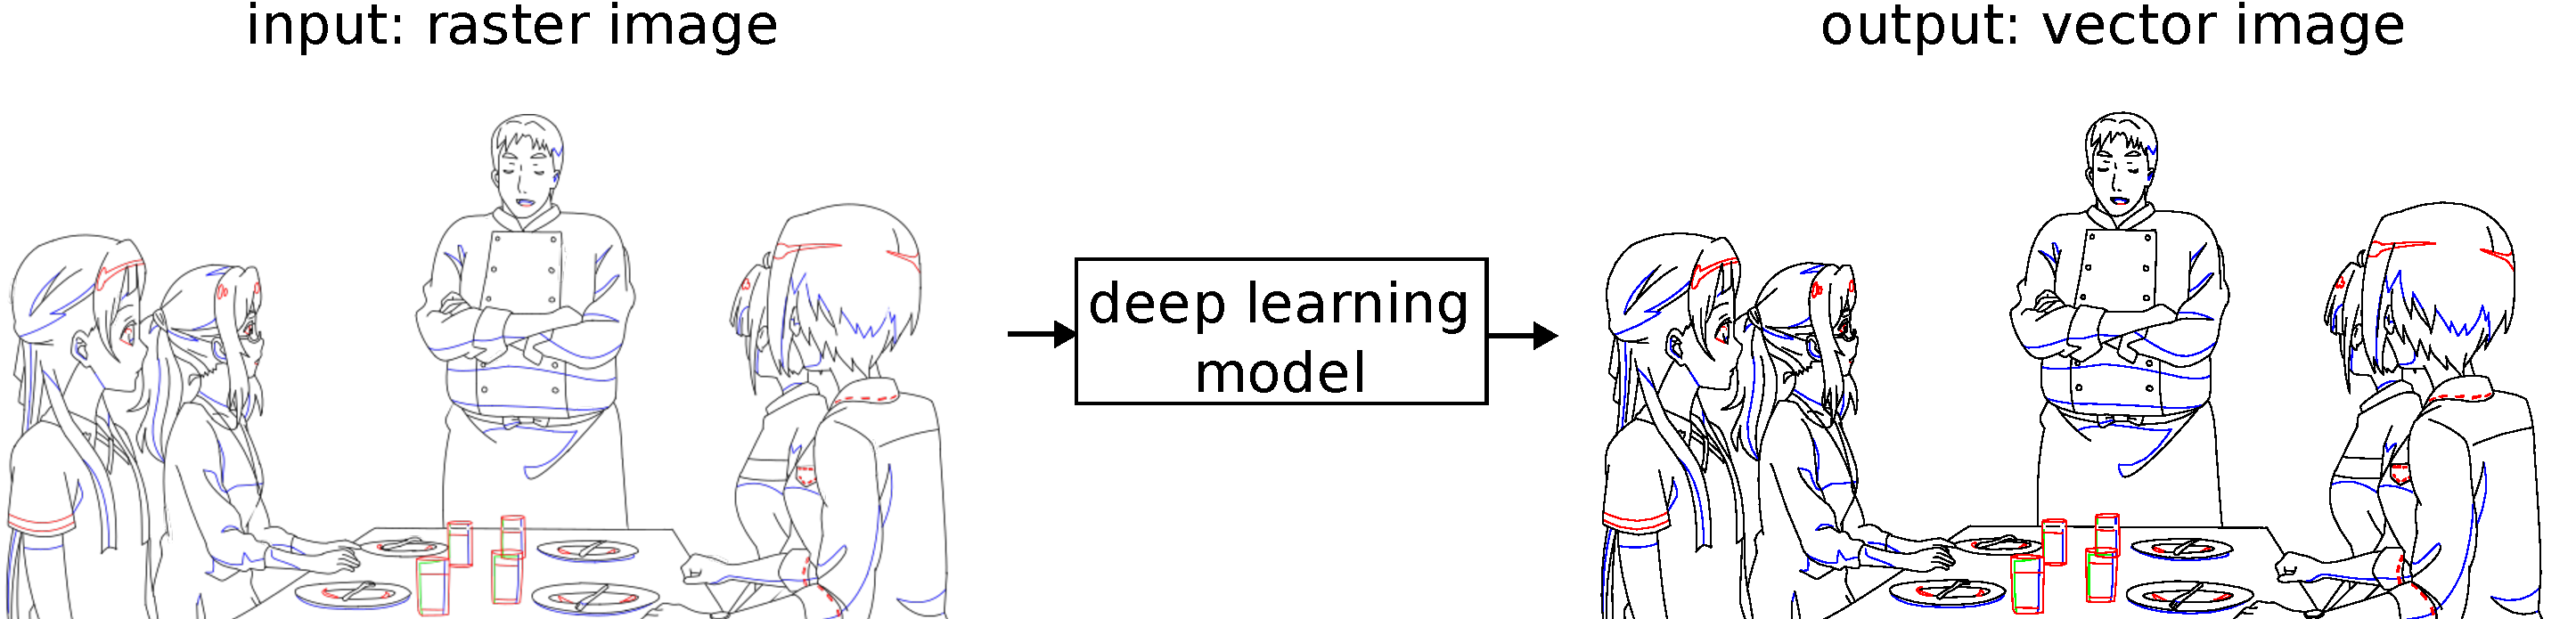
\includegraphics[width=\textwidth]{graphics/work_overview.pdf}
    \caption{The general design of the proposed objective. Input and output images are provided by Tonari Animation.}
    \end{subfigure}
    \begin{subfigure}{\textwidth}
    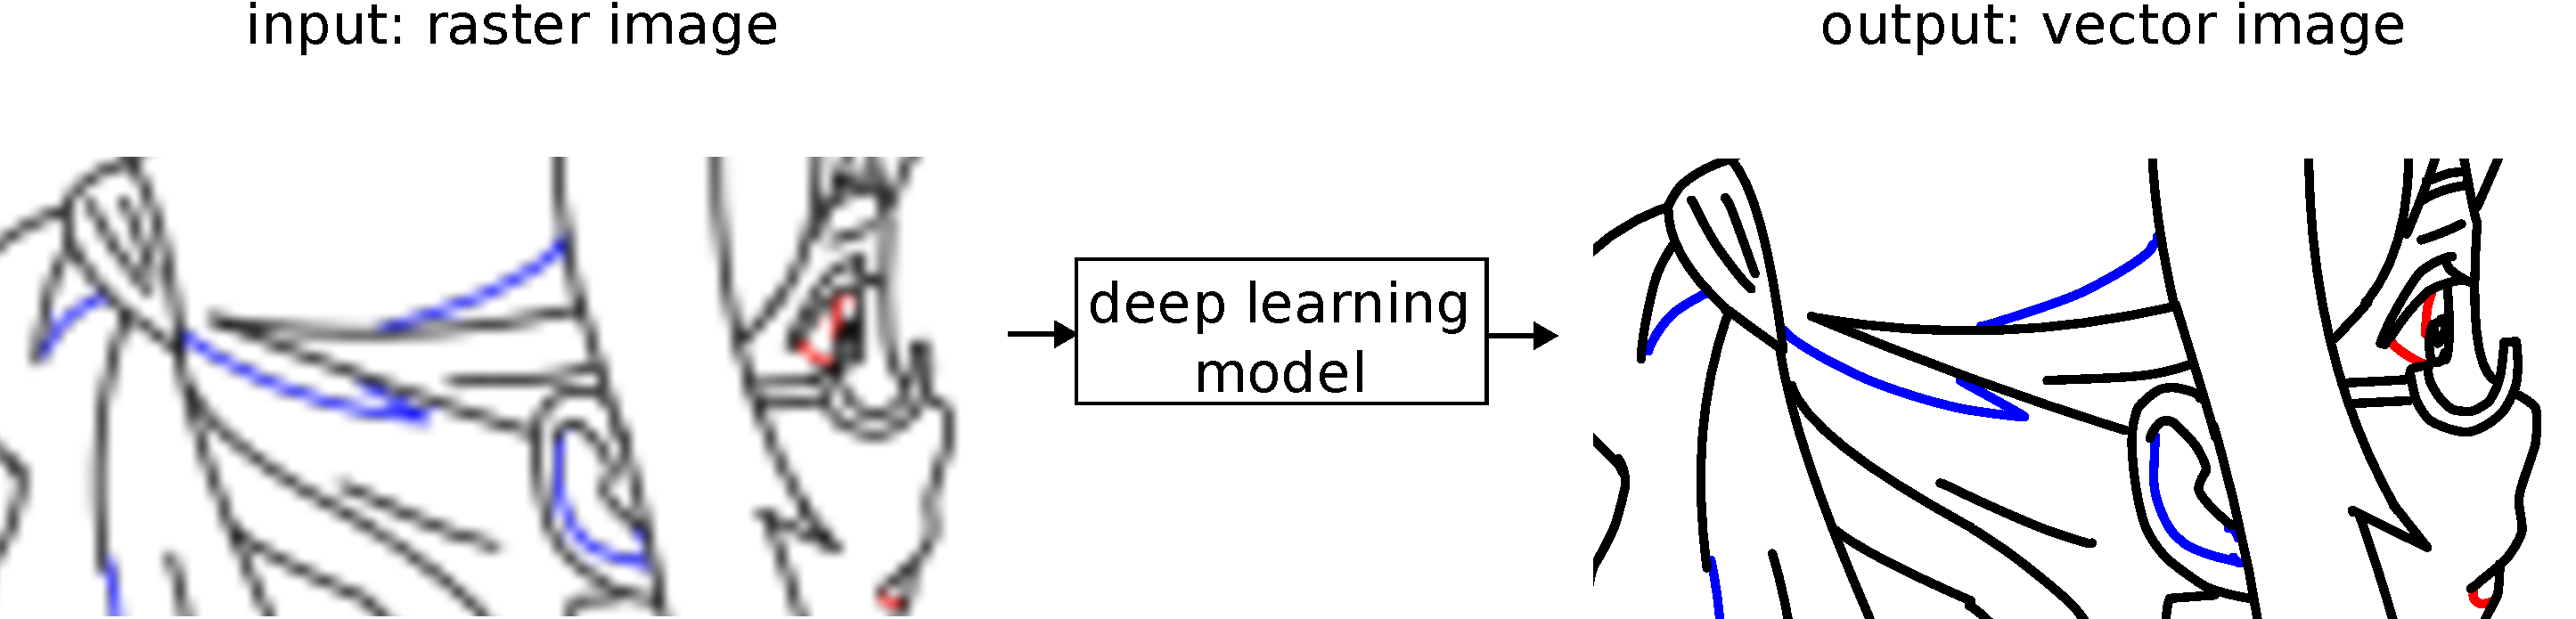
\includegraphics[width=\textwidth]{graphics/work_overview_zoom_8x.pdf}
    \caption{Highlighted section of input and output images, which reveals structural differences.}
    \end{subfigure}
    \caption{Overview of the research objective. The objective is to automatically convert clean animation frame line-art raster images into vector images. Zooming into the figure reveals the structural difference between the input and the output image. Note that the output image is taken from the gold standard test dataset. For a genuine reconstruction result of the developed line-art vectorization method, refer to \Cref{fig:input.output.example}}
    \label{fig:work-overview}
\end{figure}

In principle, animation consists of sequentially showing single frames in order to achieve the visual effect of a moving scene. \emph{Limited animation} is an animation technique in which frames are not completely redrawn (like in full animation), but where the moving parts (also called \emph{cels}) are reused over frames. While both full animation and limited animation techniques reuse some fixed parts (like the background), the reusing of cels by limited animation leads to the characteristic stiff style and reduces the cost to produce an animated series. Today, the technique is primarily used in hand-drawn animations, often under the term \emph{anime} popularized by Japanese media.

While limited animation was mostly replaced with full animation and 3D animation in the western world, it still enjoys continued relevance due to the growing importance of anime. This importance is underlined by \citet{napier2016anime}, who estimates that anime made up over 60 percent of all animated shows in 2016. Unsurprisingly, anime is especially prevalent in Japan, where it accounts for 6 of the top 10 highest-grossing films in 2021 \citep{jpboxoffice}. According to \citet{animeindustryreport}, the worldwide market for anime monotonically grew from 1266.1 billion Yen in 2009 to 2742.5 billion Yen in 2021 (with an exception in the year 2020). This trend suggests that limited animation will continue to be relevant in the future.

The hand-drawn limited-animation production process is composed of four phases. Based on the storyboard produced in the first phase, animators repeatedly draw and improve rough key frames in the second phase. These keyframes are line drawings only drawn for critical moments in a scene and contain mostly cels. In the third phase, the keyframes are vectorized and cleaned. To achieve the visual effect of fluidity, a large number of frames in between the keyframes are drawn. In contrast to full animation, these \emph{inbetweens} are not redrawn completely, but reuse the majority of a keyframe while only editing small parts of the image. Finally, in the fourth phase, the clean frames are colored and enriched with special effects and a background image.

Thus, the production consists of creative parts such as the drawing of keyframes and tedious tasks such as the creation of inbetweens. The latter tasks are a ripe target for automatization, freeing up animation studios to focus on the creative parts of their work. This work explores the automatization of one such task, specifically the vectorization of clean animation frames.

Traditionally, computational tasks are automated using hand-crafted algorithms with manually set parameters. While this is feasible for well-defined and structured tasks, it is unfeasible for complex, ambiguous tasks with high-dimensional data, such as the vectorization of clean animation frames. A different automatization technique that is better fit for these types of tasks is \emph{machine learning}. Contrary to hand-crafted algorithms, machine learning consists of assembling a large dataset of inputs and outputs and defining an algorithm which exploits statistical correlations in this dataset to fit a model that generalizes to data outside of this dataset. A subset of machine learning that has increased in importance in recent years is \emph{deep learning}, in which the model fit to the dataset is an artificial neural network \citep{Rosenblatt58theperceptron}.

In this chapter, \Cref{sec:motivation} provides the motivation for the research. 
\Cref{sec:intro.problem} details the research question and related research objectives. \Cref{sec:challenges} lists the challenges associated with the research objectives. \Cref{sec:intro.goals} gives a summary of the main contributions of this work. Finally, \Cref{sec:intro.structure} outlines the structure of the thesis.

\section{Motivation}
\label{sec:motivation}
%Hand-drawn animation could greatly benefit from machine learning methods, but there are little publicly known success stories. \josh{elaborate the rest of this paragraph bit more} Yet, very little work using machine learning on hand-drawn animation production exists, and existing work focuses on models that operate on final video frames. This comes in clear contrast with research on illustration and comics, for which a lot more research exists.

In order for the limited animation production process to proceed as quickly and as accurately as possible, clean frames need to be drawn as vector images. Contrary to raster images, which represent an image using a raster of color values, vector images represent an image using a hierarchy of graphical primitives. The primitives used in this case are lines and curves. Having the clean frame as vector line art enables accurate and easy editing. Furthermore, vector files are resolution-independent and require less data to represent an image than lossless raster formats, where the color of each pixel needs to be stored somehow. Moreover, by their nature they also contain the semantic composition of the image, which is potentially useful for downstream tasks.

In many animation studios, limited animation frames are initially drawn on paper, i.e., in raster format. Afterwards, these frames need to be manually traced in order to produce clean frames in vector format. This manual conversion is a tedious and time-intensive process, requiring roughly an hour per frame. Hence, it would be beneficial to have a method which can convert the clean frame into vector format automatically.

Even disregarding the step from rough animation frames in raster format to clean frames in vector format, there are scenarios where the clean frame is only available as a raster image. This could be due to various reasons, including discontinuity in the production workflow (e.g., when different studios are contracted for different steps), the need to export an image from the drawing program to another application, or the existence of old production data that needs to be reused.

Once the clean animation frame is available in vector format, it increases the efficiency of successive workflow steps. An example is the creation of the frames inbetween keyframes, where artists can naturally utilize existing keyframes and only edit a small part of the image. As an example, the curves making up strains of hair could simply be moved instead of needing to be completely redrawn in the case of a raster image.

In summary, in the event of clean animation frames being only available in raster format, it is necessary to manually vectorize the images before they can be used efficiently. Therefore, this work explores the possibility of automatizing this laborious process using line-art image vectorization methods. 

\section{Aim of the Work}
\label{sec:intro.problem}

The purpose of this work is to create a method to automatically convert clean animation frame raster images into corresponding vector images. As mentioned in \Cref{fig:work-overview}, this method consists of a deep learning model trained on clean animation frames. For the resulting line-art vector image to be useful for artistic purposes, the content needs to be semantically meaningful, i.e., the arrangement, topology and parameterization of graphical primitives (i.e., lines and curves) need to make sense and be close to how artists would draw. This prevents traditional algorithms \citep{Selinger03potrace:a, autotrace, 10.1145/2421636.2421640} to be used for that purpose, as these often produce vector images that visually resemble the raster image closely, but contain semantically meaningless vector primitives - for example, a naive but visually convincing vectorization solution is to represent each pixel as a small line.

In detail, this work will attempt to answer a \paragraph{\gls{rq1}}, which is to what extent is it possible to automatically vectorize clean animation frame line art in a manner that is semantically meaningful?

\section{Challenges}
\label{sec:challenges}

Creating the deep learning-based method to vectorize clean animation frames represents a challenge in itself, due to the visual structure of the images. Specifically, it is crucial that the output of the proposed deep learning model is structurally similar to real clean frame vector images, i.e., that the output consists solely of the primitives that artists use to draw clean animation frames. Hence, it is necessary to find a representation of these primitives that is suitable for deep learning models.

Another challenge is the low amount of available data. While a small dataset ($N=139$) of raster/vector image pairs of clean frames was provided to us as part of a research project (and drawn at the Tonari Animation studio), this is not a sufficient quantity to fit a deep learning model. Since there is little publicly available data for this task, extending the dataset is non-trivial. In order to achieve this, data augmentation methods have to be used in addition to procuring public data.

Moreover, clean animation frame images often contain a large amount of curves (usually more than 1000 lines per image). The proposed solution needs to be designed in a way to handle this large amount of primitives, since prior deep learning-based works are often suited only for images with a lower amount of curves. 
Additionally, it is necessary for the image vectorization method to be applicable at lower image resolutions, since clean frame raster images (especially older production data) are often at a resolution for which existing algorithms were not designed.
Furthermore, it is unavoidable that the resulting vector images will contain errors and therefore need to be corrected manually. Hence, the solution should focus more on getting the curves it generates correct, rather than covering all curves in the input image. In other words, a solution that generates half of the curves completely correct is preferable to a solution that generates all of the curves only somewhat correct, since in the latter case all curves have to be manually corrected anyway.

Finally, the clean animation frame vectorization method should be designed as a deep learning model, as this makes it easier to adapt it to vectorize raster images from different domains using finetuning. This is important for a related task, which is motivated in the following: One factor that has greatly limited successful attempts in the field of deep learning in hand-drawn limited animation production is the scarce amount of available production data that can be used for training. While it is probably fruitless to attempt to design a system that generates the whole animation automatically, solving individual steps in the production process might be possible. It is clear that training such models would require a large amount of production data, specifically production data that is in reverse order of the actual production workflow. As an example, if a large dataset of clean keyframes and associated inbetweens (as well as animation timesheets) was available, it would be possible to train an inbetween generation model. Other potential uses include clean frame coloring, inpainting or compositing.

While the obvious way of attaining an animation production dataset would be for a studio to publish it, thus far no such dataset has been published, which presents another challenge. An alternative would be to synthesize the data. The differentiable nature of the proposed line-art vectorization algorithm could be utilized for that purpose. While the model will be trained using clean frames as input data, it might be possible to extend or finetune the model to use images of another domain (such as final animation frames) as input. Then, it could be used for a cross-domain vectorization model in order to convert raster images of one domain (e.g., final animation frames) into vector images of another domain (i.e., clean frames). \Cref{fig:cross-domain-overview} depicts such a model. Since final animation frames are readily available in high quantity and quality, this would potentially make it possible to synthesize a large dataset of clean frames requiring only small supervision. However, creating such a model is not the focus of this work, rather, the above-mentioned line-art vectorization method is designed in a way such that it could in principle be extended to cross-domain line-art vectorization. Most importantly, this means that the model is nearly end-to-end differentiable, such that it can be easily finetuned on other data. This is a characteristic that traditional algorithms \citep{Selinger03potrace:a, autotrace, 10.1145/2421636.2421640} do not possess.

In summary, the quantity of the data and the qualitative structure of the data domain impose a range of restrictions which need to be accounted for in the architecture design of the method. Furthermore, the method should be based on a deep learning model in order to enable adaptability to other input data domains.

\begin{figure}
    \centering
    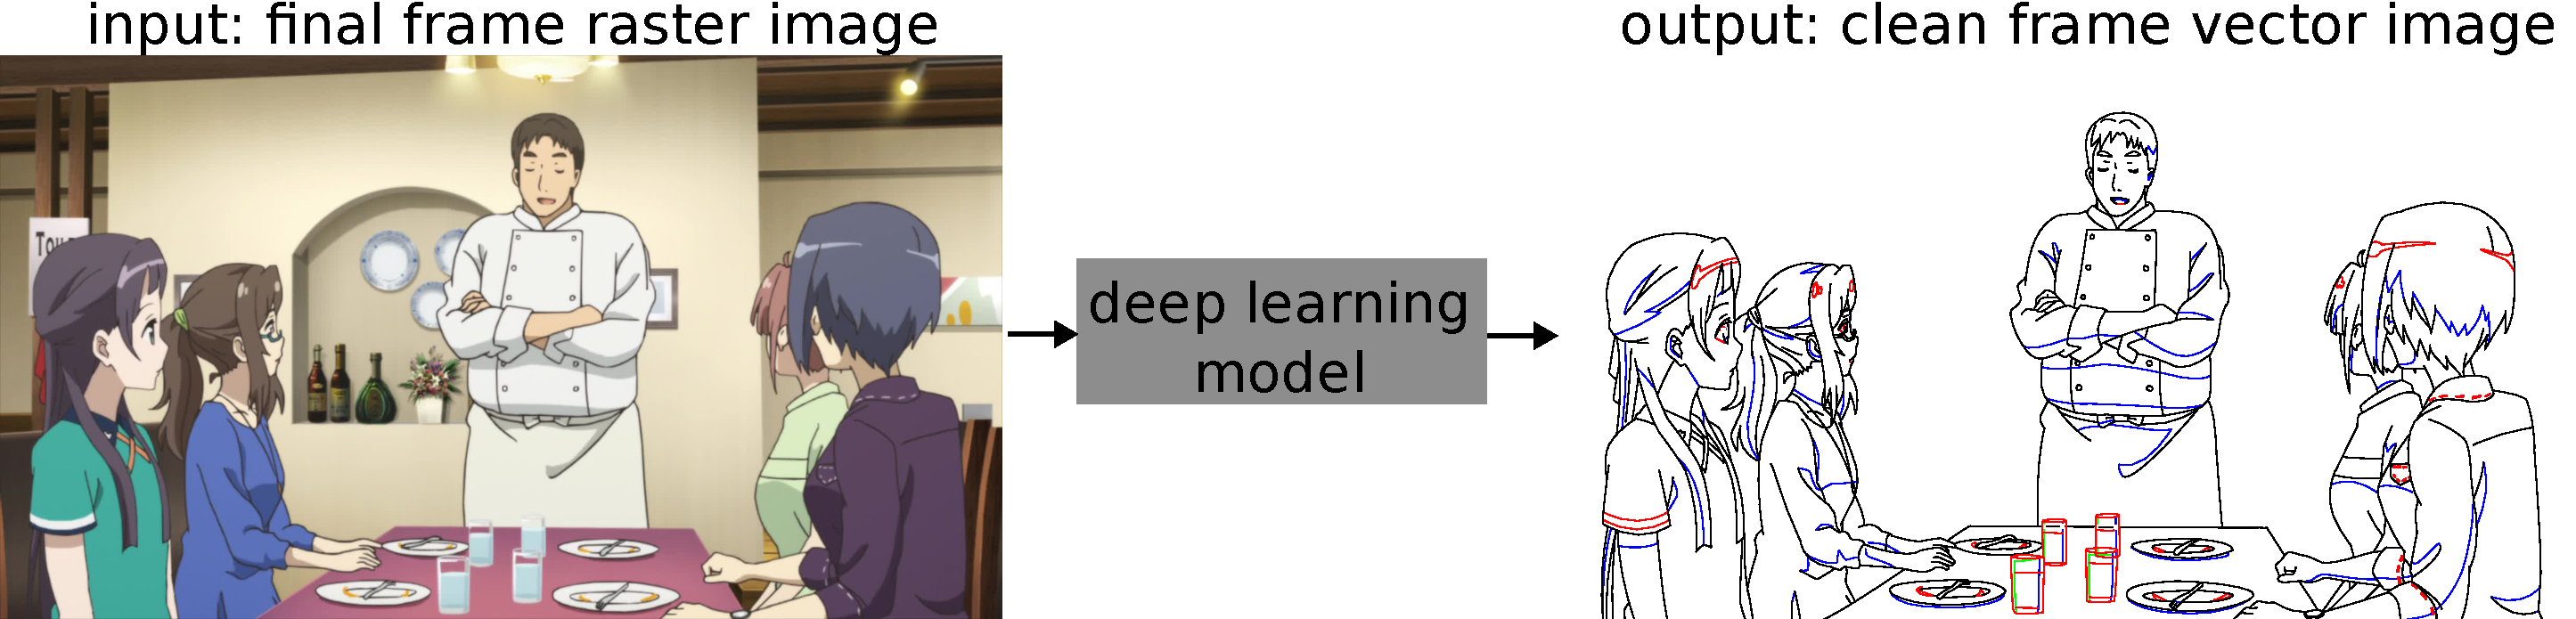
\includegraphics[width=\textwidth]{graphics/cross-domain-overview.pdf}
    \caption{An overview of cross-domain line-art vectorization, a potential extension of the proposed solution. Here, the objective is to convert final animation frame raster images (example by \citet{sakura-quest}) into clean animation frame vector images by extending or finetuning the deep learning model depicted in \Cref{fig:work-overview}.}
    \label{fig:cross-domain-overview}
\end{figure}

\section{Contributions}
\label{sec:intro.goals}

To answer \gls{rq1}, the \gls{ro1} is to create a method for line-art vectorization that takes clean animation frame raster images as input and outputs the corresponding semantically meaningful vector image. This method is described in \Cref{sec:model} and based on a deep learning model to enable it to be adapted to different input image domains. Furthermore, it is designed to fit the qualitative structure of clean animation frames as input and output images. 

Accordingly, the \gls{ro2} is to perform an evaluation that ascertains the extent to which the developed method and existing state-of-the-art line-art image vectorization methods are able to vectorize clean animation frames. This evaluation is described in \Cref{sec:eval}. Great care is taken to ensure that this evaluation is reproducible. Due to this, the whole evaluation is not only conducted on the clean animation frames provided by Tonari Animation, but also on a publicly available subset of the SketchBench \citep{Yan:2020:ABR} dataset. Furthermore, the code for the evaluation is publicly available at \url{https://github.com/nopperl/marked-lineart-vectorization}. Ultimately, while the evaluation shows advantages of the developed line-art image vectorization method compared to existing state-of-the-art methods, no method is able to satisfactorily vectorize clean animation frames.

\paragraph{\gls{ro1}} A deep learning-based method for clean animation line-art vectorization.
\paragraph{\gls{ro2}} A reproducible evaluation assessing the extent to which line-art image vectorization methods can vectorize clean animation frames.

\section{Structure}
\label{sec:intro.structure}

\Cref{ch:bg} describes the necessary prerequisites required to understand the proposed solution. \Cref{ch:related} gives an overview of prior work related to the research objectives. The proposed solution is described and empirically evaluated together with state-of-the-art methods in \Cref{ch:alg}. \Cref{ch:conclusio} revisits the research objectives, lists limitations and provides potential future work.

\chapter{Background}
\label{ch:bg}
This chapter details the theoretical background of clean animation frame vectorization.  \Cref{sec:bg.vec} gives an overview of both raster and vector images as well as the process of vectorization, i.e., converting raster images to vector images. \Cref{sec:anime.prod} describes the process for hand-drawn limited animation in more detail. \Cref{sec:bg.dl} explains deep learning, which is the technique used in this work to develop an automatic clean animation frame vectorization method.

\section{Vectorization}
\label{sec:bg.vec}

In a digital context, images can be  represented using either \emph{raster} or \emph{vector} data formats. These are introduced in \Cref{sec:bg.vec.raster,subsec:bg.vector}, respectively. This work is concerned with \emph{image vectorization}, i.e., the conversion of raster images into corresponding vector images, which is described in \Cref{sec:vec}.

\subsection{Raster Images}
\label{sec:bg.vec.raster}

\begin{figure}
    \centering
    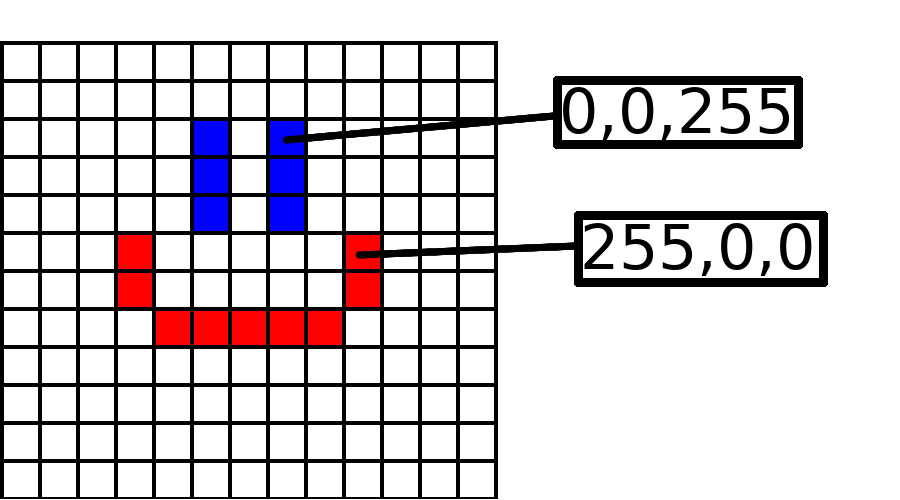
\includegraphics{graphics/raster_color_ex.png}
    \caption{Example of an image represented using a raster of 13x12 pixels. Notice that color information is stored explicitly per pixel.}
    \label{fig:raster-color-ex}
\end{figure}

Digital visual data are most commonly represented using \emph{raster} data formats. Raster images store visual data as a \emph{raster}, a 2-dimensional grid of uniformly sized squares. Each of these squares can be referred to as \emph{pixel} and is defined by its location and its color.

\begin{figure}
    \centering
    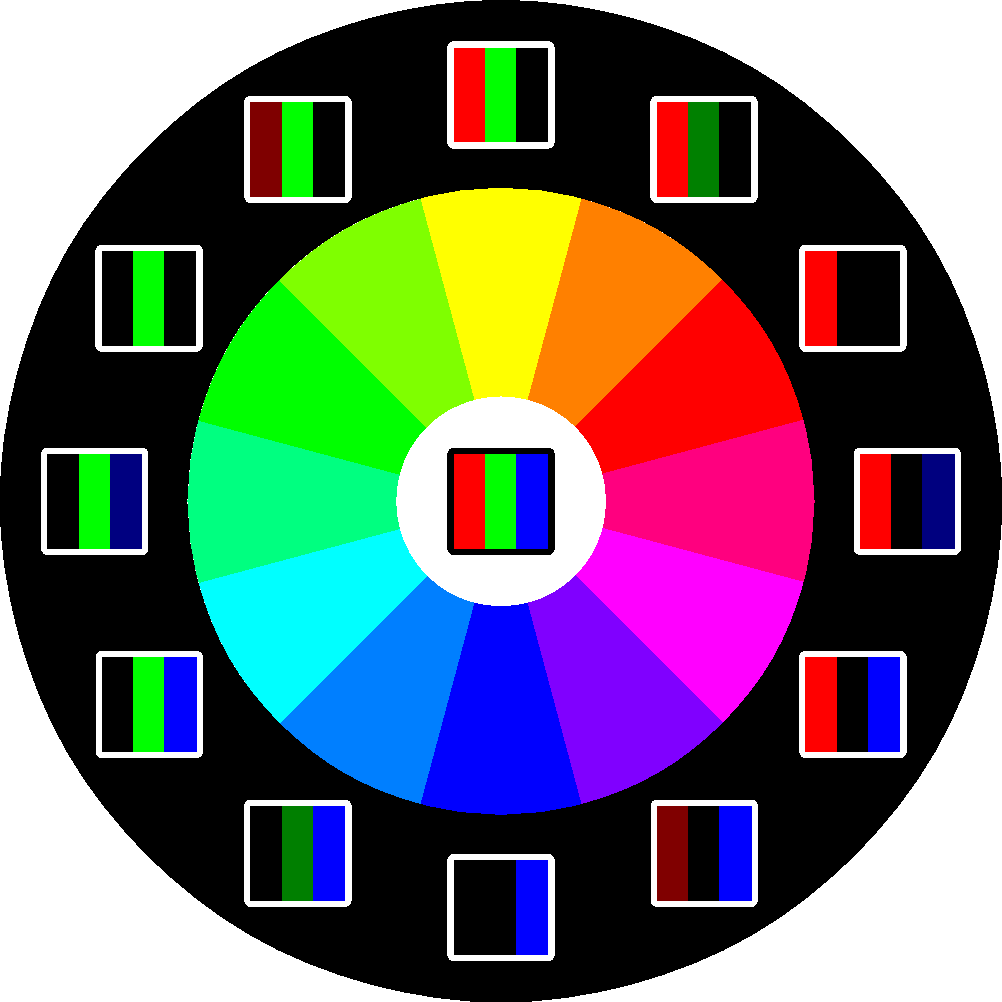
\includegraphics[width=0.5\textwidth]{graphics/RGB_color_wheel_pixel_30.pdf}
    \caption{A color wheel exemplifying the \gls{rgb} color model. The box next to each color displays the intensities of the red, green and blue component respectively (with black indicating zero intensity). The three components are added in order to produce the displayed color. Created by \citet{nemethcolorwheel}.}
    \label{fig:rgb}
\end{figure}

Raster images can be naively stored using numerical two-dimensional arrays or matrices. The pixels location in the array is directly mapped to the location on the grid (and therefore on the display). This way, the only information that needs to be stored explicitly for each pixel is its color. Usually, a color is defined using a \emph{color model} such as the \gls{rgb} or the CMYK model. In the case of \gls{rgb}, a color is defined as the intensity of each of the components red, green and blue. These components are then mixed according to their respective intensity using simple addition to produce a color. Using this additive model, a broad spectrum of colors can be represented using only 3 numerical values. This is shown in \Cref{fig:rgb}. Furthermore, the numerical values are bounded and usually in $[0,1]$ (representing relative amounts) or in $[0,255]$ (in absolute amounts, intentionally the maximum amount which can be stored in a bit). This data format is exemplified in \Cref{fig:raster-color-ex}.

There exist multiple ways of storing raster images. The naive storage format mentioned above is referred to as bitmap. Since the location of each pixel of the grid is implicitly given, the only information that needs to be stored is the color (i.e., three numerical values) per pixel. Other formats such as the commonly used \gls{png} \citep{RFC2083} or JPEG attempt to reduce the necessary storage space using compression algorithms. The format can also be extended to include opacity (i.e., transparency) as an additional fourth component of the color model (then referred to as RGBA color model). The grid (and in turn the array) can also be extended by a third dimension in order to represent three-dimensional graphics (referred to as \emph{voxel data}).

\subsection{Vector Images}
\label{subsec:bg.vector}

\begin{figure}[h]
\centering
\begin{subfigure}[b]{0.4\textwidth}
\centering

\includegraphics[]{graphics/vector_ex.pdf}
    \caption{A vector image consisting of 5 shapes.}
    \label{fig:vector-ex.vec}
\end{subfigure}
\hfill
\begin{subfigure}[b]{0.4\textwidth}
\centering
    
\includegraphics{graphics/vector_ex.png}
    \caption{A raster image consisting of 50x50 pixels}
\end{subfigure}
    \caption{An example image in both vector and raster format. By zooming in, it is possible to experience the fundamental difference between the two formats.}
    \label{fig:vector-ex}
\end{figure}

A different way to represent images are vector images. In contrast to raster formats, vector data formats represent images using graphical primitives. These primitives are the most basic geometries which constitute images, such as points, lines or polygons. Using these low-level primitives, it is also possible to define higher-level shapes like text, circles or parametric curves. Each primitive or shape can carry attributes such as the color it is filled with, location or size. These primitives can be arranged both in a hierarchical and in a topological structure, i.e., their spatial relations can be explicitly defined. \Cref{fig:vector-ex} gives an example of an image in both vector and raster format. The vector image in \Cref{fig:vector-ex.vec} is stored using a vector format called \gls{svg} \citep{w3csvg}, which is developed by the World Wide Web Consortium and is widely used, especially on the world wide web. The underlying \gls{svg} contents can are shown in \Cref{lst:vector-ex-svg}. Note that, in contrast to storing each pixel and its color, the \gls{svg} file stores way less data. 

\begin{listing}
\begin{minted}{xml}
<?xml version="1.0" encoding="UTF-8" standalone="no"?>

<svg
   width="100"
   height="100"
   version="1.1"
   xmlns="http://www.w3.org/2000/svg"
   xmlns:svg="http://www.w3.org/2000/svg">
<circle
   style="fill:#ffee00;stroke-width:0.264999;fill-opacity:1"
   cx="13.658114"
   cy="13.587115"
   r="10" />
<path
   style="stroke:#000000;stroke-width:0.27px;stroke-linejoin:miter"
   d="m 5.42,14.74 c 3.75,8.27 12.45,8.06 17.34,0.038" />
<ellipse
   style="fill:#0000ff;fill-opacity:1;stroke-width:0.324317"
   cx="11.310536"
   cy="11.553639"
   rx="1.3157237"
   ry="2.5536389" />
<ellipse
   style="fill:#0000ff;fill-opacity:1;stroke-width:0.324317"
   cx="15.776539"
   cy="11.553638"
   rx="1.3157237"
   ry="2.5536389" />
<path
   style="fill:#ff00ff;fill-opacity:1;stroke-width:0.264999"
   d="m 11.728484,16.514472 1.290489,2.182378 -2.535239,0.02641 z" />
</svg>
\end{minted}
\caption{The image displayed in \Cref{fig:vector-ex.vec} as \gls{svg} file.}
\label{lst:vector-ex-svg}
\end{listing}


Vector images possess specific advantages over raster images, depending on the context they are used in. The advantages arise from the fact that the image is represented using only a few graphical primitives and their mutual relations.

\paragraph{Small storage size} A vector image is generally smaller than a raster image, since in contrast to raster images it does not describe each pixel, rather only the primitives and their relations. In general, it holds that if the number of primitives required to represent an image is roughly at least less than the number of pixels, the storage size of the vector image will be lower than the corresponding raster image.

\paragraph{Easy editability} The primitives and structure of a vector image can be easily loaded and edited, which is not the case for raster images, which can only be edited at a pixel level.

\paragraph{Resolution-independence} Since the vector image only defines graphical primitives without an explicit raster, it is independent of the resolution of the raster it is displayed on. That means that vector images can be zoomed in indefinitely without losing their apparent quality, or smoothness. In contrast, zooming into a raster image will quickly reveal non-smooth parts.

It is important to note that the above-mentioned advantages are not intrinsic to the vector format itself. The nature of vector formats (and in turn, their advantages) can be reduced ad absurdum. For example, consider a vector format which stores images using the graphical primitive of squares only. A size, fill color and location can be defined for each of these squares. If these squares are then arranged in a grid and of uniform size, this vector image is in essence a raster image in vector format. Viewed another way, a raster image could be considered an optimized way to store such a naive vector image, since in raster formats the size and location of each square does not need to be explicitly stored. To conclude this thought experiment, it is important to note that such a naive vector format loses most advantages associated with vector images (i.e., resolution-independence, easy editability and smaller storage size). Hence, the advantages of vector formats are not intrinsic to their representation of images, rather, each specific vector image needs to be defined using primitives that match the semantic composition of the image, not just the visual appearance.

To reiterate the above conclusion, an important characteristic of a good-quality vector image is that it consists of semantically meaningful primitives and structure. That is, a vector image should describe the visual components using appropriate primitives intuitive to humans (in addition to their mutual relations) and not just match the visual appearance perfectly on a pixel-level. Not only does this provide a high-level description of visual content, but it also reduces the storage space required and retains the important resolution-independence. However, it is clear that these advantages are only given if the visual can actually be represented using the graphical primitives given by the vector format. Hence, there is no general superiority of one image format over the other. Rather, whether vector or raster formats are appropriate always depends on the given task.

\begin{figure}
    \centering
    
\includegraphics[width=0.5\textwidth]{graphics/Art_freeform_baseline_09_Santiago Rial_norm_cleaned.pdf}
    \caption{Example of line art. Drawn by Santiago Rial \citep{Yan:2020:ABR}.}
    \label{fig:line-art-ex}
\end{figure}

An example of an image domain which is appropriate to be displayed using vector formats is line art. This category subsumes drawings that depict objects using lines and curves contrasted with more plain backgrounds. An example is shown in \Cref{fig:line-art-ex}. This visual style is used for a variety of purposes, such as comics, novel illustrations, technical drawings and also animation frames of cartoons. Since line art intentionally attempts to depict objects using simple primitives, it is uniquely suited to be represented using vector formats.


\subsection{Vectorizaton}
\label{sec:vec}

\begin{figure}[h]
    \centering
    \begin{tikzpicture}
    \coordinate (raster) at (0,0);
    \node[label={raster image}] (raster) {
\includegraphics[width=0.2\textwidth]{graphics/vector_ex.png}};
    \node[right=of raster, label={vector image}] (vector) at (5,0) {
\includegraphics[width=0.2\textwidth]{graphics/vector_ex.pdf}};
    \draw [->, lightgray, line width=10pt] (raster) to node[black]{vectorization} (vector);
    \draw [->, lightgray, line width=10pt] (6,-1) to node[black]{rasterization} (1.5,-1);
    \end{tikzpicture}
    \caption{The process of vectorization and rasterization.}
    \label{fig:vectorization-process}
\end{figure}

Image vectorization - also referred to as \emph{image tracing} - is the process of converting a raster image to a vector image. The inverse of this process (converting a vector into a raster image) is referred to as \emph{rasterization}. The process is depicted visually in \Cref{fig:vectorization-process}. There exists a non-injective relation between vector images and raster images, i.e., for each vector image, there exists a corresponding raster image, but multiple vector images can have the same corresponding raster image. In turn, for each raster image, there can be multiple corresponding vector images. Therefore, it is always possible to convert a given vector image into the corresponding raster image. However, when converting a raster image into a vector image, there exists multiple (in essence, infinite) potential corresponding candidates.

Since there is a non-unique set of vector images that map to the same raster image, it is non-trivial to ascertain the quality of the vectorization result. As explained in \Cref{subsec:bg.vector}, in order for the resulting vector image to actually benefit from the advantages of the format, the primitives and structure need to be semantically meaningful with respect to a specific usage. Traditional vectorization algorithms attempt to approximate meaningful primitives using surrogate heuristics, whereas learned algorithms attempt to exploit statistical correspondences in the training data to derive a meaningful result. In general, measuring the primitives and structure of a generated vector image is highly dependent on the intended usage of the vector image.

It is important to note that most displays used today are raster displays. Hence, in order to actually view a vector image on a display, it is necessary to rasterize the vector image. However, most viewing software does not rasterize the vector image a priori, instead, it is interpreted and lazily rendered at the zoom and position level indicated by the user. This can be experienced by zooming into a vector image in this document.

\section{Limited Animation Production}
\label{sec:anime.prod}

\begin{figure}[h]
    \centering
    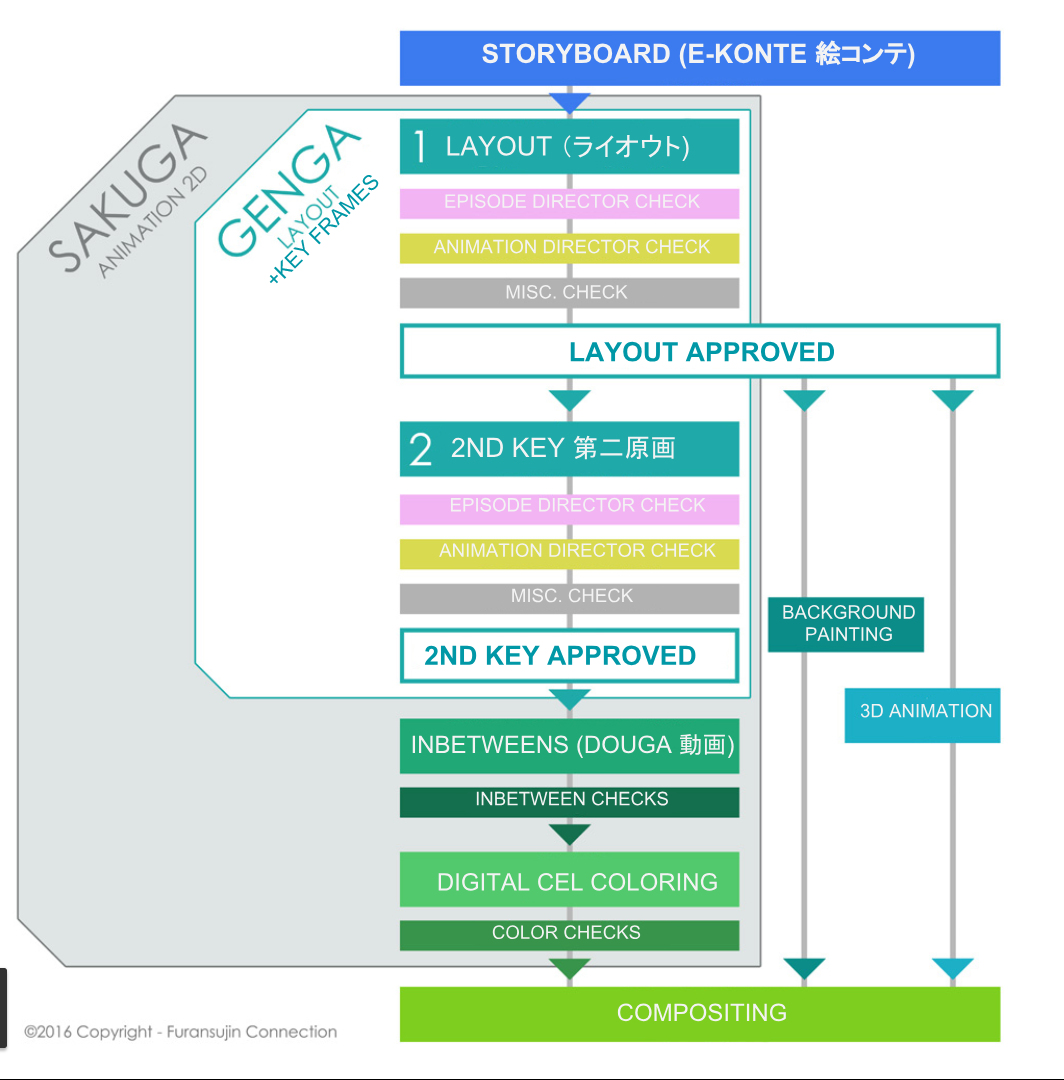
\includegraphics[width=\columnwidth]{graphics/workflow.png}
    \caption{Example of a limited animation production workflow \citep{etapes_fabrication}. The steps dealing with Sakuga (i.e., the steps following \emph{2ND KEY APPROVED} and before \emph{COMPOSITING}) are usually done using vector images.}
    \label{fig:workflow}
\end{figure}

Limited animation is an animation technique in which moving parts (or, \emph{cels}) of a drawing are reused across multiple frames. This stands in contrast to full animation, in which every frame is completely redrawn, which leads to a more fluid animation style. Hence, in order to provide a compelling experience for viewers, limited animation has to rely more on visual \emph{tricks} such as rich backgrounds (which mostly remain still within a scene and therefore can be reused).

\Cref{fig:workflow} gives an overview of the typical production process for hand-drawn limited animation. Note that since limited animation enjoys wide application in the Japanese animation industry, it contains both English and corresponding Japanese production terms. The process starts with the director creating a storyboard, which contains very rough sketches giving an overview of the animation sequence. Based on the storyboard, the key animator draws the layout (or, \emph{1st key animation}) on paper. It encompasses all keyframes in a given scene (also referred to as \emph{cut}), as well as instructions for later stages (such as camera movement). The keyframes themselves do not produce fluid animation, since they are only drawn for critical stages within an animation sequence (beginning, junctures and end). The 1st key frames already include rough sketches for the background as well as the cels. The layout is then normally checked and possibly corrected by the animation director. After the layout is approved, the rough 1st key frames are cleaned up while taking the animation director's corrections into account in order to produce 2nd key animation frames. This process can be repeated multiple times, until the animation director finally approves the keyframes.

% \begin{figure}[h]
%     \centering
%     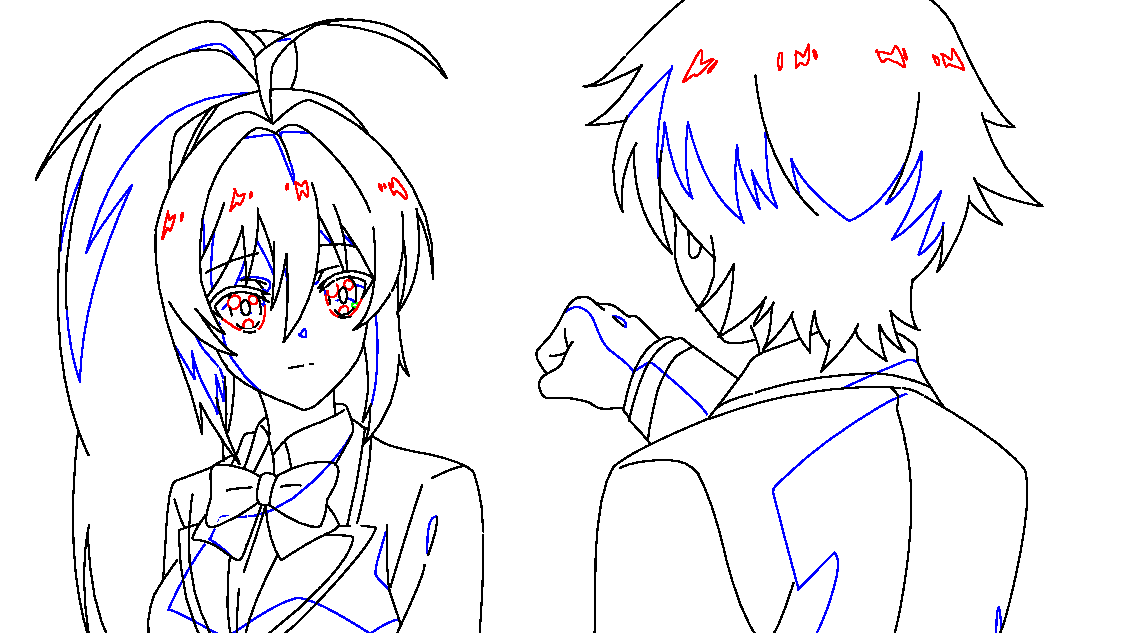
\includegraphics[width=\textwidth]{graphics/douga/39.pdf}
% %    \def\svgwidth{\columnwidth}
% %    \input{graphics/douga/49.pdf_tex}
% %    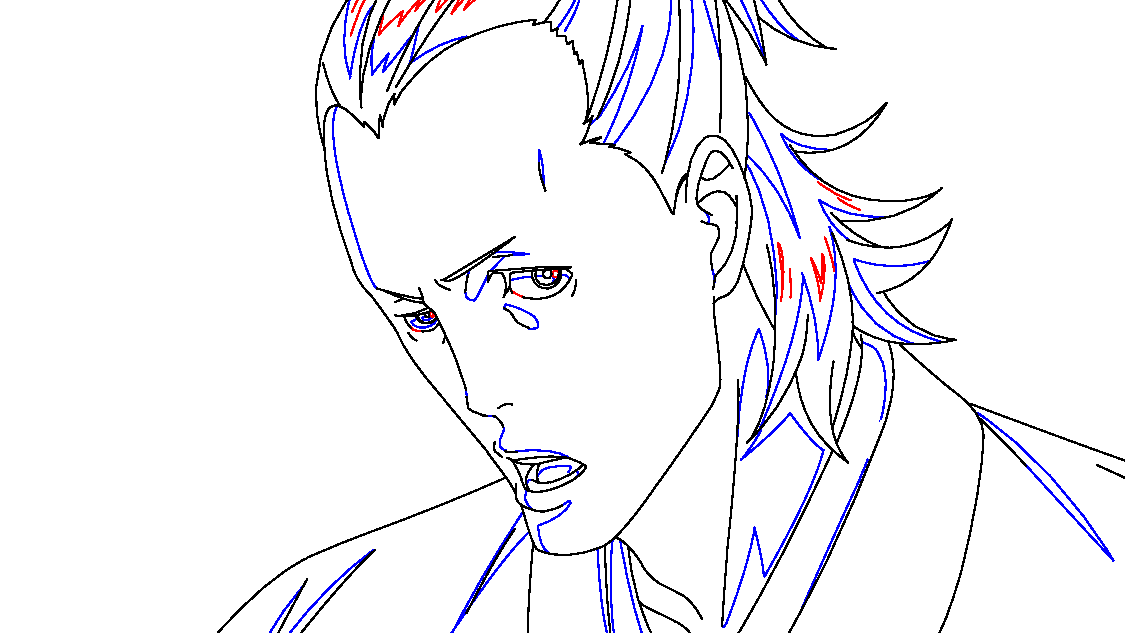
\includegraphics[]{graphics/douga/49.pdf}
% %    \includesvg[inkscapelatex=false]{graphics/douga/49.svg}
%     \caption{A clean animation keyframe in vector format. (© Tonari Animation)}
%     \label{fig:douga.example}
% \end{figure}

% \begin{figure}
%     \begin{subfigure}[b]{\textwidth}
%     \def\svgwidth{\textwidth}
%             \input{graphics/douga/48.pdf_tex}
%     \caption{Caption}
%     \end{subfigure}
%     \vfill
%     \begin{subfigure}[b]{\textwidth}
%     \def\svgwidth{\textwidth}
%             \input{graphics/douga/49.pdf_tex}
%     \caption{Caption}
%     \end{subfigure}
% \label{fig:dougaex}
% \caption{Two examples}
% \end{figure}

\begin{figure}[h!]
    \begin{subfigure}[b]{\textwidth}
    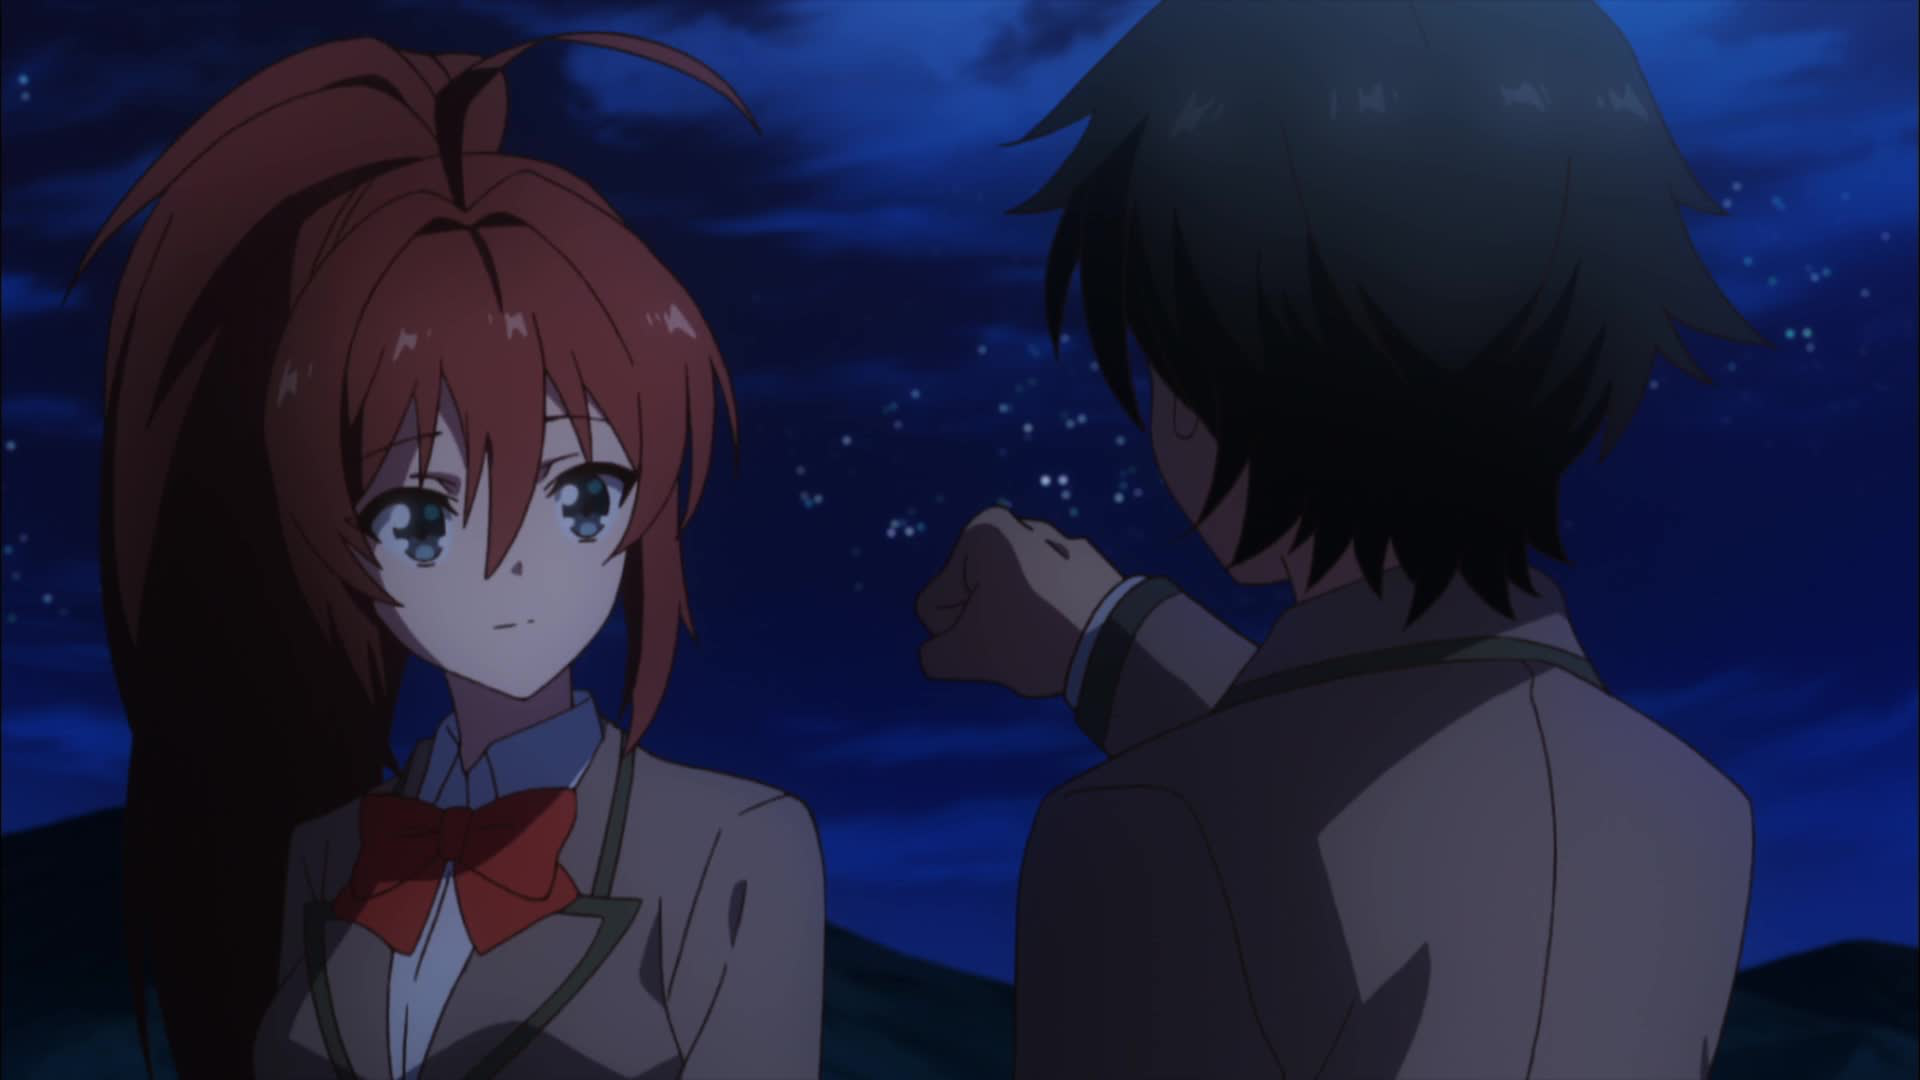
\includegraphics[width=\textwidth]{graphics/douga/39.png}
    \caption{A final composed animation frame by \citet{isekai-cheat-magician}, which is in raster format by default.}
    \label{fig:douga.example.final}
    \end{subfigure}
    \vfill
    \begin{subfigure}[b]{\textwidth}
    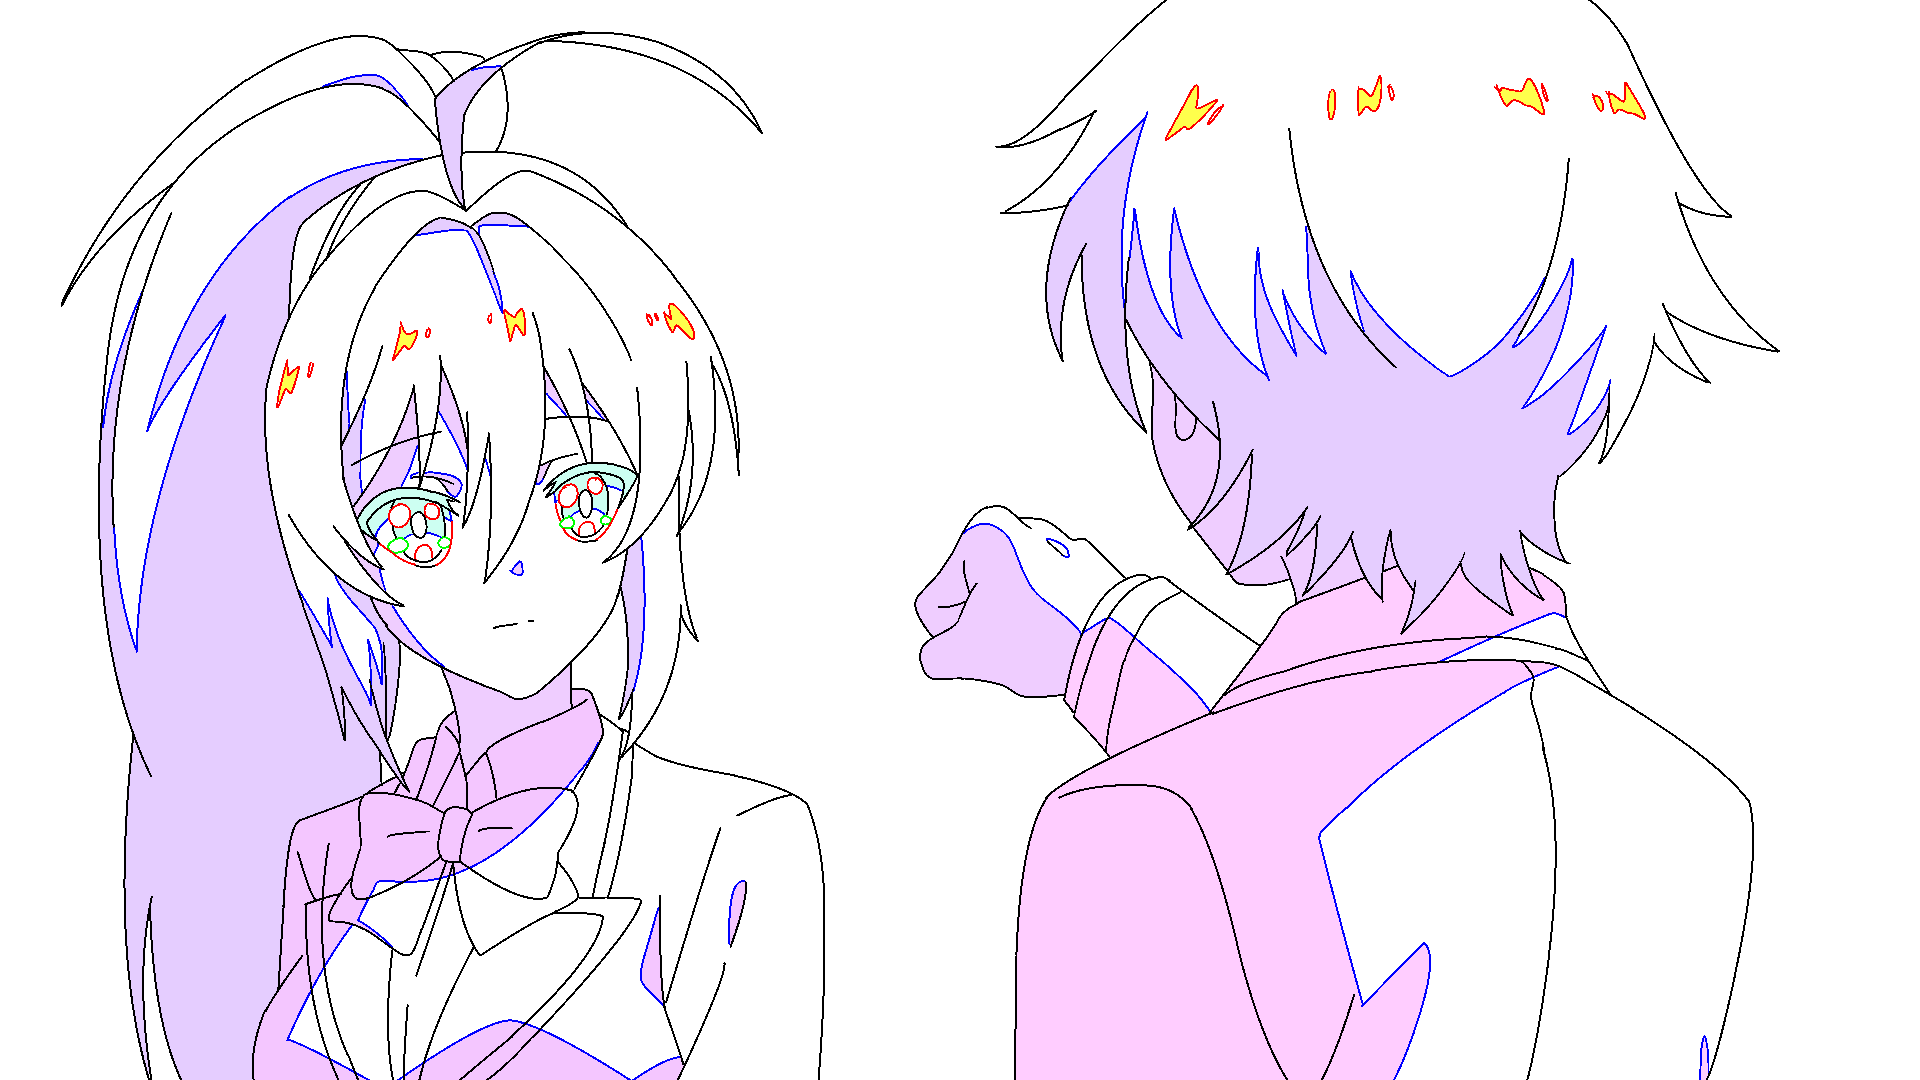
\includegraphics[width=\textwidth]{graphics/douga/836.19.png}
    \caption{The corresponding re-imagined clean animation keyframe in raster format provided by Tonari Animation.}
    \label{fig:douga.example.clean}
    \end{subfigure}
\caption{An example of a clean animation keyframe and the corresponding final animation frame.}
\label{fig:douga.example}
\end{figure}


Afterwards, the approved keyframes are retraced and digitized as vector images. These clean final frames are not full drawings, but include the outlines of each object in a scene, decorative lines, as well as lines indicating shadows, lighting and color regions. It can be interpreted as a semantic description of the essential parts (mostly cels) of the final frame. An example can be seen in \Cref{fig:douga.example.clean}. 

The keyframes are retraced as vector images since this format makes it easy to apply succeeding steps in the workflow. Vector images can be easily and accurately edited by simply altering primitives. Furthermore, images are often worked on at different scales, where the resolution-independent nature of vector images is beneficial. This is especially important when working on tiny details of the image.

\begin{figure}[h]
    \begin{subfigure}[b]{0.3\textwidth}
    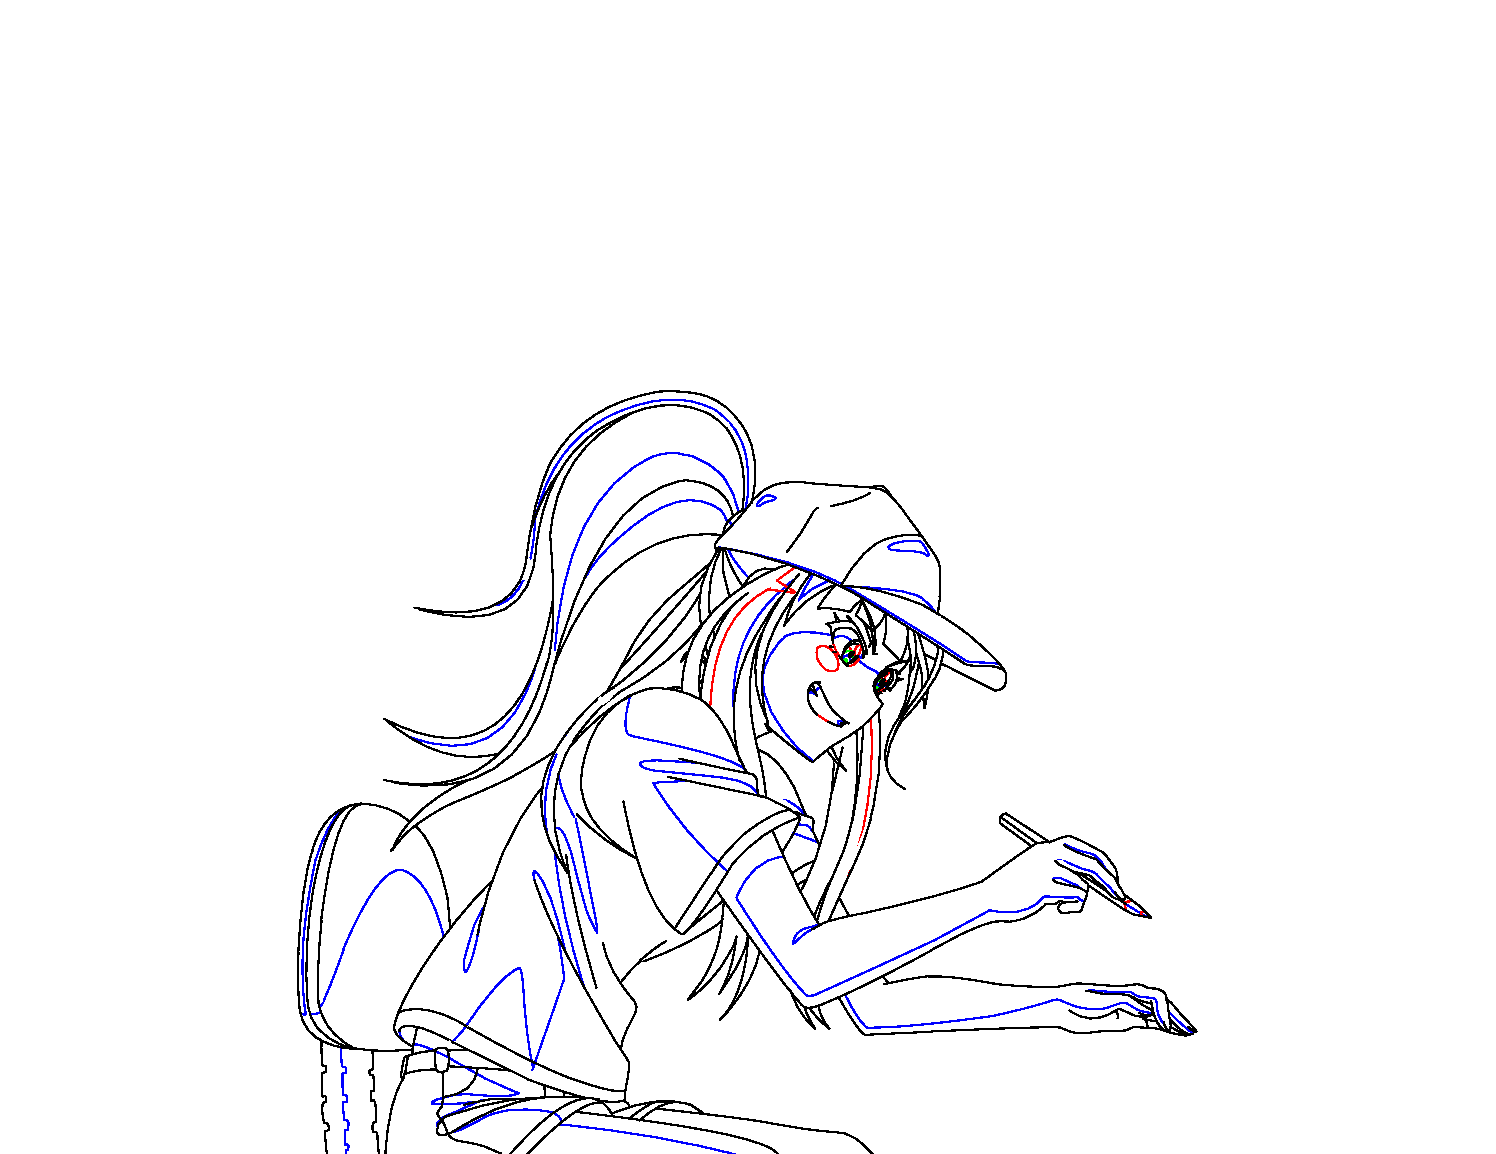
\includegraphics[width=\textwidth]{graphics/douga/007AD_DOU_26.pdf}
    \end{subfigure}
    \begin{subfigure}[b]{0.3\textwidth}
    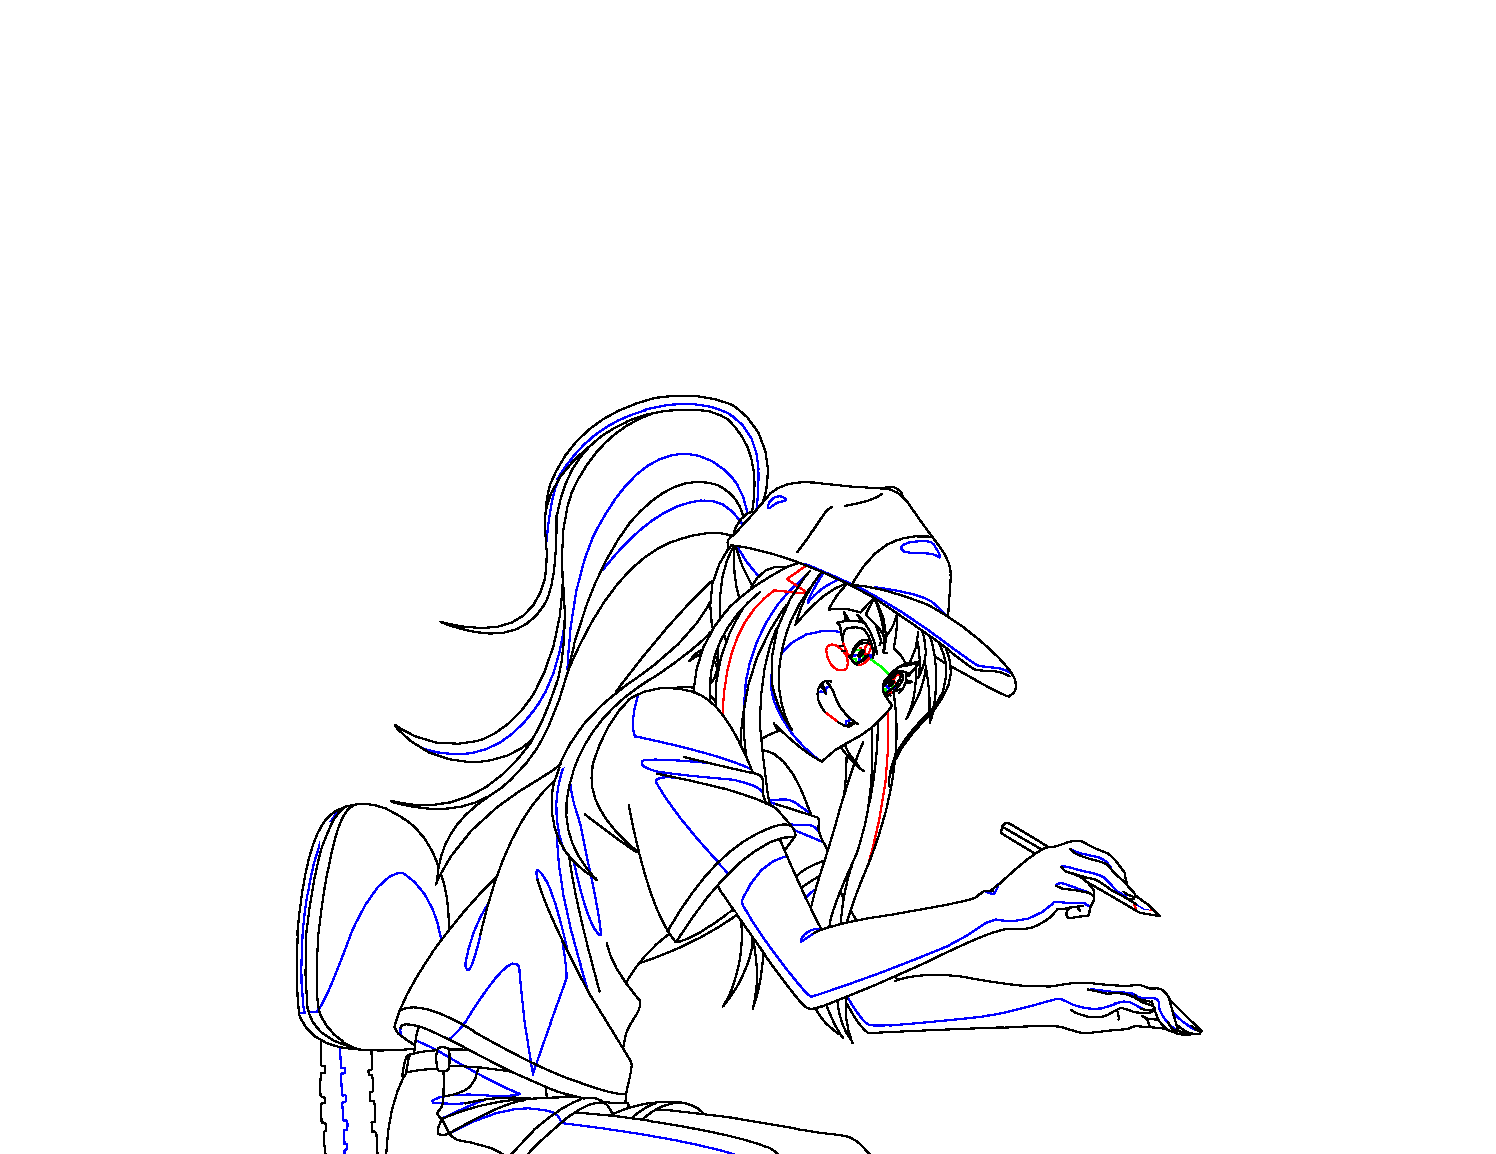
\includegraphics[width=\textwidth]{graphics/douga/007AD_DOU_27.pdf}
    \end{subfigure}
    \begin{subfigure}[b]{0.3\textwidth}
    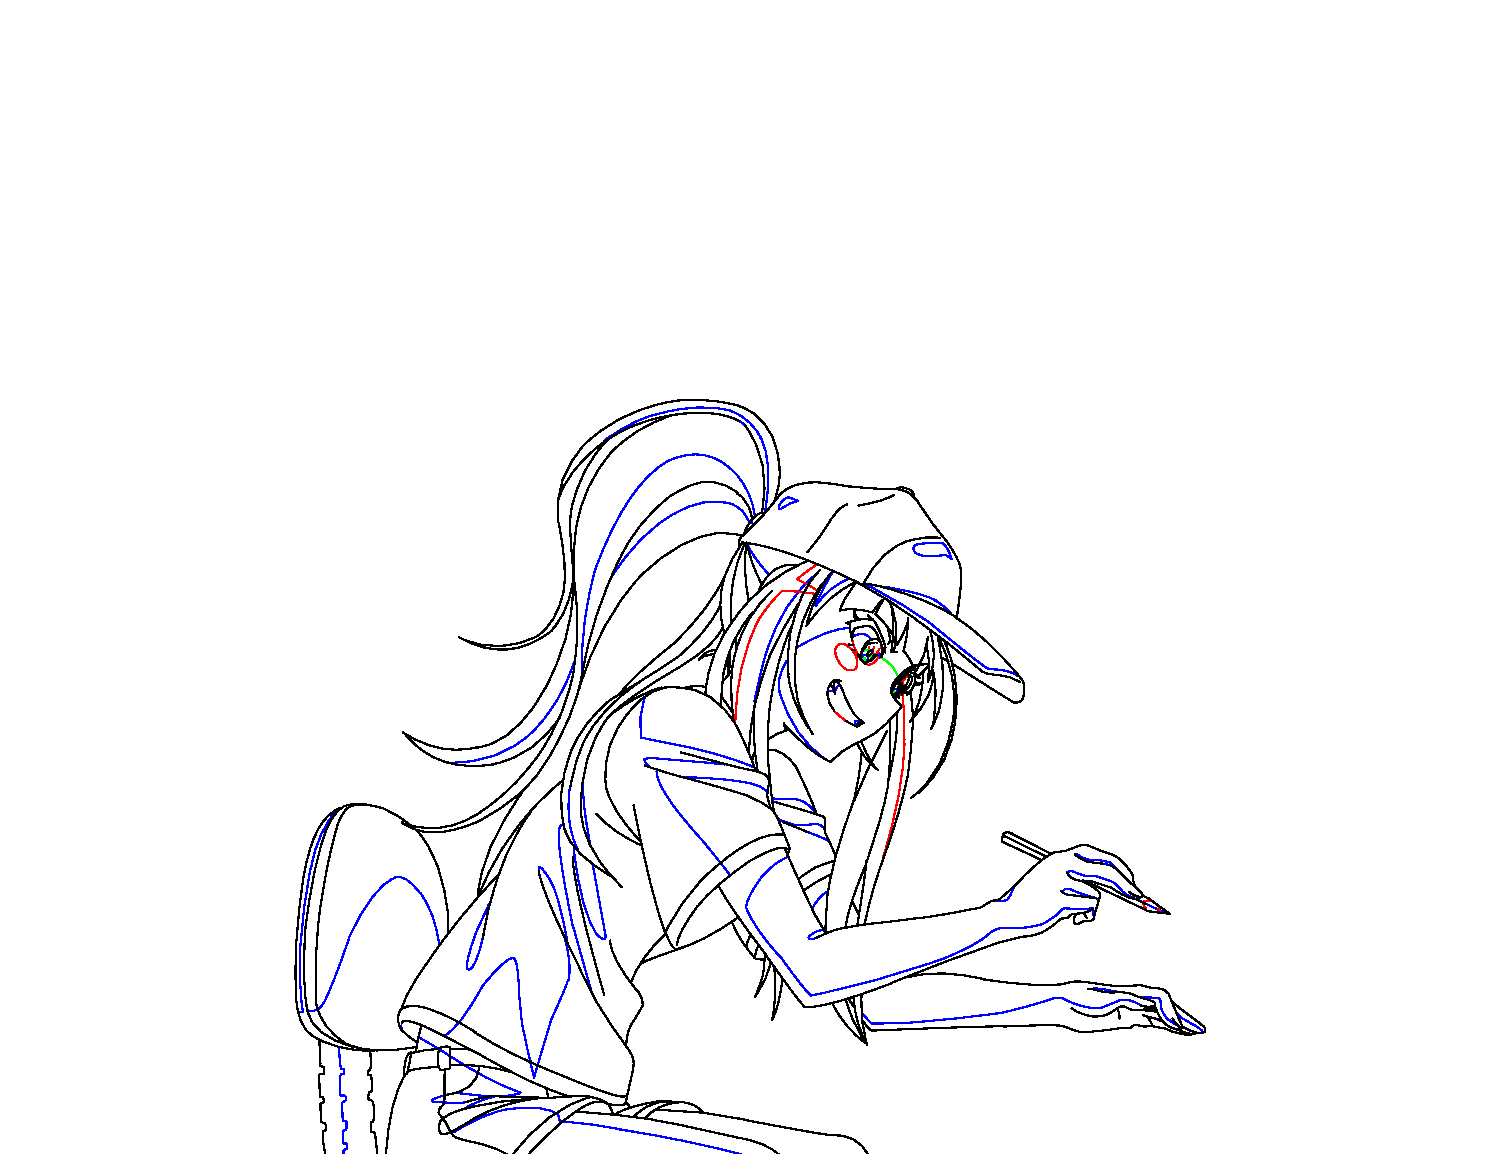
\includegraphics[width=\textwidth]{graphics/douga/007AD_DOU_28.pdf}
    \end{subfigure}
\caption{Three successive clean frames of an animation scene in vector format provided by Tonari Animation. If rapidly shown in succession, the person appears to be moving. Notice minor differences among them, such as the angle of the pencil or the location of strains of hair.}
\label{fig:multiple-douga}
\end{figure}

While up to now only keyframes were drawn, in order to produce fluid movement between them, \emph{inbetweens} are created using the clean keyframes as reference. This is done at such a late stage in order to speed up the process (since only keyframes need to be revised and refined in the initial steps as opposed to all frames). Inbetweens need to be drawn exactly like the keyframe, while having small deviations for moving parts. For the workflow succeeding this step, there is no distinction between keyframes and inbetweens anymore. The resulting images are referred to by various terms interchangeably; most consistently used is the term \emph{douga} (\begin{CJK}{UTF8}{min}動画\end{CJK}, lit. \emph{moving image}) in Japanese limited animation production. \Cref{fig:multiple-douga} depicts three examples of \emph{douga}.

After the clean frames are drawn and approved, they are colored according to their color indications. The color indications in the key animations serve to retain temporal consistency for the coloring. Nowadays, this is done digitally using bucket filling, i.e., changing the color within a closed area in the image. The precise nature of the vector image makes this process easier, since there is no ambiguity where exactly color areas are located. Since the resulting animation video will be displayed on raster displays at a fixed resolution, for succeeding steps it is not necessary for the frames to be in vector format anymore. Hence, they are rasterized and composited with the background, which was drawn in parallel in raster format. While in theory, clean frames could be rasterized at any arbitrary size, usually, they are rasterized with a width of 720 pixels. Finally, camera movement, special effects, 3-D animation and small fixes are added. An example of such a final frame is depicted in \Cref{fig:douga.example.final}. 


\subsection{Clean Frames}
\label{subsec:cleanframes}

\begin{figure}
        \begin{subfigure}[b]{0.4\textwidth}
\begin{tikzpicture}
    \draw[color=gray] (0,0) grid (4,4);
    \coordinate (A) at (0,0);
    \coordinate (B) at (1.333,2.667);
    \coordinate (C) at (2.667,2.667);
    \coordinate (D) at (4,0);
    \coordinate (E) at (2,4);
    \fill (A) circle (0.1) node[left]{$P_0$};
    \fill[blue] (E) circle (0.1) node[above, color=black]{$P_1$};
    \fill (D) circle (0.1) node[right]{$P_2$};
    \draw[black] (A)..controls (B) and (C) .. (D);
\end{tikzpicture}
    \caption{A quadratic bezier curve, defined by a start point $P_0$, an end point $P_2$ and one control point $P_1$.}
    \end{subfigure}
    \hfill
    \begin{subfigure}[b]{0.4\textwidth}
\begin{tikzpicture}
    \draw[color=gray] (0,0) grid (4,4);
    \coordinate (A) at (0,0);
    \coordinate (B) at (1,4);
    \coordinate (C) at (2,0);
    \coordinate (D) at (4,1);
    \fill (A) circle (0.1) node[left]{$P_0$};
    \fill[blue] (B) circle (0.1) node[above, color=black]{$P_1$};
    \fill[blue] (C) circle (0.1) node[above right, color=black]{$P_2$};
    \fill (D) circle (0.1) node[right]{$P_3$};
    \draw[black] (A)..controls (B) and (C) .. (D);
\end{tikzpicture}
    \caption{A cubic bezier curve, defined by a start point $P_0$, an end point $P_3$ and two control points $P_1$ and $P_2$.}
    \end{subfigure}
    \caption{Examples of bezier curves.}
    \label{fig:bezier-example}
\end{figure}

The focus of this work are the clean frames as used in the production workflow after the 2nd key animation and prior to the coloring, as shown in \Cref{fig:douga.example.clean}. Digital clean frames are primarily drawn using \emph{bezier curves} \citep{de1986formes} as graphical primitive. Bezier curves are smooth parametric functions that approximate real-world strokes. \Cref{fig:bezier-example} gives two examples of bezier curves. They are parameterized by a start and an end point, as well as a variable number of control points. The curve is then constructed using a combination of linear interpolations between the points. The number of control points indicates the degree of the curve; most commonly used are \emph{quadratic} and \emph{cubic} bezier curves, as nearly all relevant shapes can be represented using them. Note, that a bezier curve of degree $n$ can also be represented by a bezier curve of degree $m>n$. Furthermore, every bezier curve can be split at any point into two bezier curves of the same degree.

\begin{figure}[!h]
    \centering
    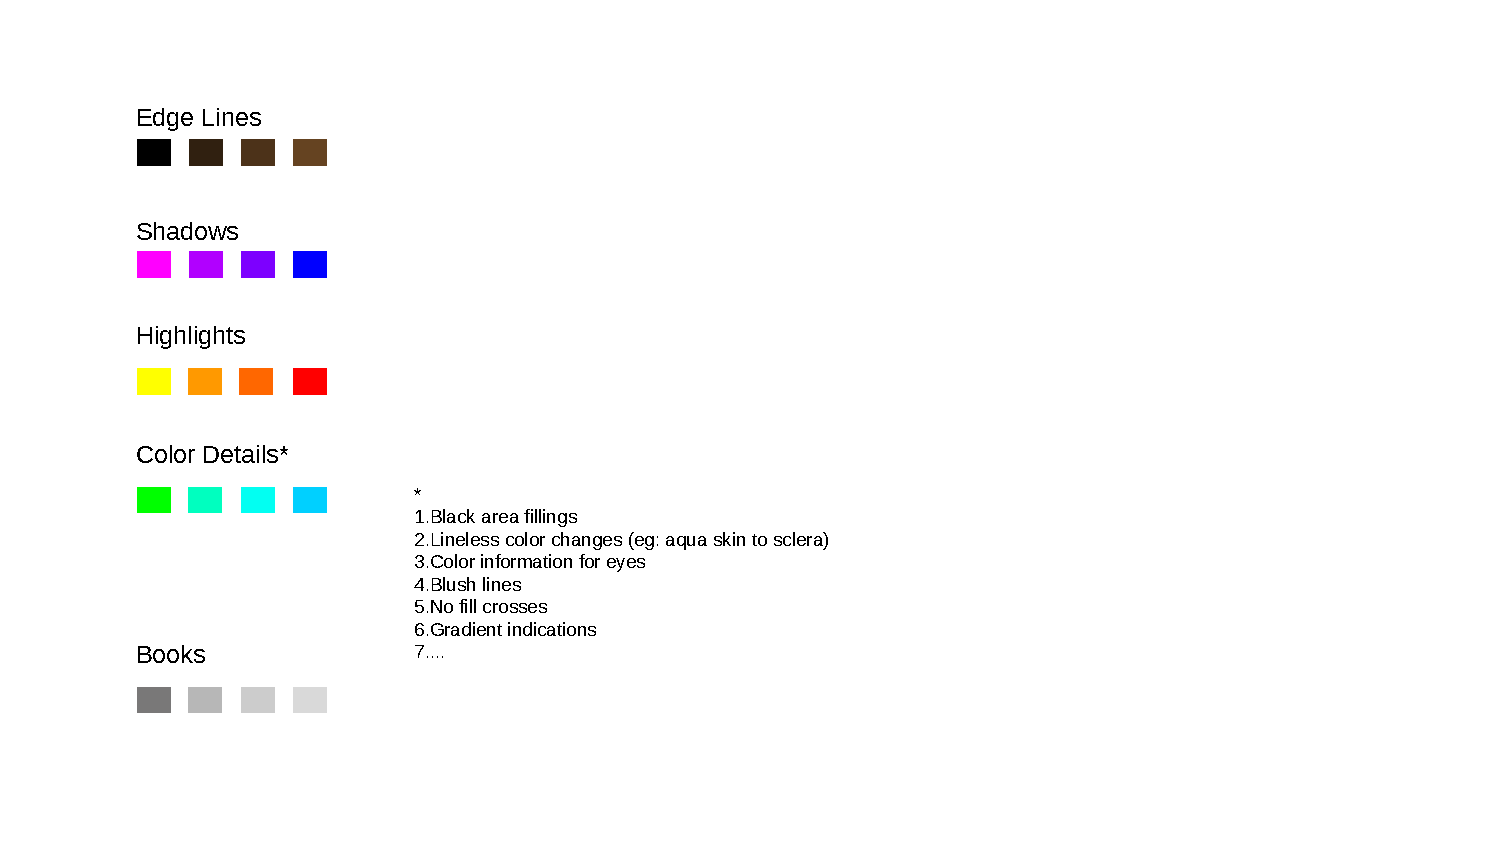
\includegraphics{graphics/Douga-Color-Schema.pdf}
    \caption{Our proposed standardized keyframe color schema, which is used in the dataset \citep{Kugler-2021}.}
    \label{fig:bg.color-schema}
\end{figure}

Clean frames can be considered a type of line art, specifically defined by the following features.

\begin{itemize}
    \item Constant stroke width: Clean frames are drawn using mostly quadratic and cubic bezier curves with a constant stroke width. While line art usually uses variable stroke widths, this is not a common style for limited animation, specifically in Japanese productions. 
    \item High number of curves:  On average, the amount of curves per image over 1000 (see \Cref{subsec:dataset.stats}), which is significantly more than the amount of curves used for simple line art that is often the target for automatic vectorization (such as doodles, fonts or cartoons).
    \item Semantically meaningful colors: The color of each curve carries semantic meaning, namely as indication for succeeding steps in the animation pipeline. There is no industry-standard for the color scheme, with studios mostly opting to use their proprietary schemes. The scheme used by example images in this work (all provided by Tonari Animation) is defined in \Cref{fig:bg.color-schema}. It can be observed in \Cref{fig:douga.example}. For example, note how the regions enclosed by blue lines are colored darker than the ones enclosed by red lines.
    \item Exact boundaries: In order to speed up the colorization step of the production workflow, it is necessary to ensure that all color regions are sufficiently enclosed by curves. This way, coloring can be trivially accomplished using bucket filling.
\end{itemize}

Even if clean frames are drawn as vector images, they might sometimes only be available in raster format. This could be the case of older clean frames, different studios working on different stages of the workflow or if it is necessary to export the image from the drawing program to another program. In this case, they need to be manually retraced before inbetweens are created, which can take around an hour. Hence, there is a need to have an automatic way of vectorizing them.

\begin{figure}[h]
    \centering
    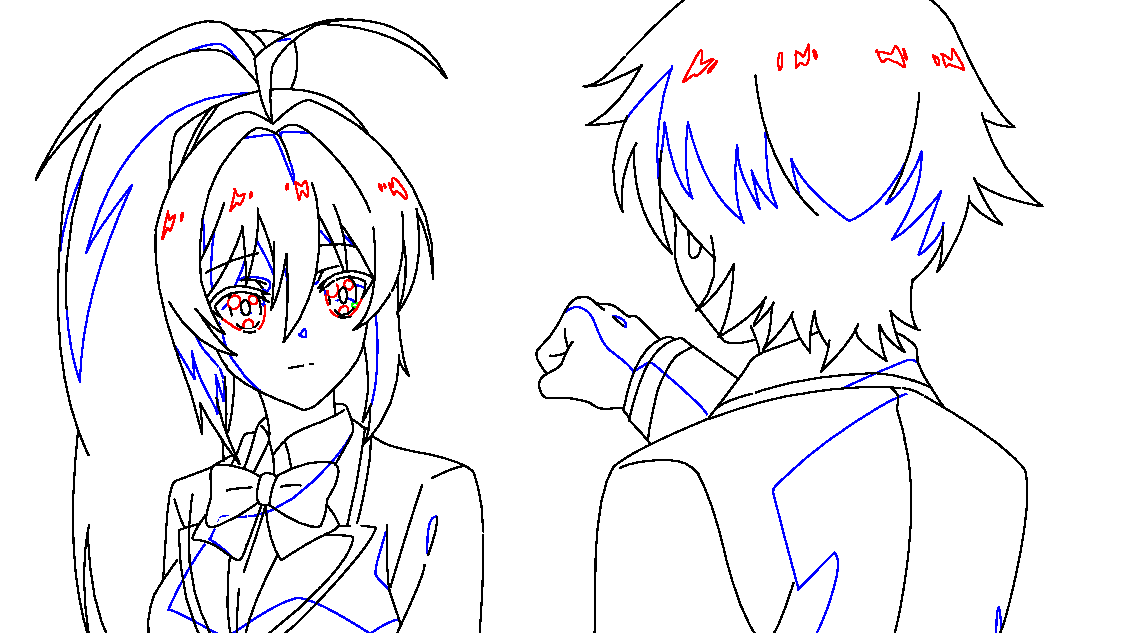
\includegraphics[width=\textwidth]{graphics/douga/39.pdf}
    \caption{The essential information of a clean animation keyframe. In essence, \Cref{fig:douga.example.clean} with all filled color regions removed.}
    \label{fig:clean-frame-vec}
\end{figure}

The objective of this work is to create an automatic way of vectorizing clean frames. For the vectorization, it is not necessary to handle the filled color regions, since those can be easily restored using pre- or post-processing and, failing that, can be trivially added manually. The essential part are the lines and curves themselves, as shown in \Cref{fig:clean-frame-vec}. %Furthermore, it is not necessary for the algorithm itself to restore curves in their correct color, since the image can easily be split automatically according to the color. Then, the vectorization algorithm can be applied on each of the resulting partial images. Afterwards, the partial results can be trivially colored and merged.

Finally, in order for the vectorization method to be practically suitable, it is important that the result minimizes the amount of manual fixing required. Hence, it is more important that the restored lines are correct, even at the expense of not all lines in the input image being covered.

\section{Deep Learning}
\label{sec:bg.dl}

When attempting to tackle a task computationally, it is common to explicitly define an algorithm that solves the task in a structured way with manually set parameters. In practice, this approach is often unfeasible for complex tasks with high-dimensional data, such as image generation or speech recognition. A different approach is \emph{machine learning}, i.e., to assemble a dataset of correct inputs and outputs and defining an algorithm which exploits statistical correlations in the dataset to fit a model that generalizes to data outside of this dataset. \emph{Deep learning} is a subset of machine learning that has gained traction in recent years due to practical successes \citep{DBLP:conf/cvpr/CiresanMS12,DBLP:conf/nips/KrizhevskySH12, DBLP:journals/nature/SilverHMGSDSAPL16,DBLP:conf/naacl/DevlinCLT19,DBLP:conf/nips/BrownMRSKDNSSAA20,DBLP:conf/cvpr/RombachBLEO22,DBLP:journals/corr/abs-2203-02155}.

The basis of deep learning are \emph{neural networks} \citep{Rosenblatt58theperceptron}, which are explained in \Cref{subsec:bg.nn}. Different ways of formulating objectives for and measuring neural networks are explored in \Cref{subsec:bg.losses}. \Cref{subsec:bg.cnn} describes \glspl{cnn} \citep{DBLP:journals/pr/FukushimaM82,10.1162/neco.1989.1.4.541}, which are a type of neural networks suited for spatial data such as raster images. The equivalent for sequential data, \glspl{rnn} \citep{Rumelhart1986}, are detailed in \Cref{subsec:bg.rnn}. The Transformer architecture \citep{DBLP:conf/nips/VaswaniSPUJGKP17,schmidhuber1992learning}, a recently developed model architecture attempting to combine the advantages of \glspl{cnn} and \glspl{rnn} is introduced in \Cref{subsec:bg.tf}. \Cref{subsec:bg.vae} describes a flexible framework for generative models called encoder-decoder framework \citep{DBLP:conf/nips/SutskeverVL14,FITPT283}.


\subsection{Neural Networks}
\label{subsec:bg.nn}

\begin{figure}[h]
\centering
\begin{tikzpicture}
    \node[circle, draw, fill=lightgray] (x0) at (0,0.5) {$x_0$};
    \node[circle, draw, fill=lightgray] (x1) at (0,1.5) {$x_1$};
    \node[circle, draw, fill=lightgray] (x2) at (0,2.5) {$x_2$};
    \node[circle, draw] (h0) at (4,0) {$h_0$};
    \node[circle, draw] (h1) at (4,1) {$h_1$};
    \node[circle, draw] (h2) at (4,2) {$h_2$};
    \node[circle, draw] (h3) at (4,3) {$h_3$};
    \node[circle, draw, fill=gray] (o0) at (8,1) {$o_0$};
    \node[circle, draw, fill=gray] (o1) at (8,2) {$o_1$};
    \draw [->] (x0) to (h0);
    \draw [->] (x0) to (h1);
    \draw [->] (x0) to (h2);
    \draw [->] (x0) to (h3);
    \draw [->] (x1) to (h0);
    \draw [->] (x1) to (h1);
    \draw [->] (x1) to (h2);
    \draw [->] (x1) to (h3);
    \draw [->] (x2) to (h0);
    \draw [->] (x2) to (h1);
    \draw [->] (x2) to (h2);
    \draw [->] (x2) to (h3);
    \draw [->] (h0) to (o0);
    \draw [->] (h0) to (o1);
    \draw [->] (h1) to (o0);
    \draw [->] (h1) to (o1);
    \draw [->] (h2) to (o0);
    \draw [->] (h2) to (o1);
    \draw [->] (h3) to (o0);
    \draw [->] (h3) to (o1);
    \node[draw, above=of x2, fill=lightgray] {input};
    \node[draw, above=of h3] {hidden};
    \node[draw, above=of o1, fill=gray] {output};
    \node at (0,-1) {$\textbf{x}$};
    \node at (2,-1) {$\boldsymbol{\theta}_{in}$};
    \node at (4,-1) {$\textbf{x}^T\boldsymbol{\theta}_{in}$};
    \node at (6,-1) {$\boldsymbol{\theta}_{h}$};
    \node at (8,-1) {$f_a(\textbf{x}^T\boldsymbol{\theta}_{in})\boldsymbol{\theta}_{h}$};
\end{tikzpicture}
    \caption{Architecture of a \gls{mlp}. Circles of same color represent the variables within a layer, while the connections between circles indicates weights. The mathematical representation is given below.}
    \label{fig:mlp}
\end{figure}

Consider a set of input data $\textbf{x}\in\mathbb{R}^m$ and a set of outputs $\textbf{y}\in\mathbb{R}^l$ of unspecified dimensions, which are related by the ground truth function $F(\textbf{x})=\textbf{y}, F: \mathbb{R}^m \rightarrow \mathbb{R}^l$. In the context of \emph{machine learning}, $\textbf{x}$ can be referred to as \emph{predictors} and $\textbf{y}$ as the \emph{response} or \emph{label}. For example, in the case of binary image classification the predictor could be a sequence of the color values of all pixels in an image, while the response could be a dichotomous variable indicating whether the image is part of the positive class. The objective of a machine learning algorithm is to fit a model $f$ that approximates $F$ using freely changeable (or, \emph{learnable}) parameters $\boldsymbol{\theta}$, i.e., $f(\textbf{x};\boldsymbol{\theta})\approx F(\textbf{x})$.

Neural networks \citep{Rosenblatt58theperceptron} can be viewed as special, nonlinear case of the approximation $f$. Specifically, a neural network consists of three types of layers:
\begin{itemize}
	\item One input layer $\textbf{x}$
    \item $n$ hidden layers and
	\item one output layer \textbf{o}
\end{itemize}

Intuitively, each hidden layer learns to detect important features of the preceding layer. These features are then used in the last layer - the output layer - to compute the relevant, task dependent outcome.

The  standard feedforward neural network, the \gls{mlp}, is depicted in \Cref{fig:mlp}. Note that \Cref{fig:mlp} depicts a neural network with only one hidden layer. Theoretically, this 1-layered \gls{mlp} is able to approximate any function \citep{DBLP:journals/nn/HornikSW89,DBLP:journals/mcss/Cybenko89}. However, in practice, it has been shown that neural networks that consist of many hidden layers perform better on complex functions \citep{DBLP:journals/tc/Amari67,DBLP:conf/icml/SafranS17,DBLP:journals/nn/PetersenV18}. The amount of hidden layers is also referred to as the \emph{depth} of the neural network, leading to the term \emph{deep learning}  \citep{DBLP:conf/aaai/Dechter86,DBLP:journals/tnn/ChenKKH01a}.

In the \gls{mlp} architecture, each hidden layer consists of a predetermined size $k$ of nodes. Every node is connected to all nodes of the preceding layer (hence also called \emph{fully connected}). Each of these connections is assigned a learnable weight $\theta$. Thus, the value of each node is the weighted sum of all nodes of the preceding layer. Therefore, each layer in a neural network can be described as inner product $\textbf{h}=\textbf{x}^T \boldsymbol{\theta}$, where $\textbf{x}$ is the vector of nodes of the preceding layer and $\boldsymbol{\theta}\in \mathbb{R}^{k\times|\textbf{x}|}$ is a matrix, where $\boldsymbol{\theta}_i \forall i \in [0,k]$ is a vector of weights for one node. For brevity, the bias term is omitted. Intuitively, each node is a specific \emph{representation} of the preceding layer which assigns a certain importance (i.e., weight) to every node of the preceding layer.

After the node values of the hidden layer are computed, an \emph{activation function} $\phi(x)$ is applied on them. Early \glspl{mlp} were inspired by biological neural networks and used the sigmoid activation function defined in \Cref{eq:sigmoid}. This function is depicted in \Cref{fig:activationfunctions.sigmoid}. A similar activation function is the tanh activation function defined in \Cref{eq:tanh} and depicted in \Cref{fig:activationfunctions.tanh}. Contemporary neural networks mainly use the \gls{relu} activation function \citep{Nair:2010:RLU:3104322.3104425} defined in \Cref{eq:relu} and depicted in \Cref{fig:activationfunctions.relu}. 

\begin{equation}
\label{eq:sigmoid}
\sigma(x)=1/(1+\exp(-x))
\end{equation}

\begin{equation}
\label{eq:tanh}
\tanh(x)={\frac {\sinh(x)}{\cosh(x)}}={\frac {e^{x}-e^{-x}}{e^{x}+e^{-x}}}
\end{equation}

\begin{equation}
\label{eq:relu}
\text{relu}(x)=\max(0,x)
\end{equation}

\begin{figure}
\centering
    \begin{subfigure}[b]{0.3\textwidth}
        \begin{tikzpicture}[scale=0.6]
            \begin{axis}
                \addplot[domain=-10:10, blue, ultra thick] {1/(1+exp(-x))};
            \end{axis}
        \end{tikzpicture}
        \caption{Sigmoid function.}
        \label{fig:activationfunctions.sigmoid}
    \end{subfigure}
    \hfill
    \begin{subfigure}[b]{0.3\textwidth}
        \begin{tikzpicture}[scale=0.6]
            \begin{axis}
                \addplot[domain=-10:10, blue, ultra thick] {(e^(x)-e^(-x))/(e^(x)+e^(-x))};
            \end{axis}
        \end{tikzpicture}
        \caption{Tanh activation function.}
        \label{fig:activationfunctions.tanh}
    \end{subfigure}
    \hfill
    \begin{subfigure}[b]{0.3\textwidth}
        \begin{tikzpicture}[scale=0.6]
            \begin{axis}
                \addplot[domain=-10:10, blue, ultra thick] {max(0,x)};
            \end{axis}
        \end{tikzpicture}
        \caption{\gls{relu} activation function.}
        \label{fig:activationfunctions.relu}
    \end{subfigure}
    \caption{Graphs depicting activation functions.}
    \label{fig:activationfunctions}
\end{figure}

The output of each hidden layer is thus $\phi(\textbf{h})=\phi(\textbf{x}^T \boldsymbol{\theta})$. Notice that $\phi$ serves as nonlinearity. If $\phi$ was not used, the output of an $n$-layered neural network could be computed using $\textbf{o} = \textbf{x}^T \prod_{i=0}^{n}\boldsymbol{\theta}_i=\textbf{x}^T \boldsymbol{\theta}$. This is equivalent to the multiple linear regression model $\textbf{y}=\textbf{x}^T \boldsymbol{\beta} + \boldsymbol{\epsilon}$.

With the activation function $\phi(x)$, a two-layered \gls{mlp} is defined by \Cref{eq:mlp.2l}.

\begin{equation}
\label{eq:mlp.2l}
	\textbf{o} = \phi(\phi(\textbf{x}^T \boldsymbol{\theta}_{\text{in}})\boldsymbol{\theta}_{\text{h}})
\end{equation}

In \Cref{eq:mlp.2l} $\boldsymbol{\theta}_{\text{in}}$ are the connection weights between the input and the hidden layer and $\boldsymbol{\theta}_{\text{h}}$ are the connection weights between the hidden and the output layer.

\subsubsection{Optimization}
\label{subsec:bg.nn.optim}
In order to approximate the ground truth function $F(\textbf{x})$ using the model $f(\textbf{x};\boldsymbol{\theta})$, the optimal parameters $\boldsymbol{\theta}^\star$ have to be found. In machine learning parlance, this is referred to as \emph{fitting}, or \emph{training} the model. In the case of neural networks, this means finding the optimal parameters $\boldsymbol{\theta}^\star_i$ for each hidden layer, such that $f(\textbf{x}; \boldsymbol{\theta}^\star) \approx F(\textbf{x})$. Historically, fitting neural networks often failed to converge to optimal parameters \citep{perceptrons}. However, this changed with the introduction of the backpropagation algorithm (also referred to as reverse-mode differentiation) \citep{Dreyfus_1962, linnainmaa}, which made it possible to efficiently train neural networks.

The first step in optimization is \emph{weight initialization}, i.e., to initialize the learnable parameters $\boldsymbol{\theta}_i$ with random numbers. Next, the output of the neural network is computed as $\textbf{o}=f(\textbf{x}; \boldsymbol{\theta})$. In order to evaluate the output of the network, a \emph{loss function} is defined as $L(\textbf{o},\textbf{y})$. $L$ calculates the error between $\textbf{o}$ and the ground truth $\textbf{y}$. It is important to choose a proper loss function fitting the specific task. A simple loss function sometimes used in image generation is the mean squared error, or $L^2$ distance, defined by \Cref{eq:mse}.

\begin{equation}
    \label{eq:mse}
    L^2(\textbf{o}, \textbf{y}) = \frac{\sum_{i=1}^{|\textbf{o}|} (o_i - y_i)^2}{|\mathbf{o}|}
\end{equation}

Using the \gls{sgd} algorithm, the loss function $L$ can be used to \emph{guide} the training process towards optimal parameters. This is done by computing the gradients $\partial L / \partial \boldsymbol{\theta}_i$ for each weight parameter using backpropagation. These gradients indicate how the loss $L$ changes when $\boldsymbol{\theta}_i$ is increased by an infinitesimal amount. As the loss function needs to be \emph{minimized}, the parameters are updated using the \gls{sgd} update step defined by \Cref{eq:sgd}.

\begin{equation}
\label{eq:sgd}
        \boldsymbol{\theta}_i = \boldsymbol{\theta}_i - \eta \frac {\partial L} {\partial \boldsymbol{\theta}_i}
\end{equation}

$\eta$ in \Cref{eq:sgd} is a hyperparameter called \emph{learning rate} or \emph{step size}. It controls the magnitude of the weight parameter updates and is often a small positive number, as higher numbers quickly lead to exploding or vanishing gradients \citep{hochreiterdipl}.

The \gls{sgd} update step, i.e., computing the outputs and changing the parameters is repeated until a set of parameters that results in a sufficiently small loss is found. In recent times, several enhancements to the \gls{sgd} algorithm were proposed. Most of them are \emph{adaptive} optimization algorithms, i.e., they adapt the learning rate $\eta$ according to the previous gradients or parameter updates. Chief among them are Adam \citep{DBLP:journals/corr/KingmaB14}, AdamW \citep{DBLP:conf/iclr/LoshchilovH19} and RMSprop \citep{rmsprop}. While it is still unproven that these optimization algorithms are strictly better than \gls{sgd} \citep{DBLP:conf/icml/HardtRS16, NIPS2017_7003}, they do perform better on some tasks and model architectures \citep{DBLP:conf/emnlp/LiuLGCH20,DBLP:conf/nips/Anil0KS19}.

For the optimization process to work, it is crucial that the gradients required for the update step $\partial L / \partial \boldsymbol{\theta}_i$ can actually be computed. This means that the loss function $L(\textbf{o},\mathbf{y})$ needs to be \emph{differentiable}, i.e., there must be a derivative at all points in its domain. Since $\textbf{o}=f(\textbf{x}; \boldsymbol{\theta})$ and since the gradients are computed directly with respect to individual $\boldsymbol{\theta}_i\in\boldsymbol{\theta}$, it follows that the model $f$ itself also needs to be differentiable. As an aside, the \gls{relu} activation function defined in \Cref{eq:relu} is actually not differentiable at $x=0$. In order to enable it to be used in the model anyways, the derivative at $x=0$ is arbitrarily set to $0$ ($\text{relu}'(0)=0$).

\subsubsection{Regularization}
\label{subsec:bg.nn.reg}

A common occurrence while training neural networks is \emph{overfitting}, i.e., finding parameters $\boldsymbol{\theta}$ that closely fit the data used to train the network, but do not generalize to unseen data. In order to prevent this, several regularization schemes are employed.

\paragraph{Model and Dataset Size}
In general, the larger a model is (i.e., the more freely changeable parameters $\theta$ it contains) in relation to the dataset size, the easier it is to overfit. Therefore, an important design decision to reduce overfitting is to either reduce the model parameters to the smallest capacity required to converge or to increase the dataset size.

\paragraph{Weight initialization}
Weight initialization is an important decision for the training process, as wrongly initialized neural networks do not converge to a sufficient result \citep{pmlr-v9-glorot10a,Sutskever:2013:IIM:3042817.3043064}. Therefore, one often draws the initial weights of each hidden layer from a Gaussian distribution $\boldsymbol{\theta}_i \sim \mathcal{N}(0,1)$ and scales the variance with a constant. One commonly used method is Xavier initialization \citep{pmlr-v9-glorot10a}, which scales the random numbers by $2/(n_{\text{pre}} + n_{\text{next}})$, where $n_{\text{pre}}$ is the number of nodes of the preceding layer and $n_{\text{next}}$ is the number of nodes in the succeeding layer. Another initialization scheme specifically designed for \gls{relu} neural networks is He initialization \citep{He:2015:DDR:2919332.2919814} with a scale factor of $\sqrt{2/n}$, where $n$ is the number of nodes of each hidden layer.

\paragraph{Batch normalization}
\label{subsec:bg.nn.batchnorm}
Neural networks are normally fitted by processing subsets of the training dataset - \emph{batches} - in parallel. This is primarily done to utilize the nature of \glspl{gpu} in order to speed up the training process. However, it is also possible to use batch statistics to normalize individual observations with respect to the batch. This \emph{batch normalization} \citep{pmlr-v37-ioffe15} ensures that batches are normally distributed, which might improve the stability of the training process. The authors claim that internal covariate shift - i.e., differing distributions of intermediate layer outputs - are detrimental to convergence. However, there exist alternative explanations for how batch normalization actually brings about its regularizing effects in practise \citep{NEURIPS2018_905056c1, DBLP:conf/iclr/YangPRSS19, DBLP:conf/aistats/KohlerDLHZN19}.

More specifically, given a batch $\textbf{x}_B \subset \textbf{x}$, each observation $x_i \in \textbf{x}_B$ is centered using the batch mean $\mu_{B}={\frac {1}{m}}\sum _{i=1}^{m}x_i$ and scaled by the batch variance $\sigma _{B}^{2}={\frac {1}{m}}\sum _{i=1}^{m}(x_i-\mu_{B})^{2}$ as given by \Cref{eq:batchnorm}. In this equation, $k$ denotes the dimension, since batch normalization is applied per-dimension.

\begin{equation}
    \label{eq:batchnorm}
    \hat {x}_{i}^{(k)}={\frac {x_{i}^{(k)}-\mu _{B}^{(k)}}{\sqrt {\left(\sigma _{B}^{(k)}\right)^{2}+\epsilon }}}
\end{equation}

\paragraph{Dropout}
Another way to regularize neural networks and reduce overfitting is to randomly set individual nodes in hidden layers to 0. This technique is called \emph{dropout} \citep{DBLP:journals/corr/abs-1207-0580} and makes the model more robust with respect to individual nodes and their connection weights, since it can not rely on the node value being present.

Dropout is mainly applied while fitting the model. Consider the hidden layer $\textbf{h}=\textbf{h}_{-1}\boldsymbol{\theta}$. After computing the hidden layer nodes $\textbf{h}$ using the preceding layer $\textbf{h}_{-1}$  and the connection weights $\boldsymbol{\theta}$, each node $h \in \textbf{h}$ is independently set to 0 with probability $p$ (it is common to set $p=0.5$). Since this is independently done for every step of the optimization process, different nodes will be "dropped" at each step. Hence, in order to maximize the optimization objective, the connection weights have to be fitted in a way that is robust to a share $p$ of the nodes randomly being dropped (and thereby a share $p$ of the weights not contributing to the output).

\subsection{Metrics and Losses}
\label{subsec:bg.losses}
Recall that a machine learning model $f(\mathbf{x};\boldsymbol{\theta})=\mathbf{o}$ approximates a ground truth function $F(\textbf{x})=\textbf{y}$ by being fitted to an input dataset $(\mathbf{x},\mathbf{y})$ in order to produce outputs $\mathbf{o}$ that fit the ground truth output (or, response) $\mathbf{y}$. It follows, that there is a need for a single numerical value to measure this fit. There are two ways this value is calculated and used in relation to a machine learning model: firstly, to evaluate the model after it has been trained using \emph{metrics} (often against other models or baselines) and secondly, in order to guide the training process using \emph{loss functions}. This section introduces these related concepts.

\subsubsection{Classification}
\label{subsubsec:classification}
Since metrics and losses formulate the objective, they depend on the task of the model. Machine learning tasks can be roughly divided into two categories by the nature of the response $\mathbf{y}$. While in regression tasks, $\mathbf{y}$ is continuous, in classification tasks $\mathbf{y}$ is discrete.

Regression does not impose strict assumptions on $\mathbf{y}$ is therefore the standard case introduced in \Cref{subsec:bg.nn}. An important image-related task that roughly falls into this category is image generation, i.e., to generate output images $\mathbf{o}$ that look similar to the ground truth $\mathbf{y}$.

On the other hand, classification has more strict assumptions on $\mathbf{y}$. The task is to assign to an input $\mathbf{x}$ a predefined class out of $S$ classes. Since machine learning models operate on vectors, the class in the ground truth is represented as a vector $\mathbf{y}\in\mathbb{R}^S$, where each element $y_i\in\mathbf{y}$ is an indicator of the class $i\in[1,S]$. If the input is assigned class $s$, $y_s=1$ and $y_j=0\forall j\in[1,S]$ except $j=s$. Appropriately, the output of the model $\mathbf{o}$ has the same structure as the ground truth $\mathbf{y}$, except it usually consists of continuous class \emph{probabilities} instead of categorical class indicators, i.e., whereas $y_i\in\{0,1\}$, $o_i\in[0,1]$. In the case of binary classification, i.e., if $S=2$, the two class probabilities are exactly the inversion of each other and can be reduced to a single probability, i.e., in this case the class is represented by a single number.

There are image-related tasks that can be framed as classification tasks. Consider the case of image segmentation, which has the objective of partitioning an image into multiple segments, where each segment belongs to one of multiple classes. All regions of a class share certain task-dependent characteristics. \Cref{fig:segmentation} shows an example of an image segmentation task. This example depicts a binary image segmentation task where the image has to be segmented into two classes: segments that correspond to circles and the rest.

\begin{figure}
    \centering
    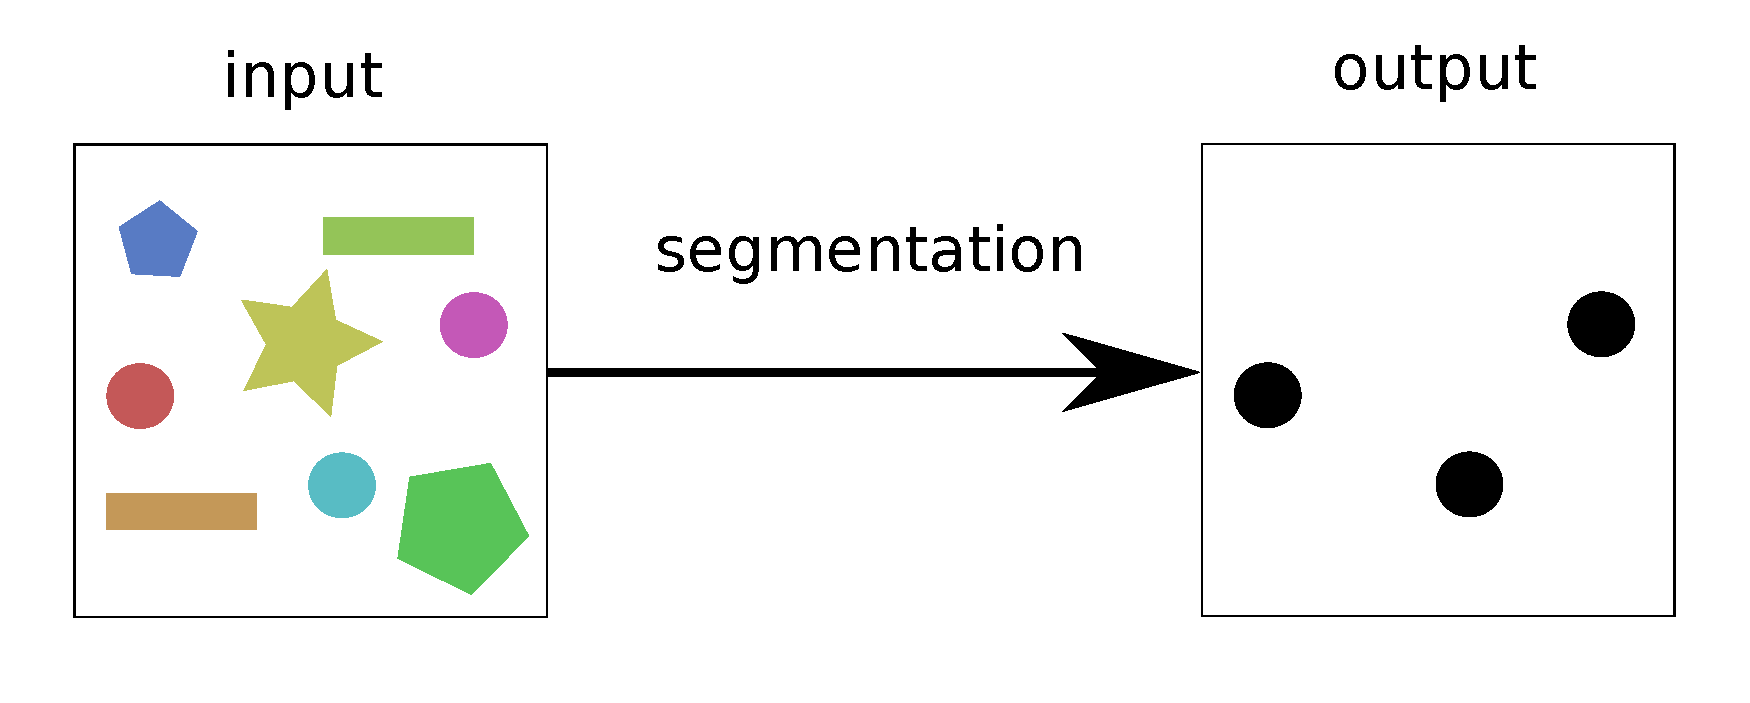
\includegraphics[width=\textwidth]{graphics/segmentation.pdf}
    \caption{An example of image segmentation, where the circles in the image have to be segmented.}
    \label{fig:segmentation}
\end{figure}

In other words, the output of a segmentation model assigns a class to each pixel of the input image. Given an input image $\mathbf{x}\in\mathbb{R}^{W\times H\times C}$ of width $W$, height $H$ and $C$ color values per pixel, the output is $\mathbf{o}\in\mathbb{R}^{W\times H\times S}$, where $S$ is the number of classes. In detail, each pixel $\mathbf{x}_{i,j}\in\mathbf{x}$ at location $(i,j)$ in the input image $\mathbf{x}$ is assigned a vector $\mathbf{o}_{i,j}\in\mathbf{o}$ of length $|\mathbf{o}_{i,j}|=S$, where the element $o_s\in\mathbf{o}_{i,j}$ indicates the probability that the pixel belongs to class $s$ $\forall s\in[1,S]$. Furthermore, it holds that $o_s\in[0,1] \forall s$ and $\sum_{k=0}^{|\mathbf{o}|} o_k=1$. In the special case of $S=2$, the class dimension of the output vector can be interpreted as a monochrome color model and the output can be visualized as an image in which the positive class is indicated as black and the negative class is indicated as white. An example of this is shown in \Cref{fig:binaryseg}. Note that clean animation keyframes can be seen as image segmentation output of corresponding final animation frames (see \Cref{fig:douga.example}).

\begin{figure}
    \centering
    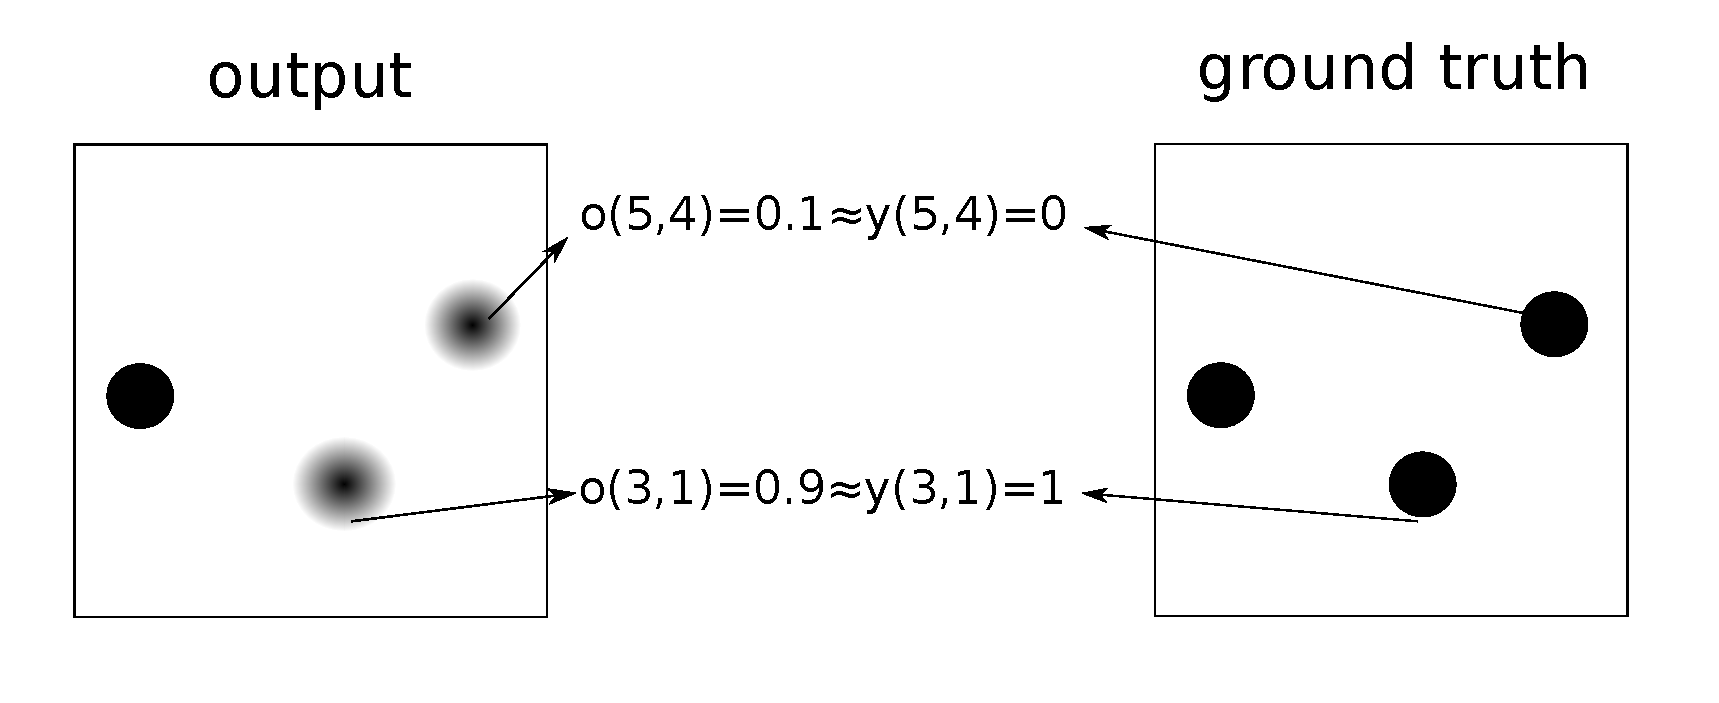
\includegraphics[width=\textwidth]{graphics/binaryseg.pdf}
    \caption{An example of binary image segmentation using binary classification. On the left, an output of a model that has not yet converged is visualized as a monochrome image. The ground truth data is displayed on the right. Note the continuous class probabilities being used in the model output.}
    \label{fig:binaryseg}
\end{figure}

Keep in mind that image segmentation is often associated with class imbalance, i.e., under-representation of a class in the training dataset, which has to be considered by metrics and loss functions.



\subsubsection{Metrics}
\label{subsubsec:metrics}
It is important to evaluate how good a model $f$ performs. This is measured using metric that computes the difference between the model output $\mathbf{o}$ and the ground truth $\mathbf{y}$. However, notice that $\mathbf{y}$ is used to both fit the model and evaluate it. Therefore, a model that trivially memorizes the input and output data would attain a perfect evaluation score. However, this model would not generalize to unseen data. Since the primary aim of a model is to be applied to unseen data, it is conductive not to evaluate the model on these instead of the data it has been fitted to.

In order to attain evaluation on unseen data, the principal training scheme is splitting the available dataset of input data $\mathbf{x}$ and labels $\mathbf{y}$ into a training dataset $\mathbf{x}_\text{train} \subset \mathbf{x}, \mathbf{y}_\text{train} \subset \mathbf{y}$ and a test dataset $\mathbf{x}_\text{test} \subset \mathbf{x}, \mathbf{y}_\text{test} \subset \mathbf{y}$, where $\mathbf{x}_\text{train} \cap \mathbf{x}_\text{test} = \varnothing$ and $\mathbf{y}_\text{train} \cap \mathbf{y}_\text{test} = \varnothing$. The training dataset is used solely to fit the model, while the test dataset is used to evaluate the model. Special care needs to be taken such that there is no information leak from the test dataset into the training dataset.

Specifically, the metric functions introduced below are applied on the ground truth of the test dataset $\mathbf{y}_\text{test}$ and the model output $\mathbf{o}=f(\textbf{x}_\text{test};\boldsymbol{\theta})$, where $\boldsymbol{\theta}$ has been fitted using the training dataset $\mathbf{x}_\text{train}, \mathbf{y}_\text{train}$. The metrics are introduced for regression and classification models, respectively.

\paragraph{Regression}
This section introduces two common metrics that can be used to measure models trained for regression tasks. Let $\mathbf{o}$ and $\mathbf{y}$ be in Euclidean space, then the ordinary distance between them $\mathbf{y}-\mathbf{o}$ (i.e., the error) can be directly calculated and used as metric. However, by simply computing the subtraction, large negative distances would actually contribute to minimizing the error. There are two common metrics which prevent this. While the \gls{mae} (also referred to as $L^1$ distance) as defined in \Cref{eq:mae} uses the absolute of the error, the \gls{mse} (or, $L^2$ distance) as defined in \Cref{eq:mse} uses the square of the error. These metrics can be used as a simple way to calculate the difference between two images.

\begin{equation}
\label{eq:mae}
    L^1(\textbf{o}, \textbf{y}) = \frac{\sum_{i=1}^{|\textbf{o}|} |o_i - y_i|}{|\mathbf{o}|}
\end{equation}

\paragraph{Classification}
This section introduces metrics for binary classification models, which are used for the binary image segmentation task explained in \Cref{subsubsec:classification}. Binary classifiers are often evaluated by first computing their confusion matrix, which counts all possible configurations of class assignments per input observation (i.e., pixel in image segmentation). It is displayed in \Cref{tab:confusion}, where $TP$ refers to the true positives, i.e., the amount of observations to which both the model and the ground truth assign the positive class, $FP$ refers to the false positives, i.e., the amount of observations to which the model assigns the positive and the ground truth assigns the negative class and $FN$ refers to the false negatives, i.e., the amount of observations to which the model assigns the negative and the ground truth assigns the positive class.

\begin{table}[h]
	\caption{Confusion matrix for a binary classifier.}
	\label{tab:confusion}
	\begin{center}
		\begin{tabular}{c|cc}
			 & $y=1$ & $y=0$  \\
			\hline
			$o=1$ & \glspl{tp} & \glspl{fp} \\
			$o=0$ & \glspl{fn} & \glspl{tn} \\
		\end{tabular}
	\end{center}
\end{table}

As confusion matrices consists of four numbers, they somehow need to be reduced to a single number. There are different ways of doing that, which are described below.

%\subparagraph{Accuracy}
An easy metric that is commonly used is accuracy as defined in \Cref{eq:acc}. Notice that $ACC\in[0,1]$. However, this metric does not take into account the proportion of positive class observations over negative class observations in the dataset. Therefore, in the case of class imbalance, the metric is biased towards the over-represented class.

\begin{equation}
\label{eq:acc}
	ACC = \frac{TP + TN}{TP + FP + TN + FN}
\end{equation}

%\subparagraph{Intersection-over-Union}
One strategy of combating class imbalance in binary classification problems is to consider the intersection between the output and the ground truth. This is done using the \gls{iou} \citep{gilbert1884,https://doi.org/10.1111/j.1469-8137.1912.tb05611.x,tanimoto1958elementary} (also referred to as Jaccard index), which is defined in \Cref{eq:iou}. Notice that $J\in[0,1]$. As the name suggests, \gls{iou} divides the intersection, i.e., the amount of observations to which both the output and the ground truth assign the positive class by their union. It can be seen in \Cref{eq:iou} that only the amount of true positives increases the IoU metric. Hence, even if the negative class is over-represented, it does not affect the metric.

\begin{equation}
    \label{eq:iou}
    J = \frac{TP}{TP+FP+FN}
\end{equation}

%\subparagraph{Dice}
Another metric that is closely related to the \gls{iou} is the dice coefficient \citep{https://doi.org/10.2307/1932409,sorensen1948method} (also referred to as Sørensen index or $F_1$ score), which is defined in \Cref{eq:dice.coef}. Notice that $S\in[0,1]$. It differs from the \gls{iou} by multiplying the true positives by 2. This way, the true positives contribute exactly the same as the false positives and false negatives together to the denominator. Aside from that, it is identical to the \gls{iou} and related by $S=2J/(1+J)$. Hence, the \gls{iou} and dice coefficient are positively correlated.

\begin{equation}
\label{eq:dice.coef}
    S=\frac{2TP}{2TP+FP+FN}
\end{equation}

\subsubsection{Losses}
\label{subsubsec:losses}
As explained in \Cref{subsec:bg.nn.optim}, loss functions are an integral component of the optimization process of neural networks. This section will detail important loss functions used for tasks involving raster images. A loss function $L(\mathbf{o},\mathbf{y})$ is the mathematical representation of the optimization objective (i.e., the task). It assesses the fit of the model to the training dataset by computing the numerical error between the neural network output $\mathbf{o}$ and the ground truth $\mathbf{y}$. The loss function is used to \emph{guide} the model to convergence (i.e., optimal performance). Since neural networks are optimized by adjusting the model parameters $\boldsymbol{\theta}$ using \gls{sgd}, it needs to be a continuous function, i.e., small changes of the argument should not lead to large changes of the image. This implies that the function is differentiable at all elements in its domain.

In general, it is possible to optimize neural networks using simple metrics such as accuracy (explained further in \Cref{subsubsec:metrics}). However, in most cases, there exists a loss function that encapsulates the same meaning, but satisfies the above properties, leading to better convergence performance by the model.

Again, as is the case for the above metrics, loss functions are introduced first for regression and subsequently for classification tasks.

\paragraph{Regression}
\label{p:losses.regression}

The regression metrics \gls{mae} and \gls{mse} as defined in \Cref{eq:mae,eq:mse} can be directly used as a loss functions, since they are continuous.
%\subparagraph{Huber Loss}
%\label{p:huber.loss}
However, both have their own advantages and disadvantages. Since the \gls{mse} amplifies values, it is not as robust to outliers as the \gls{mae}. On the other hand, it is smoother at values near 0. In order to combine the advantages of both losses, \citet{10.1214/aoms/1177703732} introduced the Huber loss, which is defined in \Cref{eq:huber}. A hyperparameter $\delta\in R^{+}$ serves as threshold. If the absolute error is below this threshold, the squared error is used, otherwise the absolute error is used.

\begin{equation}
\label{eq:huber}
\begin{gathered}
\text{Huber}_i(o,y)={\begin{cases}{\frac {1}{2}}(y-o)^{2}&|y-o|\leq \delta\\\delta * \left(|y-o|-{\frac {1}{2}}\delta \right)&\text{otherwise}\end{cases}}\\
\text{Huber}(\mathbf{o},\mathbf{y})=\frac{\sum_{i=0}^{|\mathbf{o}|} \text{Huber}_i(o_,y_i)}{|\mathbf{o}|}
\end{gathered}
\end{equation}


%\subparagraph{Perceptual Loss}
The \gls{mae}, \gls{mse} and Huber losses measure the similarity between images at a pixel level. However, this assumes that every pixel contributes uniformly to the similarity, which is often not the case. Furthermore, it has been posited that Euclidean losses suffer from the \emph{curse of dimensionality} \citep{DBLP:journals/sadm/ZimekSK12}, i.e., are not meaningful for high-dimensional data such as images.
%although that view has also been challenged \citep{DBLP:journals/pami/LinLRCLM22}.
A different method of measuring the similarity is to calculate the difference of high-level \emph{features} of the images. \citet{DBLP:conf/eccv/JohnsonAF16} introduce the \emph{perceptual} loss function, which implements this principle. They first process both the output and the ground truth image using a pre-trained deep neural network such as a ResNet trained on the ImageNet dataset (see \Cref{subsec:bg.cnn.arch}) to extract high level features from the ultimate hidden layer. Then, the loss function is simply the difference between these feature vectors.

\subsubsection{Classification}
Recall that binary classification tasks such as image segmentation are often associated with class imbalance, i.e., under-representation of a class in the training dataset. If this is not considered in the loss function, the optimization process often converges to the local optimum of simply ignoring this class.

\paragraph{Cross-entropy Loss}
The cross-entropy loss is a popular loss function for classification tasks. It is defined for $S$ classes in \Cref{eq:crossentropy} and is related to the softmax function defined in \Cref{eq:softmax} (see \Cref{subsec:bg.tf}). Note that $k$ is the assigned class in the ground truth, i.e., for which $y_k=1$. Intuitively, the loss function interprets the individual elements of $\textbf{o}$ as unnormalized logarithmic class probabilities and calculates their difference to the ground truth class indications $\mathbf{y}$. That is, $CE(\textbf{o},\textbf{y})$ is minimized if $o_k=1$ and $o_i=0$ $\forall i \in [1, S]$ given that $i \neq k$. \Cref{eq:crossentropy} contains the term $w_s\in[0,1]$, which weights the distance per class. The standard cross-entropy loss is unweighted, i.e., $w_s=1\forall s\in[1,S]$. In the case of class imbalance, it makes sense to balance the contribution of each class to the loss by increasing or decreasing their weight respective to their representation. In this case $w_s\neq1$ for at least one $s\in[1,S]$ and the loss is referred to as \emph{weighted} cross-entropy loss. In case of binary classification, \emph{binary} cross-entropy loss as defined in \Cref{eq:bce} can be used.

\begin{equation}
        \label{eq:crossentropy}
        CE_S(\textbf{o}, \textbf{y}) = -w_k\log \left( \frac {\exp(o_k)} { \sum_{j=1,j\neq k}^{S} \exp(o_j)}\right)
\end{equation}

\begin{equation}
    \label{eq:bce}
BCE(o,y) = CE_2(o,y)= \begin{cases} -w\log(o) &\text{if $y = 1$}\\
 -w\log (1 - o) &\text{otherwise}\end{cases}
\end{equation}

\paragraph{Focal loss}
The weighted binary cross-entropy loss defined in \Cref{eq:bce} combats class imbalance in binary image segmentation tasks by weighing predictions of the positive class over the negative class. However, \citet{DBLP:conf/iccv/LinGGHD17} proposed that weighing incorrect predictions over correct predictions leads to better results. This is implemented as a modification to the binary cross-entropy loss called \emph{focal loss}. Focal loss is defined by \Cref{eq:focal}, where $\gamma\in[0,\infty)$ is the \emph{focusing} parameter and $\alpha\in[0,\infty)$ is the \emph{balancing} parameter. While the balancing parameter $
\alpha$ adjusts the weight by which correct predictions are down-weighted, the focusing parameter $\gamma$ adjusts the rate at which correct predictions are down-weighted. Note that if $\gamma=0$ or $\alpha=0$, $FL(o,y)=BCE(o,y)$.

\begin{equation}
\label{eq:focal}
FL(o,y)=\begin{cases}  -\alpha(1-o)^\gamma \log(o) &\text{if $y = 1$}\\
 -(o)^\gamma \log(1-o) &\text{otherwise}\end{cases}
\end{equation}

\paragraph{Dice Loss}
\label{p:dice.loss}
A different strategy of combating class imbalance in binary image segmentation problems is to measure the overlap between the output and the ground truth, as is done in the \gls{iou} (see \Cref{eq:iou} and the dice coefficient (see \Cref{eq:dice.coef}). However, these functions are not continuous. \citep{DBLP:conf/3dim/MilletariNA16} introduced a differentiable version of the dice coefficient which is defined in \Cref{eq:dice}. This dice loss function is unaffected by class imbalance by design. One disadvantage is that it is not as smooth as the binary-crossentropy loss function.

\begin{equation}
\label{eq:dice}
    \text{dice}(o,y)=1-\frac{2yo+1}{y+o+1}
\end{equation}


\subsection{Convolutional Neural Networks}
\label{subsec:bg.cnn}

The \gls{mlp} architecture introduced in \Cref{subsec:bg.nn} is designed for general-purpose input data, i.e., it does not impose strict assumptions on the input data. In contrast, the \gls{cnn} architecture \citep{DBLP:journals/pr/FukushimaM82,10.1162/neco.1989.1.4.541} is designed for spatial data such as raster images.

A raster image could be represented as a flattened vector containing a sequence of color values of all pixels $\textbf{x}\in\mathbb{R}^{D}$, where $D$ is the product of the image width $W$, image height $H$, and number of color values per pixel $C$. This way, raster images can be used as input data for \glspl{mlp}. However, these input vectors quickly get very large. Consider a small raster image of width $W=224$ and height $H=224$ containing $C$ color values per pixel (with $C=3$ under the usual assumption of using the \gls{rgb} color model. The input vector representing this image would consist of $W\times H\times C=224\times224\times3=150528$ entries. Now, since the \gls{mlp} architecture consists of \emph{fully connected} layers, the nodes of the first hidden layer need to be connected to every element in the input vector. Assuming a hidden layer size of 1000, the vector of connection weights would consist of $224\times224\times3\times1000=150528000$ elements. This is disadvantageous for two reasons. First, the storage space required for the vector would be very large. Assuming that every entry is stored using a 32-bit floating point value, this would amount to a storage size of $150528000x32=602112000 \text{B} \approx 602 \text{MB}$ for one layer alone. Secondly, and more importantly, due to the sheer number of freely changeable parameters, the model is very hard to optimize and likely to overfit. 

The amount of parameters can be reduced by replacing fully connected layers with \emph{locally connected} layers, i.e., hidden layers in which nodes are not connected to all input nodes, but just to a smaller subset of input nodes. This could be done naively by just splitting the input layer into mutually exclusive subsets and connecting hidden layer nodes to a specific subset. However, in \glspl{cnn}, the locally connected layers are constructed by taking the spatial structure of raster image data into account. This is done first by arranging raster images in a 3-dimensional grid according to the image width, image height and the number of color values (also called \emph{channels}) $\textbf{x}\in\mathbb{R}^{W\times H \times C}$. Next, the assumption is made that pixels that are spatially close are related to each other. Thus, each hidden layer node is connected to a rectangular (usually square) subregion of nearby pixels in the input vector (i.e., the raster image). This subregion is also called \emph{receptive field} of the hidden layer node and is usually quite small with respect to the width and height, an example being a width and height of 3 pixels, although there are indications that larger receptive fields perform better in practice \citep{liu2021Swin,DBLP:conf/cvpr/0003MWFDX22}. It is important to note that while the receptive field is locally connected in the spatial dimensions (i.e., width and height respectively), it is fully connected along the non-spatial dimension (i.e., the channels, in this case the number of color values per pixel).

The spatial structure of input images should be preserved across locally connected hidden layers. In other words, nodes with neighbouring receptive fields should be next to each other. Hence, locally connected hidden layers are arranged as 2-dimensional grid $\textbf{h}\in\mathbb{R}^{W_h\times H_h}$, where $W_h$ is the width and $H_h$ is the height of the hidden layer. If padding is used, $W_h=W_{h-1}=W$ and $H_h=H_{h-1}=H$, i.e., the width and height remain the same across layers. Every node $n_{i,j}\in\mathbf{h}$ at position $(i,j)$ in a locally connected layer computes $n_{i,j}=\mathbf{x}^{[i:i+c,j:j+c]}\boldsymbol{\theta}_{i,j}$ where $\mathbf{x}$ is the whole input matrix, $c$ is the receptive field size (e.g. $c=3$) and $\boldsymbol{\theta}_{i,j} \in \mathbb{R}^{c\times c\times C}$ are the connection weights (i.e., parameters) of the node. Put another way, the node  computes higher-level features from the low-level input data of its receptive field. In this way, it is a differentiable feature extractor. Since it is differentiable, it can be used to \emph{learn} feature extraction using the optimization approach described in \Cref{subsec:bg.nn}. This approach is also called \emph{representation learning}. Since $\boldsymbol{\theta}_{i,j}\neq\boldsymbol{\theta}_{k,l} \forall i,j,k,l$, each node in this architecture would learn a different feature extractor. However, the feature extraction process itself should be invariant to the location of the receptive field. As an example, a potential feature extraction task could be to detect whether an object is present in the receptive field. It is clear that the object will certainly not be in the same location in every image. In this case, every node should perform this object detection on its receptive field. Therefore, all nodes need to perform the same feature extraction. This is ensured by having the weights be shared across nodes, i.e., $\boldsymbol{\theta}_{i,j}=\boldsymbol{\theta}_{k,l}=\boldsymbol{\theta} \forall i,j,k,l$. Weight sharing also drastically reduces the amount of freely changeable parameters. Since $\boldsymbol{\theta} \in \mathbb{R}^{c\times c\times C}$, such a layer requires only $C*c^2$ connection weights. Given a receptive field size of $c=3$ and number of colors per pixel $C=3$, this adds up to 27 weights, which is drastically lower than the 150528000 weights required for a fully connected layer.

\begin{equation}
\label{eq:conv}
    \textbf{o}_{i,j}=\sum_{k=0}^c\sum_{l=0}^c \textbf{w}_{k,l} \textbf{x}_{i+k,j+l}
\end{equation}

The nodes of locally connected layers with shared parameters perform a computation that is similar to discrete convolution, which is defined in \Cref{eq:conv} and visually represented in \Cref{fig:convolution}. In \Cref{eq:conv} $\textbf{o}_{i,j}$ is the element at position $(i,j)$ of the output feature map $\mathbf{o}\in\mathbb{R}^{W_o\times H_o}$ (with $W_o$ denoting the width and $H_o$ the height), $c$ is the receptive field size, $\textbf{x}_{i+k,j+l}$ is the element at position $(i+k,j+l)$ of the input map $\mathbf{x}\in\mathbb{R}^{W\times H\times C}$, and $\textbf{w}_{k,l}$ is the element at position $(k,l)$ of the kernel $\mathbf{w}\in\mathbb{R}^{c\times c\times C}$. Intuitively, the kernel is a linear transformation encoded as a matrix, which is moved across the image width-first and used to successively compute matrix multiplications with (i.e., apply a linearly transformation on) the corresponding subregions of the input matrix. In other words, the linear transformation is \emph{convolved} with the input matrix. Due to the similarity to convolution, the aforementioned locally connected layers are called \emph{convolutional} layers. The important difference is that in convolutional layers, the kernel consists of parameters that are optimized during the learning procedure, i.e., $\mathbf{w}=\boldsymbol{\theta}$.

\begin{figure}
\centering
    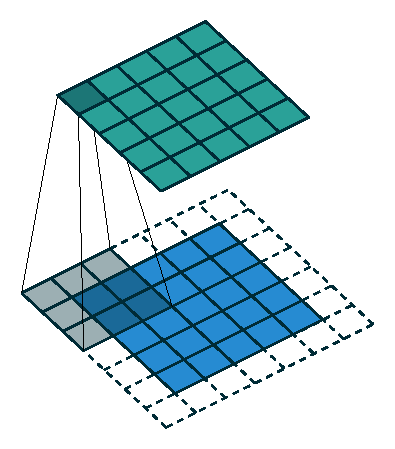
\includegraphics{graphics/same_padding_no_strides_00.pdf}
    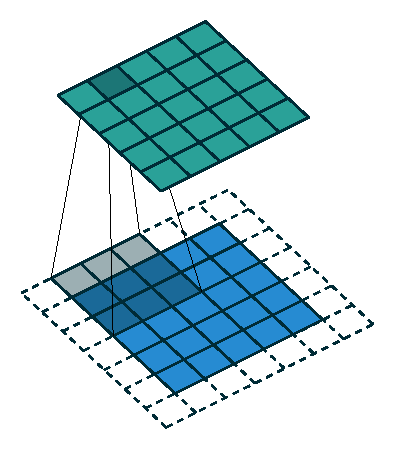
\includegraphics{graphics/same_padding_no_strides_01.pdf}
    \caption{Example of a convolution with padding to preserve width and height by \citet{dumoulin2016guide}. The left image depicts the receptive field used to compute the output element at location (1,1) in the output map. The right image depicts the receptive field used to compute the output element at location (2,1).}
    \label{fig:convolution}
\end{figure}

Convolutional layers as introduced above share their parameters across all nodes. Hence, only one feature extraction task can be performed per layer. In order to perform multiple feature extractions per layer, the layer is simply replicated multiple times along a non-spatial dimension. Recall that a convolutional layer is arranged as a 2-dimensional grid $\textbf{h}\in\mathbb{R}^{W_h\times H_h}$. This layer is now replicated $C_h$ times in order to create a 3-dimensional grid $\textbf{h}\in\mathbb{R}^{W_h\times H_h\times C_h}$. The parameters are only shared across the spatial dimesions (i.e., width and height), but not across the channel dimension. Due to this replication, given a receptive field size $c$ and input matrix channel size $C$, the parameter vector $\boldsymbol{\theta} \in \mathbb{R}^{c\times c\times C}$ extends to $\boldsymbol{\theta} \in \mathbb{R}^{c\times c\times C\times C_h}$. Hence, such a layer requires $c^2*C*C_h$ weights. Using the above example of $c=3$, $C=3$ and a reasonable $C_h=64$, this adds up to 1728 weights, which is still considerably smaller than the 150528000 weights required for a fully connected layer. Thus, by increasing the parameters along the channel dimension, this hidden layer performs $C_h$ different feature extraction tasks. Each feature map per channel dimension is also called a \emph{filter}, correspondingly, $C_h$ is referred to as the \emph{filter size}. Furthermore, the hidden layers now possess the same dimensionality as the input layer (i.e., the input image).

Note that the input layer as well as the convolutional layers are 3-dimensional matrices. Furthermore, while the convolutional layers are always locally connected along the spatial dimensions (i.e., width and height), they are fully connected along the non-spatial dimension. This makes it trivial to use the convolutional layer output as input for a succeeding convolutional layer, i.e., to stack hidden layers. Just as in \glspl{mlp}, nonlinearities are required between the layers, with the most commonly used being \gls{relu} activations. By stacking multiple convolutional layers, it is possible to perform \emph{hierarchical} feature extraction. While the first convolutional layer operates on low-level data (i.e., pixels), the succeeding layer operates on the extracted features of the first layer. Successively, layer $n$ extracts features from layer $n-1$. Thus, the local features extracted in the first layers will be used to extract increasingly global features in the last layers. Finally, global features are used for downstream tasks, such as classification or object detection. \Cref{fig:receptivefield} gives a visual interpretation. The receptive field of nodes in each convolutional layer is quite small. However, since nodes of deeper layers operate on the output of previous nodes, they indirectly operate on the receptive field of each node in their direct receptive field. In the end, the final nodes operate on an receptive field that indirectly spans the whole image.

\begin{figure}
    \centering
\begin{tikzpicture}
    \node[circle, draw, fill=lightgray] (x0) at (0,0) {$x_0$};
    \node[circle, draw, fill=lightgray] (x1) at (1,0) {$x_1$};
    \node[circle, draw, fill=lightgray] (x2) at (2,0) {$x_2$};
    \node[circle, draw, fill=lightgray] (x3) at (3,0) {$x_3$};
    \node[circle, draw, fill=lightgray] (x4) at (4,0) {$x_4$};
    \node[circle, draw, fill=lightgray] (x5) at (5,0) {$x_5$};
    \node[circle, draw, fill=lightgray] (x6) at (6,0) {$x_6$};
    \node[circle, draw] (h0) at (0,2) {$h_0$};
    \node[circle, draw, fill=lightgray] (h1) at (1,2) {$h_1$};
    \node[circle, draw, fill=lightgray] (h2) at (2,2) {$h_2$};
    \node[circle, draw, fill=lightgray] (h3) at (3,2) {$h_3$};
    \node[circle, draw, fill=lightgray] (h4) at (4,2) {$h_4$};
    \node[circle, draw, fill=lightgray] (h5) at (5,2) {$h_5$};
    \node[circle, draw] (h6) at (6,2) {$h_6$};
    \node[circle, draw] (g0) at (0,4) {$g_0$};
    \node[circle, draw] (g1) at (1,4) {$g_1$};
    \node[circle, draw, fill=lightgray] (g2) at (2,4) {$g_2$};
    \node[circle, draw, fill=lightgray] (g3) at (3,4) {$g_3$};
    \node[circle, draw, fill=lightgray] (g4) at (4,4) {$g_4$};
    \node[circle, draw] (g5) at (5,4) {$g_5$};
    \node[circle, draw] (g6) at (6,4) {$g_6$};
    \node[circle, draw] (o0) at (0,6) {$o_0$};
    \node[circle, draw] (o1) at (1,6) {$o_1$};
    \node[circle, draw] (o2) at (2,6) {$o_2$};
    \node[circle, draw, fill=lightgray] (o3) at (3,6) {$o_3$};
    \node[circle, draw] (o4) at (4,6) {$o_4$};
    \node[circle, draw] (o5) at (5,6) {$o_5$};
    \node[circle, draw] (o6) at (6,6) {$o_6$};
    \draw [->] (x0) to (h0);
    \draw [->] (x0) to (h1);
    \draw [->] (x1) to (h0);
    \draw [->] (x1) to (h1);
    \draw [->] (x1) to (h2);
    \draw [->] (x2) to (h1);
    \draw [->] (x2) to (h2);
    \draw [->] (x2) to (h3);
    \draw [->] (x3) to (h2);
    \draw [->] (x3) to (h3);
    \draw [->] (x3) to (h4);
    \draw [->] (x4) to (h3);
    \draw [->] (x4) to (h4);
    \draw [->] (x4) to (h5);
    \draw [->] (x5) to (h4);
    \draw [->] (x5) to (h5);
    \draw [->] (x5) to (h6);
    \draw [->] (x6) to (h5);
    \draw [->] (x6) to (h6);
    \draw [->] (h0) to (g0);
    \draw [->] (h0) to (g1);
    \draw [->] (h1) to (g0);
    \draw [->] (h1) to (g1);
    \draw [->] (h1) to (g2);
    \draw [->] (h2) to (g1);
    \draw [->] (h2) to (g2);
    \draw [->] (h2) to (g3);
    \draw [->] (h3) to (g2);
    \draw [->] (h3) to (g3);
    \draw [->] (h3) to (g4);
    \draw [->] (h4) to (g3);
    \draw [->] (h4) to (g4);
    \draw [->] (h4) to (g5);
    \draw [->] (h5) to (g4);
    \draw [->] (h5) to (g5);
    \draw [->] (h5) to (g6);
    \draw [->] (h6) to (g5);
    \draw [->] (h6) to (g6);
    \draw [->] (g0) to (o0);
    \draw [->] (g0) to (o1);
    \draw [->] (g1) to (o0);
    \draw [->] (g1) to (o1);
    \draw [->] (g1) to (o2);
    \draw [->] (g2) to (o1);
    \draw [->] (g2) to (o2);
    \draw [->] (g2) to (o3);
    \draw [->] (g3) to (o2);
    \draw [->] (g3) to (o3);
    \draw [->] (g3) to (o4);
    \draw [->] (g4) to (o3);
    \draw [->] (g4) to (o4);
    \draw [->] (g4) to (o5);
    \draw [->] (g5) to (o4);
    \draw [->] (g5) to (o5);
    \draw [->] (g5) to (o6);
    \draw [->] (g6) to (o5);
    \draw [->] (g6) to (o6);
    \node[draw, right=of x6] {input};
    \node[draw, right=of g6] {hidden};
    \node[draw, right=of h6] {hidden};
    \node[draw, right=of o6] {output};
    \node[draw, above=of o3, fill=lightgray] {receptive field};
\end{tikzpicture}
    \caption{Simplified receptive field of locally connected hidden layer nodes}
    \label{fig:receptivefield}
\end{figure}

To summarize, the advantage of \glspl{cnn} over traditional image processing is that they are \emph{learned} hierarchical feature extractors, i.e., it is possible to fit the feature extraction on a training dataset instead of handcrafting features using heuristics. Since they are fully differentiable, they can also be finetuned to specific downstream tasks, i.e., the feature extraction process can be tailored to different tasks such as image classification, object detection and image generation. The advantage over standard \glspl{mlp} is that they have an inductive bias for spatial data. That means that they exploit the spatial structure of raster images by having translation-invariant feature extractors while simultaneously reducing the amount of freely changeable parameters. Furthermore, since the convolution operation can be efficiently implemented for \glspl{gpu}, \glspl{cnn} can be computed very quickly \citep{chellapilla:inria-00112631,DBLP:conf/cvpr/CiresanMS12,DBLP:conf/nips/KrizhevskySH12}.

\subsubsection{Further layers}
While the main component of \glspl{cnn} are convolutional layers as described above, there are other layer types that are commonly used in \glspl{cnn} architectures. This section gives an overview of selected \gls{cnn} layers.

\paragraph{Pooling}
\label{p:pooling}
Recall that, if appropriate padding is used, the width and the height across layers remains the same, i.e., $W_h=W_{h-1}=W$ and $H_h=H_{h-1}=H$. For networks that are very deep, i.e., that stack a lot of convolutional layers, this fact leads to a high number of parameters and computations. In order to reduce this, \emph{pooling layers} are inserted. These reduce the width and height of an input vector using a simple, differentiable heuristic. Chief among them is \emph{max-pooling}, which simply reduces a rectangular (usually square) receptive field to its highest number.

Given a receptive field size $c$, a max-pooling layer reduces an input matrix $\textbf{h}\in\mathbb{R}^{W_h\times H_h\times C_h}$ to $\text{max-pool}(\textbf{h})\in\mathbb{R}^{W_h/(c*c)\times H_h/(c*c)\times C_h}$ by simply outputting the maximum value of successive receptive fields of $c\times c$ values, i.e., where the node $n_{i,j}\in\text{max-pool}(\textbf{h})$ at location $(i,j)$ is $n_{i,j}=\max(\textbf{h}^{[i:i+c,j:j+c]})$. Note that pooling layers operate per channel, i.e., do not reduce the non-spatial dimension. A visual example disregarding the depth dimension is given in \Cref{fig:maxpool}. Another pooling operation that is frequently used is \emph{average}-pooling, which computes the average of all values within a receptive field. This is a suitable pooling type for large receptive field sizes, since all elements in the receptive field uniformly contribute to the output.

\begin{figure}
    \centering
    \begin{tikzpicture}
    \node[draw, fill=lightgray] (x00) at (0,0) {$1$};
    \node[draw, fill=lightgray] (x10) at (1,0) {$4$};
    \node[draw, fill=gray] (x20) at (2,0) {$2$};
    \node[draw, fill=gray] (x30) at (3,0) {$6$};
    \node[draw, fill=lightgray] (x01) at (0,1) {$0$};
    \node[draw, fill=lightgray] (x11) at (1,1) {$2$};
    \node[draw, fill=gray] (x21) at (2,1) {$1$};
    \node[draw, fill=gray] (x31) at (3,1) {$5$};
    \node[draw, fill=darkgray] (x02) at (0,2) {$2$};
    \node[draw, fill=darkgray] (x12) at (1,2) {$6$};
    \node[draw, fill=white] (x22) at (2,2) {$3$};
    \node[draw, fill=white] (x32) at (3,2) {$0$};
    \node[draw, fill=darkgray] (x03) at (0,3) {$2$};
    \node[draw, fill=darkgray] (x13) at (1,3) {$3$};
    \node[draw, fill=white] (x23) at (2,3) {$1$};
    \node[draw, fill=white] (x33) at (3,3) {$5$};

    \draw [->, text=pool] (4,1.5) to (5,1 .5);
    \node[draw=none] at (4.5,2) {pool};
    \node[draw, fill=darkgray] (x63) at (6,2) {$6$};
    \node[draw, fill=lightgray] (x62) at (6,1) {$4$};
    \node[draw, fill=white] (x73) at (7,2) {$5$};
    \node[draw, fill=gray] (x72) at (7,1) {$6$};
    \end{tikzpicture}
    \caption{Example of a max-pooling operation.}
    \label{fig:maxpool}
\end{figure}

\paragraph{Global pooling}
\label{p:global.pooling}
While a \gls{cnn} of stacked convolutional layers is a powerful hierarchical feature extractor, the output structure is not suited for the most tasks \glspl{cnn} are used for. Note that the output feature matrix at the end of the convolutional layers is 3-dimensional, while most tasks require flat vectors. A common task is image classification, which requires as output a vector consisting of as many entries as there are classes (as described in \Cref{subsubsec:classification}. There are two ways of restructuring the 3-dimensional feature matrix into such a vector. The first is \emph{global pooling} \citep{DBLP:journals/corr/LinCY13}, which is a pooling layer with a receptive field size that is equal to the total size of the feature matrix. This intuitively reduces the spatial dimensions of the output feature map (width and height, respectively) to 1. Since the receptive field size is very large, average-pooling is used instead of max-pooling. Just as with local pooling layers, global pooling does not change the non-spatial dimension of the vector. Hence, the channel dimension size of the global pooling output vector is equal to the filter size of the preceding convolutional layer $f_{n-1}$, which is a hyperparameter that can be freely chosen. In other words, the output of the global pooling layer is of dimensions $1\times1\times f_{n-1}$. Since the spatial dimensions are 1, this matrix can be squeezed into a vector of dimension $f_{n-1}$. Therefore, by setting the filter size of the ultimate convolutional layer $f_{n-1}$ to the output size required for the specific downstream task $l$ (for image classification, this would be the number of classes) and applying global pooling afterwards, the output of the \gls{cnn} can be structured in a way that is suitable for downstream tasks. Note, that this requires very little additional parameters. As the global pooling layer is parameter-free and parameters in a convolutional layer are shared across space, the parameters added to the network are equivalent to the parameters of the final convolutional layer $c^2*f_{n-2}*f_{n-1}$, where $f_{n-1}=l$.

A different way to restructure the 3-dimensional output matrix of convolutional layers $\textbf{o}\in\mathbb{R}^{W\times H\times f_{n-1}}$ is to directly flatten it into a vector $\textbf{o}\in\mathbb{R}^{W*H*f_{n-1}}$, which is a differentiable operation. This is then followed up by a fully connected hidden layer with a size equivalent to the required output size $l$. The output of this layer would then be $l$. While this is conceptionally simpler than the global pooling approach described above, it introduces more parameters. Since the layer is fully connected, this approach requires $W*H*f_{n-1}*l$ parameters, while the global pooling approach only requires $c^2*f_{n-2}*f_{n-1}$ parameters, where $c\ll W$ and $c\ll H$. Furthermore, since the spatial dimensions are reduced to 1 in a parameter-free way, the global pooling approach is more robust to spatial translations than the fully connected approach.

\paragraph{Strided convolution}
The convolutional layers described above use the convolution operation defined in \Cref{eq:conv}. This convolution is a special case of a strided convolution with a stride of $s=1$. Intuitively, the receptive field on which the kernel (or, filter) is applied on starts at the beginning of the width dimension and is moved horizontally by successive steps in the width dimension. After it reaches the end of the input matrix in the width dimension, it is moved vertically by one step in the height dimension and back to the beginning in the width dimension. Now, the process repeats until the receptive field has traversed the whole input map.

\begin{equation}
\label{eq:stridedconv}
    \textbf{o}_{i,j}=\sum_{k=0}^c\sum_{l=0}^c \textbf{w}_{k,l} \textbf{x}_{(s-1)*i+k,(s-1)*j+l}
\end{equation}

\begin{figure}
    \centering
    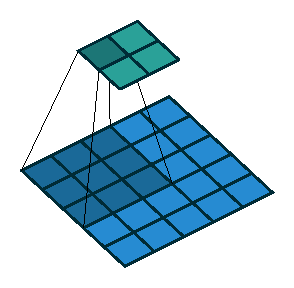
\includegraphics{graphics/no_padding_strides_00.pdf}
    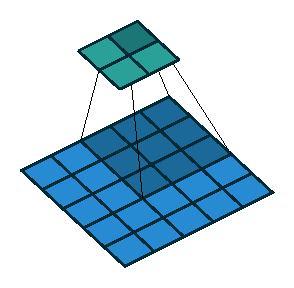
\includegraphics{graphics/no_padding_strides_01.pdf}
    \caption{Example of strided convolution without padding by \citet{dumoulin2016guide}. The left image depicts the receptive field used to compute the output element at location (1,1) in the output map. The right image depicts the receptive field used to compute the output element at location (2,1).}
    \label{fig:stridedconv}
\end{figure}

The step size by which the receptive field is moved across the input map is also called \emph{stride}. In strided convolutions, the stride is a hyperparameter that can be freely changed. This operation is defined in \Cref{eq:stridedconv}. In \Cref{eq:stridedconv}, the stride is denoted by $s \in [1,\min(W,H)]$. Note that setting the stride to $s=1$ eliminates the stride term, leading to the convolution defined in \Cref{eq:conv}. Setting the stride $s>1$ leads to a larger spacing between the receptive fields, which effectively reduces the amount of times the kernel is applied in order to produce an entry in the output matrix. Therefore, this leads to an output matrix that is smaller than the input matrix. In other words, strided convolution with $s>1$ leads to a \emph{downsampling} of the input matrix. In this aspect, it is quite similar to a pooling operation. An example of strided convolution for $s=2$ is depicted in \Cref{fig:stridedconv}.

\paragraph{Transposed Convolution}
The transposed convolution (also called deconvolution or fractionally strided convolution) operation is the inverse to strided convolution. While strided convolution downsamples the input matrix and therefore reduces the spatial dimensions, transposed convolution upsamples the input matrix in order to increase the spatial dimensions. A visual example of transposed convolution can be seen in \Cref{fig:deconvolution}. Intuitively, the input matrix is padded with empty (or, zero-valued) elements in order to produce an output matrix with increased spatial dimensions. Here, the stride hyperparameter can be interpreted as the stride of the output matrix instead of the input matrix.

\begin{figure}
\centering
    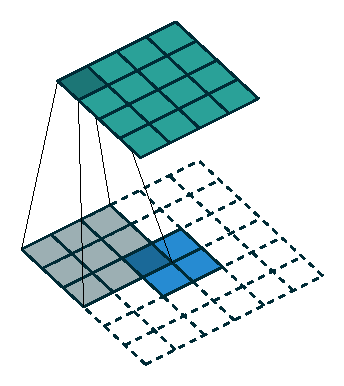
\includegraphics[width=.3\textwidth]{graphics/no_padding_no_strides_transposed_00.pdf}
    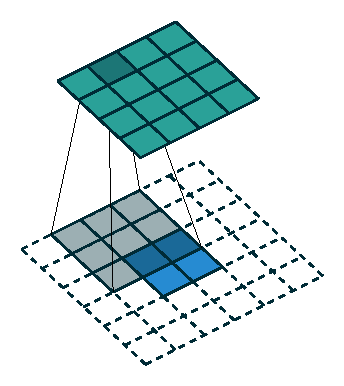
\includegraphics[width=.3\textwidth]{graphics/no_padding_no_strides_transposed_01.pdf}
    \caption{Example of a transposed convolution without padding by \citet{dumoulin2016guide}. The left image depicts the receptive field used to compute the output element at location (1,1) in the output map. The right image depicts the receptive field used to compute the output element at location (2,1).}
    \label{fig:deconvolution}
\end{figure}


\paragraph{CoordConv}
\label{subsec:bg.cnn.coordconv}
\begin{figure}
    \centering
    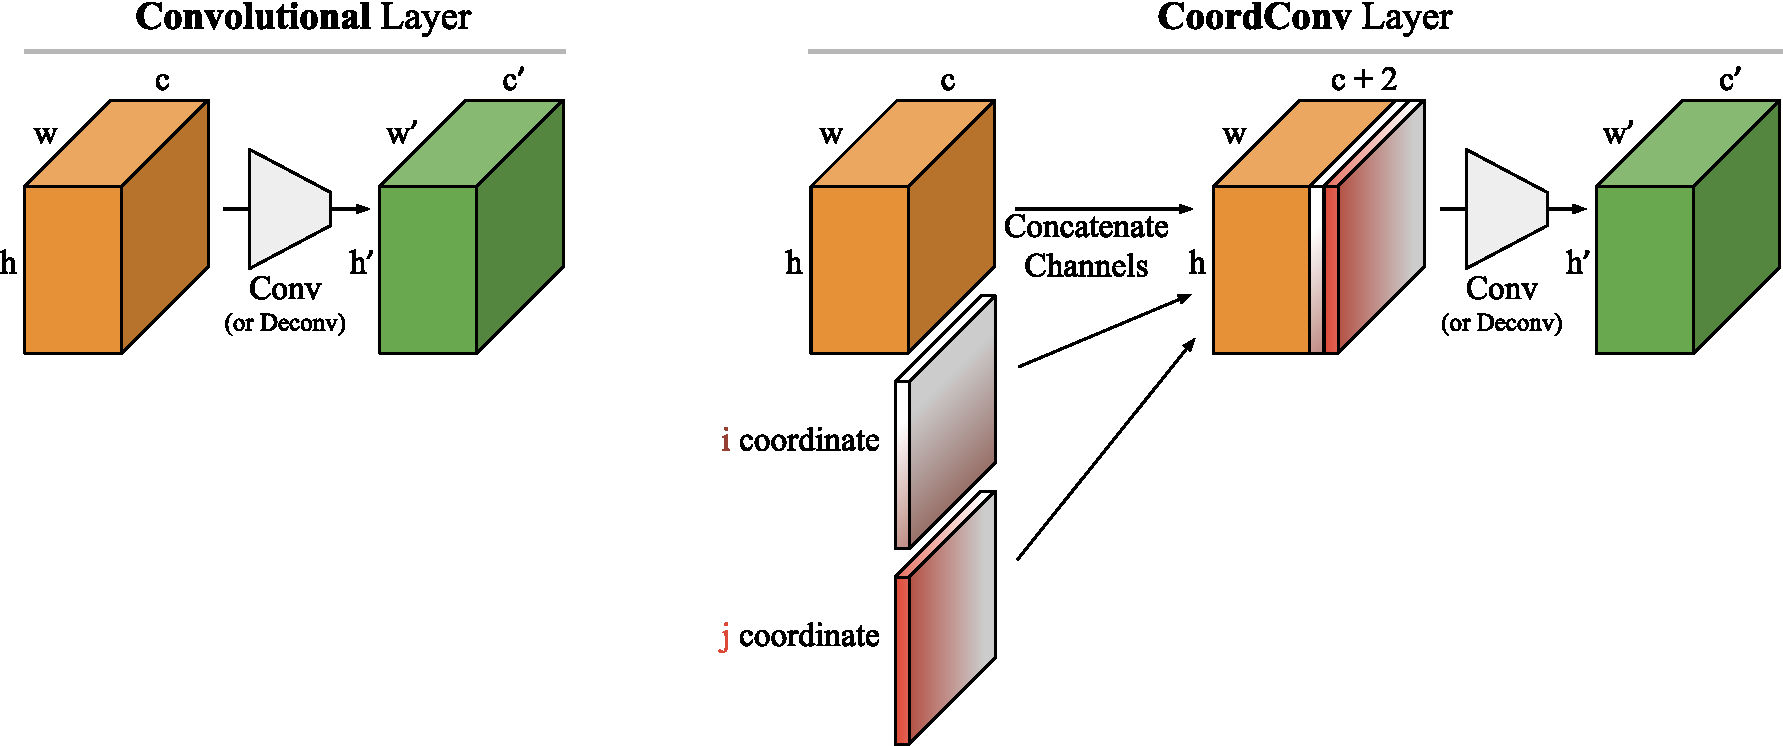
\includegraphics[width=\textwidth]{graphics/coordconv.pdf}
    \caption{Comparison of a conventional convolution layer and a CoordConv layer for input data in 2-dimensional space \citep{DBLP:conf/nips/LiuLMSFSY18}.}
    \label{fig:coordconv}
\end{figure}
An important property of convolutional layers is that they are invariant to spatial translation. However, for some tasks, this property is actually harmful. A simple example of such a task is mapping carthesian coordinates into one-hot pixel encodings, i.e., to generate an image in which the pixel at the input location is marked. In order to relax translation-invariance, \citet{DBLP:conf/nips/LiuLMSFSY18} introduced the CoordConv layer, which is depicted in \Cref{fig:coordconv}. Let $\textbf{x}\in\mathbb{R}^{W\times H\times C}$ be the input matrix to a convolutional layer. In order to preserve spatial information, explicit coordinate data is concatenated to the non-spatial dimension of the input matrix. In the usual case of 2-dimensional space, the location in space can be represented by two coordinates $(i,j)$, where $i\in [0,W)$ denotes the location in the width dimension and $j\in [0,H)$ denotes the location in the height dimension. For each spatial axis, a matrix $\mathbf{c}\in R^{W\times H}$ is concatenated to the depth dimension of $x$. In the 2-dimensional case, one coordinate matrix $\mathbf{c}_i$ is successively filled with increasing integers column-wise, while another coordinate matrix $\mathbf{c}_j$ successively filled with increasing integers row-wise. Now, by linearly combining the concatenated coordinate vectors, it is possible to uniquely identify the spatial location of each element in the original input data. In practice, the values in the coordinate vectors $c\in\mathbf{c}$ are scaled to $c\in[-1,1]$ in order to fit the scale of other input data.

Since CoordConv layers - just like convolutional layers - are fully connected in the non-spatial dimension, the explicit concatenated spatial information is used in the computation of every element in the output matrix. Since the connection weights to the coordinate vectors are freely changeable, the model is able to learn whether to use spatial information depending on the task. \citet{DBLP:conf/nips/LiuLMSFSY18} showed that CoordConv layers outperform conventional convolutional layers on a variety of tasks such as image generation, object detection and image classification.

\paragraph{1-dimensional convolution}

Motivated by a desire to apply \glspl{cnn} on sequential data such as text and inspired by \glspl{tdnn} \citep{DBLP:conf/interspeech/BottouFBL89}, \citet{DBLP:journals/jmlr/CollobertWBKKK11} introduce 1-dimensional convolutional layers, which operate on only one spatial dimension. This makes it possible to apply convolutions on sequential (or, temporal) input data, which is often arranged using using 2-dimensional matrices $\mathbf{x}\in\mathbb{R}^{t\times f}$, where $t$ is the sequence length and $f$ is the number of features per element in the sequence. By interpreting $t$ as singular spatial dimension (i.e., assuming linear space along a single axis), it is possible to define 1-dimensional (or, temporal) convolutional layers that perform the same operations as 2-dimensional convolutional layers do on input data in 2-dimensional space.

\begin{equation}
\label{eq:conv1d}
    h_{i,j}=\sum_{k=0}^c \mathbf{w}_{j,k}\mathbf{x}_{i+k}
\end{equation}
\begin{figure}
    \centering
    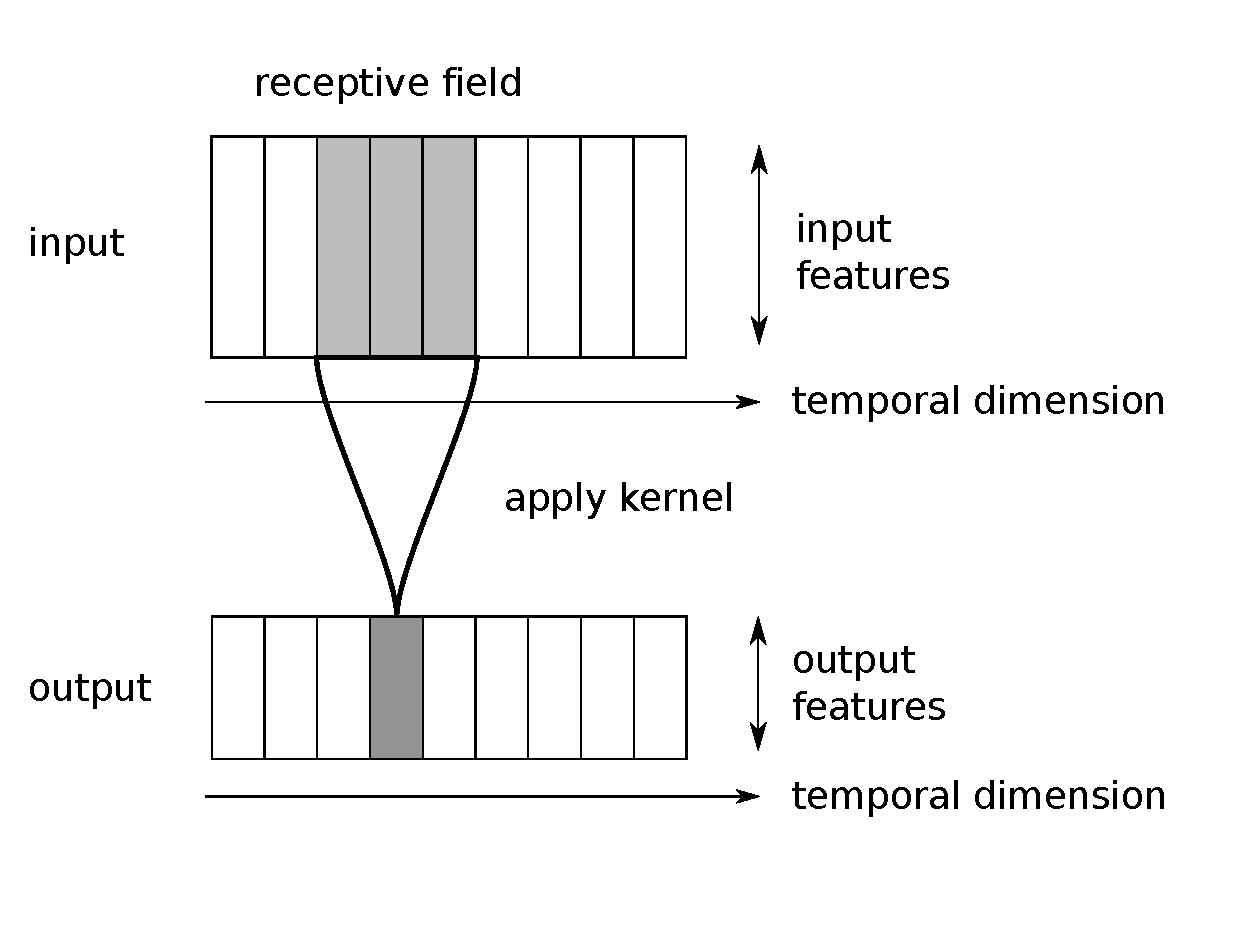
\includegraphics[width=\textwidth]{graphics/conv1d.pdf}
    \caption{Schema of a 1-dimensional convolution.}
    \label{fig:conv1d}
\end{figure}


Let $\mathbf{x}\in\mathbb{R}^{t\times f}$ be the input sequence, $c$ denote the receptive field size and $\mathbf{h}\in\mathbb{R}^{t_h\times f_h}$ be the hidden layer output, where just like in 2-dimensional convolutional layers $t_h=t$ assuming padding is used and $f_h$ is the filter size. Then, the 1-dimensional convolutional layer is defined by \Cref{eq:conv1d}, where $h_{i,j}$ is the element at location $(i,j)$ in the output matrix $\mathbf{h}$ and $\mathbf{w}\in\mathbb{R}^{f_h\times c\times f}$ is the kernel, i.e., the parameters or connection weights. The output $\mathbf{h}$ has the same dimensionality as the input sequence, with a singular spatial (or, temporal) dimension and a channel dimension the size of the numbers of filters. This way, the output of this 1-dimensional convolutional layer can in turn be used as input for a successive 1-dimensional convolutional layer, just like 2-dimensional convolutional layers. A visual example can be seen in \Cref{fig:conv1d}.

\subsubsection{Architectures}
\label{subsec:bg.cnn.arch}

While the above sections introduced the main building blocks of \glspl{cnn}, this section describes \gls{cnn} architectures that combine them in a way that has led to empirical successes \citep{ILSVRC15}.

As described in \Cref{subsec:bg.nn}, \glspl{mlp} generally perform better the deeper they are, i.e., the more hidden layers are used. This is especially true for \glspl{cnn}, which are explicitly designed to exhibit hierarchical representation learning \citep{DBLP:journals/pr/FukushimaM82,DBLP:conf/cvpr/SzegedyLJSRAEVR15}. However, it has been shown that \glspl{cnn} that exceed a certain depth threshold actually underperform \citep{DBLP:conf/cvpr/HeZRS16}. In order to solve this problem, \citet{DBLP:conf/cvpr/HeZRS16,DBLP:conf/nips/SrivastavaGS15} propose to computationally connect layer outputs that are far away in the graph. This way, the learning signal does not just propagate between directly neighbouring layers, but can \emph{skip} layers. Hence, this connection of layers at different depths is called \emph{skip connection}. Skip connections increase the diversity of paths to deeper layers, resulting in improved accuracy and faster convergence during training.

\begin{figure}
    \centering
    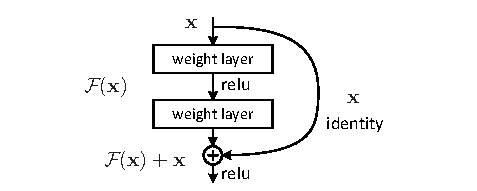
\includegraphics{graphics/residual_block.pdf}
    \caption{Residual learning block \citep{DBLP:conf/cvpr/HeZRS16}.}
    \label{fig:residual_block}
\end{figure}

A simple skip connection proposed by \citet{DBLP:conf/cvpr/HeZRS16} is the residual connection, i.e., to simply sum the outputs of a hidden layer with the outputs of a hidden layer at a different depth. This residual connection is depicted in \Cref{fig:residual_block}. This figure shows two arbitrary hidden layers in a deep \gls{cnn}, with $\mathbf{x}$ denoting the output of the preceding hidden layer, which is used as input for the first hidden layer. At the end of the block, the output of the second hidden layer is connected through addition with the identity of the output of the hidden layer preceding this block. This addition with the identity function is parameter-free and differentiable. This way, there are now two paths the signal can be propagated to, without increasing the parameter size. One path includes the intermediate first hidden layer, while the other one skips it. Note, that for the matrix addition to work both summands need to have the same dimension.

The ResNet architecture proposed by \citep{DBLP:conf/cvpr/HeZRS16} stacks a large number of residual blocks in order to form a deep \gls{cnn} which does not suffer from convergence issues. This \gls{cnn} architecture is depicted in \Cref{fig:resnet34}. The \gls{cnn} consists of an initial convolutional layer, followed by a max-pooling layer, 16 residual blocks, a gloval average-pooling layer and an ultimate fully connected layer. In total, this architecture consists of 34 layers. The input image is resized to a width and height of 224 pixels. This is a common practice for \glspl{cnn}, since high resolution input images would lead to a higher number of parameters. The first convolutional layer performs strided convolution with a stride of $s=2$, receptive field size of $c=7$ and a channel size (or, filter size) of $f=64$. Since $s=2$, the output feature map of this layer has a width and height of $224/2=112$. Afterwards, the max-pooling layer with a receptive field size of 2 further reduces this to $112/56$. This output is then used as input for the first of a sequence of 16 residual blocks. The convolutional layers in all residual blocks are performed with a receptive field size of $c=3$. Intermittently, a strided convolution with $s=2$ is used in order to halve the output size. The convolutional layer immediately following such a halving has double the filter size of the preceding layer $f_{i+1}=f_i*2$. All other convolutional layers have the same filter size as their predecessor.

\begin{figure}
\centering
    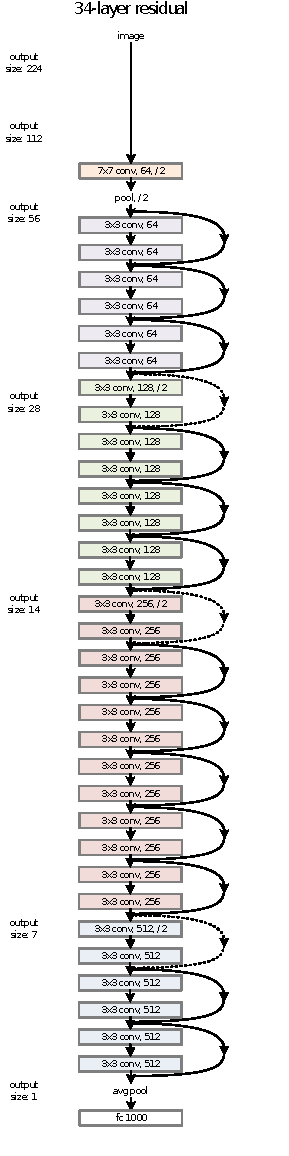
\includegraphics{graphics/arch.pdf}
    \caption{ResNet architecture design with 34 layers and residual blocks instead of bottleneck blocks \citep{DBLP:conf/cvpr/HeZRS16}.}
    \label{fig:resnet34}
\end{figure}

%\begin{wrapfigure}{l}{.4\textwidth}
%    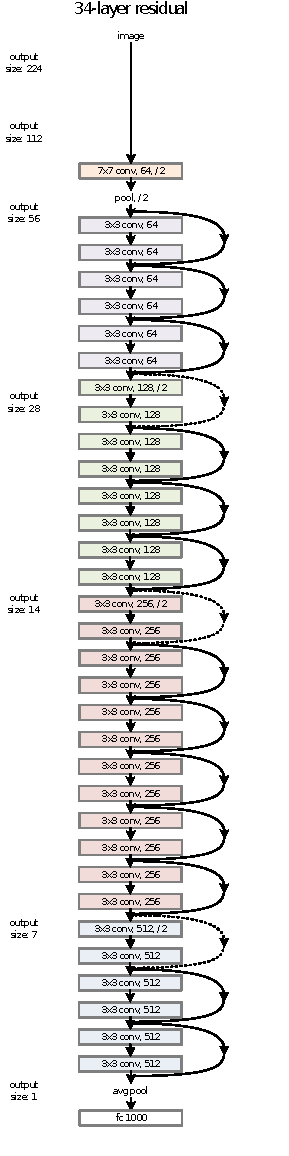
\includegraphics{graphics/arch.pdf}
%    \caption{ResNet architecture design with 34 layers and residual blocks instead of bottleneck blocks \citep{DBLP:conf/cvpr5/HeZRS16}.}
%    \label{fig:resnet34}
%\end{wrapfigure}

Recall that for addition in the residual connection, the summands need to have the same dimension. This means, given that layers $i$ and its successor $j$ have a different filter size than preceding layer $h$, a residual connection of $h$ to $j$ is not possible. In order to enable such a connection, a convolutional layer with receptive field size $c=1$ is applied on the output of the preceding layer $\textbf{o}_h$ before being added to the output of the connected layer $\textbf{o}_j$. Crucially, the filter size of this 1x1-convolution is identical to the the filter size of the succeeding layers $i$ and $j$. Since $c=1$, the convolution preserves the spatial dimensions of the output, but changes the filter size to match layers $i$ and $j$. This \emph{projection shortcut} enables residual connections across layers with different filter sizes, but also introduces (a low amount of) additional parameters. It is preferable to keep filter sizes constant in order to use parameter-free residual connections as much as possible. In the few instances in which the filter size changes in the ResNet architecture, projection shortcuts have to be used immediately afterwards. These are indicated by dotted arrows in \Cref{fig:resnet34}.

%Note that the output feature map at the end of the convolutional layers is 3-dimensional. This output structure is not suited for the most tasks \gls{cnn} are used for, which require 1-dimensional vectors. Taking the example of image classification, which requires as output a one-dimensional vector consisting of as many entries as there are classes.

Since the ResNet architecture was trained and tested for an image classification task, the output feature map has to be structured into a vector with a cardinality of 1000 (which is the number of classes in the ImageNet dataset \citep{ILSVRC15}). In order to achieve this, global average-pooling is used in order to reduce the output feature matrix into a vector with cardinality 512, which is the filter size of the ultimate convolutional layer. Afterwards, a fully connected layer is used to produce an output vector of cardinality 1000.

\begin{figure}
    \centering
    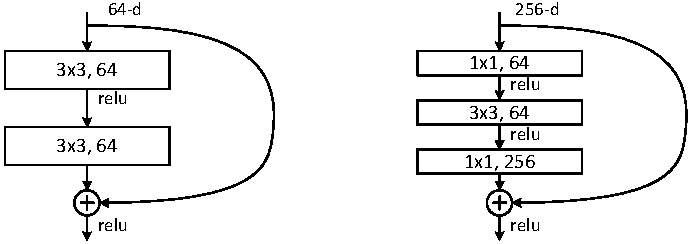
\includegraphics{graphics/block_deeper.pdf}
    \caption{Comparison of a residual block (left) and a bottleneck block (right) \citep{DBLP:conf/cvpr/HeZRS16}.}
    \label{fig:bottleneck}
\end{figure}

The 34-layer ResNet described above was empirically shown to solve the degradation problems experienced by deep \gls{cnn} without residual connections \citep{DBLP:conf/cvpr/HeZRS16}. Therefore, \citet{DBLP:conf/cvpr/HeZRS16} introduced ResNet architectures that were even deeper. For computational efficiency, residual blocks are replaced by \emph{bottleneck} blocks, which are depicted in \Cref{fig:bottleneck}. Here, the two convolutional layers of residual blocks are replaced with three convolutional layers. The first convolutional layer has a receptive field size $c=1$ and a filter size $f=64$. This layer solely serves to reduce the filter size. The succeeding convolutional layer with a receptive field size of 3 performs the usual feature extraction on this reduced filter size. The final convolutional layer again has a receptive field size of 1 and a filter size of 256. As an inverse to the first layer, it serves to increase the filter size to the same size it is in output of the preceding block. This way, the convolutional layer performing feature extraction is a bottleneck with smaller input and output filter size. This serves both as regularization and to increase computational efficiency.

By replacing all residual blocks in the ResNet-34 architecture with bottleneck blocks, the number of layers is increased to 50. \citet{DBLP:conf/cvpr/HeZRS16} show that this model already performs better than ResNet-34. \citet{DBLP:conf/cvpr/HeZRS16} build even deeper models by stacking more bottleneck blocks, arriving at a ResNet model with 152 layers, which yielded the best empirical results.

The ResNet architecture has been widely used to create deep \gls{cnn} architectures. There exists a range of extensions and modifications to the original architecture, including ResNetv2 \citep{DBLP:conf/eccv/HeZRS16}, Wide ResNet \citep{DBLP:conf/bmvc/ZagoruykoK16}, ResNeXt \citep{DBLP:conf/cvpr/XieGDTH17} and most recently ConvNeXt \citep{DBLP:conf/cvpr/0003MWFDX22}.


\subsection{Recurrent Neural Networks}
\label{subsec:bg.rnn}

While the \gls{mlp} is a general purpose architecture and the \gls{cnn} has an inductive bias for spatial data, the recurrent neural network is a neural network architecture with an inductive bias for sequential (or, temporal) data. The original architecture introduced by \citet{Rumelhart1986} equips neural networks with memory capabilities. In contrast to other neural network architectures such as \glspl{mlp} or \glspl{cnn}, individual forward passes on inputs are not independent. Let $\mathbf{x}_n$ be an input sequence. Just like with neural networks, recurrent neural networks perform a forward pass according to $f(\mathbf{x}_0; \boldsymbol{\theta})$. Contrary to neural networks, the forward pass for the next input $\mathbf{x}_1$ depends on the forward pass of the previous input, i.e., $f(\mathbf{x}_1;\boldsymbol{\theta};f(\mathbf{x}_0; \boldsymbol{\theta}))$. This loop-like functionality enables \glspl{rnn} to take previous inputs and predictions into account when computing new predictions. The simple \gls{rnn} architecture is defined in \Cref{eq:vanillarnn.h,eq:vanillarnn.o}.

\begin{equation}
\label{eq:vanillarnn.h}
        \mathbf{h_t} = \phi(\mathbf{h}_{t-1} \boldsymbol{\theta}_h + \mathbf{x}_t \boldsymbol{\theta}_x)
\end{equation}

\begin{equation}
\label{eq:vanillarnn.o}
        \mathbf{o}_t = \mathbf{h_t} \boldsymbol{\theta}_o
\end{equation}

Note that all variables in \Cref{eq:vanillarnn.h,eq:vanillarnn.o} are temporal, i.e., depend on $t$. Only the learnable parameters $\boldsymbol{\theta}$ are constant. $\mathbf{h}_t$ is the state of recurrent neural network. It represents all individual inputs and state changes up to  $\mathbf{x}_t$. The output $\mathbf{o}_t$ is computed by taking the current state $\mathbf{h}_t$ into account. Thus, a \gls{rnn} can natively handle temporal inputs.

Recurrent neural networks are optimized in the same way as standard neural networks. However, due to the temporal component introduced in \Cref{eq:vanillarnn.h,eq:vanillarnn.o}, the gradient can not be computed using standard backpropagation. The gradients needed for loss function optimization are computed using the backpropagation-through-time algorithm \citep{robinson:utility}.

In practice, standard recurrent neural networks are not able to generalize well and do not take long-term dependencies into account because they suffer from vanishing or exploding gradients \citep{hochreiterdipl,Bengio:1994:LLD:2325857.2328340}.

\subsubsection{Gated Recurrent Units}

In order to alleviate the convergence problems of standard recurrent neural networks, \citet{Hochreiter:1997:LSM:1246443.1246450} introduced the \gls{lstm} recurrent neural network. In addition to the hidden state $\mathbf{h}_t$, it introduces a cell state $\mathbf{c}$ and a corresponding set of update equations which do not suffer from gradient problems. A simplified variant of the \gls{lstm} architecture are \glspl{gru} \citep{cho14}. Its authors claim that \glspl{gru} work better than \glspl{lstm}. \Crefrange{eq:gru1}{eq:gru4} detail the update procedure similar to \Cref{eq:vanillarnn.h,eq:vanillarnn.o}. Note that $\mathbf{o}_t = \mathbf{h}_t$.

\begin{equation}
\label{eq:gru1}
        \mathbf{z}_t = \phi_\text{sigmoid}([\mathbf{h}_{t-1},\mathbf{x}]\boldsymbol{\theta}_z)
\end{equation}

\begin{equation}
\mathbf{r}_t = \phi_\text{sigmoid}([\mathbf{h}_{t-1},\mathbf{x}]\boldsymbol{\theta}_r)
\end{equation}

\begin{equation}
\mathbf{\tilde{h}}_t = \phi_\text{tanh}([\mathbf{r}_t \mathbf{h}_{t-1},\mathbf{x}]\boldsymbol{\theta}_h)
\end{equation}

\begin{equation}
\label{eq:gru4}
\mathbf{h}_t = (1 - \mathbf{z}_t) \mathbf{h}_{t-1} + \mathbf{z}_t \mathbf{\tilde{h}}_t
\end{equation}

It is still unknown whether \glspl{gru} truly improve upon \glspl{lstm}. A large-scale study \citep{7508408} compared \gls{lstm} variants on speech recognition, handwriting recognition and music modeling tasks and found no significant difference. Another study \citep{pmlr-v37-jozefowicz15} used a different hyperparameter optimization algorithm and compared \glspl{lstm} and \glspl{gru} on arithmetic, XML modeling, language modeling and music modeling tasks. They conclude that \glspl{gru} perform better than \glspl{lstm}.

\subsubsection{CNN or RNN?}

As discussed in \Cref{subsec:bg.cnn} and \Cref{subsec:bg.rnn}, both 1-d convolutional and recurrent neural networks can handle temporal data. While only \glspl{rnn} can properly handle sequences of unknown length, for input data of fixed length, it is of interest to know which architecture is better suited. This comparison was investigated by \citet{2017arXiv170201923Y,2018arXiv180301271B}. Both come to the conclusion that 1-dimensional \glspl{cnn} lead to better and faster convergence than \glspl{rnn} on sequence classification tasks. Keep in mind, however, that the empirical results using toy problems might not generalize.


\subsection{Transformer}
\label{subsec:bg.tf}

The Transformer introduced by \citet{DBLP:conf/nips/VaswaniSPUJGKP17} is a neural network architecture that essentially combines the advantages of \glspl{rnn} and \glspl{cnn}. Like \glspl{rnn}, it can be used for sequential data, but like \glspl{cnn} it can be efficiently computed on \glspl{gpu} using matrix multiplications. The Transformer consists almost solely of \emph{self-attention} modules, which are explained below.

\subsubsection{Self-Attention}
Attention is a general purpose mechanism for neural networks introduced by \citet{DBLP:journals/corr/BahdanauCB14} and was originally intended for machine translation \glspl{rnn}. It allows to assign each element $\mathbf{x}_i$ of an input set $\mathbf{X}$ an attention weight $\alpha_i$. Crucially, this mechanism is differentiable, so it can be fitted along with the neural network model.

Originally, attention was intended to compute values using both an input sequence (text in \citet{DBLP:journals/corr/BahdanauCB14}) and an output sequence (\gls{rnn} hidden states in \citet{DBLP:journals/corr/BahdanauCB14}). However, the form of attention used for Transformers operates over a single input sequence only. This form is called \emph{self-attention} (or inter-attention).

Let $\mathbf{X} \in \mathbb{R}^{n\times m}$ be a set of $n$ elements with $m$ features. In the general form, the self-attention mechanism transforms $\mathbf{X}$ into a \emph{contextualized} set $\mathbf{Y} \in \mathbb{R}^{n \times m}$. The resulting set is of the same length as $\mathbf{X}$ and $\mathbf{y}_i \in \mathbf{Y}$ can be interpreted as representing the value of $\mathbf{x}_i \in \mathbf{X}$ taking into consideration all other elements of $\mathbf{X}$. Mathematically, this can be achieved by first computing \emph{attention weights} $\mathbf{A}$ as the dot-product of $\mathbf{X}$ with itself, as can be seen in \Cref{eq:attn}. This equation uses the unit softmax function defined in \Cref{eq:softmax} to produce a pseudo-probability distribution from the unbounded attention scores, i.e., to bound them to $[0,1]$ and let them sum to 1. The contextualized set $\mathbf{Y}$ can then be computed as the weighted sum of $\mathbf{X}$ using the attention weights, as defined in \Cref{eq:attn.res}.

\begin{equation}
        \label{eq:attn}
        \mathbf{A} = \text{softmax}(\mathbf{X}\mathbf{X}')
\end{equation}

\begin{equation}
        \label{eq:softmax}
        \text{softmax}(\mathbf{x})_i=\frac {\exp(x_i)}{\sum_{j=1} ^{|\mathbf{x}|} \exp(x_j)}
\end{equation}

\begin{equation}
        \label{eq:attn.res}
        \mathbf{y}_i = \sum_{j=1}^{n} \alpha_{ij} \mathbf{x}_j
\end{equation}

In conclusion, the element $\mathbf{y}_i \in \mathbf{Y}$ is computed by \emph{attending} to individual elements of $\mathbf{X}$ with different weights. This attention variant using a weighted sum introduced here is also called \emph{soft attention}, since all input elements contribute to the output. There also exists hard attention described in \citet{pmlr-v37-xuc15}, which explicitly selects elements instead of using a weighted sum of all elements. Since this is not differentiable, it is more complex to integrate it in the optimization procedure.

This self-attention mechanism can be further extended with learnable parameters. Notice in \Cref{eq:attn,eq:attn.res} that $\mathbf{X}$ is used three times in the self-attention mechanism. Different learnable parameters $\mathbf{W}\in\mathbb{R}^{m\times m}$ are used for these three occurrences.  To distinguish them more easily, these are defined analogous to a continuous dictionary as query $\mathbf{Q}=\mathbf{X}\mathbf{W_Q}$, key $\mathbf{K}=\mathbf{X}\mathbf{W_K}$ and value $\mathbf{V}=\mathbf{X}\mathbf{W_V}$. In \Cref{eq:attn.kqv}, the query and the key are matched to produce a compatibility (i.e., the attention weights), which is then used in \Cref{eq:attn.res.kqv} to retrieve the values. It is also clear that this attention variant is called \emph{self-attention} because $\mathbf{Q}$, $\mathbf{K}$ and $\mathbf{V}$ are computed using the same input $\mathbf{X}$.

\begin{equation}
        \label{eq:attn.kqv}
        \mathbf{A} = \text{softmax}(\mathbf{Q}\mathbf{K}')
\end{equation}

\begin{equation}
        \label{eq:attn.res.kqv}
        \mathbf{Y} = \mathbf{A} \mathbf{V}
\end{equation}

The self-attention variant described until now is called \emph{dot-product attention} \citep{DBLP:conf/emnlp/LuongPM15,DBLP:journals/corr/GravesWD14}. There also exists \emph{additive attention} \citep{DBLP:journals/corr/BahdanauCB14}. This approach first computes attention scores $s_{ij}$ by concatenating $\mathbf{q_i}$ and $\mathbf{k'_j}$ and using the concatenated vector as an input to a single layer \gls{mlp}. This can be seen in \autoref{eq:attn.add}. In this equation, $\mathbf{q}_i \| \mathbf{k}_j\in \mathbb{R}^{nm}$, $\mathbf{W_A}\in \mathbb{R}^{nm}$ are the learnable parameters and $\phi$ is a non-linearity such as the tanh function. Then in \Cref{eq:attn.add.soft} the softmax function is used to compute the attention weights.

\begin{equation}
        \label{eq:attn.add}
        s_{ij} = \phi(\mathbf{W_A}[\mathbf{q}_i \| \mathbf{k}_j])
\end{equation}

\begin{equation}
        \label{eq:attn.add.soft}
        \alpha_{ij}=\text{softmax}(\mathbf{s})_{ij}
\end{equation}

In practice, additive attention leads to better results than dot-product attention if the feature dimension $m$ is large \citep{britz-etal-2017-massive}. However, it can be seen that, to compute the entire attention matrix $\mathbf{A}$, additive
attention needs to use the neural network $nm$ times. This cannot be restructured into a single matrix multiplication due to the non-linearity. Contrary to that, dot-product attention can simply be computed using a matrix multiplication, which is more suited for GPU workloads. To remedy this situation, \emph{scaled} dot-product attention \citep{DBLP:conf/nips/VaswaniSPUJGKP17} has been introduced. This simply normalizes the dot product by $1/\sqrt{m}$ to counteract the adverse effect of large values of $m$ and has largely replaced additive attention.

\begin{equation}
        \label{eq:attn.scal.kqv}
        \mathbf{A} = \text{softmax}\left(\frac{\mathbf{Q}\mathbf{K}'}{\sqrt{m}}\right)
\end{equation}

Another way of stabilizing self-attention is multi-head attention \citep{DBLP:conf/nips/VaswaniSPUJGKP17}, which is analogous to using multiple channels in \glspl{cnn}. Multiple heads of the self-attention function $h$ are computed in parallel using different learnable parameters in \autoref{eq:attn.multi}. The $h$ output matrices are concatenated and projected to the original dimension $\mathbb{R}^{n\times m}$ using the learnable linear transformation $\mathbf{W}_\mathbf{Y}\in\mathbb{R}^{n \times nh}$ in \autoref{eq:attn.multi.res}. Intuitively, this allows to attend to different embeddings simultaneously. \citet{DBLP:conf/nips/VaswaniSPUJGKP17} set $h=8$ for their architecture.

\begin{equation}
        \label{eq:attn.multi}
        \mathbf{Y}^{\text{head}_i}=\text{Self-Attention}(\mathbf{X}; \mathbf{W}^i_\mathbf{Q}, \mathbf{W}^i_\mathbf{K}, \mathbf{W}^i_\mathbf{V}).
\end{equation}

\begin{equation}
        \label{eq:attn.multi.res}
        \mathbf{Y}= \mathbf{W}_\mathbf{Y}  \left(\|_{i=0}^{h} \mathbf{Y}^{\text{head}_i}\right) 
\end{equation}


The main computational problem of standard self-attention is that its space and time complexity is quadratic in the set length $n$. This quickly becomes a problem for larger values of $n$. Multiple approaches were proposed to modify self-attention to achieve lower runtime, memory or IO complexity \citep{DBLP:conf/iclr/ChoromanskiLDSG21,DBLP:conf/nips/DaoFERR22}.

Another approach to solve this computational problem is local attention \citep{DBLP:conf/emnlp/LuongPM15}. The self-attention variant described above can be seen as \emph{global} attention, since it uses the entire input set $\mathbf{X}$ to compute each output vector $\mathbf{y}_i$. In local attention, only a constant number of neighbours is used. This is computationally more efficient, but restricts the contextualized output vectors from taking longer-range dependencies into account. In practice, most works utilize standard self-attention and deal with the complexity by increasing hardware resources.

\subsubsection{Standard Transformer}

\begin{figure}[h]
        \centering
        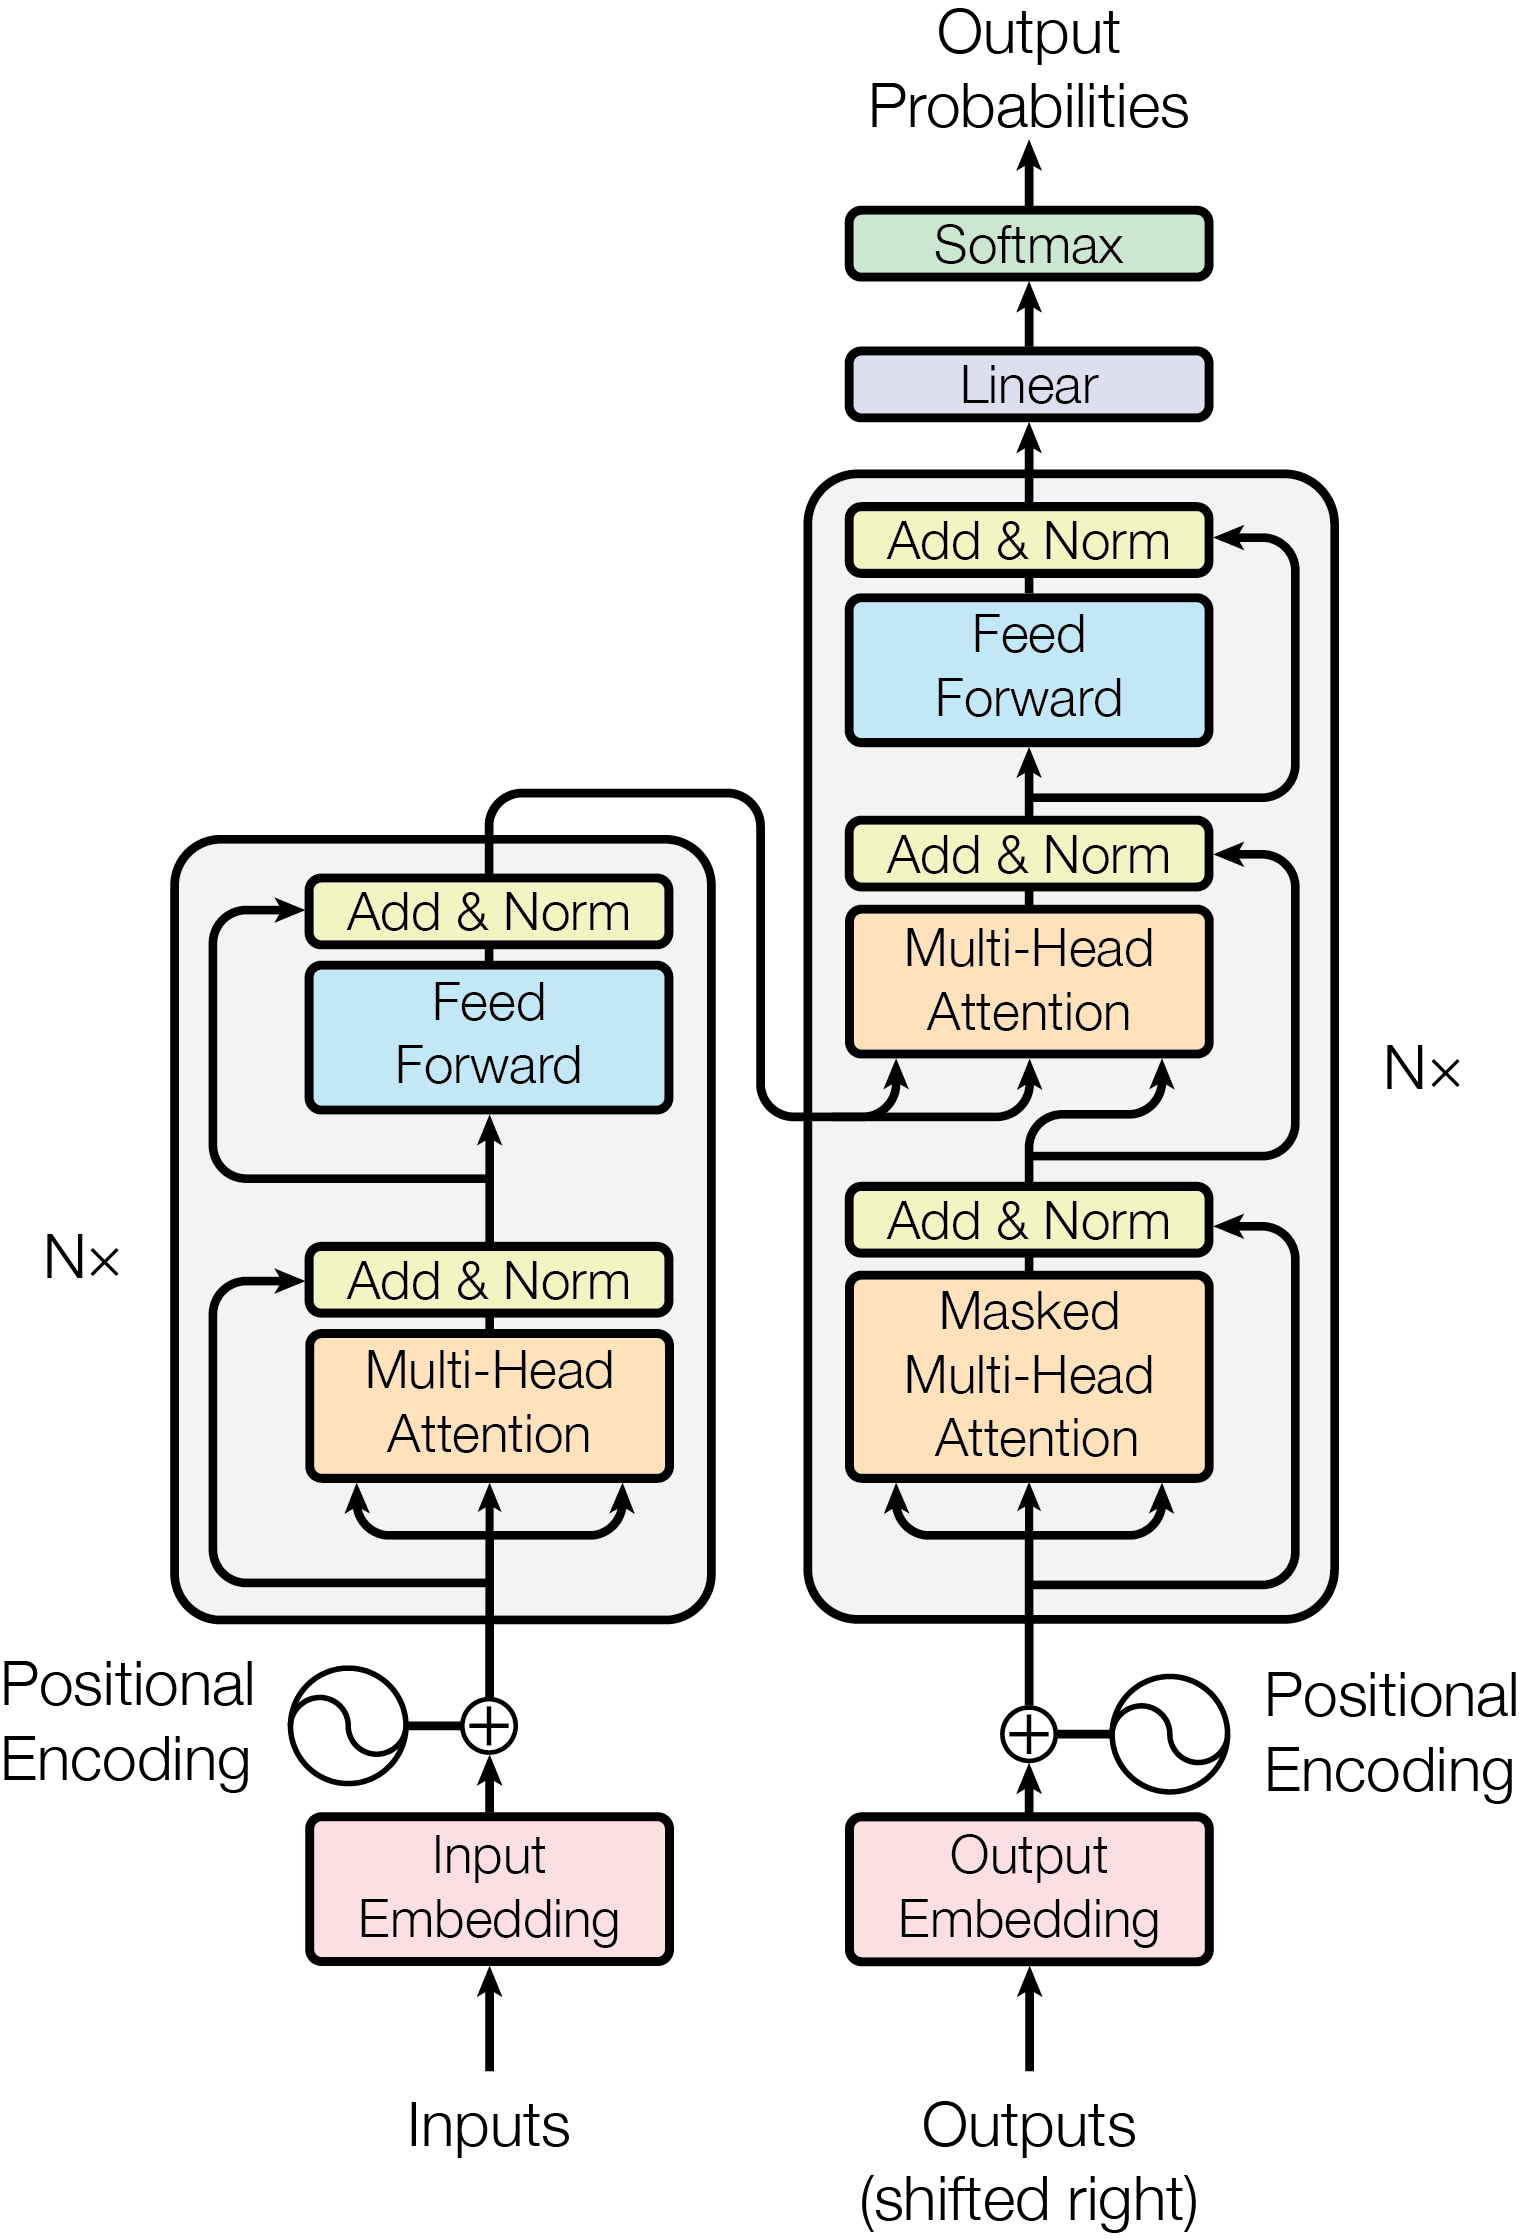
\includegraphics[width=.3\textwidth]{graphics/ModalNet-21}
        \caption{Transformer architecture by \citet{DBLP:conf/nips/VaswaniSPUJGKP17}.}
        \label{fig:transformer}
\end{figure}

While (self-)attention was originally only used as an add-on for \glspl{rnn}, the Transformer architecture introduced by \citet{DBLP:conf/nips/VaswaniSPUJGKP17} consists solely of global scaled self-attention modules stacked with an \gls{mlp}. They showed that this is not only simpler but actually preferable to using \glspl{rnn}. While the Transformer uses a fixed number of self-attention modules, an \gls{rnn} requires $n$ sequential operations. This is an advantage, since it has been established that a shorter path length between two positions makes it easier to learn long-range dependencies \citep{5264952}.

The Transformer architecture is depicted in \Cref{fig:transformer} and consists of stacked transformer blocks, with each block consisting of multi-head self-attention and layer normalization \citep{DBLP:journals/corr/BaKH16} (similar to batch normalization as described in \Cref{subsec:bg.nn.batchnorm}) followed by a simple \gls{mlp} and layer normalization. The \gls{mlp} is position-wise, i.e., it is applied to each output vector $\mathbf{y}_i$ individually. The architecture employs residual connections \citep{7780459} around each individual block step.

The Transformer architecture can be used for any kind of real-valued set data. Originally, it was intended for \gls{nlp} tasks and thus to beused with text data as input. However, text data is sequential in nature, while the Transformer architecture does not preserve order information due to the permutation-equivariant self-attention layers. This is similar to using 1-dimensional CoordConv layers as described in \Cref{subsec:bg.cnn.coordconv}. In order to be able to use sequential data, the Transformer architecture concatenates a positional encoding to each input element before applying self attention. The Transformer architecture employs global attention and thus computes the attention of all input pairs.

Since the Transformer continually leads to new successes in \gls{nlp} \citep{DBLP:conf/naacl/DevlinCLT19,DBLP:conf/nips/BrownMRSKDNSSAA20,DBLP:journals/corr/abs-2302-13971}, there have been numerous attempts to apply it on visual data. These \glspl{vit} perform comparably and in some cases outperform \glspl{cnn} on a variety of tasks such as image classification and object detection \citep{DBLP:conf/iclr/DosovitskiyB0WZ21,liu2021Swin}.


\subsection{Encoder-Decoder Framework}
\label{subsec:bg.vae}

An important general framework for generative deep learning architectures is the encoder-decoder framework. To motivate this, first, the \emph{autoencoder} architecture \citep{https://doi.org/10.1002/aic.690370209} is introduced.

Recall that neural networks are universal function approximators, i.e., they approximate an arbitrary real-valued ground truth function $F(\textbf{x})=\textbf{y}, F: \mathcal{X} \rightarrow \mathcal{Y}$ using freely changeable parameters $\boldsymbol{\theta}$ as $f(\mathbf{x};\boldsymbol{\theta})$. In many tasks, the input and output data are part of different vector spaces, e.g. in image classification $\mathbf{x}\in\mathcal{X}$ being an image and $\mathbf{y}\in\mathcal{Y}$ being the class probabilities. The autoencoder architecture was introduced by \citet{https://doi.org/10.1002/aic.690370209} to solve the task of condensing the input $\mathbf{x}$ into a an efficient (i.e., smaller) code $\mathbf{z}\in\mathcal{Z}$, which can be used to fully reconstruct $\mathbf{x}$. It must hold, then, that this code contains all essential information about the input data. This code is referred to as \emph{latent code}, or, since it is represented as a vector, \emph{latent vector}.

\begin{figure}
    \centering
    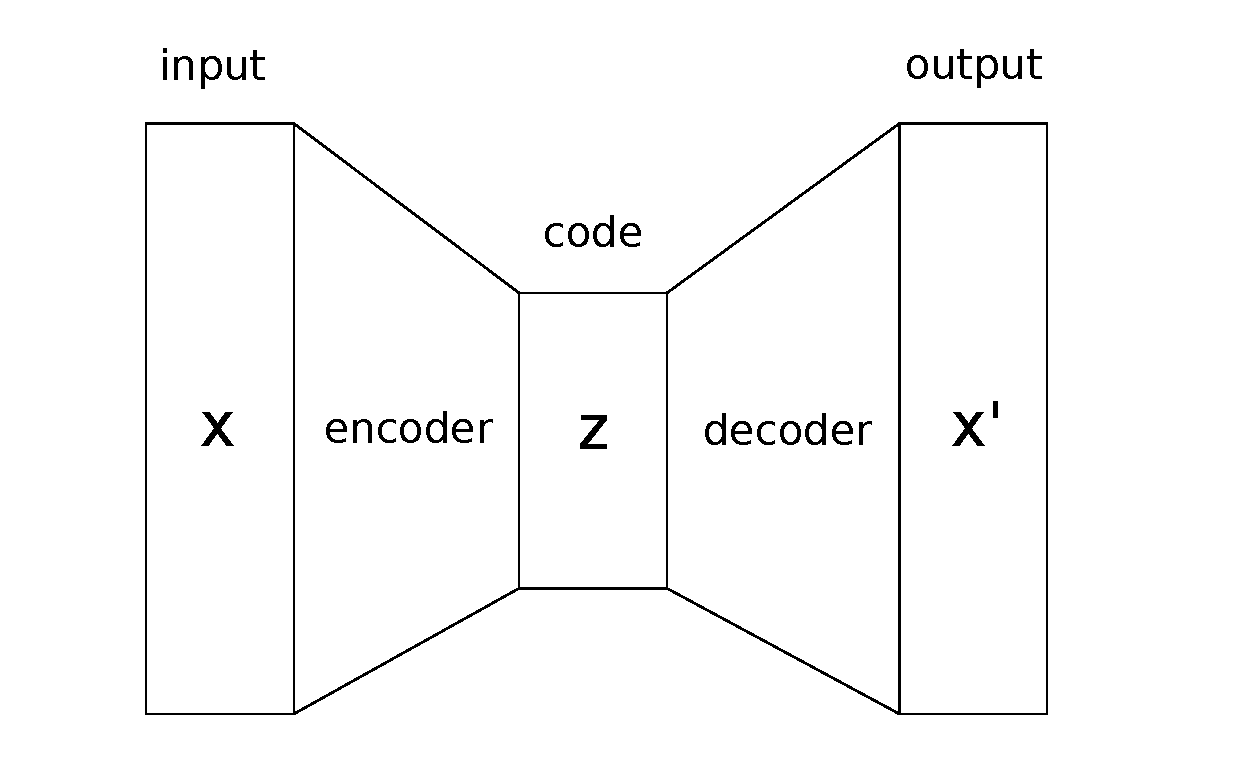
\includegraphics[width=\textwidth]{graphics/autoencoder.pdf}
    \caption{Schema of the autoencoder architecture.}
    \label{fig:autoencoder}
\end{figure}

For the purpose of finding efficient encodings, the autoencoder consists of two neural networks. The \emph{encoder} $e$ defined in \Cref{eq:autoencoder.enc} is an \gls{mlp} which maps the input $\mathbf{x}\in\mathcal{X}$ to the latent vector $\mathbf{z}\in\mathcal{Z}$ using freely changeable parameters $\boldsymbol{\theta}_e$. In turn, the \emph{decoder} $d$ defined in \Cref{eq:autoencoder.dec} is an \gls{mlp} which maps the latent vector $\mathbf{z}$ to an output vector $\mathbf{x'}\in\mathcal{X}$ with $\mathbf{x'}\approx\mathbf{x}$ (or, in the optimal case $\mathbf{x'}=\mathbf{x}$) using freely changeable parameters $\boldsymbol{\theta}_d$. The complete autoencoder is then defined by \Cref{eq:autoencoder} and depicted in \Cref{fig:autoencoder}. The autoencoder is optimized using gradient descent of a loss function measuring the distance between $\mathbf{x}'$ and $\mathbf{x}$ such as the $L^1$ or $L^2$ distance described in \Cref{subsec:bg.losses}. Furthermore, an important design consideration is that the latent vector is smaller than the input vector, since if $\dim(\mathbf{z})=\dim(\mathbf{x})$, the autoencoder might converge to the identity function as local optimum.


\begin{equation}
\label{eq:autoencoder.enc}
    \mathbf{z}=e(\mathbf{x};\boldsymbol{\theta}_e)
\end{equation}\begin{equation}
\label{eq:autoencoder.dec}
    \mathbf{x'}=d(\mathbf{z};\boldsymbol{\theta}_d)
\end{equation}
\begin{equation}
\label{eq:autoencoder}
    \mathbf{x'}=d(\mathbf{z};\boldsymbol{\theta}_d)=d(e(\mathbf{x};\boldsymbol{\theta}_e);\boldsymbol{\theta}_d)
\end{equation}

Autoencoders were proposed for dimensionality reduction, since the latent vector theoretically contains all necessary information of the input data in smaller form. This can be useful as a compression technique. Additionally, it is possible to apply vector space operations on the latent vector that might not have been possible or practical on the input data, such as linear transformations or distance measures. Furthermore, it is possible to use autoencoders for generative tasks by using the decoder of an optimized autoencoder on its own. By sampling an arbitrary $\mathbf{z}_k\in\mathcal{Z}$ and inputting it into an optimized $d$, it is possible to generate new output data $\mathbf{x}'_k\in\mathcal{X}$ that follows the same distribution of the training input data (e.g. if $\mathcal{X}$ is an image space, generating new images that are similar to the images in the training dataset). In turn, since the encoder is differentiable, optimized encoders can also be used on their own for downstream tasks. For this reason, autoencoders have found a wide range of applications \citep{DBLP:conf/ssst/ChoMBB14,DBLP:conf/iclr/TheisSCH17,doi:10.1126/science.1127647}.

By generalizing the autoencoder to inputs and outputs of different distributions, one arrives at the encoder-decoder framework \citep{DBLP:conf/nips/SutskeverVL14,FITPT283} as depicted in \Cref{fig:encoderdecoder}, which is used by a wide variety of recently successful neural network architectures such as the Transformer (as explained in \Cref{subsec:bg.tf}). As an example, \citet{DBLP:journals/corr/abs-1301-3781} use an encoder-decoder architecture to encode words (i.e., character sequences) into semantically meaningful latent vectors. The encoder-decoder framework is defined in \Cref{eq:encdec}, which is a generalization of \Cref{eq:autoencoder}. Note that the output vector $\mathbf{y}\in\mathcal{Y}$ of the decoder $d$ follows a different distribution than the input vector $\mathbf{x}\in\mathcal{X}$. Furthermore, the optimization objective is not $\mathbf{y}=\mathbf{x}$, as is the case in autoencoders, but is replaced with a task-dependent objective.

\begin{figure}
    \centering
    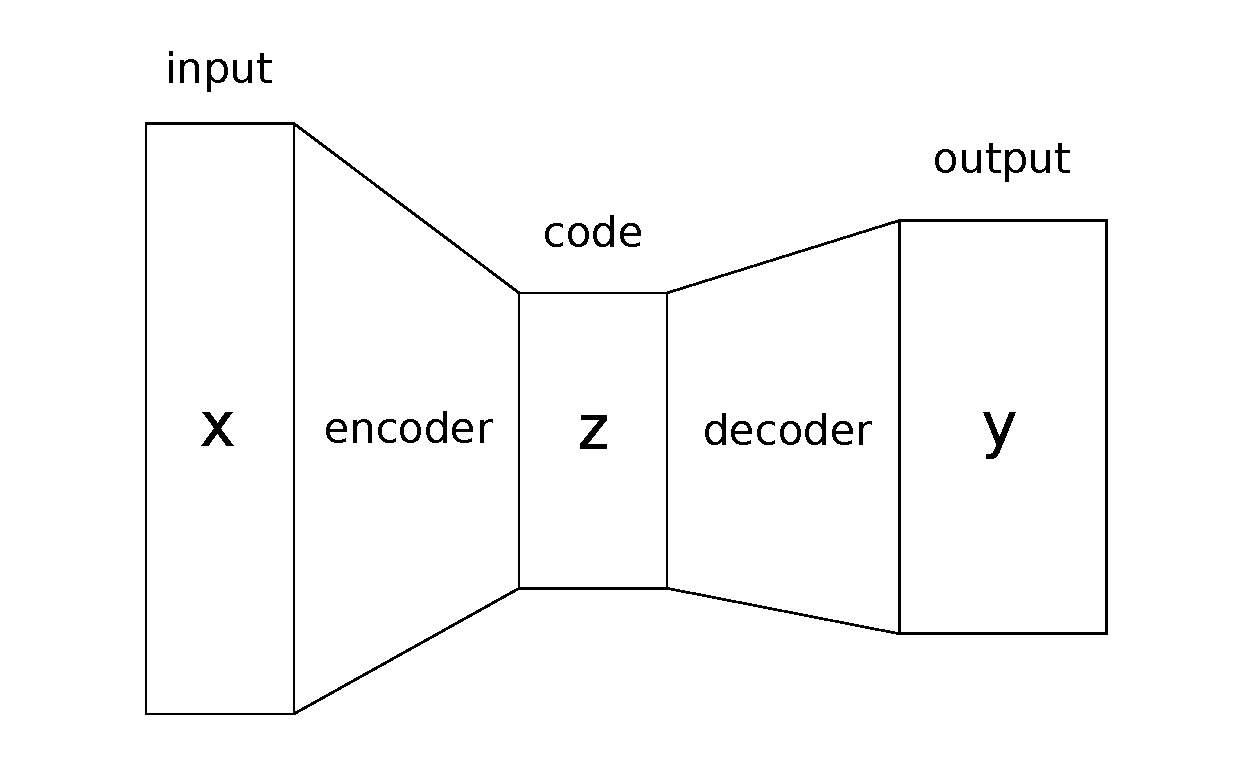
\includegraphics[width=\textwidth]{graphics/encoderdecoder.pdf}
    \caption{Schema of an architecture following the encoder-decoder framework.}
    \label{fig:encoderdecoder}
\end{figure}

\begin{equation}
\label{eq:encdec}
    \mathbf{y}=d(\mathbf{z};\boldsymbol{\theta}_d)=d(e(\mathbf{x};\boldsymbol{\theta}_e);\boldsymbol{\theta}_e)
\end{equation}


As an aside, there exist different versions of and modifications to the autoencoder architecture. Chief among them is the \gls{vae}, which attempts to normalize the latent space $\mathcal{Z}$ s.t. $\forall z_i\in\mathbf{z}\in\mathcal{Z}$, $z_i \sim \mathcal{N}(0,1)$, where $N(\mu,\sigma)$ is a normal distribution with mean $\mu$ and standard deviation $\sigma$. In order to achieve this, a loss term which calculates the  divergence between $\mathbf{z}$ and the standard-normal distribution $\mathcal{N}(0,1)$ is added to the autoencoder loss. Usually, \gls{kl} divergence \citep{10.1214/aoms/1177729694} is chosen as loss function.

\subsubsection{Feature Combination}
There exist encoder-decoder architectures with multiple encoders but only one decoder, most commonly if input from different modalities is used to generate a single output. In this case, multiple latent vectors have to be combined into a single latent vector suitable for consumption by the decoder. This is referred to as \emph{feature combination}, or \emph{feature fusion}. Two common types of feature combination are introduced in this section.

\begin{equation}
    \label{eq:concatfeaturefusion}
    \mathbf{z_o}= \mathbf{z}_0 | \mathbf{z}_1 | \dots | \mathbf{z}_N= |_{i=0}^N \mathbf{z}_i
\end{equation}

A simple feature combination technique is to concatenate the latent vectors into a single, latent vector, as defined in \Cref{eq:concatfeaturefusion}. This is parameter-free and quick to compute. Let $|\mathbf{z}_i|$ be the length of an input latent vector. Then the length of the output latent vector is $|\mathbf{z}_o| =\sum_i^N |\mathbf{z}_i|$. Hence, the combined latent vector is of a different length than the input vectors and quickly grows very long. If the decoder requires the latent vector to be of a specific length, or if the concatenated latent vector would be too long, \emph{learned} feature combination is preferable. In this technique, the concatenated latent vectors are input followed by a fully connected layer, which produces a combined latent vector of the hidden layer size, which can be set as a hyperparameter. It is defined by \Cref{eq:learnedfeaturefusion}, where $f$ is a fully connected hidden layer. Note, however, that depending on the length this introduces a considerable amount of parameters. As an aside, learned feature combination by concatenation is similar to additive attention as introduced in \Cref{eq:attn.add}.

\begin{equation}
    \label{eq:learnedfeaturefusion}
    \mathbf{z_o}=f(|_{i=0}^N \mathbf{z}_i;\boldsymbol{\theta})
\end{equation}

Note that there exists a wide range of feature combination types other than the ones explained above. As an example, the skip connections introduced in \Cref{subsec:bg.cnn.arch} are a kind of feature combination by addition.


\chapter{Related Work}
\label{ch:related}
This chapter details existing work on vectorization and vector conversion across different image domains, specifically for the case of line art. \Cref{sec:related.vec} details works that attempt to generate a corresponding vector image given a raster image and is related to the implementation of the deep learning model for line-art vectorization as described in \Cref{sec:intro.goals} (see \gls{ro1}). \Cref{sec:crossdomain} explores cross-domain line-art vectorization, which is required for the potential extension of the model into final animation frame to clean animation frame vector conversion. While cross-domain vectorization is not the focus of this work, the goal is to design the model in a way that makes it easily adaptable for this task.

\section{Line-art Vectorization}
\label{sec:related.vec}

Since there is a non-injective relation between vector images and raster images, converting a raster image into a vector image is a non-trivial task. Hence, state-of-the-art methods primarily utilize learned models to achieve this. While there exist methods based solely on heuristic optimization \citep{Selinger03potrace:a, autotrace, 10.1145/2421636.2421640, DBLP:journals/tog/BessmeltsevS19,https://doi.org/10.1111/cgf.14485}, they do not produce the intended output for this task. As mentioned in \Cref{ch:intro}, the resulting vector primitives rarely resemble the primitives an artist would draw naturally. Crucially, these algorithms are not differentiable, meaning that they can not be finetuned to vectorize input images across domains. Additionally, they require manual hyperparameter tuning for each individual image. Furthermore, each method relies on strong assumptions on the input image, such as exceeding a specific resolution, a low signal-to-noise ratio or containing only specific junctions. Finally, and somewhat counter-intuitively, a learned method could potentially be faster, since the number of primitives in an animation line-art image is large and traditional methods have a high runtime complexity in the number of primitives. However, note that this only applies to a zero-shot model and not to the iterative deep learning models explored in this work.

While image vectorization is not yet a solved task, there have been some recent advances in deep learning for vector images. \citet{DBLP:conf/cvpr/Reddy21} introduce Im2Vec, an encoder-decoder architecture consisting of a \gls{cnn} encoder and a \gls{rnn} decoder. The \gls{cnn} encodes the image into a latent feature vector, while the \gls{rnn} is used to decode this feature vector into a fixed-length sequence of vector shapes based on multiple bezier curves. It can be trained to vectorize raster images without vector supervision (i.e., using only raster images in the ground truth training set). This would be very useful in the context of line-art vectorization. The ability to train the model without vector supervision stems from its usage of a differentiable rasterizer \citep{Li:2020:DVG}. In the general case, there are two main limitations of Im2Vec: The pixel resolution has to be defined at training time and the model does not scale well to higher resolutions. Additionally, the outputs sometimes contain degenerate features or semantically useless parts. Since clean animation line art only includes a subset of possible vector image graphic primitives, this might be avoidable by imposing (heuristic) geometric constraints.

\begin{figure}
    \centering
        \begin{tikzpicture}
    \node[draw=black] at (0,0) {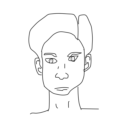
\includegraphics{graphics/im2vec/im2vec_simpletest_input_1.png}};
    \node[draw=black] at (5,0) {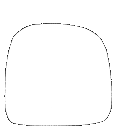
\includegraphics{graphics/im2vec/im2vec_simpletest_output_1.png}};
    \node[draw=black] at (0,5) {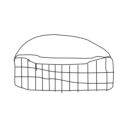
\includegraphics{graphics/im2vec/im2vec_simpletest_input_2.png}};
    \node[draw=black] at (5,5) {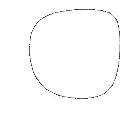
\includegraphics{graphics/im2vec/im2vec_simpletest_output_2.png}};
    \node at (0,-3) {Input};
    \node at (5,-3) {Output};
\end{tikzpicture}
    \caption{Results of Im2Vec \citep{DBLP:conf/cvpr/Reddy21} on two simple line-art sketches from \citet{eitz2012hdhso}. The image size is 128x128px.}
    \label{fig:im2vec.simpletest}
\end{figure}

However, our experiments showed that Im2Vec only works on a specific type of image, such as emojis or icons. It does not perform well when trained on line-art images, as can be seen in \Cref{fig:im2vec.simpletest}. Additionally, there were no experiments in the paper to output more than 4 shapes. It is doubtful whether it is possible to train the \gls{rnn} decoder to output the large number of bezier curves required for a clean animation frame.

The virtual sketching framework introduced by \citet{mo2021virtualsketching} is similar to Im2Vec in that it is trained without vector supervision to vectorize raster images. Other than that, it differs from Im2Vec in multiple ways. The main difference is that it constrains the output to only produce quadratic bezier curves. Also, it is an iterative model, i.e., the curves are drawn one at a time. The curves are sequentially added to a canvas in a differentiable manner. After a given number of curves is drawn, the loss is computed and propagated through all the steps. These two differences make the model more suitable for professional line art. Other differences to Im2Vec include using a different differentiable rasterizer \citep{DBLP:conf/iccv/HuangZH19a} and a finetuned perceptual loss \citep{DBLP:conf/eccv/JohnsonAF16} instead of an $L^2$ loss.
However, since the iterative model is trained mainly by computing a perceptual loss of the whole output image with the input image, the results are not semantically meaningful vector images. So while the model produces a collection of bezier curves that visually resembles the input image at a certain resolution, the vector image does not preserve the topology or meaningful structure which is necessary for clean animation frames. Related work includes ~\citet{DBLP:journals/corr/abs-2110-04830}, who use reinforcement learning as a framework for learning an iterative model in the context of comic line-art vectorization. The same constraints as with the virtual sketching framework apply here. Additionally, comic book line art does not translate well to limited animation production line art, although it would seem so at first glance.

A different approach is to incorporate parts of traditional optimization-based methods. The state-of-the-art of traditional methods was introduced by \citet{DBLP:journals/tog/BessmeltsevS19}. They attempt to detect X and T-junctions by tracing black pixel orientations with a frame field. However, additionally to the general drawbacks of traditional methods, the resulting method is not robust to more complex junctions with sharp turns, fine details or noise in general. \citet{Puhachov2021KeypointPolyvector} try to improve upon that by using a learned ensemble model to detect curve keypoints (such as junctions, start/end points and corners). Together with the input image, these keypoints are used by a geometric flow algorithm to find connections between keypoints and compute their geometry. It achieves remarkably good results, but has a more narrow aim than the proposed work. The algorithm focuses on retaining the correct stroke connectivity in the presence of noise, in their case for scanned pencil drawings. However, clean animation frames are not noisy and the curves are more narrow and densely connected, forming one large connected component for curves. Their method produces good results when applied to clean animation line art. However, resulting vector images contain overparameterized primitives and fail to vectorize more detailed and smaller shapes.

Similarly, other successful methods focus on extracting keypoints, but using a fully learned architecture. \citet{DBLP:journals/cgf/GuoZHHLW19} use a multi-task \gls{cnn} architecture to produce a centerline image and a junction image. Using this information, another \gls{cnn} extracts the curve topology. The topology image of each curve is then traced using cubic bezier least square fitting. The model is trained using raster supervision and on a synthetically created dataset. Therefore, it does not generalize well on complex real line art. Furthermore, the resulting vector image is constrained by the quality produced by the curve fitting algorithm.

On the other hand, there do exist works that attempt to fully learn a line-art vectorization model using (partially) vector supervision, which makes it easier to produce semantically meaningful vector images. \citet{DBLP:journals/tog/WangL21} use both raster and vector supervision to learn a model that generates fonts glyphs given a reference glyph. Since the number of curves required for a glyph is small ($\approx10$), the model is not trained iteratively but directly outputs a sequence of drawing commands. Their method is potentially useful, but it is doubtful whether it generalizes to a large number of curves. \citet{DBLP:journals/corr/abs-1901-03781} use solely vector supervision to reconstruct splines (which are generalizations of bezier curves). However, their approach using a hierarchical \gls{rnn} is only trained with up to three splines (with 4 to 6 control points). \citet{DBLP:conf/cvpr/BhuniaCYHXS21} use line vectorization as a self-supervised pretraining task to learn suitable sketch embeddings for downstream tasks. The line vectorization itself is similar to \citet{DBLP:conf/cvpr/Reddy21} in that it uses a \gls{cnn} as encoder and a \gls{rnn} as an encoder to generate the whole image at once. Contrary to \citet{DBLP:conf/cvpr/Reddy21} it is trained using vector supervision and constrained to output curves as a sequence of draw commands. Similar to \citet{DBLP:conf/cvpr/Reddy21}, the model is only tested with vector images containing a small number of curves.

In a similar vein, a method to generate technical drawings by \citet{DBLP:conf/eccv/EgiazarianVAVST20} is also framed as a line vectorization problem trained solely using vector supervision. It uses the Transformer architecture and is constricted to only handle 10 curves per image. To handle images with a larger amount of curves, each image is split into fixed-size tiles. The tiles are processed independently by using the Transformer model to predict vector primitives to match the curves in the image. The resulting primitives are then refined using a physics-inspired algorithm by aligning them to the black pixels in the raster image. Afterwards the primitives of all tiles are merged using a simple heuristic algorithm. While the model produces good results on technical line drawings, the authors also demonstrate that it generalizes to other line art. It is limited by the assumption that there are less than 10 curves within a tile and the reliance on the heuristic merging algorithm. The authors also show that the pure primitive predictions by the Transformer model are lacking, requiring the physics-inspired refinement algorithm, which relies on strong assumptions of the input image. This is displayed in \Cref{fig:deepvectechdraw.steps}. Additionally, the model was only tested for two vector primitives: lines and quadratic bezier curves. When applied to clean animation frames, it produces images that are both visually and structurally pretty close to the original at certain parts. However, like \citet{Puhachov2021KeypointPolyvector} it skips certain smaller and more detailed shapes. Quite paradoxically, it also produces a lot of superfluous small curves at some parts.
%Furthermore, technical line drawings do not generalize well to clean animation line art, with its more complex curves and high connectivity.

\begin{figure}
    \centering
    \begin{tikzpicture}
    \node[anchor=south west,inner sep=0] (image) at (0,0) {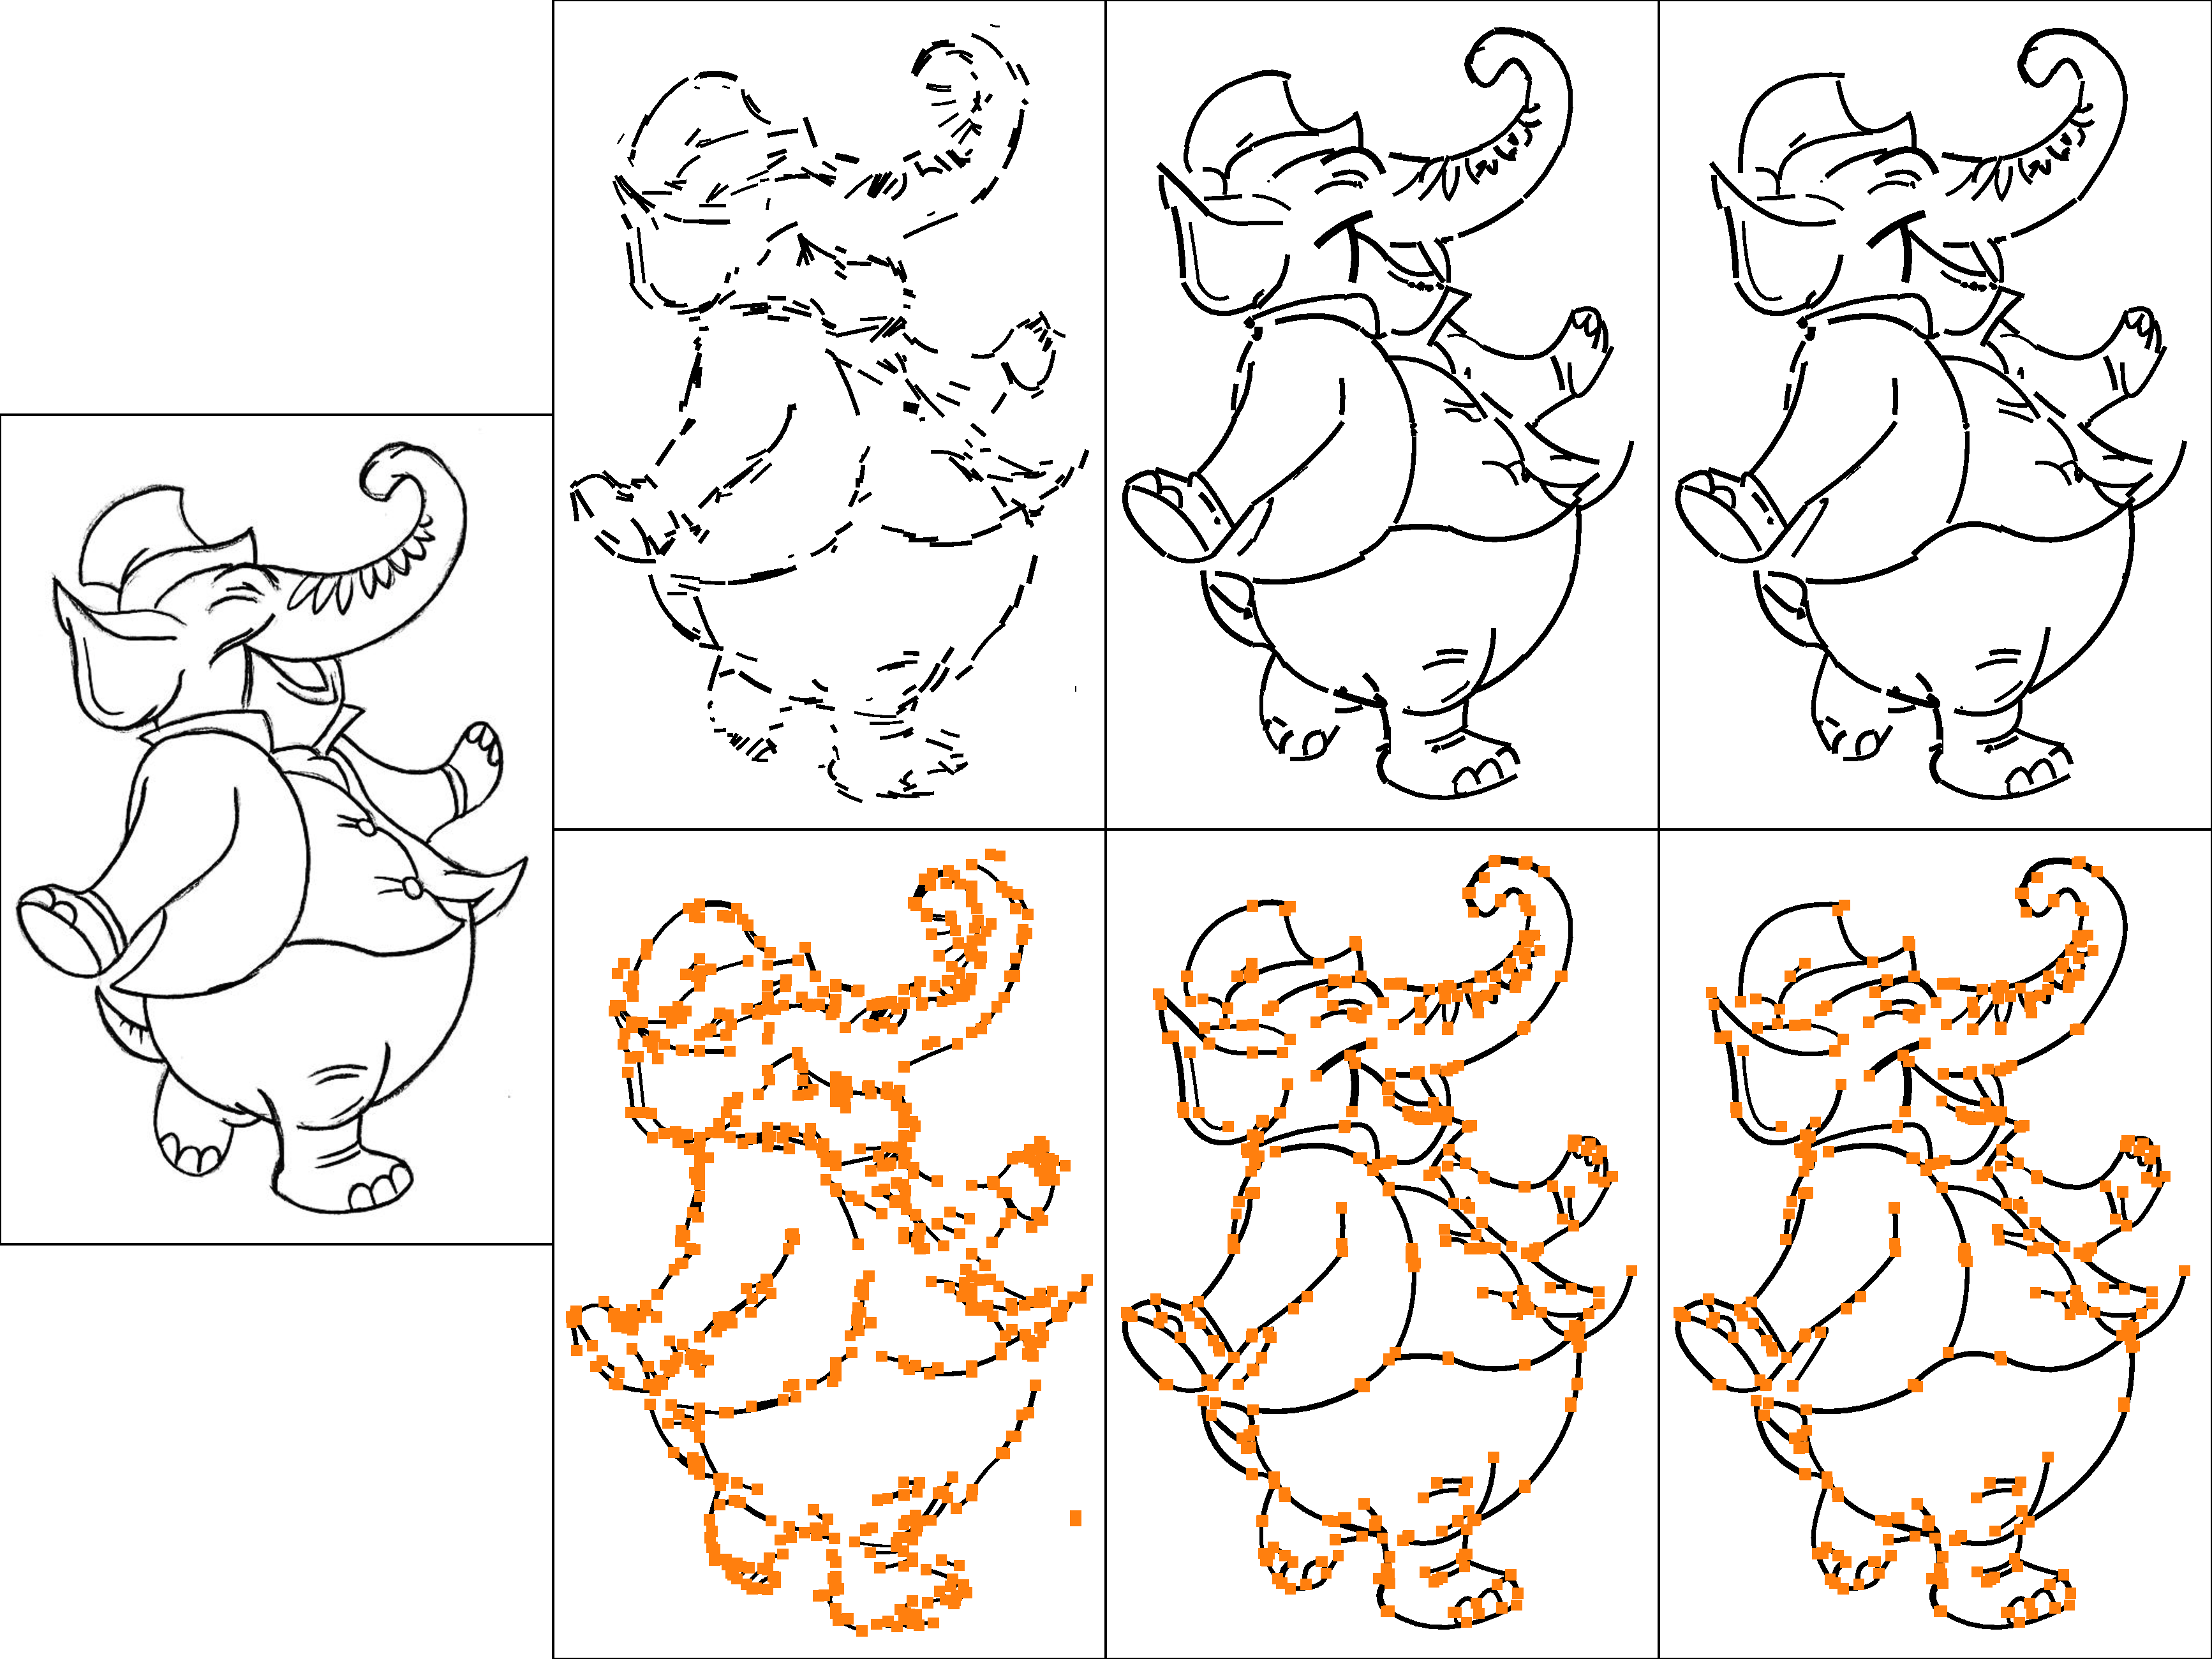
\includegraphics[width=\linewidth]{graphics/elephant.pdf}};
    \begin{scope}[x={(image.south east)},y={(image.north west)}]
        \footnotesize
        \def\y{-0.75\baselineskip}
        \def\dx{1./8}
        % Captions
        \node at (\dx,\y) [align=center] {Input};
        \node at (3*\dx, \y) [align=center] {NN};
        \node at (5*\dx, \y) [align=center] {NN + Refinement};
        \node at (7*\dx, \y) [align=center] {Full};
    \end{scope}
\end{tikzpicture}
    \caption{Result and intermediates step of the model by \citet{DBLP:conf/eccv/EgiazarianVAVST20} on line art by \citet{ivanhuska}.}
    \label{fig:deepvectechdraw.steps}
\end{figure}


\section{Cross-Domain Line-Art Vectorization}
\label{sec:crossdomain}
To our knowledge, final animation frame to clean animation frame conversion has not yet been attempted. This task is related to works attempting to generate vector line art using input images of another domain, such as photos or illustrations.

\citet{mo2021virtualsketching} provide experiments with generating vector line art using photographs as input. However, the authors concede that the model does not generalize well to complex images and produces artifacts.

The model proposed by \citet{Puhachov2021KeypointPolyvector} can be regarded as the state-of-the-art for sketch to clean vector line image conversion. However, the method relies on strong assumptions regarding the input image, specifically regarding the background-foreground threshold, which prevents the method to be used for drawings with a very noisy background (such as final animation frames).

\citet{LIPS2019} implement a GAN to generate raster contour sketch images given realistic photos as input. It is doubtful whether the results produced by this method would lead to a semantically meaningful vector image. Either way, \citet{mo2021virtualsketching} seem to outperform this method (and produce cleaner results due to the fact that the output is restricted to vector primitives).

There exists related work specifically related to anime-style illustrations. \citep{sketch} devise a model which produces a raster line art given an illustration. The results contain substantial artifacts and are therefore not quite usable as clean animation line art. The two main problems are lack of high quality training data and pixel-level supervision. The colored-sketch pair dataset normally used for such models \citep{pixiv} only superficially resembles clean animation frames, primarily since the line-art images have variable stroke widths.

\citet{Manga2021zhang} generate manga-style images from illustrations. The generation is constrained by the actual manga creation workflow. The first step of this workflow is the generation of line art given the illustration using a U-Net architecture \citep{DBLP:conf/miccai/RonnebergerFB15}. This could be used to generate a raster line art given a final animation frame. Then, the raster image could be vectorized using the line-art vectorization model. Unfortunately, the data used to train this model is not public. Furthermore, the provided results contain artifacts which will likely make it challenging to correctly vectorize the image.
\chapter{Animation Line-art Vectorization}
\label{ch:alg}

\begin{figure}
    \centering
    \begin{subfigure}{.45\textwidth}
        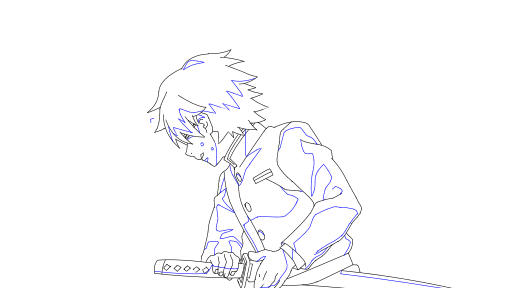
\includegraphics[width=\textwidth]{graphics/outputs/tonari-full_42.png}
        \caption{The clean animation frame in raster format as input.}
        \label{fig:tonari-42.input}
    \end{subfigure}
    \begin{subfigure}{.45\textwidth}
        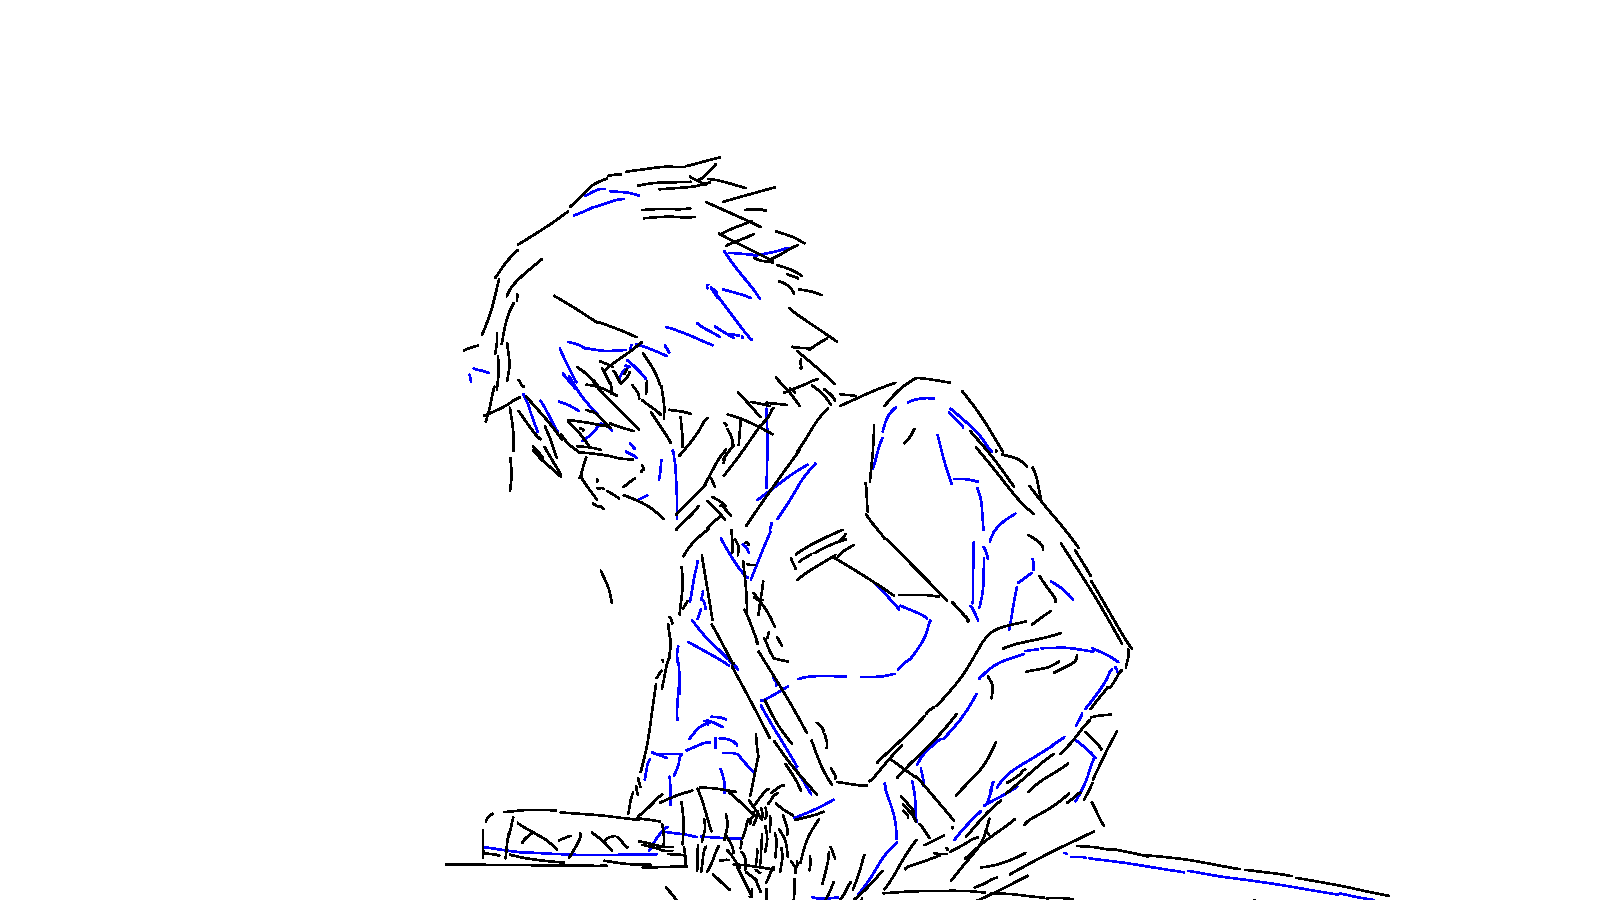
\includegraphics[width=\textwidth]{graphics/outputs/marked/512-0.512/tonari-full_42.pdf}
        \caption{The output vector image of the line-art image vectorization method.}
        \label{fig:tonari-42-output}
    \end{subfigure}
    \begin{subfigure}{.45\textwidth}
        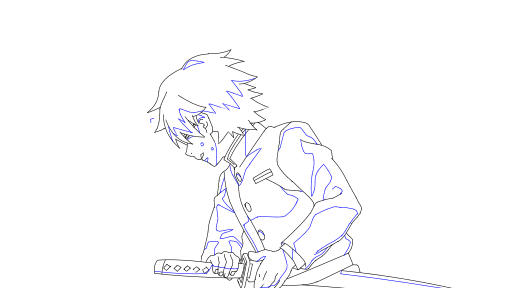
\includegraphics[width=\textwidth,trim={200px 57px 140px 175px},clip]{graphics/outputs/tonari-full_42.png}
        \caption{Region of the input image.}
        \label{fig:tonari-42.input.zoom}
    \end{subfigure}
    \begin{subfigure}{.45\textwidth}
        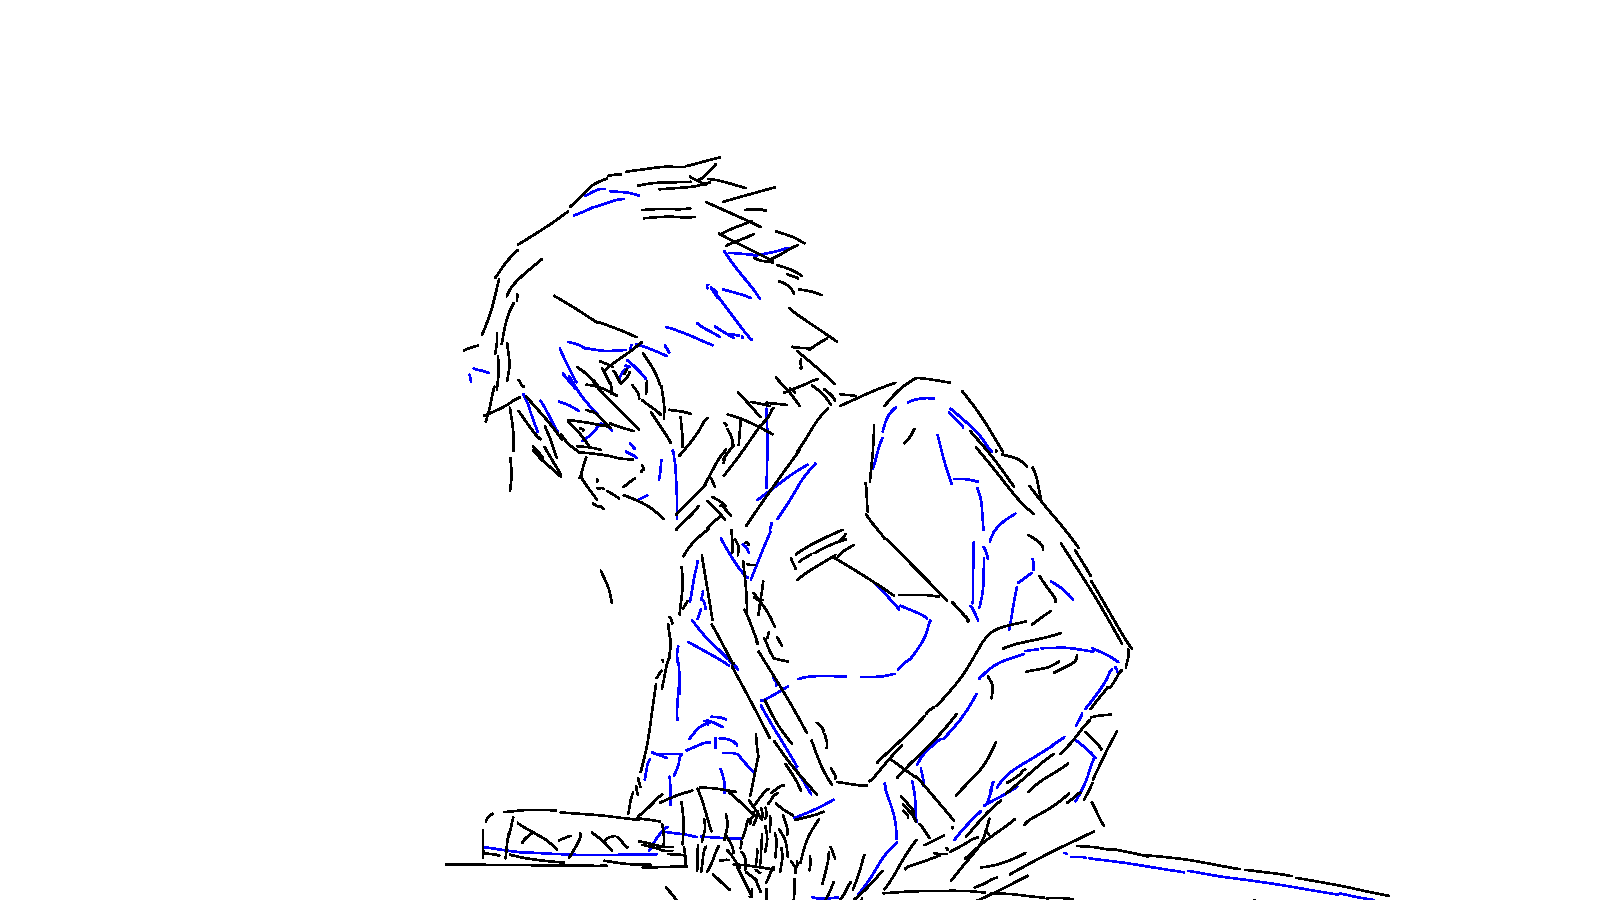
\includegraphics[width=\textwidth,trim={14em 4em 10em 12em},clip]{graphics/outputs/marked/512-0.512/tonari-full_42.pdf}
        \caption{Region of the predicted vectorization.}
        \label{fig:tonari-42-output.zoom}
    \end{subfigure}
    \caption{Sample output vector image of the developed line-art image vectorization method based on the raster clean animation frame provided by Tonari Animation as input. Zooming into the image reveals structural differences.}
    \label{fig:input.output.example}
\end{figure}

This chapter describes our work, which attempts to answer the research question posed in \Cref{sec:intro.goals}, i.e., to what extent it is possible to automatically
vectorize clean animation frame line art in a manner that is semantically meaningful. In order to answer this question, a method to automatically vectorize clean animation frame line art is developed based on previous works, which is described in \Cref{sec:model} and depicted in \Cref{fig:input.output.example}. This method is trained on a dataset detailed in \Cref{sec:dataset}. We then evaluate, both qualitatively and quantitatively, the extent to which this method and comparable works can automatically vectorize clean animation frame line art on this dataset in \Cref{sec:eval}. Finally, in \Cref{sec:ablation}, we describe alternative model architectures explored and provide an ablation study evaluating different configurations of the method.

\section{Method}
\label{sec:model}
\begin{figure}
    \centering
    \begin{subfigure}{\textwidth}
        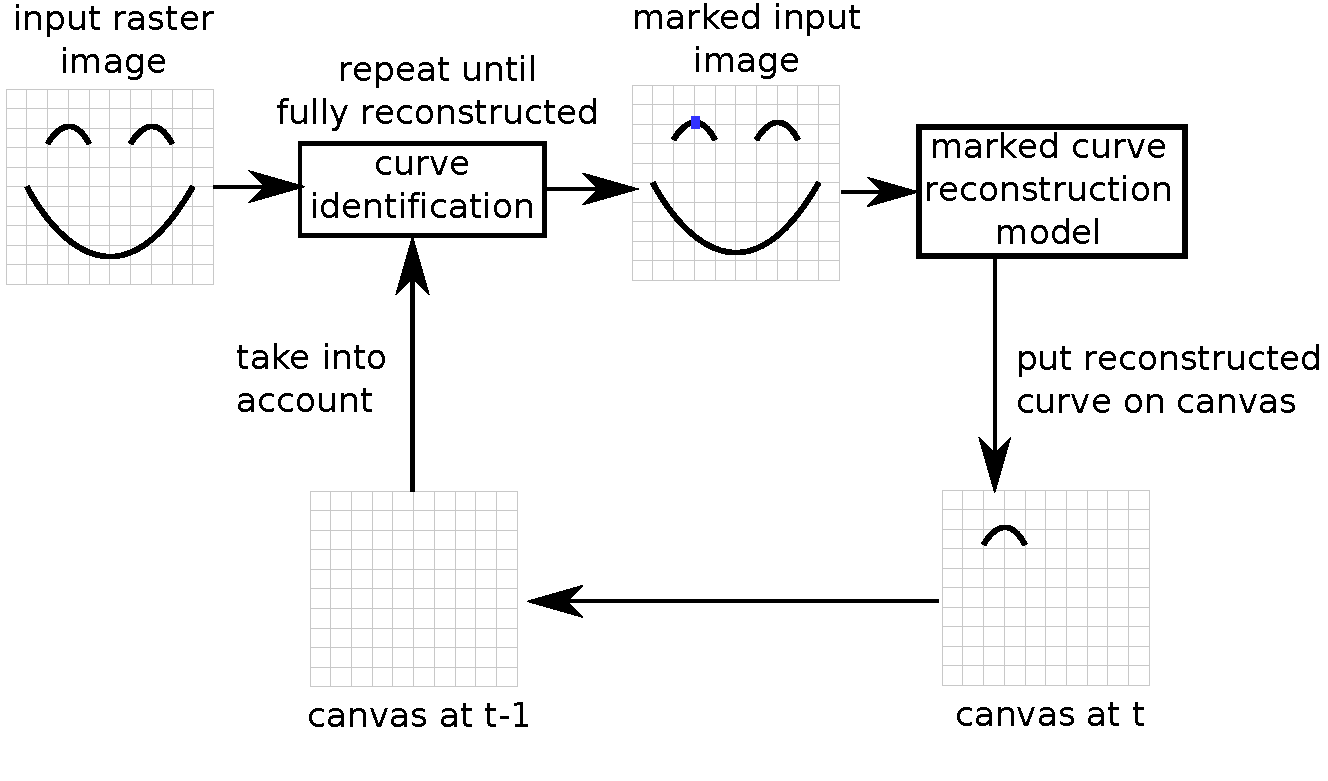
\includegraphics[width=\textwidth]{graphics/abstract_overview.pdf}
        \caption{The method unrolled at time step $t=0$}
    \end{subfigure}
    \begin{subfigure}{\textwidth}
        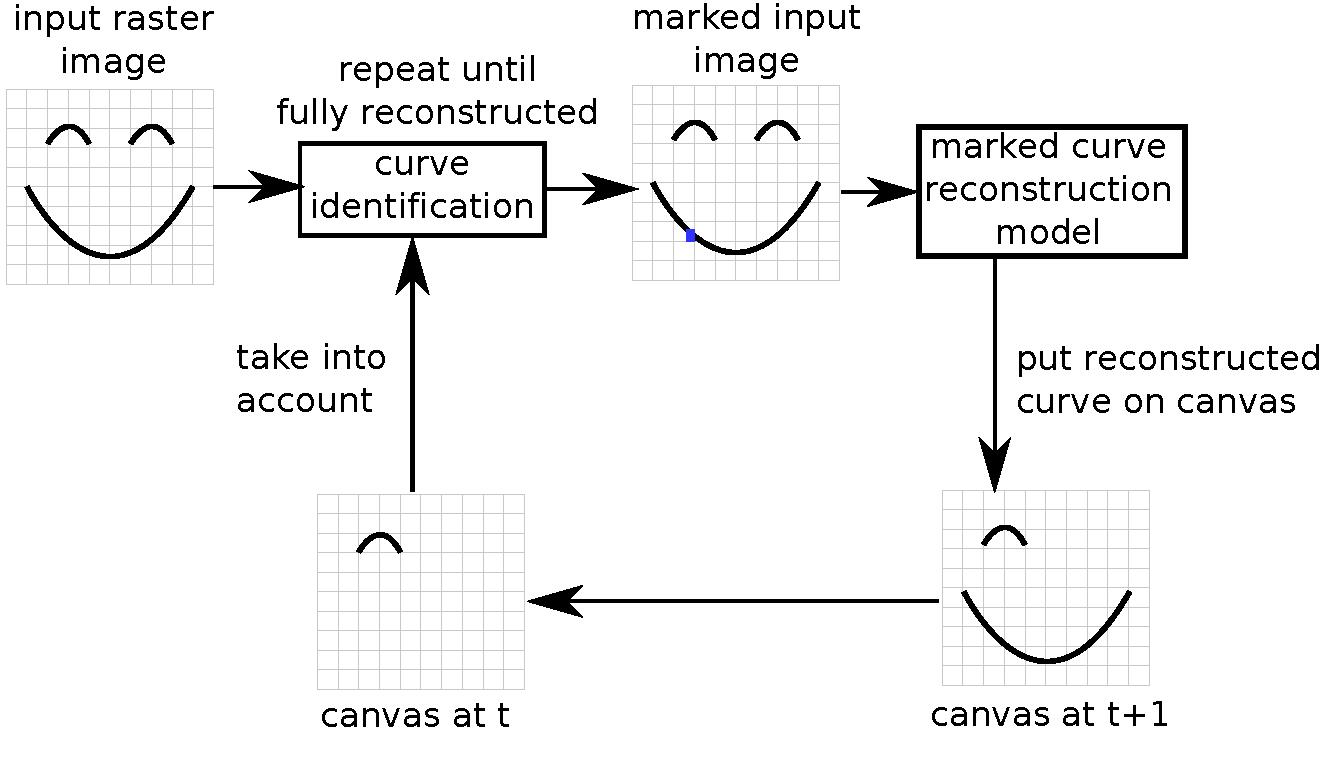
\includegraphics[width=\textwidth]{graphics/abstract_overview_2.pdf}
        \caption{The method unrolled at time step $t+1$}
    \end{subfigure}
    \caption{Overview of the proposed method. The method iteratively reconstructs a given raster line-art image as a vector image. At time step $t=0$, an algorithm identifies a new curve to reconstruct and places a marker on it. This information is then passed to a learned marked-curve reconstruction model to reconstruct the curve in vector format using cubic bezier curve parameters. This output is added to a canvas, which is taken into account when identifying the curve to reconstruct at $t+1$.}
    \label{fig:model.arch}
\end{figure}

In this section we describe a method to automatically convert line-art raster images into vector images. The method is visualized in \Cref{fig:model.arch} and consists of two parts: the main part is a learned model that takes as input a raster line-art image and a mark on a curve in this image and outputs a cubic bezier curve which fits the marked curve. The second part is a lightweight algorithm that uses this model iteratively to reconstruct all curves in an image. The marked-curve reconstruction model is described in \Cref{subsec:model.arch}, while the iterative curve reconstruction algorithm is described in \Cref{subsec:model.infer}.

To motivate this architecture, recall that a line-art image consists of a set of bezier curves. The amount of bezier curves is considerably large (see \Cref{sec:dataset}). Following this, the task of line-art image vectorization is decomposed into two non-trivial sub-tasks:
%
\begin{itemize}
    \item curve identification: given a line-art raster image and an image of already reconstructed curves (i.e., a \textit{canvas} image), sample a point that lies on a curve (i.e., a \textit{marker}), and
    \item curve reconstruction: given a line-art raster image and a point lying on a curve (i.e., the marker), reconstruct the marked curve.
\end{itemize}
%
Decomposing the task into these two subtasks with a more narrow objective reduces the space of possible solutions of the algorithm, thereby aiding the design of the algorithm. Furthermore, this architecture allows the curve reconstruction and identification to be independent of the number of curves, further decreasing the solution space. Additionally, this structure is more amenable to manual fixing of the output (as described in \Cref{sec:challenges,subsec:cleanframes}), since missing curves can easily be reconstructed by invoking the curve reconstruction part with a marker on the curve in question.

Of the two subtasks, curve reconstruction is the more complex part and is handled by the learned marked-curve reconstruction model introduced in \Cref{subsec:model.arch}. On the other hand, curve identification is considerably easier to solve for the data primarily considered in this work (i.e., clean line-art raster images). The curve identification algorithm is described as part of the iterative curve reconstruction algorithm in \Cref{subsec:model.infer} and simply samples a pixel belonging to a curve of a grayscale line-art raster image. Since the background is white and the curves are colored, this pixel will be black (i.e., closer to 0 than to 1) in a grayscale version of the line-art image. Notice that this curve identification algorithm is both tailored to clean line-art images and not differentiable. Hence, if the input image is in a different domain or a fully differentiable algorithm is needed (such as in the cross-domain line-art image vectorization proposed as an extension of this work in \Cref{sec:challenges}), it is necessary to replace the proposed curve identification algorithm with a more suitable alternative. While this is an orthogonal problem, \Cref{subsec:model.infer} also describes a potential alternative.

\subsection{Marked-Curve Reconstruction Model}
\label{subsec:model.arch}

This section details the architecture of the marked-curve reconstruction model, which is depicted in \Cref{fig:marked.model.arch}. The model takes as input a line-art raster image with a mark placed on a curve in it, and outputs the bezier curve parameters fitting the marked curve. This model was designed by following the principle that reducing the complexity of the task the model needs to solve increases the probability that the model actually converges to a suitable state. As an example of a widely used model architecture that follows this principle, diffusion models \citep{DBLP:conf/icml/Sohl-DicksteinW15,DBLP:conf/cvpr/RombachBLEO22} attempt to accomplish image generation by iteratively taking small denoising steps instead of generating the whole image at once.

This is achieved by three design decisions. The most important design decision is to have the model reconstruct only a \textit{single} curve instead of all curves per invocation. Since the amount of curves in clean frame images is quite high (see \Cref{sec:dataset}), this significantly reduces the space of possible solutions of the model. The other two decisions are based on the input and the output of the model and are explained below.

\subsubsection{Input and Output}
\label{subsec:io}

The input of the model is a line-art raster image. Additionally, this image contains one pixel of a different color from the curves and the background lying on a curve. This pixel is the marker indicating which curve to reconstruct. Importantly, this means that the \textit{location} of the curve is already established. This information can be used to reduce the task complexity for the model by centering the input image on the mark. This way, the model can be trained on the assumption that the center pixel has to lie on the reconstructed curve, avoiding the need for the model to learn to reconstruct the curve at the correct location. Furthermore, note that the centering of the input image on the mark obviates the need to provide the mark location explicitly to the model, since it will be on the center for all input images and is thus implicitly provided. This includes both appending the mark location to the input vector and displaying the mark using a different color on the input image. Hence, the depiction of the mark in the raster image is kept purely for illustrative purposes.

The raster input images are represented using the \gls{rgb} color model, i.e., each pixel is represented using three numbers in $[0,255]$. In order to not let multiplications and gradients in the architecture explode, the numbers are divided (i.e., scaled) by the maximum 255 to be in $[0,1]$. Furthermore, the model is trained and evaluated using clean line-art images only, i.e., images which can be binarized into black and white images, where the curves are black and the background is white. These images could be represented using a single color channel per pixel, which would slightly reduce the model size. However, as there was no difference in model performance between \gls{rgb} and monochrome input images, the input images are kept in \gls{rgb} format. This way, no assumption of monochrome input images is baked into the model and it can also handle non-monochrome input images.

The output of the model is defined as the parameters of a cubic bezier curve with a fixed stroke width. The parameters are defined by the start point, the end point and two control points, resulting in a vector of length 8. This output structure is sufficient to represent the output data domain considered in this work, i.e., clean animation frames. Recall that clean frames consist of quadratic and cubic bezier curves with fixed stroke width of predefined colors, as described in \Cref{subsec:cleanframes}. Furthermore, the restrictive nature of the output structure reduces the task complexity in three ways. Firstly, the model does not need to learn to use different primitives other than the cubic bezier curve. This can be achieved since clean frames only consist of quadratic and cubic bezier curves, and the possibility of representing quadratic bezier curves as cubic bezier curves. Secondly, the model does not need to learn the correct stroke width of the reconstructed curve, since it is a constant that can be defined for the whole image. Thirdly, the model does not need to learn the correct color of the reconstructed curve, since color follows a predefined schema that can be handled by preprocessing the image.

\subsubsection{Model Architecture}

\begin{figure}
    \centering
    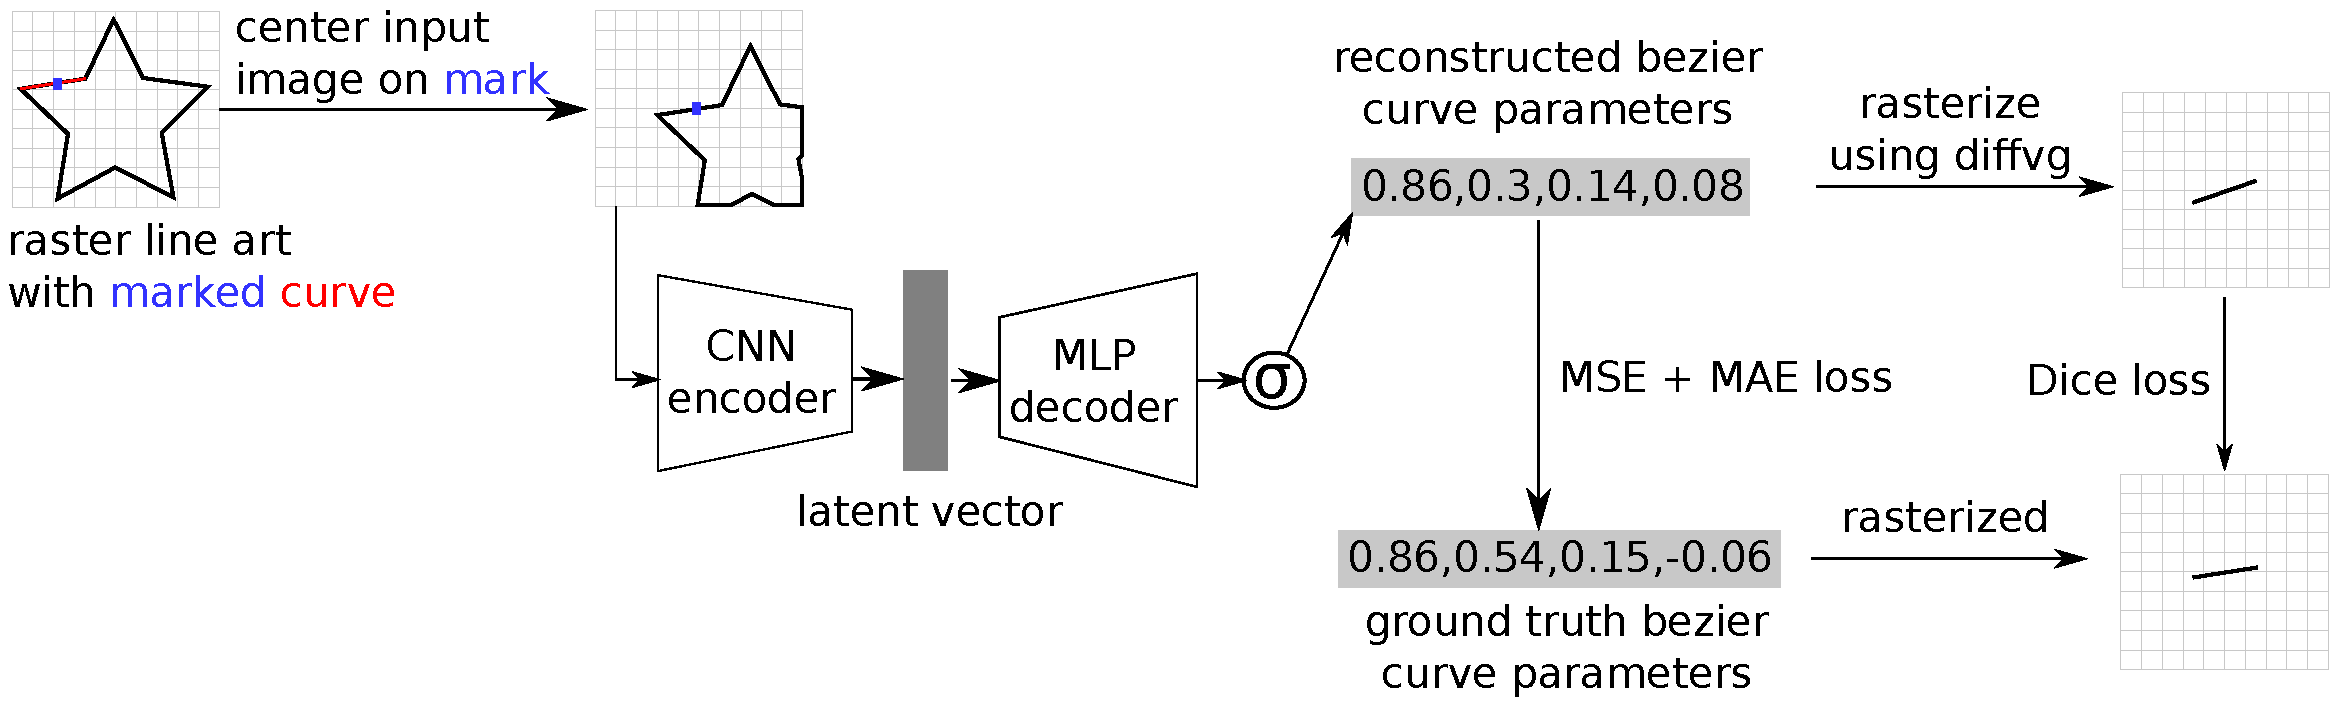
\includegraphics[width=\textwidth]{graphics/mcrm.pdf}
    \caption{Architecture overview of the marked-curve reconstruction model. Note that for brevity, lines with two points are shown instead of cubic bezier curves with four points.}
    \label{fig:marked.model.arch}
\end{figure}

The architecture of the marked-curve reconstruction model is depicted in \Cref{fig:marked.model.arch}. Due to the nature of the task requiring the model to generate complex output based on high-dimensional input, it is designed as an encoder-decoder architecture. That is, it consists of an encoder neural network that turns the input image $\mathbf{x}$ into a latent vector $\mathbf{z}$ of predefined length $L$, and a decoder neural network that turns this latent vector into cubic bezier curve parameters $\mathbf{o}$. In general, the model is designed to be as small and simple as possible and follows standard practices. Note that a small model size has considerable benefits, such as faster computation and less memory requirements, while aiding regularization (see \Cref{subsec:bg.nn.reg}).

Since the input is an image, the encoder is a convolutional neural network. As described in \Cref{subsec:bg.cnn}, convolutional layers have an inductive bias for images. Furthermore, they are locally connected to the input and therefore work for varying input image sizes (i.e., resolutions). The encoder consists of 6 blocks, where each block is formed by a 2-dimensional convolutional layer, followed by 2-dimensional batch normalization and \gls{relu} activation. The architecture is designed following standard practices such that the image size is halved and the channel size is doubled at every convolutional layer.

A disadvantage of using stacked convolutional layers is that the output is a 3-dimensional matrix, which does not satisfy the structure needed as latent vector to be input to the decoder. In order to arrive at a latent vector of predefined length $L$ independent of the input image size, the global pooling technique (see \Cref{p:pooling} is used). That is, the last convolutional layer has a filter size corresponding to the latent vector length $L$. Following this, a global average pooling layer is used to reduce the space dimensions of the resulting output, leading to a 1-dimensional latent vector of length $L$.

The hyperparameters of the encoder layers are displayed in \Cref{tab:encoder.summary}. Each convolutional layer doubles the filter size of the previous layer and has a stride of 2 and a padding of 1. The last convolutional layer has a stride of 1. Note that the batch normalization following each convolutional layer is not displayed. They follow the same size as their preceding convolutional layer output and are parameterized with $\epsilon=10^{-5}$ and a momentum of $\mu=0.1$.

Note that, as described above, the encoder architecture is designed to handle variably sized input, with these variables being denoted in \Cref{tab:encoder.summary}. The batch size $B$ is used to process multiple observations in parallel and increase the effectiveness of batch normalization by decreasing the variance (see \Cref{subsec:bg.nn.batchnorm}). The image width $W$ and height $H$ need to be a multiple of 2, but can be otherwise freely chosen. The latent vector length $L$ needs to correspond to the length used for the input vector of the decoder. For this work, the hyperparameters are set to $B=32$,  $W=H=512$ and $L=128$. Note that the width and height do deliberately not correspond to the exact resolution of clean animation frames in the dataset (see \Cref{sec:dataset}). This is done to show that the model does not overfit to a specific resolution. As an aside, \glspl{cnn} are typically trained on significantly smaller $W$ and $H$ \citep{DBLP:conf/cvpr/HeZRS16}, especially when trained for image classification. However, these small image resolutions would compress the clean animation frame beyond a reasonable possibility of detecting individual curves.

\begin{table}[h]
    \centering
    \begin{tabular}{c|l|r|r|r|r|r}
         layer & output shape & \# params & filter size & kernel size & stride & padding \\
         \hline
         2-d conv & ($B$, 32, $W/2$, $H/2$) & 896 & 32 & 3 & 2 & 1 \\
         2-d conv & ($B$, 64, $W/4$, $H/4$) & 18496 & 64 & 3 & 2 & 1 \\
         2-d conv & ($B$, 128, $W/8$, $H/8$) & 73856 & 128 & 3 & 2 & 1 \\
         2-d conv & ($B$, 256, $W/16$, $H/16$) & 295168 & 256 & 3 & 2 & 1 \\
         2-d conv & ($B$, 512, $W/32$, $H/32$) & 1180160 & 512 & 3 & 2 & 1 \\
         2-d conv & ($B$, $L$, $W/32$, $H/32$) & 589952 & $L$ & 3 & 1 & 1 \\
         avg pool + squeeze & ($B$, $L$) & 0 & $L$ & $W/32$ & - & - \\
    \end{tabular}
    \caption{Summary of the layers of the encoder neural network of the marked-curve reconstruction model.}
    \label{tab:encoder.summary}
\end{table}

The decoder is a 2-layer \gls{mlp}, which turns the latent vector of length $L$ into a vector of length $P*2$, where $P$ is the number of cubic bezier curve parameters. Since cubic bezier curves are parameterized by a start point, an end point and two control points, $P=4$. With only one hidden layer, the decoder is as shallow as possible. The hidden layer is introduced to enable the decoder to learn non-linear transformations of the latent vector. It is followed by batch normalization, which is parameterized with $\epsilon=10^{-5}$ and a momentum of $\mu=0.1$ as in the encoder and a \gls{relu} activation. The output layer outputs a vector of length $2P$. Intuitively, this could directly be used as output. However, these numbers are unbounded and could theoretically go towards $\infty$. Hence, the output is restricted to $[0,1]$ using the sigmoid activation function (see \Cref{eq:sigmoid}). The x coordinates of the cubic bezier curve points are then scaled with the image width, while the y coordinates are scaled with the image height.

\begin{table}[h]
    \centering
    \begin{tabular}{c|l|r|r}
         layer & output shape & \# params & size  \\
         \hline
         linear & ($B$, $L/2$) & 8256 & $L/2$  \\
         batch norm & ($B$, $L/2$) & $2(L/2)$ & \\
         \gls{relu} & ($B$, $2P$) &  &  \\
         linear & ($B$, $2P$) & 520 & $2P$  \\
         sigmoid & ($B$, $2P$) & 520 &  \\
    \end{tabular}
    \caption{Summary of the layers of the encoder neural network of the marked-curve reconstruction model.}
    \label{tab:decoder.summary}
\end{table}

\Cref{tab:encoder.summary,tab:decoder.summary} show the numbers of learnable parameters of the model. In total, the model has 2,169,672 learnable parameters. The distribution of these learnable parameters indicates that the model is encoder-heavy, with a large portion of them assigned to the convolutional layers. Since the encoder does the heavy lifting, more complex encoder architectures such as the ResNet \citep{DBLP:conf/cvpr/HeZRS16} and ConNeXt \citep{DBLP:conf/cvpr/0003MWFDX22} were tried as alternatives. For these architectures, encoder weights which were pretrained on larger image datasets such as ImageNet \citep{ILSVRC15} are available, obviating the need to train an encoder from scratch. However, they did not perform significantly better than the simple encoder architecture introduced here. Hence, they are not used in order to keep the model as small and simple as possible.


\subsubsection{Training}
\label{subsubsec:model.training}

The model is trained to generate a curve that resembles the ground truth (i.e., the gold standard) curve both visually and in its semantic topology. For this reason, a combination of a raster-based loss for visual similarity and a vector-based loss for semantic correctness is used to train the model. Intuitively, the raster-based loss is used to optimize the model to output a curve that covers the pixels of the original line as closely as possible. The vector-based loss is then used to optimize the model to output semantically correct curve parameters. Furthermore, the vector loss is multiplied with a weight of 100 to not let the raster-based loss dominate the combined loss. This task-derived loss combination is an important distinction from related work \citep{DBLP:conf/cvpr/Reddy21,mo2021virtualsketching,DBLP:conf/eccv/EgiazarianVAVST20}.

The vector loss follows \citep{DBLP:conf/eccv/EgiazarianVAVST20} and is an even combination of \gls{mae} and \gls{mse}. It is defined in \Cref{eq:model.loss}, where $\mathbf{o}$ is the model output, $\mathbf{y}$ are the ground truth cubic bezier curve parameters and $L_1$ and $L_2$ are defined in \Cref{eq:mae,eq:mse}, respectively. The loss is closely related to the Huber loss defined in \Cref{eq:huber}. Intuitively, since the \gls{mae} and the \gls{mse} have their advantages and disadvantages, the loss simply uses both using the same weight (see \Cref{p:losses.regression}).

\begin{equation}
    \label{eq:model.loss}
    L(\mathbf{o},\mathbf{y})=0.5*L_1(\mathbf{o},\mathbf{y})+0.5*L_2(\mathbf{o},\mathbf{y})
\end{equation}

Defining a raster-based loss is more difficult, since the model outputs the cubic bezier curve in vector format, which needs to be rasterized. As described in \Cref{subsec:bg.vector}, rasterization is trivial and can be done deterministically. However, for the loss it is crucial that the rasterization is differentiable (see \Cref{subsec:bg.nn.optim}). Hence, the differentiable rasterizer introduced by \citet{Li:2020:DVG} is used to rasterize the cubic bezier curve parameters. This raster output image is then compared to the raster input image, with all curves aside from the marked curve removed.

A typical choice for comparing two raster images is to simply use the \gls{mse} (or, less commonly the \gls{mae}). However, the rasterized curve image exhibits a significant class imbalance, since most of the image is white with only the curve being black. Hence, as described in \Cref{p:dice.loss}, the dice loss defined in \Cref{eq:dice} is a better choice than \gls{mse}. Accordingly, the performance of the model is evaluated using the \gls{iou} defined in \Cref{eq:iou} of the output and the ground truth curve raster image.

The model is trained using the widely used Adam \citep{DBLP:journals/corr/KingmaB14} optimizer with a learning rate of $\eta=5*10^{-4}$. The other hyperparameters are set to the default PyTorch \citep{Paszke_PyTorch_An_Imperative_2019} values, i.e., no weight decay, $\beta_1=0.9$, $\beta_2=0.999$ and $\epsilon=1*10^{-8}$.

\begin{figure}
    \centering
    \begin{subfigure}{.45\textwidth}
        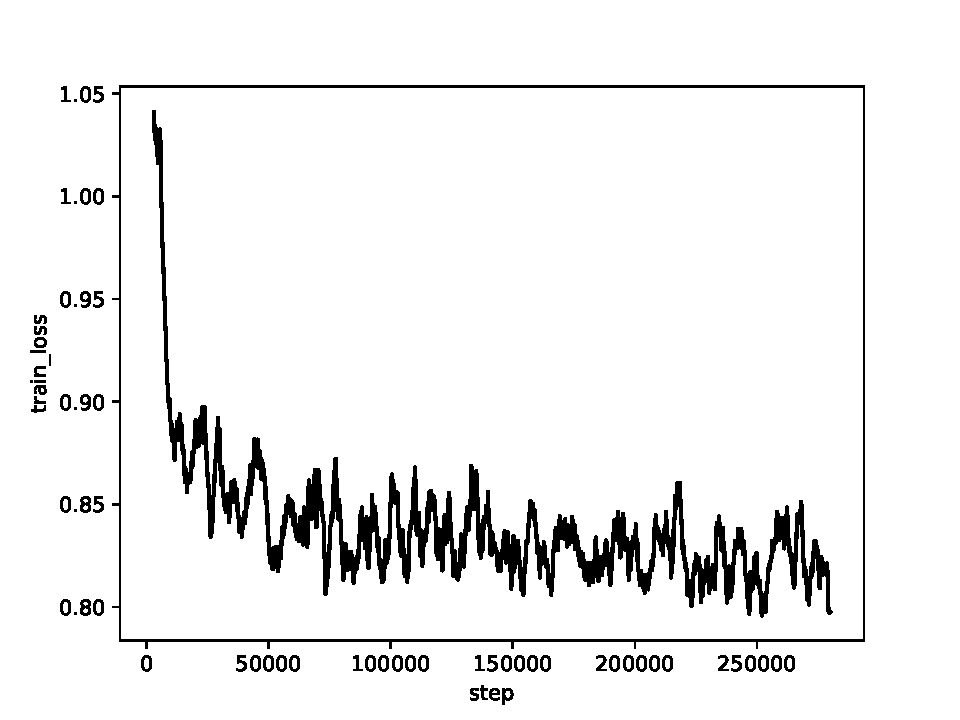
\includegraphics[width=\textwidth]{graphics/work-artifacts/marked/server/train_loss.pdf}
        \caption{The training loss.}
    \label{fig:model.train.progress.loss}
    \end{subfigure}
    \begin{subfigure}{.45\textwidth}
        \includegraphics[width=\textwidth]{graphics/work-artifacts/marked/server/val_iou_step.pdf}
        \caption{The validation single curve \gls{iou}.}
    \label{fig:model.train.progress.iou}
    \end{subfigure}
    \caption{Training progress of a model measured using the loss on the training dataset and the single curve \gls{iou} on the validation dataset per iteration.}
    \label{fig:model.train.progress}
\end{figure}

To visualize the training process, figure \Cref{fig:model.train.progress.loss} shows the loss per iteration, where one iteration indicates one batch of the data being processed. After all batches are processed, the training continues again starting from the first batch. The batch size is set to $B=32$, which is the largest size possible given available dedicated \gls{gpu} memory. \Cref{fig:model.train.progress.iou} shows the performance of the model on the validation dataset provided by Tonari Animation (described in \Cref{sec:eval.setup}). The performance is measured using the \gls{iou} of one reconstructed curve and the ground-truth curve (see \Cref{subsec:ablation.limitation}). It converges to a single curve \gls{iou} of 0.62.

\subsection{Iterative Curve Reconstruction Algorithm}
\label{subsec:model.infer}

\begin{figure}
    \centering
    \includegraphics[width=\textwidth]{graphics/icra.pdf}
    \caption{Overview of the iterative curve reconstruction algorithm. This overview goes into more detail regarding the curve identification and reconstruction than \Cref{fig:model.arch}.}
    \label{fig:icra}
\end{figure}

The marked-curve reconstruction model introduced in \Cref{subsec:model.arch} is the main part of the line-art image vectorization method, but reconstructs only a single curve without color or stroke width information given a marked curve on the line-art raster image. In order to vectorize an entire line-art raster image, an algorithm has to be defined around the model that performs three tasks: 

\begin{enumerate}
    \item handles color (and stroke width) information,
    \item given the input image and a canvas of already reconstructed curves, computes markers identifying curves to reconstruct, and
    \item invokes the marked-curve reconstruction model using the input image and a marker of an identified curve and places the output on the canvas.
\end{enumerate}

The algorithm is depicted in \Cref{fig:icra} and explained in the following.

\subsubsection{Color and Stroke Width}
\label{subsubsec:colorstroke}

For the first task, recall that the marked-curve reconstruction model does not output color information. Since color carriers significant meaning in clean frames (see \Cref{subsec:cleanframes}), it is necessary for the algorithm to produce the correct color information for all predicted curves. This can be done using simple pre-processing and post-processing steps, which both reduces the task complexity of the model and ensures that the output is correct.

In detail, note that the color schema of clean animation frames is known a priori, as defined in \Cref{fig:bg.color-schema}. Hence, it is possible to segment the input image according to these colors (see \Cref{subsubsec:classification}). \Cref{fig:segment.ex} exemplifies this. Then, the curve colors of each segment are set to black and each segment is individually input into the marked-curve reconstruction model. The output of the marked-curve reconstruction model contains no color information, but since the true color of the segment is known, the color of the output can be set to the segment color.%Note, that, in order to provide consistent comparability, all input and output images of the method are displayed using black curves unless otherwise noted.

In the same vein, the marked reconstruction model does not output stroke width information. However, since all curves in a clean animation frame share the same stroke width, it suffices to define one constant stroke width for the input image and to apply this to all reconstructed curves. The stroke width can either be defined by the user or inferred from the input image.

\begin{figure}
\begin{subfigure}{.5\textwidth}
    \includegraphics[width=\textwidth]{graphics/douga/49.pdf}
    \caption{Full clean animation frame.}
    \label{fig:segment.ex.full}
\end{subfigure}%
\begin{subfigure}{.5\textwidth}
    \includegraphics[width=\textwidth]{graphics/douga/49_black.pdf}
    \caption{Black segment of the clean animation frame.}
\end{subfigure}
\begin{subfigure}{.5\textwidth}
    \includegraphics[width=\textwidth]{graphics/douga/49_blue.pdf}
    \caption{Blue segment of the clean animation frame.}
\end{subfigure}%
\begin{subfigure}{.5\textwidth}
    \includegraphics[width=\textwidth]{graphics/douga/49_red.pdf}
    \caption{Red segment of the clean animation frame.}
\end{subfigure}%
    \caption{Example of a clean animation frame provided by Tonari Animation segmented by color.}
    \label{fig:segment.ex}
\end{figure}

\subsubsection{Curve Identification}
\label{subsubsec:curve.ident}

In order to indicate to the marked-curve reconstruction model which curve needs to be reconstructed, the second task consists of sampling a pixel lying on a curve not already reconstructed given the input image (more specifically an input image segment, as described in \Cref{subsubsec:colorstroke}) and a canvas image containing already reconstructed curves. In the case of clean line-art images considered in this work, this can simply be done by sampling a random black pixel, where a pixel is considered black if it is closer to 0 than to 1. This pixel is guaranteed to lie on a curve. As an aside, a potential improvement to this algorithm is to always sample the pixel from the largest contiguous area of black pixels, in order to reconstruct the longest curves first. However, this has not been implemented in order to keep the algorithm as simple as possible.

In order to ensure that only curves that have not yet been reconstructed are identified, the canvas image is subtracted from the input image whenever a new curve is added to the canvas and before the marker pixel is sampled. This also helps the marked-curve reconstruction model to not output duplicate curves.

Both the curve identification by sampling black pixels and the subtraction of the canvas image from the input image have the assumption of clean line-art images. Thus, when the line-art vectorization is applied to input images of different domains, these two parts have to be adapted. If there exists a binarization algorithm of considerable quality for this domain (e.g. \citet{DBLP:conf/das/SuLT10}), then simply binarizing images with this algorithm will suffice. Otherwise, one alternative is to train a curve identification model. This alternative would render the entire line-art image vectorization method end-to-end differentiable. The curve identification model would take as input both the input line-art image and the canvas image, where the latter could be appended as a fourth color channel to the former. The output would a vector containing two elements, constrained by the sigmoid function to lie in $[0,1]$, indicating the coordinates of the marker. Then, the architecture would be a convolutional neural network with global average pooling on a filter size of 2 at the end. There are multiple candidates for loss functions. One possibility is to calculate the distance of the marker to all ground truth curves that are not present in the canvas image and taking the minimum. This would require the training images to also be available in vector format.

\subsubsection{Marked-Curve Reconstruction Model Invocation}
\label{subsubsec:model.invok}

In order to vectorize the entire line-art image, the marked-curve reconstruction model has to be invoked iteratively until all curves are reconstructed. This is done in multiple steps, which are laid out in \Cref{alg:iterative.recon}. In this algorithm, the remaining image is the raster image containing curves that are not yet reconstructed. The canvas image is stored as vector image using the \gls{svg} format. It is rasterized when being used to update the remaining curves image.


\begin{algorithm}
  \caption{Iterative Curve Reconstruction.}
  \label{alg:iterative.recon}
  \KwIn{A raster line-art image.}
  \KwOut{A vector line-art image.}
  Segment input image by color\;
  \ForEach{image segment}
  {
  canvas = an empty vector image of the same size as the input image\;
  remaining = image segment\;
  \While{number of black pixels in remaining > $T$;}
  {
  Compute marker by applying curve identification on the remaining image\;
  Centered image = center the remaining image on the marker\;
  reconstructed curve = invoke the marked-curve reconstruction model using the centered image\;
  Inverse the center location of the curve by using the mark location\;
  Add the reconstructed curve to the canvas image\;
  remaining = remaining - rasterized canvas image\;
  }
  Set color of all curves in the canvas image to the segment color\;
  }
  Merge the canvas images\;
  \Return{Merged canvas images}
\end{algorithm}

Note, that Line 5 in \Cref{alg:iterative.recon} constitutes an intuitive stopping criterion enabled by the progressive canvas image subtraction from the remaining image. The curve reconstruction is iteratively applied until the number of black pixels (i.e., the number of possible markers) in the remaining image is greater than some threshold $T$. If the curve identification and reconstruction worked perfectly, the difference between the rasterized canvas image and the remaining image would reach 0 at some point. In this case, the threshold should be set to $T=1$. However, since errors in the reconstructed curves are to be expected, there will remain a number of black pixels that are part of an already reconstructed curve that does not fully cover the curve in the input image. Repeatedly invoking the marked-curve reconstruction model on such pixel artifacts will lead to worse results. Since missing a few curves is not a significant issue, it is tolerable to set the threshold to a low number of black pixels greater than 1. For this algorithm, the threshold is set to $T=\lfloor B*0.1 \rceil$, where $B$ is the number of black pixels in the original image.

\subsubsection{Advantages and Limitations}
\label{subsec:method.limitations}

The theoretical runtime complexity of the algorithm as defined in \Cref{alg:iterative.recon} is in $\mathcal{O}(p)$, where $p$ is the number of black pixels in the input image, which is connected to the number of curves $n$. As the performance of the marked-curve reconstruction model increases, the runtime will be approximately linear in $n$. However, it is possible to significantly reduce the runtime  by processing a batch of curves $b<n$ concurrently, instead of one curve at a time. For this, the curve identification algorithm described in \Cref{subsubsec:curve.ident} can be adapted to sample $b$ black pixels instead of a single black pixel. To decrease the probability of multiple marks belonging to the same curve being sampled, the image should be divided in $b$ patches, with a single mark being sampled in each patch. The marked-curve reconstruction model does not need to be adapted, since it possesses the ability to processes a batch of inputs, which is already done at training time. Note that this adaptation increases the memory requirement by roughly $b$ times. However, since the test dataset is rather small (see \Cref{sec:dataset}), this parallel version of the algorithm has not been implemented.

Furthermore, an advantage of this algorithmic structure is that it significantly eases the effort required to manually fix an output image. While identification of missing curves is a trivial task for humans, fixing wrongly reconstructed curves is tedious. Following this, the algorithm is designed to maximize the former in lieu of the latter. On the one hand, it allows to post-hoc reconstruct curves that were missed by the first run of the algorithm without affecting the rest of the output by simply placing a mark on a random point of the curve in question and invoking the marked-curve reconstruction model. On the other hand, by letting the learned model focus on reconstruction of a single curve, its reconstruction results will be at least better than a model that needs to perform reconstruction and identification of all curves, thereby reducing the need to fix reconstructed curves.

Lastly, there are two issues associated with overlapping curves, i.e., pixels which are part of multiple curves. Firstly, this directly affects the iterative curve reconstruction algorithm. Suppose the marked-curve reconstruction model outputs one of the multiple overlapping curves, then this curve will be placed on the canvas image and removed from the input image. In this process, the overlapping pixels will also be removed, leaving behind a hole in the remaining curves, effectively splitting them. Hence, if the hole is large enough, the curve reconstruction model will reconstruct only one part of the split curve instead of the whole curve. Secondly, the curve reconstruction model will receive ambiguous information on which curve to reconstruct during training in these cases, hampering its ability to derive meaningful gradients at all in the worst case. However, both of these issues are negligible since the amount of overlapping curves is small, as the calculation in \Cref{sec:dataset} shows.


\section{Dataset}
\label{sec:dataset}

The dataset used to train and evaluate the line-art vectorization method consists of two parts: a human-generated and a synthetic dataset. Both datasets contain clean line-art images as vector images using the \gls{svg} file format, with a uniform color for the background (white) and the curves (black). An example indicating the vector primitives used can be seen in \Cref{fig:douga.alternating}, with each primitive represented using a mutually exclusive color. The first part is described in \Cref{subsec:dataset.human} and consists of line-art images drawn by professional and amateur artists. The synthetic part is described in \Cref{subsec:dataset.synthetic}. \Cref{subsec:dataset.limitations} notes irregularities and limitations of the assembled dataset. Steps taken to deal with these irregularities and further processing steps are described in \Cref{subsec:dataset.processing}.

\subsection{Human-generated Dataset}
\label{subsec:dataset.human}
\begin{figure}[h]
    \centering
        \includegraphics[width=\textwidth]{graphics/douga/49-alternating}
    \caption{A clean animation keyframe in vector format with all outline (i.e., black) curves indicated by alternating colors. Original keyframe provided by Tonari Animation.}
    \label{fig:douga.alternating}
\end{figure}

The human-generated data is the most important part of the dataset, since it enables the marked-curve reconstruction model to reconstruct curves in a semantically meaningful way. It consists 20564 vector images from three sources displayed in \Cref{tab:data.subsets}. As noted in \Cref{sec:challenges}, a small dataset of 139 real-world clean animation frames is provided by Tonari Animation, which is detailed in \Cref{subsec:dataset.douga}. While it forms the heart of this dataset, the amount of data is rather limited, necessitating additional sources of data. Two additional sources are used: One of these comes from a sketch cleanup benchmark by \citet{Yan:2020:ABR} and is explained in \Cref{subsec:dataset.sketchbench}. Since this is also rather limited in size, a collection of amateur sketches by \citet{eitz2012hdhso} is used as additional dataset of medium-to-low quality but large quantity.

\begin{table}[]
    \centering
    \begin{tabular}{lrr}
\toprule
 & images & images with overlapping curves \\
\midrule
tonari & 139 & 138 \\
sketchbench & 425 & - \\
tuberlin & 20000 & - \\
\bottomrule
\end{tabular}

    \caption{Summary of the subsets of dataset.}
    \label{tab:data.subsets}
\end{table}

\subsubsection{Tonari Clean Animation Frames}
\label{subsec:dataset.douga}
\Cref{fig:douga.example.clean} shows one of 194 clean animation frames in raster format provided by Tonari Animation for an earlier work by \citet{Kugler-2021}. Since they are not vector images, they cannot be used for this work. However, for 50 of these clean animation frames, the original Clip Studio \citep{clipstudio} files used to draw the images were still available, enabling access to the underlying vector primitives. Additionally, Clip Studio files of 4 sample animation sequences were provided, from which 89 clean animation keyframes and inbetweens could be extracted. An example of this additional data can be seen in \Cref{fig:sample-animation-ex}. In total, this leads to a dataset of 139 clean animation frames in vector format provided by Tonari Animation. Note that inbetweens are very similar to each other (see \Cref{sec:anime.prod}), thus containing a high amount of redundant information, limiting their usefulness to train the model. Still, due to the low amount of available data, all inbetweens are used.

\begin{figure}
    \centering
    \includegraphics[width=\textwidth]{graphics/douga/007AD_DOU_27.pdf}
    \caption{An example of a clean animation frame from a sample animation sequence depicted in \Cref{fig:multiple-douga}, provided by Tonari Animation.}
    \label{fig:sample-animation-ex}
\end{figure}

Since the Clip Studio files provided by Tonari Animation are in a format which cannot be used to train or evaluate the marked-curve reconstruction model, the vector primitives have to be manually extracted from these files. For this, the trial version of Clip Studio version 1.10.5  \citep{clipstudio} was used on a Windows 10 machine. Using the Export Vectors function, each of the 139 clean animation frames was exported as \gls{svg} file. \Cref{fig:clean-frame-vec} shows the result of this extraction on the example in \Cref{fig:douga.example.clean}. The color of the curves is preserved according to the schema defined in \Cref{fig:bg.color-schema}. This information is used by the iterative curve reconstruction algorithm as noted in \Cref{subsubsec:colorstroke}. Note that only curves could be exported, with filled color regions missing from the output. However, as mentioned in \Cref{subsec:cleanframes}, they can trivially be added by bucket filling and are thus not an integral part of the clean animation frame. Hence, only the curves are considered for this work.

It is important to note that while images are available in vector format and can be theoretically displayed at all resolutions, they are generally drawn with a target resolution of 720x405px by Tonari Animation.

\subsubsection{SketchBench}
\label{subsec:dataset.sketchbench}

The rough sketch cleanup benchmark by \citep{Yan:2020:ABR} provides public high-quality line-art vector images. These are sourced from a varied and balanced amount of domains and artists and processed according to a workflow depicted in \Cref{fig:sketchbench.example}. First, 151 sketches of the genres freeform, fashion, products, logos and architecture drawn by various artists are retrieved online. These sketches were drawn on paper or digitally and are only available in raster format. Then, up to 3 out of 7 contracted artists per sketch trace clean vector versions of the rough sketch raster image, yielding 425 \gls{svg} images. These traced vector images contain curves indicating shadows, textures and scaffolds, which are removed to produce clean vector versions of the original rough sketch raster image. Furthermore, the curves are normalized to a constant stroke width.

\begin{figure}[h]
\centering
    \begin{subfigure}{.3\textwidth}
        \includegraphics[width=\textwidth]{graphics/sketchbench/Art_freeform_AG_03.png}
        \caption{A rough sketch drawn on paper as raster image.}
    \end{subfigure}
    \hspace{.01\textwidth}
    \begin{subfigure}{.3\textwidth}
        \includegraphics[width=\textwidth]{graphics/sketchbench/Art_freeform_AG_03_Branislav Mirkovic.pdf}
        \caption{Full vector tracing of the original rough sketch.}
    \end{subfigure}
    \hspace{.01\textwidth}
    \begin{subfigure}{.3\textwidth}
        \includegraphics[width=\textwidth]{graphics/sketchbench/Art_freeform_AG_03_Branislav Mirkovic_norm_cleaned.pdf}
        \caption{Normalized and cleaned version of the vector trace.}
    \end{subfigure}
    \caption{Available versions of an example freeform sketch in the SketchBench dataset \citep{Yan:2020:ABR}.}
    \label{fig:sketchbench.example}
\end{figure}

Only clean line-art images are used to train the marked-curve reconstruction model. Hence, the rough raster images and the traces before cleanup are removed, with only the normalized and cleaned versions of the traced sketches remaining in dataset. These images are indicated by the \texttt{norm\_cleaned.svg} suffix of their filename. In total, this leads to a dataset of 425 vector images.

The dataset resembles the Tonari clean animation frames closely, containing only quadratic and cubic bezier curves with a constant stroke width. However, it differs in some respects. Out of the images, sketches of the freeform genre are overrepresented and most closely resemble clean animation frames. However, due to a general lack of data, sketches of all genres are used for this work. Furthermore, there are only black curves in this dataset. Hence, the segmentation noted in \Cref{subsubsec:colorstroke} does not need to be performed on this data.

\subsubsection{TU Berlin amateur sketch collection}

In order to increase the size of the human-generated dataset, the amateur sketch collection by \citet{eitz2012hdhso} is also used. The sketches were collected by TU Berlin for the purpose of creating a classification model. Hence, the dataset contains in total \num{20000} amateur sketches of 250 pre-defined categories. The categories are derived from the LabelMe dataset \citep{DBLP:journals/ijcv/RussellTMF08} and contain objects such as airplanes, houses, and fishes. Examples are displayed in \Cref{fig:tuberlin.example}. The sketches are drawn by \num{1350} amateur artists contracted using Amazon Mechanical Turk. They contain only outlines and are drawn without a reference image, with a median drawing time of 86 seconds. The images are also available in the \gls{svg} format, which can be readily used for this method.

\begin{figure}
    \centering
    \begin{subfigure}{.3\textwidth}
        \includegraphics[width=\textwidth]{graphics/tuberlin/3.pdf}
        \caption{An amateur sketch of the airplane category.}
    \end{subfigure}
    \begin{subfigure}{.3\textwidth}
        \includegraphics[width=\textwidth]{graphics/tuberlin/8801.pdf}
        \caption{An amateur sketch of the house category.}
    \end{subfigure}
    \begin{subfigure}{.3\textwidth}
        \includegraphics[width=\textwidth]{graphics/tuberlin/6561.pdf}
        \caption{An amateur sketch of the fish category.}
    \end{subfigure}
    \caption{Example of the TU Berlin amateur sketch collection by \citet{eitz2012hdhso}.}
    \label{fig:tuberlin.example}
\end{figure}

There exist other collections of amateur sketch vector images such as Quick, Draw! \citep{DBLP:conf/iclr/HaE18}). These could also be added in order to increase the overall dataset size. However, the TU Berlin dataset is already dominating the other, high-quality sources by number of images. If the Quick, Draw! dataset was added, the marked-curve reconstruction model would be even more biased to amateur sketches, to the detriment of performance on professional line art. Hence, other amateur sketch collections are not considered in this work.

\subsubsection{Statistics}
\label{subsec:dataset.stats}

\begin{table}[]
    \centering\begin{tabular}{llrrr}
\toprule
 &  & tonari & sketchbench & tuberlin \\
\midrule
\multirow[t]{2}{*}{paths} & median & 495.00 & 44.00 & 13.00 \\
 & \acrshort{iqr} & 210.00 & 96.00 & 15.00 \\
\cline{1-5}
\multirow[t]{2}{*}{curves} & median & 1476.00 & 156.00 & 78.00 \\
 & \acrshort{iqr} & 1041.00 & 381.00 & 72.00 \\
\cline{1-5}
\multirow[t]{2}{*}{curves / path} & median & 1.00 & 2.00 & 4.00 \\
 & \acrshort{iqr} & 2.00 & 1.00 & 4.00 \\
\cline{1-5}
\multirow[t]{2}{*}{path length} & median & 65.61 & 219.82 & 176.01 \\
 & \acrshort{iqr} & 29.90 & 327.81 & 223.20 \\
\cline{1-5}
\multirow[t]{2}{*}{curve length} & median & 9.60 & 67.82 & 32.17 \\
 & \acrshort{iqr} & 6.83 & 106.37 & 19.42 \\
\cline{1-5}
\multirow[t]{2}{*}{overlap curves} & median & 10.00 & - & - \\
 & \acrshort{iqr} & 10.00 & - & - \\
\cline{1-5}
\bottomrule
\end{tabular}

    %{\tiny \begin{tabular}{llrrr}
\toprule
 &  & tonari & sketchbench & tuberlin \\
\midrule
\multirow[t]{2}{*}{paths} & median & 495.00 & 44.00 & 13.00 \\
 & \acrshort{iqr} & 210.00 & 96.00 & 15.00 \\
\cline{1-5}
\multirow[t]{2}{*}{curves} & median & 1476.00 & 156.00 & 78.00 \\
 & \acrshort{iqr} & 1041.00 & 381.00 & 72.00 \\
\cline{1-5}
\multirow[t]{2}{*}{curves / path} & median & 1.00 & 2.00 & 4.00 \\
 & \acrshort{iqr} & 2.00 & 1.00 & 4.00 \\
\cline{1-5}
\multirow[t]{2}{*}{path length} & median & 65.61 & 219.82 & 176.01 \\
 & \acrshort{iqr} & 29.90 & 327.81 & 223.20 \\
\cline{1-5}
\multirow[t]{2}{*}{curve length} & median & 9.60 & 67.82 & 32.17 \\
 & \acrshort{iqr} & 6.83 & 106.37 & 19.42 \\
\cline{1-5}
\multirow[t]{2}{*}{overlap curves} & median & 10.00 & - & - \\
 & \acrshort{iqr} & 10.00 & - & - \\
\cline{1-5}
\bottomrule
\end{tabular}
}
    \caption{Summary statistics for the human-generated subsets of the dataset}
    \label{tab:dataset.statistics}
\end{table}

All images in the human-generated dataset are clean line-art images in vector format. The images contain a uniform background and cubic bezier curves, which are grouped together to form \textit{paths}. \Cref{tab:dataset.statistics} shows statistics of the dataset and its subsets. Note that the median is used as robust location estimate and \gls{iqr} as robust scale estimate. This is due to the assumption that there are outliers in the data, which can have an outsized influence due to the limited size (excluding the TU Berlin subset). \Cref{fig:stats-49} shows the left skewed nature of distributions of the example clean animation frame depicted in \Cref{fig:segment.ex.full} and corroborates this assumption.

\begin{figure}
    \centering
    \begin{subfigure}{.5\textwidth}
    \centering
    \includegraphics[width=\textwidth]{graphics/data_stats/path_len.pdf}
    \caption{Histogram of the length of each path.}
    \label{fig:path_len}
\end{subfigure}%
    \begin{subfigure}{.5\textwidth}
    \centering
    \includegraphics[width=\textwidth]{graphics/data_stats/curve_len.pdf}
    \caption{Histogram of the length of each curve.}
    \label{fig:curve_len}
\end{subfigure}
    \begin{subfigure}{.5\textwidth}
    \centering
    \includegraphics[width=\textwidth]{graphics/data_stats/no_curve_per_path.pdf}
    \caption{Histogram of the number of curves per path.}
    \label{fig:no_curve_per_path}
\end{subfigure}
    \caption{Statistics of the clean animation frame depicted in \Cref{fig:segment.ex.full}.}
    \label{fig:stats-49}
\end{figure}

The statistics displayed in \Cref{tab:dataset.statistics} help with deciding on which level of graphic primitives the method should be based. There are two options: basing the method on \textit{curves}, which gives more flexible and fine control over the vector output and reduces the complexity for the model by only requiring to reconstruct a single primitive, or \textit{paths}, which can be considered more semantically meaningful but would require the model to reconstruct a group of curves at a time. 

\Cref{tab:dataset.statistics}  shows that the average number of curves per path for the high-quality subsets is very small. To exemplify this, \Cref{fig:no_curve_per_path} shows the distribution of the number of curves per path in the image depicted in \Cref{fig:segment.ex.full}. There seems to be a bimodal distribution, with most paths either consisting of a single curve or more than 2 curves. It is clear that the overwhelming majority of paths belongs to the former, making this higher-level primitive somewhat redundant. Interestingly, both the average and the variance of the number of curves per path in the TU Berlin subset is significantly higher than in the high-quality subsets, indicating that a significant amount of amateur artists made more use of this primitive than professional artists. However, since the focus of the method should lie on the high-quality subsets, it is decided to base the method on curves and to discard path information.

Another important information for the decision between curves and paths is the average length of each, which is measured in pixels. Interestingly, \Cref{tab:dataset.statistics} shows that the average curve length of Tonari clean animation frames is significantly lower than the other two subsets, with SketchBench images having the longest curves on average. The same finding is maintained for the average path length. Furthermore, the ratio of curve length by path length is similar for the Tonari and TU Berlin subsets, with the SketchBench subset having roughly double the ratio. In general, and even for the Tonari clean animation frames, curves seem on average to be long enough to be independently recognized and restored, further corroborating the use of curves as graphical primitive. Still, due to the high variance of curve and path lengths and the seemingly bimodal distribution of the amount of curves per path, using paths as base graphical primitive is also a legitimate avenue.

Furthermore, when looking at the statistics, two peculiarities in the data become apparent. Firstly, \Cref{tab:dataset.statistics,tab:data.subsets} show that there exists a significant amount of overlapping curves, where two curves are considered overlapping if they have more than one intersection and there is at least one intersection that is not at the start or the end point, with a tolerance of $0.1$. This calculation is computationally expensive, as this requires comparing every curve with every other curve. Hence, this information is only provided for the important Tonari subset. Interestingly, the average number of overlapping curves per image is $36\pm36$ with the average number of overall curves per image being $1476\pm1041$. This suggests that most images contain only a little amount of overlapping curves. However, since nearly all images have at least one curve overlapping another, this needs to be accounted for when dealing with these images.

\subsection{Synthetic Dataset}
\label{subsec:dataset.synthetic}
Since the human-generated part of the dataset is limited in size, the dataset also includes synthetic data. While automatic vectorization of existing clean line-art raster images is not yet possible (as this is the whole purpose of this work), the reverse, i.e., the rasterization of vector line-art images is trivial, as described in \Cref{sec:vec}. Hence, for the synthetic data, line-art vector images are automatically generated and rasterized. However, automatic generation of line-art vector images is challenging. Since automatically generating high-quality line-art vector images such as the Tonari clean animation frames is still an open research question, one has to resign oneself to a lower quality of the generated images. Due to this low quality, the synthetic dataset is combined with the human-generated dataset at a 1 to 5 ratio at train time, i.e., for every training epoch, the human-generated vector images are topped up with synthetic vector images matching a fifth of their amount.

The generation algorithm defined for this work simply produces a low number of random cubic bezier curves for a vector image. The main hyperparameter of the algorithm is the curve amount range, which is set to $[3,8]$ unless otherwise stated. This means that the algorithm produces at least 3 and at most 8 curves per image, with the actual number being chosen randomly. The generation is restricted to this low amount in order to minimize the probability of overlapping curves, which otherwise would need to be detected and removed in a computationally costly manner. The curves themselves are generated by sampling 8 random numbers independently from the uniform distribution with interval $[0,1)$. These numbers constitute the coordinates of the 4 points needed to parameterize a cubic bezier curve. Since the synthetic image needs to have the same size as the human-generated images, the x-coordinates and y-coordinates of the random points are scaled by the image width and image height chosen by the human-generated dataset, respectively.

\begin{figure}
\centering
    \begin{subfigure}{.45\textwidth}
        \includegraphics[width=\textwidth]{graphics/synth-3.pdf}
        \caption{Image with 3 random cubic bezier curves.}
    \end{subfigure}
    \begin{subfigure}{.45\textwidth}
        \includegraphics[width=\textwidth]{graphics/synth-5.pdf}
        \caption{Image with 5 random cubic bezier curves.}
    \end{subfigure}
    \caption{Example images of the synthetic dataset. Note the apparent low quality in comparison with other example images in \Cref{fig:sample-animation-ex,fig:sketchbench.example,fig:tuberlin.example}.}
    \label{fig:synthetic-example}
\end{figure}

\Cref{fig:synthetic-example} shows examples of synthetic line-art images. It can be seen that they differ in quality from the human-generated dataset. Furthermore, they contain significantly fewer curves. In combination, the curves in the human-generated dataset form recognizable objects, while the random synthetic curves do not represent shapes that can be found in clean animation frames. Hence, it is clear that the synthetic dataset is not similar to the clean animation frames (on which the method is intended to be used on) and is wholly insufficient to train the marked-curve reconstruction model. However, by being used in combination with the human-generated dataset, it can serve another purpose: it provides new learning signals to the model. Importantly, the human-generated dataset contains a limited amount of semantic objects to the visual presence of which the model could theoretically overfit. On the other hand, the synthetic images contain only curves that are \textit{guaranteed} to not be in a semantic relationship with each other. Therefore, the synthetic dataset forces the model to focus on reconstructing a single curve correctly when no semantic visual indications are present. Furthermore, the synthetic data likely contains curve shapes not present in the human-generated data. Fitting the model to this data can be useful when the model is applied to images containing objects and curves that are visually very different from the ones in the human-generated dataset. Keep in mind, however, that this is only beneficial to the model if the semantics-free data forms but a small part of the entire dataset.

To optimize the runtime of the algorithm, a batch of points is directly created on the \gls{gpu} per invocation. The images are synthesized on-line instead of precomputed, i.e., the generation algorithm is run concurrently to the training process, generating new data for each training iteration. Another possibility is to run the generation algorithm beforehand and to save a large amount of precomputed random images on disk. These could then be loaded at training time. The on-line variant is chosen because it has three advantages: firstly, it ensures that every batch generated consists of new data, preventing overfitting if the model is run for a long time. Secondly, it requires no disk space, while the disk space required for the precomputed images can be considerably large. Thirdly, it makes changes to the generation algorithm easier, since the images do not have to be precomputed after every change. Furthermore, the runtime difference between generating a batch of 8 random numbers directly on the \gls{gpu} versus loading the images from disk to the \gls{gpu} is negligible.

\subsection{Limitations}
\label{subsec:dataset.limitations}
The dataset assembled for this work is of considerable quality, but still comes with a range of limitations. It is important to note that these significantly affect the model training and the evaluation.

Since publicly available clean animation frames in vector format are rather limited, the amount of high-quality data in the dataset is considerably small. This is a major limitation of the dataset, as training a deep learning model usually requires a large amount of data. While the synthetic data introduced in \Cref{subsec:dataset.synthetic} increases the dataset size significantly, it is not of sufficient quality to effectively alleviate this limitation. There exist some other publicly available high-quality data, such as sample data of open animation tools like OpenToonz \citep{opentoonz}. However, the amount of vector images in these samples is very limited. Additional sample data exists for proprietary animation tools like CACANi \citep{cacani}, which can not be used without the tool and are similarly few in number. Another possibility is to extend the dataset with sources from different domains such as product design sketches \citep{OpenSketch19}. This was not considered in this work beyond the SketchBench subset due to the focus on clean animation frames.

Another limitation stems from the assumption that different artists draw vector images using slightly different graphical primitives and topologies. Hence, the distribution of artists in this dataset affects the performance of the line-art vectorization method. This distribution is rather skewed in the Tonari subset. Out of this subset, the initial 50 images were drawn by a single artist, while the artist information about the 89 keyframes and inbetweens is unknown. On the other hand, the distribution of artists in the SketchBench and TU Berlin subsets are rather even, which renders them helpful in preventing possible overfit to the artist distribution in the Tonari subset.

\subsubsection{Irregularities}
\label{subsec:dataset.limitations.irregularities}

Furthermore, there are various irregularities in the Tonari clean animation frames that need to be accounted for when processing them. The biggest is that there are a number of apparently incorrectly drawn curves in the images. These are ostensibly erased by drawing a white curve with high stroke width over them. \Cref{fig:white-patch} shows an example of such a patch, which is not visible when rasterized, but is still present in the underlying vector topology. Another irregularity is that curves often extend outside the viewbox, as depicted in \Cref{fig:50_extended_height}.

\begin{figure}
    \centering
    \begin{subfigure}{\textwidth}
    \centering
        \includegraphics[width=\textwidth,trim={13em 15em 32em 12em},clip]{graphics/douga/39.pdf}
        \caption{The vector image rasterized normally, zoomed into the right upper eye region.}
    \end{subfigure}
    \begin{subfigure}{\textwidth}
        \includegraphics[width=\textwidth,trim={13em 15em 32em 12em},clip]{graphics/douga/39_magenta_patch.pdf}
        \caption{The vector image rasterized normally with the color of the white patch set to magenta, thus making it visible.}
    \end{subfigure}
    \begin{subfigure}{\textwidth}
        \includegraphics[width=\textwidth,trim={13em 15em 32em 12em},clip]{graphics/douga/39_patch_removed.pdf}
        \caption{The vector image rasterized with the white patch removed, rendering the underlying incorrect curve visible.}
    \end{subfigure}
    \caption{An example of a white patch being used to correct incorrect curves. While the patch and the incorrect curve is not visible in the rasterized image, it is still present in the vector structure of the image. The full clean animation frame can be seen in \Cref{fig:douga.example.clean,fig:clean-frame-vec}.}
    \label{fig:white-patch}
\end{figure}

\begin{figure}
    \centering
    \begin{subfigure}[t]{.45\textwidth}
    \caption{The vector image rasterized using the specified view box.}
    \includegraphics[width=\textwidth]{graphics/douga/50.pdf}
    \end{subfigure}
    \begin{subfigure}[t]{.45\textwidth}
    \caption{The vector image rasterized using a view box of 720x465px.}
    \includegraphics[width=\textwidth]{graphics/douga/50_extended_height.pdf}
    \end{subfigure}
    \caption{An example of a clean animation frame with curves extending outside of the specified view box of 720x405px. Notice the extended curves at the bottom. Original clean animation frame provided by Tonari Animation.}
    \label{fig:50_extended_height}
\end{figure}

Additionally, some images contain a significant amount of overlapping curves, as noted in \Cref{tab:dataset.statistics}. \Cref{tab:data.subsets,tab:dataset.statistics} show that Tonari clean animation frames contain $39\pm39$ overlapping curves on average, with almost all images containing overlapping curves. As an example, the image shown in \Cref{fig:sample-animation-ex} contains 428 overlapping curves. This includes both curves with a long overlap, as displayed in \Cref{fig:overlapping.long} and curves with a minor overlap, as displayed in \Cref{fig:overlapping.short}. As noted in \Cref{subsec:method.limitations}, overlapping curves can lead to incorrect outputs of the line-art vectorization method.

\begin{figure}
\centering
    \begin{subfigure}{.45\textwidth}
    \includegraphics[width=\textwidth,trim={34em 24em 27em 24em},clip]{graphics/douga/007AD_DOU_27.pdf}
        \caption{The frame depicted in \Cref{fig:sample-animation-ex} zoomed in to the cap region showing a black and a blue curve in the middle with a long overlap.}
        \label{fig:overlapping.long}
    \end{subfigure}
    \begin{subfigure}{.45\textwidth}
    \includegraphics[width=\textwidth,trim={38em 20em 25em 29em},clip]{graphics/douga/007AD_DOU_27.pdf}
        \caption{The frame depicted in \Cref{fig:sample-animation-ex} zoomed in to the right eye, showing two black curves on the left of the eye with a minor overlap.}
        \label{fig:overlapping.short}
    \end{subfigure}
    \caption{Examples of overlapping curves in the clean animation frame displayed in \Cref{fig:sample-animation-ex}.}
    \label{fig:overlapping}
\end{figure}

Altogether, these irregularities are not apparent once the vector images are rasterized, but are still problematic when the vector structure of the images is used for training and evaluating the method.

\begin{table}[]
    \centering
    \definecolor{000000}{HTML}{000000}
\definecolor{0000ff}{HTML}{0000ff}
\definecolor{ffffff}{HTML}{ffffff}
\definecolor{ff0000}{HTML}{ff0000}
\definecolor{00ff00}{HTML}{00ff00}
\definecolor{120a0a}{HTML}{120a0a}
\definecolor{0c0606}{HTML}{0c0606}
\definecolor{180d0d}{HTML}{180d0d}
\definecolor{ff8000}{HTML}{ff8000}
\definecolor{49ff49}{HTML}{49ff49}
\begin{tabular}{llrr}
\toprule
hex string & Color & Part of schema & Number of paths \\
\midrule
\#000000 & \cellcolor{000000}\color{000000}000000 & True & 45289 \\
\#0000ff & \cellcolor{0000ff}\color{0000ff}0000ff & True & 13944 \\
\#ffffff & \cellcolor{ffffff}\color{ffffff}ffffff & False & 5149 \\
\#ff0000 & \cellcolor{ff0000}\color{ff0000}ff0000 & True & 3728 \\
\#00ff00 & \cellcolor{00ff00}\color{00ff00}00ff00 & True & 486 \\
\#120a0a & \cellcolor{120a0a}\color{120a0a}120a0a & False & 76 \\
\#0c0606 & \cellcolor{0c0606}\color{0c0606}0c0606 & False & 63 \\
\#180d0d & \cellcolor{180d0d}\color{180d0d}180d0d & False & 10 \\
\#ff8000 & \cellcolor{ff8000}\color{ff8000}ff8000 & False & 7 \\
\#49ff49 & \cellcolor{49ff49}\color{49ff49}49ff49 & False & 6 \\
\bottomrule
\end{tabular}

    \caption{The colors used in the Tonari clean animation frames. Colors not part of the clean animation frame schema defined in \Cref{fig:bg.color-schema} are indicated.}
    \label{tab:stroke_color_counter}
\end{table}

There are also two irregularities that are visible both in vector and in raster format. One of them can be seen when considering the color distribution of paths shown in \Cref{tab:stroke_color_counter}. As only the Tonari clean animation frames contain colors other than black, \Cref{tab:stroke_color_counter} only shows information about this subset. It can be seen that there is a considerable amount of paths of a different color than the ones allowed according the the schema defined in \Cref{fig:bg.color-schema}. White is the most present color that is not in the schema, which can be explained with the white patches displayed in \Cref{fig:white-patch}. The other colors not allowed by the schema are only used by less than 200 paths. It can safely be assumed that these are artifacts of artists choosing a slightly wrong color while drawing.

\begin{figure}
    \includegraphics[width=\textwidth]{graphics/data_stats/stroke_width_counter.pdf}
    \caption{Number of curves per stroke width other than 2px in the Tonari clean animation frames.}
    \label{fig:diff.stroke.width}
\end{figure}

\begin{figure}
    \centering
    \begin{subfigure}{.45\textwidth}
        \includegraphics[width=\textwidth]{graphics/douga/007AD_DOU_3.pdf}
        \caption{The clean animation frame with the irregular patch.}
    \end{subfigure}
    \begin{subfigure}{.45\textwidth}
        \includegraphics[width=\textwidth]{graphics/douga/007AD_DOU_3_nopatch.pdf}
        \caption{The clean animation frame with the irregular patch removed.}
    \end{subfigure}
    \caption{An example of an irregular patch in an animation sequence frame provided by Tonari animation.}
    \label{fig:patch.example}
\end{figure}

The other irregularity is the existence paths with a stroke width that differs from the constant stroke width defined for the image. These are present in some Tonari clean animation frames. Keeping in mind that the constant stroke width for clean animation frames is set to 2px, the distribution of paths with a different stroke width is displayed in \Cref{fig:diff.stroke.width}. They are mostly either white patches as described in \Cref{subsec:dataset.limitations,fig:white-patch} or spurious indications and corrections in the sample animation sequence frames displayed in \Cref{fig:patch.example}.

While it might seem trivial to manually fix the irregularities mentioned in this section at a first glance, it turns out to be impossible for non-professional artists. Instead, automatic preprocessing steps are taken to reduce the amount of irregular curves, which are described in \Cref{subsec:dataset.processing}. However, note that the preprocessing steps are rudimentary and conservative, and do not exhaustively remove all irregular curves. This is especially the case for the types of overlapping curves depicted in \Cref{fig:overlapping}, where it is impossible to unambiguously remove one of the overlapping curves.

\subsection{Processing}
\label{subsec:dataset.processing}

The dataset described in this section consists of human-generated and synthetic vector images, where the former are stored on disk in the \gls{svg} format. Before these human-generated images can be used to train or evaluate the method, several preprocessing steps have to be applied, which are described below. The images are processed in parallel using GNU parallel 20220922 \citep{tange_ole_2022_7105792}, with the processing steps implemented using Python 3.8.12 \citep{python}.

\subsubsection{Curve correction}
The first preprocessing steps are motivated by the statistics and irregularities mentioned in \Cref{tab:dataset.statistics,subsec:dataset.limitations}. Since the line-art vectorization method is based on curves instead of paths as graphical primitive, the vector images are converted into flat images only consisting of curves. In order words, paths and other group structures are removed from the vector files using  Inkscape 1.0 \citep{Inkscape}.

The next preprocessing step is to remove irregular curves from the Tonari subset. These include curves with a color that is not allowed by the clean animation frame schema defined in \Cref{fig:bg.color-schema} and curves with a stroke width that is different from the constant stroke width defined for the clean animation frames (i.e., 2px). As already established in \Cref{tab:stroke_color_counter}, the incorrectly colored curves are few in number, thus making them safe to remove. The curves with irregular stroke width are larger in number, but are not part of the semantic structure of the clean animation frame. Recall that they mostly include white patch corrections or other indications as shown in \Cref{fig:white-patch,fig:patch.example}. Hence, it is safe to remove these curves.

While it might seem visually counter-intuitive to remove white patches, as this renders visible curves which the artist intended to hide, it makes sense when considering the underlying vector structure. Drawing white patches over curves only alters their appearance once rasterized, but does not affect their vector representation. Furthermore, these white patches are often drawn over only a part of a curve. Hence, it is challenging to unambiguously derive the correct vector representation of only the curves (or, only the parts of curves) which are intended to be shown. Therefore, white patches are simply removed entirely to lay bare all curves and ensure equivalence between the raster and vector representation of the image. A more conservative alternative would be to sidestep the ambiguity and simply remove all curves which intersect with a white patch. This alternative was not considered in this work as this would greatly reduce the already scarce amount of training data.

Note that, as white patches make up a large portion of overlapping curves, removing them also reduces this issue. However, there still remain overlapping curves of the type depicted in \Cref{fig:overlapping}, which cannot be easily removed automatically.

For this preprocessing step, the svgelements 1.9.5 \cite{svgelements} Python package is used.

\subsubsection{Rasterization}

It is important that all images in the dataset are available in vector format, which enables them to be used to compute the loss for the model and to evaluate vectorization methods. Furthermore, raster versions of these images are required as input data for the vectorization methods. All subsets in the dataset provide raster image versions of the vector images. However, in order to ensure consistency across the input images, the same rasterization scheme is applied to all.

For the consistent rasterization, one option would be to use the rasterization algorithm used by Clip Studio \citep{clipstudio} for all images, since this would perfectly match the clean animation frame images in production at Tonari Animation. However, this was not done for two reasons: firstly, the rasterization algorithm used in Clip Studio could not be determined and cannot easily be used programmatically. Secondly, using a different rasterization algorithm shows that the model does not overfit to a specific rasterization algorithm. Hence, the open source CairoSVG 2.5.2 \citep{cairosvg} algorithm was used for the rasterization. It was applied to all curves of all vector images with consistent settings consisting of a uniform curve color, no fill color and round line endings. The raster images are stored using the \gls{png} format. Furthermore, note that these raster images are not just important as input data, but also to compute the raster-based loss mentioned in \Cref{subsubsec:model.training}. The loss is computed using rasterized input images and the model output rasterized using the differentiable rasterizer by \citet{Li:2020:DVG}. Since the differentiable rasterizer is already used for the model outputs, it would be possible to use the same rasterizer for the inputs as well. However, CairoSVG \citep{cairosvg} is preferred for this purpose due to its significantly lower runtime. Moreover, \Cref{fig:rasterization.comparision} shows that the rasterization output of CairoSVG \citep{cairosvg} is visually similar enough to the differentiable rasterizer \citep{Li:2020:DVG}.

\begin{figure}
    \centering
    \begin{subfigure}{.45\textwidth}
        \includegraphics[width=\textwidth]{graphics/sketchbench/raster/Art_freeform_AG_03_Branislav Mirkovic_norm_cleaned_cairosvg.png}
        \caption{Rasterization using CairoSVG \citep{cairosvg}.}
    \end{subfigure}
    \begin{subfigure}{.45\textwidth}
        \includegraphics[width=\textwidth]{graphics/sketchbench/raster/Art_freeform_AG_03_Branislav Mirkovic_norm_cleaned_diffvg.png}
        \caption{Rasterization using the differentiable rasterizer by \citet{Li:2020:DVG}.}
    \end{subfigure}
    \caption{The example vector image of \Cref{fig:sketchbench.example} rasterized using the differentiable rasterizer by \citet{Li:2020:DVG} and CairoSVG \cite{cairosvg} with the same settings. Note that, even though the former is a differentiable rasterizer, the results are visually similar, save for slightly thicker strokes.}
    \label{fig:rasterization.comparision}
\end{figure}

An important decision of the rasterization algorithm is the resolution. While vector images can be displayed at any resolution, the resolution of the raster images significantly affects the output quality. Since the Tonari clean animation frames were drawn for a 720x405px resolution, it can be assumed that real-world clean animation frames on which the vectorization method needs to be applied will be available at a similar resolution. Hence, the resolution of the rasterization resolution is chosen as the highest exponential of 2 smaller than the width of 720px, i.e., 512x288px. Choosing a resolution that is lower than the target resolution both helps with preventing overfitting to the clean animation frame resolution and trains the model to perform well at lower resolutions. Note that the image is squared to show that the model does not overfit to the aspect ratio of clean animation frames. All vector images in the dataset are rasterized consistently to 512x288px, preserving the aspect ratio with the larger of the width or height set to 512.

Another important decision during rasterization is the stroke width, which is usually set using pixel values and therefore visually connected to the resolution. Due to the homogeneous nature of the stroke width of the processed curves, it can be freely set to a consistent value for all vector images. The stroke width is rather arbitrarily set to 0.512px for all images. This value is a bit lower than the stroke width used for the Tonari clean animation frames, which is 2px for a resolution of 720x405px. This ensures that the method does not overfit to the clean animation frame stroke width. Still, this stroke width in combination with the resolution is large enough that the marked-curve reconstruction model could in theory notice all curves.

The raster images are represented using the \gls{rgb} color model, i.e., using 3 color channels with interval $[0,255]$. As described in \Cref{subsec:io}, the channels are scaled by 255 to produce channels with interval $[0,1]$. Since all raster images are monochrome (even the Tonari clean animation frames after the segmentation by color mentioned in \Cref{subsubsec:colorstroke}), it is also possible to use a single channel instead. However, as noted in \Cref{subsec:io}, both variants perform similarly, with the \gls{rgb} variant allowing easier generalization to different domains and model architectures.

\subsubsection{Data Augmentation}
\label{subsec:dataaug}

After the preprocessing steps, data augmentation is performed on the human-generated dataset. Data augmentation is another technique to synthetically increase the dataset size and consists of applying meaningful transforms to existing data to derive new data. An additional benefit of data augmentation is that it forces the model to be equivariant to these transformations. Usual image processing data augmentation techniques are based on raster images and cannot be used for this work, since the augmented raster image needs to correspond to the original vector image. Hence, data augmentation techniques are derived for and applied on vector images. The resulting new images are then rasterized to produce corresponding transformed vector and raster images. Similar to the synthetic dataset explained in \Cref{subsec:dataset.synthetic}, the data augmentation is performed on-line, i.e., concurrently to the training process.

The data augmentation transformations are efficiently implemented as curve manipulations using the svgpathtools 1.4.4 package \citep{svgpathtools}. They include curve mirroring, rotation, reversion and dropout. All transformations are independently applied with a probability of 50\% per iteration. The transformations are displayed in \Cref{fig:dataaug} and explained in the following: Curve reversion reverses the orientation of the curves, i.e., swaps the order of the curve parameters, which affects only the vector structure and not the visual representation. While curve mirroring flips curves according to the horizontal axis of the image, curve rotation flips curves according to the diagonal of the image. These augmentations make the model more robust to different curve orientations. On the other hand, curve dropout removes a random percentage of curves lying between $[0\%,90\%]$ from the image, which is a very important simulation of the input to the marked-curve reconstruction model at various timesteps of the iterative curve reconstruction model. It increases the robustness of the model to partially reconstructed images. Another augmentation technique that was considered is translation, which is obviated by the centering of the input image to the mark location.

\begin{figure}
\centering
    \begin{subfigure}{.24\textwidth}
        \includegraphics[width=\textwidth]{graphics/douga/007AD_DOU_27_flip.pdf}
        \caption{Curve mirroring.}
    \end{subfigure}
    \begin{subfigure}{.24\textwidth}
        \includegraphics[width=\textwidth]{graphics/douga/007AD_DOU_27_rotate.pdf}
        \caption{Curve rotation.}
    \end{subfigure}
    \begin{subfigure}{.24\textwidth}
        \includegraphics[width=\textwidth]{graphics/douga/007AD_DOU_27_reverse.pdf}
        \caption{Curve reversion.}
    \end{subfigure}
    \begin{subfigure}{.24\textwidth}
        \includegraphics[width=\textwidth]{graphics/douga/007AD_DOU_27_dropout.pdf}
        \caption{Curve dropout.}
    \end{subfigure}%
    \caption{Various data augmentation transformations applied to the example image displayed in \Cref{fig:sample-animation-ex}.}
    \label{fig:dataaug}
\end{figure}

\section{Evaluation}
\label{sec:eval}

To answer the \gls{rq1}, this section evaluates the extent to which the line-art vectorization method developed in this work and comparable state-of-the-art methods are able to automatically vectorize clean animation frame line art. Prior works include the traditional AutoTrace algorithm \citep{autotrace}, the algorithm by \citet{Puhachov2021KeypointPolyvector} combining deep learning and heuristic optimization and two deep learning-based algorithms by \citet{DBLP:conf/eccv/EgiazarianVAVST20,mo2021virtualsketching}. The evaluation is performed both qualitatively and quantitatively on a held-out portion of the dataset detailed in \Cref{sec:dataset}. Great care is taken to ensure reproducibility of the evaluation results. For this purpose, \Cref{sec:eval.setup} extensively describes the experimental setup. \Cref{subsec:eval.limitations} lists limitations of the experimental setup. \Cref{subsec:eval.metrics} defines the metrics used for the quantitative evaluation. The evaluation results are shown in \Cref{subsec:eval.quant,subsec:eval.qual}.

\subsection{Setup}
\label{sec:eval.setup}

For the experimental setup, the dataset detailed in \Cref{sec:dataset} is split into a training, validation and test set according to standard practices. While the training split is used to train the model, the validation split is used to evaluate different configurations during the design of the method and the test split is held out to be used for the final evaluation to measure overall performance. \Cref{tab:train-test-split} gives a summary of these dataset splits.

Note that in \Cref{tab:train-test-split}, only Tonari clean animation frames are considered for the test split, since the vectorization of clean animation frames is the objective of this work. Hence, 10 random images from the Tonari subset are used for the test dataset. The remaining dataset is split into a training set and a validation set, where the validation split consists of a random sample of 10\% of the high-quality human-generated subsets of the dataset.

\begin{table}[]
    \centering
    \begin{tabular}{l|r|r|r|r|r}
        Split & Tonari & SketchBench & TU Berlin & Synthetic & Total \\
        \hline
        Train & 116 & 383 & 20000 & 4100 & 24599\\
        Validation & 13 & 42 & & & 55 \\
        Test & 10 & & & & 10 \\
    \end{tabular}
    \caption{Distribution of the dataset splits over the dataset subsets displayed in \Cref{tab:data.subsets}. Note that the synthetic subset is newly generated for each epoch.}
    \label{tab:train-test-split}
\end{table}

Since the test dataset used for the final evaluation is not publicly available, the results are tricky to reproduce. In order to increase the reproducibility of results, a separate evaluation is conducted on a publicly available dataset. For this, a random selection of 41 images of the SketchBench subset is used. In order to attempt to approximate the results on the Tonari subset, these images are drawn from the freeform genre of the dataset, since they resemble clean animation frames the most. Care is taken to achieve an even distribution of artists. Furthermore, every version of the same reference image is included to prevent information leak into the training set. This can be seen in \Cref{fig:sketchbench.test.example}. Importantly, this separate evaluation includes model training with all SketchBench test dataset images removed from the training dataset, in order to prevent information leak from the test dataset. Note that the Tonari subset remains a part of the training dataset, making the training challenging to reproduce. Therefore, the trained model is provided at \url{https://github.com/nopperl/marked-lineart-vectorization}.

\begin{figure}
    \centering
    \begin{subfigure}{.45\textwidth}
        \includegraphics[width=\textwidth]{graphics/sketchbench/sketchbench-black_Art_freeform_AG_03_Branislav Mirkovic_norm_cleaned.pdf}
        \caption{Drawn by Branislav Mirkovic \citep{Yan:2020:ABR}.}
    \end{subfigure}
    \begin{subfigure}{.45\textwidth}
    \includegraphics[width=\textwidth]{graphics/sketchbench/sketchbench-black_Art_freeform_AG_03_Maria Hegedus_norm_cleaned.pdf}    
    \caption{Drawn by Maria Hegedus \citep{Yan:2020:ABR}.}
    \end{subfigure}
    \caption{Two clean line-art vector images drawn by different artists based on the rough reference sketch shown in \Cref{fig:sketchbench.example}. Notice minor difference between the two versions.}
    \label{fig:sketchbench.test.example}
\end{figure}


\subsubsection{Implementation}

The experiments were conducted on a CentOS Linux release 7.9.2009 machine equipped with an NVIDIA GeForce GTX 2080 Ti \gls{gpu} (with 11 gigabyte of dedicated memory) using the NVIDIA driver version 460.32.03. The algorithm is implemented in Python 3.8.12 \citep{python} with the PyTorch 1.8.1 \citep{Paszke_PyTorch_An_Imperative_2019} deep learning framework using \gls{cuda} 10.2 \citep{cuda} and \gls{cudnn} 7.0 \citep{DBLP:journals/corr/ChetlurWVCTCS14} for GPU acceleration. Torchvision 0.9.1 \citep{TorchVision_maintainers_and_contributors_TorchVision_PyTorch_s_Computer_2016}, Pillow 8.4 \citep{clark2015pillow}, scikit-image 0.18.1 \citep{10.7717/peerj.453} and ImageMagick 7.0.10 \citep{imagemagick} are used for efficient image processing. Throughout the implementation of this work, the number 1234 is consistently used to seed random number generators.

Care was taken to optimize the algorithm and evaluation scripts for computational efficiency. The marked-curve reconstruction model is implemented using PyTorch routines which are compatible with the \gls{onnx} standard \citep{bai2019}. This enables the PyTorch model to be converted to an \gls{onnx} model. This model format is optimized for inference and provides a wide range of runtimes for various computing environments. The \gls{onnx} model is deployed using \gls{onnx} Runtime 1.15.1 \citep{onnxruntime} in order to vectorize the test set images for the evaluation results. Note that the \gls{cuda} execution provider is used for this purpose, as initial experiments showed it to be faster than the NVIDIA TensorRT or the \gls{cpu} execution provider. \Cref{tab:runtime-comp} shows that inference with the \gls{onnx} model is significantly faster than with the PyTorch model.

\begin{table}[]
    \centering
    \begin{tabular}{lrrlr}
\toprule
 & \multicolumn{2}{c}{torch} & \multicolumn{2}{c}{\acrshort{onnx}} \\
 & median & \acrshort{iqr} & median & \acrshort{iqr} \\
subset &  &  &  &  \\
\midrule
tonari & 26.06 & 38.76 & \underline{9.49} & 13.18 \\
sketchbench & 46.93 & 36.16 & \underline{15.83} & 16.14 \\
\bottomrule
\end{tabular}

    \caption{Comparison of the average runtime measured in seconds of vectorizing an image in the Tonari and the SketchBench test set using the  the \gls{onnx} and the PyTorch \citep{Paszke_PyTorch_An_Imperative_2019} respectively. It can be seen that the faster performance of the \gls{onnx} model is statistically significant.}
    \label{tab:runtime-comp}
\end{table}

Recall that the marked-curve reconstruction model consists of roughly 2M learnable parameters, as described in \Cref{subsec:model.arch}. These model parameters are represented using matrices of 32-bit floating point numbers \citep{8766229}. This is the default datatype of PyTorch and was assumed to be precise enough. Furthermore, since the amount of parameters is small enough for the available \gls{gpu} memory, data types with a lower number of bits per number or \gls{amp} \citep{DBLP:conf/iclr/MicikeviciusNAD18} are not considered.

Since an important aspect of this work is reproducibility, the code repository is open sourced at \url{https://github.com/nopperl/marked-lineart-vectorization}. It includes code to train and evaluate the model as well as code to reproduce statistics, graphs and tables displayed in this work. Furthermore, it is accompanied with an extensive readme on how to set up and reproduce the experiments, figures and tables in this work.

In order to ensure a reproducible setup, the training and evaluation is run inside a Docker container \citep{10.5555/2600239.2600241}. The image for this container can be reproduced by building it according to the Dockerfile definition provided in the open source repository. The base image used is \texttt{pytorch/pytorch:1.8.1-cuda10.2-cudnn7-devel} and is available in the Docker Hub. As an alternative, an installation script for creating an Anaconda \citep{anaconda} environment with all required dependencies is provided.

Further tools used for the evaluation include pandas 2.0.3 \citep{pandas} for data manipulation, SciPy 1.11.1 \citep{scipy} for statistics, Matplotlib 3.5.0 \citep{matplotlib} for plots and NumPy 1.21.4 \citep{numpy} for \gls{cpu}-based numerical computation.

\subsubsection{Prior work}
\label{subsec:eval.setup.prior}

In addition to the line-art vectorization algorithm developed in this work, a range of prior work is evaluated on the test datasets. These consist of state-of-the-art methods with publicly available code, which is important for reproducibility. In detail, prior works considered for the evaluation are:

\begin{itemize}
    \item AutoTrace \citep{autotrace}, which is a widely used traditional line-art image vectorization method, which fits the intended task well since it works on clean line-art images and outputs bezier curves,
    \item The line-art image vectorization algorithm developed by \citet{Puhachov2021KeypointPolyvector}, which combines deep-learning based keypoint extraction with a curve reconstruction algorithm using poly-vectors and geometric flows,
    \item A deep learning-based algorithm trained using vector supervision by \citet{DBLP:conf/eccv/EgiazarianVAVST20} primarily to vectorize technical line drawings, and
    \item A deep learning-based line-art vectorization algorithm by \citet{mo2021virtualsketching} trained solely using raster supervision.
\end{itemize}

Similar to the case for the marked-curve reconstruction model, Docker containers are used for the inference of models of prior work. However, note that building a single Docker image for both the marked-curve reconstruction model and prior work is impossible due to a range of mutually conflicting dependencies. Hence, for the inference of prior work, separate Dockerfiles are created for reproducibility and contributed to the respective code repositories. Each prior work evaluation is performed in a separate Docker container.

A consistent, identical line-art image vectorization procedure is set up for all methods. The test set line-art raster images are cleaned and segmented by color into grayscale raster iamges. These images are input as-is into the respective methods. The outputs are processed to \gls{svg} files of a consistent format with the aspect ratio given by the input image, consisting of cubic bezier curves. Additionally, all output vector images are rasterized using CairoSVG \citep{cairosvg} with white background and at the stroke width returned by the respective method. The vectorization pipeline is completely rerun for each image, i.e., for each image, the algorithm is set up and the model is loaded into memory from scratch, thereby avoiding potential unintended information leak and to ensure consistent runtime measurements.

In general, the raster line-art image vectorization is performed using the default hyperparameters for all prior work. However, some necessary alterations are taken, which are described in the following.

\paragraph{AutoTrace \citep{autotrace}}
By default, the AutoTrace algorithm \citep{autotrace} traces outer lines of strokes. However, since clean animation frames use a constant stroke width and do not contain holes within a stroke, outerline vectorization yields redundant results and unnecessarily introduces potential errors. Hence, the AutoTrace algorithm is instructed to perform centerline tracing using the \texttt{-centerline} argument. Furthermore, the background color for input raster images is defined to be white to improve the curve detection.

\paragraph{Deep Vectorization of Technical Line Drawings \citep{DBLP:conf/eccv/EgiazarianVAVST20}}
The line drawing image vectorization algorithm developed by \citet{DBLP:conf/eccv/EgiazarianVAVST20} processes the input raster image into tiles to individually vectorize. During this process, the tiles are repatched by calculating a scale which takes the number of curves identified in the tiles into account. In some cases this scale was rounded to 0, causing a divison by zero. The algorithm was altered to set the minimum of this repatch scale to 1.

\paragraph{Virtual Sketching \citep{mo2021virtualsketching}}
By default, the virtual sketching algorithm introduced by \citet{mo2021virtualsketching} generates 10 vector images given a single raster image, with each vector image reproduction starting from a different random curve. The user is supposed to choose the best image out of the 10. In order to stay consistent with other works and to decrease the runtime, only one vector image is generated per raster input image. Furthermore, 
the virtual sketching algorithm produces curves with a dynamic stroke width according to a linear schedule. However, their \gls{svg} conversion script converts these stroke widths to a constant value. This parameterization is actually closer to the intended output for this work and therefore maintained.

\paragraph{Polyvector Flow \citep{Puhachov2021KeypointPolyvector}}
\label{p:eval.setup.prior.poly}
\citet{Puhachov2021KeypointPolyvector} developed and evaluated their line-art image vectorization method using the proprietary Gurobi 9.1.1 library \citep{gurobi}. An academic license could be acquired for this library, but was incompatible with version 9.1.1. Hence, version 9.1.2 is used for the evaluation. Furthermore, as described in \Cref{ch:related}, the algorithm uses the \texttt{polyline} \gls{svg} primitive to represent strokes, which is overparamterized for the images considered in this work. This primitive is converted to a sequence of cubic bezier curves to stay consistent with the ground truth test dataset and other methods. Just like other methods, the comparison with the test data is performed at an individual curve level, thereby discarding the sequence information. An alternative would be to compare the output vector images with the ground truth vector images at a cubic bezier curve \emph{sequence} level, since the ground truth also includes cubic bezier curve sequences stored using the \texttt{path} \gls{svg} primitive. However, in order to stay consistent with other methods and due to the low number of curves per path in the ground truth (see \Cref{subsec:dataset.stats}), this is not done.


\subsection{Limitations}
\label{subsec:eval.limitations}

It is important to keep in mind that this evaluation of the performance of clean line-art image vectorization algorithms is limited by a range of factors. The most important limiting factor is the data. The reproducibility of results is significantly affected by the proprietary nature of the test dataset used for the evaluation. In order to alleviate this issue and provide reproducible results, in addition to the Tonari clean animation frames, a random subset of the SketchBench \citep{Yan:2020:ABR} clean line-art images is used as additional test dataset for evaluation. Furthermore, note that while the marked-curve reconstruction model was not trained on the Tonari test set, it was trained on data coming from the same domain of clean animation frames. This is not the the case for other methods, which were mostly trained on data from adjacent domains such as professional sketches.

A further limiting factor is the experimental setup. As described in \Cref{subsec:eval.setup.prior}, each method is run in its own Docker container. Hence, the execution environment is different for all methods. The influence of the execution environment on the evaluation results could not be determined.

Moreover, there are limitations that are specific to each prior work. For one, the deep line drawing vectorization algorithm proposed by \citet{DBLP:conf/eccv/EgiazarianVAVST20} includes a physics-based algorithm which refines the curves reconstructed by the trained Transformer \citep{DBLP:conf/nips/VaswaniSPUJGKP17} model, as described in \Cref{sec:related.vec}. \Cref{fig:deepvectechdraw.steps} shows that it significantly improves their result and can be considered integral to their method. However, it is important to keep in mind that it is not differentiable. Furthermore, the same algorithm could be applied to other methods to improve their results. This is not done, thereby lending a theoretical advantage to the method by \citet{DBLP:conf/eccv/EgiazarianVAVST20}.

Another limitation specific to AutoTrace \citep{autotrace} is that it is the only method not run on a \gls{gpu}. This is done since a \gls{gpu} implementation of the algorithm could not be found and it is unclear whether it can be efficiently implemented using \gls{gpgpu} in the first place. This limitation could theoretically affect the runtime of the algorithm.

Furthermore, there are two limitations associated with the line-art vectorization algorithm developed by \citet{Puhachov2021KeypointPolyvector}. As described in \Cref{p:eval.setup.prior.poly}, it depends on the proprietary Gurobi library \citep{gurobi}, which diminishes the reproducibility of their results. Furthermore, note that the algorithm segfaults when the number of black pixels is very low in an image. This happened for the lime color segment of one image at 512px resolution in the Tonari test dataset, which is therefore not considered in the evaluation.

\subsection{Metrics}
\label{subsec:eval.metrics}

In order to quantify the extent to which the line-art vectorization method developed in this work and related state-of-the-art methods are able to automatically vectorize clean animation frames, consistent metrics are used to calculate the difference between the ground truth (i.e., the gold standard) and the vectorization results. This section explains the metrics used for this purpose.

In detail, the vectorization methods are given a raster image $\mathbf{X}_\text{raster}$ as input and produce an output vector image $\hat{\mathbf{Y}}$, where $\hat{\mathbf{Y}}=(\hat{\mathbf{y}}_j)_{j=0}^n$ is a sequence of cubic bezier curves of arbitrary length $n$ and each cubic bezier curve $\hat{\mathbf{y}}=(\hat{y}_i)_{i=1}^8$ is a sequence of 8 numbers, which represent the curve parameters (i.e., the start point, end point and two control points as explained in \Cref{subsec:cleanframes,sec:model}). The metrics measure how well $\hat{\mathbf{Y}}$ matches the ground truth vector image $\mathbf{Y}$ corresponding to the ground truth input image $\mathbf{X}_\text{raster}$, where again $\mathbf{Y}=(\mathbf{y}_j)_{j=0}^m$ is a sequence of cubic bezier curves of length $m$.

\paragraph{\gls{iou}}
Based on the \gls{rq1}, an important characteristic of the output vector image is its visual similarity to the ground truth. Following related works \citep{DBLP:conf/eccv/EgiazarianVAVST20,mo2021virtualsketching,DBLP:journals/cgf/GuoZHHLW19}, this is measured using the \gls{iou} metric defined in \Cref{eq:iou}. Recall that the \gls{iou} ranges from $[0,1]$, where $1$ indicates a perfect match and $0$ a perfect miss. To calculate the confusion matrix for \Cref{eq:iou} (see \Cref{tab:confusion}), the rasterized output image $\hat{\mathbf{Y}}_\text{raster}$ and the raster input image $\mathbf{X}_\text{raster}$ are binarized, with black pixels defined as true values and white pixels defined as false values. Since the \gls{iou} is calculated using raster images, it follows that it measures only how well the output bitmap overlays the input bitmap \citep{Yan:2020:ABR,Puhachov2021KeypointPolyvector} and does not consider the vector structure when comparing the images.

\paragraph{Curve error}
The second important characteristic when answering the \gls{rq1} is that the vector structure and primitives of the output image $\hat{\mathbf{Y}}$ match the ground truth image $\mathbf{Y}$. As explained in \Cref{sec:bg.vec,sec:vec}, this is tricky to measure, as there are multiple semantically correct vector images that can be produced given a raster image as input. For the evaluation, the structure of the ground truth images in the test dataset is considered the gold standard, and vector outputs are evaluated by how close their structure is to the ground truth.

Since the work discards hierarchical information of the vector image and represents vector images as a single sequence of cubic bezier curves (see \Cref{subsec:dataset.douga,subsec:dataset.stats}), the vector structure of images is measured at the individual cubic bezier curve level. In order to measure how close the cubic bezier curves of the output image $\hat{\mathbf{Y}}=(\hat{\mathbf{y}}_j)_{j=0}^n$ are to the ones in the ground truth image $\mathbf{Y}=(\mathbf{y}_j)_{j=0}^m$, the minimum error to the ground truth curves $\min_{j=0}^{m}d(\hat{\mathbf{y}},\mathbf{y}_j)$ is calculated for each output curve $\hat{\mathbf{y}}$. As there is no natural relation between output and input curves, the curves with the minimal distance to each other are assumed to match. The total curve error is then defined by \Cref{eq:curver.error} as the average of these individual curve errors, with lower values indicating a better fit to the ground truth vector structure.

\begin{equation}
\label{eq:curver.error}
    \text{curve error}(\hat{\mathbf{Y}},\mathbf{Y})=\mu_{i=0}^{n}\left(\min_{j=0}^{m}d(\hat{\mathbf{y}}_i,\mathbf{y}_j)\right)
\end{equation}

In detail, the function chosen to measure the individual curve error $d(\hat{\mathbf{y}},\mathbf{y})$ is the sum of absolute errors defined in \Cref{eq:sae}. It calculates the sum of the absolute difference of each curve parameter $|\hat{y}_i - y_i|$. There are two considerations for why this function is chosen. Firstly, it is important to calculate the sum of curve parameter errors instead of the mean, as is done in the \gls{mae} defined by \Cref{eq:mae}. This leads to the error scaling linearly with errors in individual parameters $|\hat{y}_i - y_i|$. In the \gls{mae}, the contribution of individual parameter errors is diminished by taking the mean of all errors. As an example, consider the two cubic bezier curves shown in \Cref{fig:curve.comparison}, in which all parameters match except a single number. Even though nearly all parameters are identical, their visual representation is completely different. This is not well reflected in the \gls{mae}, which is 0.375 for the example. On the other hand, the sum of absolute errors is 3, which is exactly the absolute difference of the deviating number. A disadvantage of using the sum instead of the mean is that it does not normalize for the sequence length, leading to insufficient comparability of two sequences of varying length. However, since all curves compared using this metric consist of 4 points (i.e., 8 numbers), this is of no further concern.

\begin{equation}
\label{eq:sae}
    d(\hat{\mathbf{y}},\mathbf{y})= \sum_{i=0}^8 |\hat{y}_i - y_i|
\end{equation}

\begin{figure}
    \centering
    \begin{subfigure}{.45\textwidth}
        \includegraphics[height=.3\textheight]{graphics/curve_a.pdf}
        \caption{A cubic bezier curve parameterized with the start point $(4,5)$, end point $(3,1)$ and control points $(3,2)$ and $(1,4)$.}
    \end{subfigure}
    \begin{subfigure}{.45\textwidth}
        \includegraphics[height=.3\textheight]{graphics/curve_b.pdf}
        \caption{A cubic bezier curve parameterized with the start point $(4,5)$, end point $(3,4)$ and control points $(3,2)$ and $(1,4)$.}
    \end{subfigure}
    \caption{Two cubic bezier curves with identical parameters except the y-coordinate of the end point. Note, that even though nearly all parameters are identical, the visual representation of the curve is completely different.}
    \label{fig:curve.comparison}
\end{figure}

The second consideration for the error function chosen is that the absolute error is used instead of the squared error. This is due to the fact that the squared error diminishes small differences and exaggerates large differences, as described in \Cref{p:losses.regression}. Furthermore, the absolute value is more efficient to compute than the squared value.

As an aside, using the \gls{iou} as error function $d(\hat{\mathbf{y}},\mathbf{y}_j)$ for the total curve error was considered as an additional metric. However, this metric was ultimately not implemented due to high computational requirements.

\paragraph{Curve ratio}
Recall that the output vector image $\hat{\mathbf{Y}}=(\hat{\mathbf{y}}_j)_{j=0}^n$ and the ground truth vector image $\mathbf{Y}=(\mathbf{y}_j)_{j=0}^m$ consist of $n$ and $m$ cubic bezier curves, respectively. Given an output image $\hat{\mathbf{Y}}$ that visually resembles the ground truth $\mathbf{Y}$, a simple measure of matching vector structures is to consider the ratio number of output curves and ground truth curves $n/m\in[0,n]$. In the case of perfectly matching vector structures, $n=m$ and $n/m=1$. In the case of mismatching vector structures, $n/m\neq1$, with values closer to 1 indicating closer matches. Note that this metric should be considered in combination with the \gls{iou}, since it is also possible for the number of curves to match for visually dissimilar images.

\paragraph{Curve length}
The average curve length is an interesting property of vectorization methods, as it shows the kind of primitives the methods are biased towards. The value is calculated by evaluating the cubic bezier curves and measured in pixels. Note that there is no semantic preference towards shorter or longer curves. Hence, it makes sense to consider this information in combination with the average curve length in the ground truth listed in \Cref{tab:gt_metrics}. Values closer to the ground truth can be considered as representing a closer match to the ground truth vector structure. However, the curve length alone is neither sufficient nor necessary to conclude that.

\paragraph{Curve distance}
An important quality of a line-art vector image is that there are no unintended holes between curves. As explained in \Cref{subsec:cleanframes}, unintended holes in clean animation frames increase the difficulty of successive steps in the limited animation process. Furthermore, since junctions can only be represented using coincident curves, having holes in intended junctions can have an adverse effect on downstream applications \citep{Yan:2020:ABR}. Therefore, following \citet{Yan:2020:ABR}, holes between curves are measured using the the minimum distance of each curve endpoints to each other curve endpoints. Similar to \citet{Yan:2020:ABR}, the minimum distances are aggregated by sum instead of the average, since the average would benefit methods that erroneously output short curves with small distances for visually continuous curves in the input image. In detail, given an output vector image $\hat{\mathbf{Y}}=(\hat{\mathbf{y}}_j)_{j=0}^n$, the metric is defined by \Cref{eq:holes.distance}, where $\mathcal{E}=[0,1,6,7]$ defines the indices of the start and the end point parameters of a curve. There exists a small number of outliers with a minimum distance larger than 50 pixels, which are ignored since they are too far removed from other curves to be considered constituting holes within curve sequences.

\begin{equation}
\label{eq:holes.distance}
    \mu_{i=0}^n \left( \min_{j=0}^n \sum_{k\in\mathcal{E}} |\hat{y}_k^i - \hat{y}_k^j| \right)
\end{equation}

Note that there are two limitations associated with this metric. Firstly, it unduly considers some types of curves as having holes. \Cref{fig:intentional.hole} shows that there exist curves which are intentionally not connected to any other curve, but are placed in the close vicinity of other curves. Secondly, the metric does not normalize for the sequence length, which limits comparability since most methods output a different numbers of curves for the same raster image. Hence, as with the curve-length metric, the curve distance has to be considered together with the corresponding ground-truth metric in \Cref{tab:gt_metrics}. The closer the value is to the ground-truth baseline, the closer the vector structure can be considered to match the ground truth, while values that are higher than the baseline indicate more unintentional holes. For values that are smaller than the ground-truth baseline, two interpretations can be considered: If the curve ratio $n/m<1$, it follows that the output vector image simply contains fewer holes in proportion to the curve ratio. Otherwise, it shows that the method outputs fewer unintentional curves than the ground truth, which is unlikely but not impossible, due to the irregularities described in \Cref{subsec:dataset.limitations.irregularities}.

\begin{figure}
    \centering
    \includegraphics[height=.25\textheight,trim={17em 7em 25em 14em},clip]{graphics/douga/49.pdf}
    \caption{The clean animation frame shown in \Cref{fig:clean-frame-vec} zoomed into the nose region, which contains intentionally unconnected curves. Such curves include the black curve representing the right nostril, the black curve representing the upper lip or the black curve representing the crinkle below the left eye.}
    \label{fig:intentional.hole}
\end{figure}

\paragraph{Runtime}
A metric only tangentially related to the correct vectorization of a raster image, but still important for the application of the vectorization method is the runtime required to produce a vector image. The metric is measured in seconds, with lower values indicating faster algorithms. The runtime is measured using GNU Time \citep{gnutime} by adding the \gls{cpu} time spent in the kernel and in the user mode. An alternative would be to take the wall clock time, i.e., the total elapsed time between start and finish of the process. However, this value is not used since it could be inconsistently influenced by other processes blocking required resources.

\paragraph{\gls{gpu} Memory usage}
Another performance metric only tangentially related to the correct vectorization of a raster image is the maximum amount of dedicated \gls{gpu} memory required by the process. This is important since dedicated \gls{gpu} memory is often a limiting factor. It is measured using the \texttt{nvidia-smi} tool in \gls{mib}, where lower values indicate less memory usage. It is not measured for AutoTrace \citep{autotrace} since it does not use the \gls{gpu}.


Another important characteristic of output vector images is the number of overlapping curves, which could be calculated  similar to \Cref{subsec:dataset.stats}. However, since the calculation of overlapping curves is computationally expensive, this metric was not considered. Furthermore, overlapping curves are less of an issue than holes between curves, as described in \Cref{sec:challenges}.

Each performance metric is calculated per curve, leading to a metric distribution over all curves for each image in the test dataset. The two exceptions to this are the \gls{iou} and the runtime, which are calculated per image, leading to a distribution over all images in the test dataset. In any case, these distributions are represented using aggregate measures for location and skew. Usually, the mean and standard deviation are used for this purpose. However, these measures have low statistical efficiency when applied to non-normal data. \Cref{fig:example.metric.distributions} shows the distributions for the metrics of the line-art vectorization method developed in this work applied to the image shown in \Cref{fig:input.output.example}. It can be seen that the distributions do not follow the normal distribution, as they are left-skewed and contain outliers. This is corroborated by applying the Shapiro-Wilk test \citep{10.1093/biomet/52.3-4.591} on the data, which yields a p-value lower than 0.05 for all distributions, thereby rejecting the null hypothesis that the samples were drawn from the normal distribution. Thus, the median and the \gls{iqr} are chosen as robust alternatives for the location and skew measure. The only exception is the \gls{iou} shown in \Cref{fig:example.metric.distributions.raster_dist}, which is reasonably normal distributed. Still, to keep metrics consistent, the median and \gls{iqr} are used as aggregate measures for the \gls{iou} as well.

The metric distributions and other distributions are often compared against each other in subsequent sections, e.g. when comparing differences in model performance. In order to ascertain whether differences are actually statistically significant, the Wilcoxon-Mann-Whitney U-Test \citep{c4091bd3-d888-3152-8886-c284bf66a93a,10.1214/aoms/1177730491} is used. This test is used because it is nonparametric and has relaxed assumptions of the underlying distribution. The null hypothesis $H_0$ is that the model metrics follow the same distribution. The alternative hypothesis $H_A$ is that they follow different distributions. The primary interest lies in the \textit{location} of the distributions. The output of the statistical test is a $p$-value, which indicates the probability of the observed sample given the assumption of $H_0$ being true. Under the assumption of a significance level of $\alpha=95\%=0.95$, if $p < 1-\alpha=0.05$, $H_0$ is rejected and $H_A$ is accepted. This setup is used throughout the text when statistical significance is mentioned.

\begin{figure}[h]
    \centering
    \begin{subfigure}{.3\textwidth}
        \includegraphics[width=\textwidth]{graphics/eval/curve_error.pdf}
        \caption{Distribution of the curve error.}
        \label{fig:example.metric.distributions.curve_error}
    \end{subfigure}
    \begin{subfigure}{.3\textwidth}
        \includegraphics[width=\textwidth]{graphics/eval/curve_length.pdf}
        \caption{Distribution of the curve length.}
        \label{fig:example.metric.distributions.curve_length}
    \end{subfigure}
    \begin{subfigure}{.3\textwidth}
        \includegraphics[width=\textwidth]{graphics/eval/min_dist.pdf}
        \caption{Distribution of the minimum curve distance.}
        \label{fig:example.metric.distributions.min_dist}
    \end{subfigure}
    \begin{subfigure}{.3\textwidth}
        \includegraphics[width=\textwidth]{graphics/eval/raster_dist.pdf}
        \caption{Distribution of the \gls{iou} for all images in the Tonari test set.}
        \label{fig:example.metric.distributions.raster_dist}
    \end{subfigure}
    \begin{subfigure}{.3\textwidth}
        \includegraphics[width=\textwidth]{graphics/eval/curve_ratio.pdf}
        \caption{Distribution of the curve ratio for all images in the Tonari test set.}
        \label{fig:example.metric.distributions.curve_ratio}
    \end{subfigure}
    \begin{subfigure}{.3\textwidth}
    \includegraphics[width=\textwidth]{graphics/eval/runtime.pdf}
        \caption{Distribution of the runtime for all images in the Tonari test set.}
        \label{fig:example.metric.distributions.runtime}
    \end{subfigure}
    \caption{The distributions of all metrics calculated for the line-art image vectorization method developed in this work. The top three metrics are calculated for the image shown in \Cref{fig:input.output.example}. The bottom three metrics are calculated for the entire Tonari test dataset.}
    \label{fig:example.metric.distributions}
\end{figure}

\clearpage
\subsection{Quantitative Evaluation}
\label{subsec:eval.quant}
To answer the \gls{rq1}, this section provides a quantitative evaluation of the extent to which the line-art vectorization method developed in this work and related state-of-the-art methods are able to automatically vectorize clean animation frames. For this purpose, the methods are applied to vectorize a test dataset consisting of these images. Using the metrics described in \Cref{subsec:eval.metrics}, it is possible to ascertain and compare the results of the methods.

\begin{table}[]
    \centering
    \begin{tabular}{llrrrrrr}
\toprule
 &  & \multicolumn{2}{c}{curves} & \multicolumn{2}{c}{curve length} & \multicolumn{2}{c}{curve distance} \\
 &  & median & \acrshort{iqr} & median & \acrshort{iqr} & median & \acrshort{iqr} \\
\midrule
\multirow[t]{2}{*}{tonari} & 512-0.512 & 205.00 & 423.00 & 2.56 & 0.79 & 1555.82 & 1832.41 \\
 & 1024-1.024 & 205.00 & 423.00 & 5.12 & 1.57 & 1725.81 & 3489.33 \\
\cline{1-8}
\multirow[t]{2}{*}{sketchbench} & 512-0.512 & 208.00 & 266.00 & 12.43 & 14.29 & 2355.22 & 1237.41 \\
 & 1024-1.024 & 208.00 & 266.00 & 24.85 & 28.57 & 2726.03 & 2330.49 \\
\cline{1-8}
\bottomrule
\end{tabular}

    \caption{Selected metrics of the vector images in the test dataset. This information can be used as baseline for the corresponding metrics in \Cref{tab:tonari-False-512-0.512}. Note that the ground truth images are scaled to all evaluation resolutions to produce baseline values in all resolutions for convenience.}
    \label{tab:gt_metrics}
\end{table}
    
\begin{table}[h]
    \centering
    \begin{tabular}{lllllll}
\toprule
 &  & autotrace & \parbox[]{5em}{polyvector-\\flow} & \parbox[]{4em}{virtual-\\sketching} & \parbox[]{4em}{deepvec-\\techdraw} & marked \\
\midrule
\multirow[t]{2}{*}{\acrshort{iou} $\uparrow$} & median & 0.02 & 0.12 & \textit{0.29} & 0.28 & \textbf{0.30} \\
 & \acrshort{iqr} & 0.01 & 0.11 & 0.06 & 0.07 & 0.05 \\
\cline{1-7}
\multirow[t]{2}{*}{curve ratio} & median & 0.23 & 1.35 & 0.30 & 0.19 & 0.43 \\
 & \acrshort{iqr} & 0.11 & 1.08 & 0.14 & 0.13 & 0.15 \\
\cline{1-7}
\multirow[t]{2}{*}{curve length} & median & 1.00 & 0.55 & 11.16 & 9.06 & 8.19 \\
 & \acrshort{iqr} & 0.41 & 0.04 & 4.18 & 2.10 & 2.45 \\
\cline{1-7}
\multirow[t]{2}{*}{curve distance} & median & 891.00 & 439.18 & 1442.91 & 917.50 & 1361.28 \\
 & \acrshort{iqr} & 1535.00 & 1126.02 & 1782.80 & 974.06 & 1498.03 \\
\cline{1-7}
\multirow[t]{2}{*}{curve error $\downarrow$} & median & 20.37 & \textbf{14.05} & 20.08 & 17.58 & \textit{16.76} \\
 & \acrshort{iqr} & 19.15 & 14.64 & 9.12 & 10.03 & 5.36 \\
\cline{1-7}
\multirow[t]{2}{*}{runtime $\downarrow$} & median & \textbf{0.35} & 14.82 & 22.99 & 97.73 & \textit{9.49} \\
 & \acrshort{iqr} & 0.31 & 23.95 & 7.34 & 72.20 & 13.18 \\
\cline{1-7}
\bottomrule
\end{tabular}

    \caption{Comparison of the performance of the marked line-art image vectorization method and four prior works on the Tonari test subset at a resolution of 512px. If possible, the result of the best and the second-best performing method for the metric is indicated using bold and italics fonts, respectively.}
    \label{tab:tonari-False-512-0.512}
\end{table}

\begin{table}[!h]
    \centering
    \begin{tabular}{lllllll}
\toprule
 &  & autotrace & \parbox[]{5em}{polyvector-\\flow} & \parbox[]{4em}{virtual-\\sketching} & \parbox[]{4em}{deepvec-\\techdraw} & marked \\
\midrule
\multirow[t]{2}{*}{\acrshort{iou} $\uparrow$} & median & 0.02 & 0.09 & \textit{0.27} & 0.27 & \textbf{0.30} \\
 & \acrshort{iqr} & 0.01 & 0.05 & 0.04 & 0.05 & 0.05 \\
\cline{1-7}
\multirow[t]{2}{*}{curve ratio} & median & 1.01 & 3.47 & 1.00 & 0.71 & 1.36 \\
 & \acrshort{iqr} & 0.83 & 1.35 & 0.77 & 0.46 & 0.72 \\
\cline{1-7}
\multirow[t]{2}{*}{curve length} & median & 1.00 & 0.55 & 14.27 & 9.70 & 11.38 \\
 & \acrshort{iqr} & 0.41 & 0.03 & 2.00 & 2.78 & 4.01 \\
\cline{1-7}
\multirow[t]{2}{*}{curve distance} & median & 2359.00 & 863.19 & 2619.79 & 1533.96 & 2549.28 \\
 & \acrshort{iqr} & 641.00 & 1179.56 & 482.01 & 387.16 & 958.53 \\
\cline{1-7}
\multirow[t]{2}{*}{curve error $\downarrow$} & median & 50.82 & \textbf{39.73} & 51.01 & \textit{42.18} & 46.72 \\
 & \acrshort{iqr} & 31.58 & 44.97 & 29.90 & 22.00 & 37.58 \\
\cline{1-7}
\multirow[t]{2}{*}{runtime $\downarrow$} & median & \textbf{0.43} & 25.41 & 28.00 & 121.91 & \textit{15.83} \\
 & \acrshort{iqr} & 0.20 & 24.78 & 3.87 & 36.39 & 16.14 \\
\cline{1-7}
\bottomrule
\end{tabular}

    \caption{Comparison of the performance of the marked line-art image vectorization method and four prior works on the SketchBench test subset at a resolution of 512px.}
    \label{tab:sketchbench-False-512-0.512}
\end{table}

\begin{table}[]
    \centering
    \begin{tabular}{l|r}
        method & memory $\downarrow$ \\
        \hline
        polyvector-flow & \textit{1128} \\
        virtual-sketching & 2760 \\
        deepvectechdraw & 1935 \\
        marked & \textbf{1008}
    \end{tabular}
    \caption{Maximum dedicated \gls{gpu} memory measured in \gls{mib} required by the deep learning-based line-art image vectorization methods.}
    \label{tab:max_memory}
\end{table}

\Cref{tab:tonari-False-512-0.512} shows the performance of the following line-art image vectorization methods:

\begin{itemize}
    \item The method developed in this work, identified as \texttt{marked},
    \item The traditional algorithm by \citet{autotrace}, identified as \texttt{autotrace},
    \item The vectorization algorithm combining deep learning and heuristic optimization by \citet{Puhachov2021KeypointPolyvector} identified as \texttt{polyvector-flow},
    \item The deep learning-based algorithm using raster supervision by \citet{mo2021virtualsketching}, identified as \texttt{virtual-sketching}, and
    \item The deep learning-based algorithm using vector supervision by \citet{DBLP:conf/eccv/EgiazarianVAVST20}, identified by \texttt{deepvectechdraw}.
\end{itemize}

The methods are applied on the Tonari clean animation frame test dataset rasterized at a resolution of 512px, while preserving the aspect ratio (see \Cref{subsec:dataset.processing}). The performance is measured according using metrics explained in \Cref{subsec:eval.metrics}. Recall that the average curve length and the average curve distance should be close to the ground truth values, which are listed in \Cref{tab:gt_metrics}. The curve ratio is calculated with the number of curves listed in the same table. For the remaining metrics, the results can be interpreted more easily. While the arrow in the column name indicates whether larger or smaller numbers represent better performance, the results of the best and the second-best performing method on the metric are indicated using bold and italics fonts, respectively.

\Cref{tab:tonari-False-512-0.512} shows that the line-art vectorization method developed in this work outputs vector images that resemble the input raster image the closest. It achieves this with the second-smallest curve error behind the method by \citet{Puhachov2021KeypointPolyvector} and with a curve distance that is close to the ground truth, just behind the method by \citet{mo2021virtualsketching}. Interestingly, it uses roughly half the curves of the ground truth, with curves on average being nearly twice as long. Finally, it is also the fastest deep learning-based method, while requiring the least amount of dedicated \gls{gpu} memory (see \Cref{tab:max_memory}).


Note that the traditional method by \citet{autotrace} significantly outperforms all other methods on the runtime. On the other hand, it has the highest curve error and lowest \gls{iou}, suggesting ill-fitting outputs. The method by \citet{Puhachov2021KeypointPolyvector} also achieves a surprisingly low \gls{iou}, but also the best curve error. Note, that the output images of this method contain significantly more curves than other methods due to the overparamterezied outputs mentioned in \Cref{p:eval.setup.prior.poly}. This leads to a low curve distance, since most curves are just splitted parts of a long polyline.

The other two deep learning-based methods by \citet{mo2021virtualsketching,DBLP:conf/eccv/EgiazarianVAVST20} approach the \gls{iou} of the method developed in this work, albeit with a significantly higher curve error and runtime. Additionally, the method by \citet{DBLP:conf/eccv/EgiazarianVAVST20} outputs the lowest amounts of curves, but the curves of the method by \citet{mo2021virtualsketching} are still longer on average, suggesting that this method produces more curves that do not fit the ground truth curves.

\Cref{tab:sketchbench-False-512-0.512} shows that similar results are maintained on the publicly available SketchBench test dataset, demonstrating reproducibility and generalizability of the evaluation. Unsurprisingly, since the SketchBench images in general contain significantly fewer curves than Tonari images (see \Cref{subsec:dataset.stats}), the curve ratio ends up significantly higher.

In general, recall that the \gls{iou} is in $[0,1]$. Hence, most methods produce output images that surprisingly do not cover the input image well. This suggests that no method reproduces clean animation frames to the extent required by the task considered in this work.
\clearpage
\subsubsection{Results with higher resolution input images}
\label{subsec:eval.quant.1024}

\begin{table}[h]
    \centering
    \begin{tabular}{lllllll}
\toprule
 &  & autotrace & \parbox[]{5em}{polyvector-\\flow} & \parbox[]{4em}{virtual-\\sketching} & \parbox[]{4em}{deepvec-\\techdraw} & marked \\
\midrule
\multirow[t]{2}{*}{\acrshort{iou} $\uparrow$} & median & 0.01 & \textbf{0.67} & 0.49 & \textit{0.52} & 0.31 \\
 & \acrshort{iqr} & 0.00 & 0.05 & 0.04 & 0.14 & 0.04 \\
\cline{1-7}
\multirow[t]{2}{*}{curve ratio} & median & 0.27 & 17.49 & 0.63 & 0.32 & 0.39 \\
 & \acrshort{iqr} & 0.14 & 5.93 & 0.15 & 0.13 & 0.11 \\
\cline{1-7}
\multirow[t]{2}{*}{curve length} & median & 1.41 & 0.50 & 14.81 & 17.39 & 15.75 \\
 & \acrshort{iqr} & 0.41 & 0.02 & 2.17 & 4.80 & 4.83 \\
\cline{1-7}
\multirow[t]{2}{*}{curve distance} & median & 954.00 & 5068.26 & 2999.09 & 1622.45 & 1745.01 \\
 & \acrshort{iqr} & 2091.00 & 7893.17 & 4545.06 & 1669.95 & 2070.26 \\
\cline{1-7}
\multirow[t]{2}{*}{curve error $\downarrow$} & median & 31.99 & 33.99 & \textit{31.52} & \textbf{28.81} & 34.76 \\
 & \acrshort{iqr} & 25.92 & 38.28 & 20.31 & 12.80 & 18.17 \\
\cline{1-7}
\multirow[t]{2}{*}{runtime $\downarrow$} & median & \textbf{1.48} & 113.41 & 38.21 & 136.90 & \textit{9.46} \\
 & \acrshort{iqr} & 0.25 & 244.59 & 27.34 & 164.06 & 10.48 \\
\cline{1-7}
\bottomrule
\end{tabular}

    \caption{The same comparison as \Cref{fig:res_comparison} with input images of resolution 1024px.}
    \label{tab:tonari-False-1024-1.024}
\end{table}

\begin{table}[h]
    \centering
    \begin{tabular}{lllllll}
\toprule
 &  & autotrace & \parbox[]{5em}{polyvector-\\flow} & \parbox[]{4em}{virtual-\\sketching} & \parbox[]{4em}{deepvec-\\techdraw} & marked \\
\midrule
\multirow[t]{2}{*}{\acrshort{iou} $\uparrow$} & median & 0.01 & \textbf{0.74} & 0.50 & \textit{0.58} & 0.30 \\
 & \acrshort{iqr} & 0.00 & 0.04 & 0.03 & 0.07 & 0.03 \\
\cline{1-7}
\multirow[t]{2}{*}{curve ratio} & median & 1.11 & 78.40 & 2.47 & 0.97 & 1.31 \\
 & \acrshort{iqr} & 0.55 & 58.65 & 1.15 & 0.46 & 0.77 \\
\cline{1-7}
\multirow[t]{2}{*}{curve length} & median & 1.41 & 0.52 & 16.99 & 26.60 & 23.40 \\
 & \acrshort{iqr} & 0.00 & 0.01 & 1.72 & 11.05 & 7.68 \\
\cline{1-7}
\multirow[t]{2}{*}{curve distance} & median & 2390.00 & 12440.78 & 7069.76 & 2540.16 & 2680.15 \\
 & \acrshort{iqr} & 1291.00 & 5584.74 & 3125.29 & 1886.62 & 1642.49 \\
\cline{1-7}
\multirow[t]{2}{*}{curve error $\downarrow$} & median & 102.56 & 109.27 & 94.82 & \textbf{72.07} & \textit{93.62} \\
 & \acrshort{iqr} & 47.00 & 56.38 & 55.52 & 33.63 & 72.84 \\
\cline{1-7}
\multirow[t]{2}{*}{runtime $\downarrow$} & median & \textbf{1.84} & 280.16 & 56.01 & 300.92 & \textit{15.73} \\
 & \acrshort{iqr} & 0.44 & 132.90 & 17.81 & 186.96 & 13.91 \\
\cline{1-7}
\bottomrule
\end{tabular}

    \caption{The same comparison as \Cref{tab:tonari-False-1024-1.024} on the SketchBench test dataset instead of the Tonari test dataset.}
    \label{tab:sketchbench-False-1024-1.024}
\end{table}

The methods by \citet{autotrace,Puhachov2021KeypointPolyvector} performed unusually low on the evaluation in \Cref{tab:tonari-False-512-0.512}. A potential cause for this was identified as the low resolution of input images at 512px. To ascertain this hypothesis, the evaluation was rerun with input images rasterized at twice the resolution, i.e., 1024px, while preserving the aspect ratio. Note that this does not affect the training of the marked-curve reconstruction model, i.e. the model trained on a resolution of 512px is used. Keep in mind that this is significantly higher than the standard resolution of clean animation frames considered in this work (see \Cref{subsec:dataset.douga}). Hence, performance increases of methods at this resolution will likely not materialize when they are applied to real-world clean animation frames, which likely will only be available at a lower resolution.

\Cref{tab:tonari-False-1024-1.024} shows the evaluation results on higher resolution. Note that the metrics measured in pixels are affected by the increased resolution, i.e., given an identical vector structure, a curve error of 20px at 512px resolution corresponds to 40px at 1024px resolution. It is clear that all prior methods except AutoTrace \citep{autotrace} perform significantly better than at 512px resolution. The method by \citet{Puhachov2021KeypointPolyvector} even reaches an \gls{iou} well over 0.5, i.e., its outputs cover more than half of the input image correctly on average. This is dampened by a high curve error and curve distance, indicating incorrect vector structures. The method by \citet{DBLP:conf/eccv/EgiazarianVAVST20} performs similarly well, with a lower \gls{iou} but better curve error and curve distance, seemingly striking a different balance between visual resemblance and semantically correct vector structures.

Interestingly, the metrics of the method developed in this work stay remarkably stable at the increased resolution. This intriguing property is investigated in \Cref{fig:res_comparison}, which shows the differences of metrics at both resolution sizes. Note that, since metrics measured in pixels scale linearly with the resolution size, they are normalized by the resolution size, i.e., the values of metrics measured at the resolution of 1024px are divided by 2. The method developed in this work is the only one for which metrics do not significantly change depending on the input image resolution. This is especially remarkable for the runtime, which significantly and predictably changes for all other methods. The only exception to this is the curve error and the curve distance, which significantly increases only for the method by \citet{Puhachov2021KeypointPolyvector}. Since the increase in curve distance of this method is especially drastic, it cannot be displayed in \Cref{fig:curve_distance_res}. Furthermore, the \gls{iou} and curve ratio of AutoTrace \citep{autotrace} and the curve length of the method by \citet{DBLP:conf/eccv/EgiazarianVAVST20} do not change significantly. Also of interest is that the curve length of the method by \citet{mo2021virtualsketching} actually significantly decreases at high resolutions.

\Cref{tab:sketchbench-False-1024-1.024,fig:res_comparison.sketchbench} show that similar results are maintained on the SketchBench test dataset, with the curve error of the method developed in this work slightly improving against other methods.

One potential reason for this remarkable input image resolution invariance of the method developed in this work is the selection of reconstruction curves using marks, which explicitly \emph{forces} the model to reconstruct curves which other methods might not have detected. This can be the case for curves that are too thin or contain some spots at low resolutions.

While other methods achieve significantly better results at the high resolution of 1024px, it needs to be kept in mind that this resolution is higher than the target resolution of clean animation frames by Tonari Animation. Hence, these high results might not materialize when used for real-world data. One potential way to maintain this good performance of other methods with input images at lower resolutions is to apply super-resolution models \citep{DBLP:journals/pami/DongLHT16} to the input images. However, these models would need to be successfully finetuned to high-resolution line-art images beforehand, which is an open research question on its own.

An interesting question is if this trend continues at even lower resolutions. However, this was not attempted, because resolutions that are significantly lower than 512px are unreasonable small to still expect methods to extract semantically meaningful information out of input images.

\begin{figure}[h]
    \centering
    \begin{subfigure}{.3\textwidth}
    \centering
    \includegraphics[width=\textwidth]{graphics/eval/iou_res.pdf}
    \caption{The average \gls{iou}.}
    \label{fig:iou_res}
\end{subfigure}
    \begin{subfigure}{.3\textwidth}
    \centering
    \includegraphics[width=\textwidth]{graphics/eval/curve_ratio_res.pdf}
    \caption{The average curve ratio.}
\end{subfigure}
    \begin{subfigure}{.3\textwidth}
    \centering
    \includegraphics[width=\textwidth]{graphics/eval/runtime_res.pdf}
    \caption{The average runtime.}
\end{subfigure}
    \begin{subfigure}{.3\textwidth}
    \centering
    \includegraphics[width=\textwidth]{graphics/eval/curve_length_res.pdf}
    \caption{The average curve length.}
\end{subfigure}
    \begin{subfigure}{.3\textwidth}
    \centering
    \includegraphics[width=\textwidth]{graphics/eval/curve_distance_res.pdf}
    \caption{The total curve distance.}
    \label{fig:curve_distance_res}
\end{subfigure}
    \begin{subfigure}{.3\textwidth}
    \centering
    \includegraphics[width=\textwidth]{graphics/eval/curve_error_res.pdf}
    \caption{The average curve error.}
\end{subfigure}
    \caption{Metrics for the line-art image vectorization methods evaluated on images with 512px and 1024px resolution, respectively. Points denote the median of the metric, while vertical bars denote the \gls{iqr}. Horizontal lines show the trend of the metric. The metrics for the method developed in this work are emphasized. Note that they are not significantly affected by the image resolution and none decreases with lower resolutions.}
    \label{fig:res_comparison}
\end{figure}

\begin{figure}[!h]
    \centering
    \begin{subfigure}{.3\textwidth}
    \centering
    \includegraphics[width=\textwidth]{graphics/eval/iou_res_sketchbench.pdf}
    \caption{The average \gls{iou}.}
    \label{fig:iou_res_sketchbench}
\end{subfigure}
    \begin{subfigure}{.3\textwidth}
    \centering
    \includegraphics[width=\textwidth]{graphics/eval/curve ratio_res_sketchbench.pdf}
    \caption{The average curve ratio.}
\end{subfigure}
    \begin{subfigure}{.3\textwidth}
    \centering
    \includegraphics[width=\textwidth]{graphics/eval/runtime_res_sketchbench.pdf}
    \caption{The average runtime.}
\end{subfigure}
    \begin{subfigure}{.3\textwidth}
    \centering
    \includegraphics[width=\textwidth]{graphics/eval/curve length_res_sketchbench.pdf}
    \caption{The average curve length.}
\end{subfigure}
    \begin{subfigure}{.3\textwidth}
    \centering
    \includegraphics[width=\textwidth]{graphics/eval/curve distance_res_sketchbench.pdf}
    \caption{The total curve distance.}
    \label{fig:curve_distance_res_sketchbench}
\end{subfigure}
    \begin{subfigure}{.3\textwidth}
    \centering
    \includegraphics[width=\textwidth]{graphics/eval/curve error_res_sketchbench.pdf}
    \caption{The average curve error.}
\end{subfigure}
    \caption{The same comparison as in \Cref{fig:res_comparison} on the SketchBench test dataset instead of the Tonari test dataset.}
    \label{fig:res_comparison.sketchbench}
\end{figure}

\clearpage
\subsubsection{Results with binarized input images}
\label{subsec:eval.quant.True}

Looking at the results with higher resolution input images, one can assume that the cause for the bad performance of the methods by \citet{autotrace,Puhachov2021KeypointPolyvector} in \Cref{tab:tonari-False-512-0.512} is that the raster input images are not clearly visible enough. One way to improve this is to binarize the image with a low threshold for black pixels, which accentuates curves. In order to investigate this assumption, the evaluation was rerun using binarized input images. \Cref{tab:tonari-True-512-0.512,fig:binarization_comparison} show that the curve ratio significantly increases for the method by \citet{Puhachov2021KeypointPolyvector} and the curve length significantly increases for both methods, thus corroborating the assumption. This leads to the \gls{iou} significantly improving for both methods, with the method by \citet{Puhachov2021KeypointPolyvector} even surpassing the method developed in this work. Furthermore, the method now achieves the lowest curve error, while the improved curve error of AutoTrace \citep{autotrace} is still the worst value of all methods. On the other hand, the curve distance significantly worsens for the method by \citet{Puhachov2021KeypointPolyvector}, showing that the low value for non-binarized input images is just an artifact of output images containing a small amount of curves in the first place.

\begin{table}[h]
    \centering
    \begin{tabular}{lllllll}
\toprule
 &  & autotrace & \parbox[]{5em}{polyvector-\\flow} & \parbox[]{4em}{virtual-\\sketching} & \parbox[]{4em}{deepvec-\\techdraw} & marked \\
\midrule
\multirow[t]{2}{*}{\acrshort{iou} $\uparrow$} & median & 0.17 & \textbf{0.39} & \textit{0.29} & 0.18 & 0.28 \\
 & \acrshort{iqr} & 0.04 & 0.05 & 0.02 & 0.08 & 0.04 \\
\cline{1-7}
\multirow[t]{2}{*}{curve ratio} & median & 0.27 & 7.32 & 0.40 & 0.13 & 0.44 \\
 & \acrshort{iqr} & 0.11 & 2.01 & 0.13 & 0.09 & 0.22 \\
\cline{1-7}
\multirow[t]{2}{*}{curve length} & median & 9.43 & 0.50 & 10.37 & 9.92 & 7.99 \\
 & \acrshort{iqr} & 4.39 & 0.04 & 3.77 & 4.87 & 3.19 \\
\cline{1-7}
\multirow[t]{2}{*}{curve distance} & median & 1230.46 & 2453.15 & 1723.93 & 593.07 & 1413.85 \\
 & \acrshort{iqr} & 1188.55 & 3520.67 & 1926.67 & 498.94 & 1677.94 \\
\cline{1-7}
\multirow[t]{2}{*}{curve error $\downarrow$} & median & 19.81 & \textbf{16.26} & 19.77 & 20.52 & \textit{17.68} \\
 & \acrshort{iqr} & 11.03 & 9.61 & 11.32 & 30.64 & 5.68 \\
\cline{1-7}
\multirow[t]{2}{*}{runtime $\downarrow$} & median & \textbf{0.03} & 59.22 & 22.92 & 79.59 & \textit{9.76} \\
 & \acrshort{iqr} & 0.01 & 117.67 & 9.47 & 33.39 & 11.42 \\
\cline{1-7}
\bottomrule
\end{tabular}

    \caption{The same comparison as \Cref{tab:tonari-False-512-0.512} with binarization of images applied prior to running the methods.}
    \label{tab:tonari-True-512-0.512}
\end{table}

However, it can also be seen that binarization is not a silver bullet, as the method by \citet{DBLP:conf/eccv/EgiazarianVAVST20} is actively harmed by it. With binarized input images, it has a significantly worse \gls{iou} and a worse curve error.

Interestingly, the changes in curve error are not statistically significant for any method. The methods by \citet{autotrace,Puhachov2021KeypointPolyvector} have a significantly higher runtime than with non-binarized input images, further corroborating that they detect and reconstruct more  curves given binarized input images. Furthermore, the curve ratio of the method by \citet{mo2021virtualsketching} significantly increases. Other than that, most metrics do not change significantly.

Again, the metrics for the method developed in this work remain remarkably stable on binarized and non-binarized input images, with none changing significantly. Together with the similar result on resolution invariance, this shows that the method developed in this work is more robust to thinner and potentially poorly visible curves, as it is \emph{forced} to reconstruct them when they are marked. Furthermore, the \gls{iou} and curve error are only beaten by the method by \citet{Puhachov2021KeypointPolyvector}.

\begin{table}[h]
    \centering
    \begin{tabular}{lllllll}
\toprule
 &  & autotrace & \parbox[]{5em}{polyvector-\\flow} & \parbox[]{4em}{virtual-\\sketching} & \parbox[]{4em}{deepvec-\\techdraw} & marked \\
\midrule
\multirow[t]{2}{*}{\acrshort{iou} $\uparrow$} & median & 0.16 & \textbf{0.41} & 0.29 & 0.18 & \textit{0.30} \\
 & \acrshort{iqr} & 0.03 & 0.02 & 0.01 & 0.07 & 0.05 \\
\cline{1-7}
\multirow[t]{2}{*}{curve ratio} & median & 0.72 & 33.38 & 1.63 & 0.40 & 1.35 \\
 & \acrshort{iqr} & 0.40 & 27.34 & 0.91 & 0.53 & 0.77 \\
\cline{1-7}
\multirow[t]{2}{*}{curve length} & median & 20.42 & 0.52 & 13.89 & 12.32 & 11.91 \\
 & \acrshort{iqr} & 8.20 & 0.02 & 1.39 & 2.91 & 3.24 \\
\cline{1-7}
\multirow[t]{2}{*}{curve distance} & median & 1841.21 & 5900.94 & 3300.44 & 1130.48 & 2512.57 \\
 & \acrshort{iqr} & 883.82 & 2639.11 & 1414.49 & 436.67 & 875.13 \\
\cline{1-7}
\multirow[t]{2}{*}{curve error $\downarrow$} & median & \textbf{40.02} & 55.18 & 48.54 & 57.22 & \textit{46.66} \\
 & \acrshort{iqr} & 12.44 & 28.78 & 24.91 & 24.86 & 36.51 \\
\cline{1-7}
\multirow[t]{2}{*}{runtime $\downarrow$} & median & \textbf{0.04} & 136.89 & 27.13 & 159.14 & \textit{16.79} \\
 & \acrshort{iqr} & 0.00 & 78.87 & 5.36 & 49.33 & 13.88 \\
\cline{1-7}
\bottomrule
\end{tabular}

    \caption{The same comparison as \Cref{tab:tonari-True-512-0.512} on the SketchBench test dataset instead of the Tonari test dataset.}
    \label{tab:sketchbench-True-512-0.512}
\end{table}

\Cref{tab:sketchbench-True-512-0.512,fig:binarization_comparison.sketchbench} show that the results hold on the SketchBench test dataset, with the exception of the curve error, which actually significantly worsens for the method by \citet{Puhachov2021KeypointPolyvector}.

In general, while the results of the methods by \citet{Puhachov2021KeypointPolyvector,autotrace} significantly improve by using binarized input images, this also shows that these methods depend on a high signal-to-noise ratio in the input image. As has been shown, this is easy to achieve for clean line-art images considered in this work by simply binarizing them using a high threshold. However, binarization is non-trivial for images from different domains, which would be the input in a possible cross-domain extension of the line-art vectorization method, as explained in \Cref{sec:challenges}. Under this assumption, methods that are more robust to non-binarized images (and therefore to a lower signal-to-noise ratio) can be considered more suited for a possible extension to cross-domain line-art image vectorization. On the other hand, similar to the super-resolution case mentioned in \Cref{subsec:eval.quant.1024}, this can also be solved by training a separate binarization model for the specific domain, which could be applied before using the images as inputs to the methods by \citet{Puhachov2021KeypointPolyvector,autotrace}.

\begin{figure}[h]
    \centering
    \begin{subfigure}{.3\textwidth}
    \centering
    \includegraphics[width=\textwidth]{graphics/eval/iou_binarization_tonari.pdf}
    \caption{The average \gls{iou}.}
\end{subfigure}
    \begin{subfigure}{.3\textwidth}
    \centering
    \includegraphics[width=\textwidth]{graphics/eval/curve ratio_binarization_tonari.pdf}
    \caption{The average curve ratio.}
\end{subfigure}
    \begin{subfigure}{.3\textwidth}
    \centering
    \includegraphics[width=\textwidth]{graphics/eval/runtime_binarization_tonari.pdf}
    \caption{The average runtime.}
\end{subfigure}
    \begin{subfigure}{.3\textwidth}
    \centering
    \includegraphics[width=\textwidth]{graphics/eval/curve length_binarization_tonari.pdf}
    \caption{The average curve length.}
\end{subfigure}
    \begin{subfigure}{.3\textwidth}
    \centering
    \includegraphics[width=\textwidth]{graphics/eval/curve distance_binarization_tonari.pdf}
    \caption{The total curve distance.}
\end{subfigure}
    \begin{subfigure}{.3\textwidth}
    \centering
    \includegraphics[width=\textwidth]{graphics/eval/curve error_binarization_tonari.pdf}
    \caption{The average curve error.}
\end{subfigure}
    \caption{Metrics for the line-art image vectorization methods evaluated on binarized and non-binarized images with 512px resolution, respectively. Points denote the median of the metric, while vertical bars denote the \gls{iqr}. The metrics for the method developed in this work are emphasized. Note that they are not significantly affected by the binarization of images.}
    \label{fig:binarization_comparison}
\end{figure}

\begin{figure}[h]
    \centering
    \begin{subfigure}{.3\textwidth}
    \centering
    \includegraphics[width=\textwidth]{graphics/eval/iou_binarization_sketchbench.pdf}
    \caption{The average \gls{iou}.}
\end{subfigure}
    \begin{subfigure}{.3\textwidth}
    \centering
    \includegraphics[width=\textwidth]{graphics/eval/curve ratio_binarization_sketchbench.pdf}
    \caption{The average curve ratio.}
\end{subfigure}
    \begin{subfigure}{.3\textwidth}
    \centering
    \includegraphics[width=\textwidth]{graphics/eval/runtime_binarization_sketchbench.pdf}
    \caption{The average runtime.}
\end{subfigure}
    \begin{subfigure}{.3\textwidth}
    \centering
    \includegraphics[width=\textwidth]{graphics/eval/curve length_binarization_sketchbench.pdf}
    \caption{The average curve length.}
\end{subfigure}
    \begin{subfigure}{.3\textwidth}
    \centering
    \includegraphics[width=\textwidth]{graphics/eval/curve distance_binarization_sketchbench.pdf}
    \caption{The total curve distance.}
\end{subfigure}
    \begin{subfigure}{.3\textwidth}
    \centering
    \includegraphics[width=\textwidth]{graphics/eval/curve error_binarization_sketchbench.pdf}
    \caption{The average curve error.}
\end{subfigure}
    \caption{The same comparison as in \Cref{fig:binarization_comparison} on the SketchBench test dataset instead of the Tonari test dataset.}
    \label{fig:binarization_comparison.sketchbench}
\end{figure}

\clearpage
\subsubsection{Combining higher resolution and binarization}

Since it has been established that higher resolution input images and binarized input images significantly improve the results of the methods by \citet{Puhachov2021KeypointPolyvector,autotrace} while the method developed in this work remarkably maintains the same performance, a natural investigation is how a combination of higher resolutions and binarization affects the results.

\begin{table}[h]
    \centering
    \begin{tabular}{lllllll}
\toprule
 &  & autotrace & \parbox[]{5em}{polyvector-\\flow} & \parbox[]{4em}{virtual-\\sketching} & \parbox[]{4em}{deepvec-\\techdraw} & marked \\
\midrule
\multirow[t]{2}{*}{\acrshort{iou} $\uparrow$} & median & 0.26 & \textbf{0.57} & \textit{0.44} & 0.34 & 0.28 \\
 & \acrshort{iqr} & 0.05 & 0.11 & 0.02 & 0.12 & 0.05 \\
\cline{1-7}
\multirow[t]{2}{*}{curve ratio} & median & 0.38 & 14.33 & 0.70 & 0.28 & 0.40 \\
 & \acrshort{iqr} & 0.22 & 6.95 & 0.16 & 0.16 & 0.27 \\
\cline{1-7}
\multirow[t]{2}{*}{curve length} & median & 18.35 & 0.56 & 13.77 & 17.09 & 18.67 \\
 & \acrshort{iqr} & 6.26 & 0.05 & 3.70 & 4.19 & 6.07 \\
\cline{1-7}
\multirow[t]{2}{*}{curve distance} & median & 1814.25 & 4781.61 & 3242.38 & 1369.08 & 1711.39 \\
 & \acrshort{iqr} & 2470.04 & 8091.26 & 4562.22 & 1741.93 & 2943.68 \\
\cline{1-7}
\multirow[t]{2}{*}{curve error $\downarrow$} & median & 31.51 & \textbf{27.89} & \textit{30.60} & 33.51 & 38.82 \\
 & \acrshort{iqr} & 15.64 & 20.81 & 16.35 & 40.54 & 37.50 \\
\cline{1-7}
\multirow[t]{2}{*}{runtime $\downarrow$} & median & \textbf{0.05} & 110.56 & 39.43 & 205.20 & \textit{9.34} \\
 & \acrshort{iqr} & 0.01 & 246.80 & 26.99 & 201.60 & 11.36 \\
\cline{1-7}
\bottomrule
\end{tabular}

    \caption{The same comparison as \Cref{tab:tonari-False-512-0.512} with binarized input images of resolution 1024px.}
    \label{tab:tonari-True-1024-1.024}
\end{table}

\begin{table}[h]
    \centering
    \begin{tabular}{lllllll}
\toprule
 &  & autotrace & \parbox[]{5em}{polyvector-\\flow} & \parbox[]{4em}{virtual-\\sketching} & \parbox[]{4em}{deepvec-\\techdraw} & marked \\
\midrule
\multirow[t]{2}{*}{\acrshort{iou} $\uparrow$} & median & 0.24 & \textbf{0.64} & \textit{0.43} & 0.36 & 0.28 \\
 & \acrshort{iqr} & 0.04 & 0.06 & 0.01 & 0.08 & 0.03 \\
\cline{1-7}
\multirow[t]{2}{*}{curve ratio} & median & 1.10 & 72.27 & 2.40 & 1.01 & 1.35 \\
 & \acrshort{iqr} & 0.47 & 52.66 & 1.38 & 0.86 & 0.73 \\
\cline{1-7}
\multirow[t]{2}{*}{curve length} & median & 30.38 & 0.58 & 17.73 & 19.18 & 24.24 \\
 & \acrshort{iqr} & 12.68 & 0.04 & 1.71 & 3.21 & 8.15 \\
\cline{1-7}
\multirow[t]{2}{*}{curve distance} & median & 2930.17 & 11656.21 & 7108.09 & 2541.64 & 2796.84 \\
 & \acrshort{iqr} & 1978.72 & 5179.87 & 3309.66 & 1024.38 & 1840.35 \\
\cline{1-7}
\multirow[t]{2}{*}{curve error $\downarrow$} & median & \textbf{69.80} & 108.19 & \textit{93.70} & 97.45 & 96.15 \\
 & \acrshort{iqr} & 33.87 & 57.24 & 55.76 & 51.75 & 63.94 \\
\cline{1-7}
\multirow[t]{2}{*}{runtime $\downarrow$} & median & \textbf{0.07} & 313.40 & 54.40 & 338.88 & \textit{16.99} \\
 & \acrshort{iqr} & 0.02 & 204.41 & 17.86 & 166.38 & 11.69 \\
\cline{1-7}
\bottomrule
\end{tabular}

    \caption{The same comparison as \Cref{tab:tonari-True-1024-1.024} on the SketchBench test dataset instead of the Tonari test dataset.}
    \label{tab:sketchbench-True-1024-1.024}
\end{table}

\Cref{tab:tonari-True-1024-1.024,fig:res_binarization_comparison} show the results on binarized high-resolution input images. Note that, again, the curve ratio for the method by \citet{Puhachov2021KeypointPolyvector} is not shown since it is too large in comparison with other methods. Unsurprisingly, it can be seen that all prior methods significantly improve their results. However, some results are significantly worse than with non-binarized high resolution input images. This is the case for the \gls{iou} and curve error for the method by \citet{DBLP:conf/eccv/EgiazarianVAVST20}. It also has a lower curve ratio. This corroborates the finding in \Cref{subsec:eval.quant.True} that binarization of inputs actively harms this method. The case for the \gls{iou} also holds for the method by \citet{mo2021virtualsketching}, while the curve error and curve ratio for this method actually significantly improve. The curve error and the curve ratio did not improve significantly with binarization alone. This further shows that binarization is neither completely helpful nor harmful, but has a complex interaction for this method.

Interestingly, the \gls{iou} for the method by \citet{Puhachov2021KeypointPolyvector} is also significantly better with non-binarized high-resolution input images than binarized high-resolution input images, even though binarization alone also significantly improved the \gls{iou}. On the other hand, the curve error is significantly better than for both non-binarized high-resolution input images and binarized low-resolution input images. Furthermore, the curve ratio is the highest for non-binarized high resolution input images. This shows that given non-binarized high-resolution input images, the method produces a large number of curves visually fitting the input image but not the ground truth vector structure. Therefore, this suggests that for the output of this method, high-resolution input images are important for the visual quality, while binarization combined with high resolution is important for a semantically correct vector structure.

Binarized high-resolution input images seem to be the most helpful for AutoTrace \citep{autotrace}. The \gls{iou}, curve error, curve ratio and curve length of AutoTrace \citep{autotrace} significantly improves not only against the non-binarized low-resolution case, but also against the binarized low-resolution case. Recall that \Cref{subsec:eval.quant.1024} showed that high resolutions alone do not help this method at all. This result suggests that high resolutions combined with binarization help the method achieve not only visual resemblance but also matching vector structures.

The metrics for the method developed in this work again stay remarkably stable for all combinations of input image resolutions and binarization. This finally confirms that the method is robust to the input image resolution and binarization. Therefore, it can be concluded that the method can be applied for non-binarized and/or low-resolution input images, which increases its utility. However, note that this comes with the drawback of the results being significantly worse than the best performing method for binarized high-resolution input images.

\Cref{tab:sketchbench-True-1024-1.024,fig:res_binarization_comparison.sketchbench} show that the results are maintained for the SketchBench test dataset. However, as is the case for binarized input images, the curve error for the method by \citet{Puhachov2021KeypointPolyvector} actually significantly worsens, further showing that the vector structures produced by this method do not match the ground truth for this data domain. Furthermore, the curve error of the method developed by this work slightly improves against other methods, as is the case for non-binarized high-resolution input images (see \Cref{subsec:eval.quant.1024}). Finally, the curve distance actually significantly improves for this model, which is the only statistically significant change in all combinations of datasets, image resolutions and binarizations.

\begin{figure}[h]
    \centering
    \begin{subfigure}{.3\textwidth}
    \centering
    \includegraphics[width=\textwidth]{graphics/eval/iou_res_binarization_tonari.pdf}
    \caption{The average \gls{iou}.}
\end{subfigure}
    \begin{subfigure}{.3\textwidth}
    \centering
    \includegraphics[width=\textwidth]{graphics/eval/curve ratio_res_binarization_tonari.pdf}
    \caption{The average curve ratio.}
\end{subfigure}
    \begin{subfigure}{.3\textwidth}
    \centering
    \includegraphics[width=\textwidth]{graphics/eval/runtime_res_binarization_tonari.pdf}
    \caption{The average runtime.}
\end{subfigure}
    \begin{subfigure}{.3\textwidth}
    \centering
    \includegraphics[width=\textwidth]{graphics/eval/curve length_res_binarization_tonari.pdf}
    \caption{The average curve length.}
\end{subfigure}
    \begin{subfigure}{.3\textwidth}
    \centering
    \includegraphics[width=\textwidth]{graphics/eval/curve distance_res_binarization_tonari.pdf}
    \caption{The total curve distance.}
\end{subfigure}
    \begin{subfigure}{.3\textwidth}
    \centering
    \includegraphics[width=\textwidth]{graphics/eval/curve error_res_binarization_tonari.pdf}
    \caption{The average curve error.}
\end{subfigure}
    \caption{Metrics for the line-art image vectorization methods evaluated on non-binarized images with 512px resolution and binarized images with 1024px resolution, respectively. Points denote the median of the metric, while vertical bars denote the \gls{iqr}. The metrics for the method developed in this work are emphasized. Note that they are not significantly affected by the binarization and resolution of images.}
    \label{fig:res_binarization_comparison}
\end{figure}

\begin{figure}[h]
    \centering
    \begin{subfigure}{.3\textwidth}
    \centering
    \includegraphics[width=\textwidth]{graphics/eval/iou_res_binarization_sketchbench.pdf}
    \caption{The average \gls{iou}.}
\end{subfigure}
    \begin{subfigure}{.3\textwidth}
    \centering
    \includegraphics[width=\textwidth]{graphics/eval/curve ratio_res_binarization_sketchbench.pdf}
    \caption{The average curve ratio.}
\end{subfigure}
    \begin{subfigure}{.3\textwidth}
    \centering
    \includegraphics[width=\textwidth]{graphics/eval/runtime_res_binarization_sketchbench.pdf}
    \caption{The average runtime.}
\end{subfigure}
    \begin{subfigure}{.3\textwidth}
    \centering
    \includegraphics[width=\textwidth]{graphics/eval/curve length_res_binarization_sketchbench.pdf}
    \caption{The average curve length.}
\end{subfigure}
    \begin{subfigure}{.3\textwidth}
    \centering
    \includegraphics[width=\textwidth]{graphics/eval/curve distance_res_binarization_sketchbench.pdf}
    \caption{The total curve distance.}
\end{subfigure}
    \begin{subfigure}{.3\textwidth}
    \centering
    \includegraphics[width=\textwidth]{graphics/eval/curve error_res_binarization_sketchbench.pdf}
    \caption{The average curve error.}
\end{subfigure}
    \caption{The same comparison as in \Cref{fig:res_binarization_comparison} on the SketchBench test dataset instead of the Tonari test dataset.}
    \label{fig:res_binarization_comparison.sketchbench}
\end{figure}

For completeness, \Cref{fig:metric_True_1024_tonari,fig:metric_True_1024_sketchbench,fig:metric_1024_True_tonari,fig:metric_1024_True_sketchbench} provide plots for missing combinations of the binarization and resolution of input images. While \Cref{fig:metric_1024_True_tonari,fig:metric_1024_True_sketchbench} show how increasing the input image resolution affects results for binarized input images, \Cref{fig:metric_True_1024_tonari,fig:metric_True_1024_sketchbench} show how binarization affects results of high resolution input images. Note that on the SketchBench test dataset, there are two metrics that significantly change for the method developed in this work. Firstly, the curve distance is significantly better on high-resolution binarized input images than on low-resolution binarized input images. Secondly, the \gls{iou} is significantly worse on binarized high-resolution input images than on non-binarized high-resolution input images. This may suggest that given input images that are both binarized and in high resolution, the model outputs images with worse visual similarity but better semantic correctness of the vector structure. However, since this only concerns a single metric each for one test dataset only, the validity of this conclusion is limited.

\clearpage
\subsection{Qualitative Evaluation}
\label{subsec:eval.qual}

While the main results of the evaluation are detailed in \Cref{subsec:eval.quant}, this section shows some visual results to exemplify the results of the quantitative evaluation.

\Cref{fig:tonari-full_42_full_comparison} shows the best output of each method for the clean animation frame by Tonari Animation shown in \Cref{fig:input.output.example}. The input image has a resolution of 512px. Note that the input image is segmented by color, with each segment vectorized individually as a grayscale image and merged afterwards. Furthermore, the segments are binarized for the methods by \citet{autotrace,Puhachov2021KeypointPolyvector,mo2021virtualsketching}, since that leads to higher-quality outputs.

It can be seen that most methods produce a result that is visually similar to the input raster image, with the exception of the method by \citet{DBLP:conf/eccv/EgiazarianVAVST20}. However, the main objective is to not only achieve visual similarity but also match the semantically correct vector structure of the ground truth vector image associated with the input raster image. Obviously, this is tricky to visualize. Following \citet{DBLP:journals/cgf/GuoZHHLW19,mo2021virtualsketching,Puhachov2021KeypointPolyvector}, the vector structure of output images is shown in \Cref{fig:tonari-full_42_full.order} with curves represented using mutually exclusive colors, similar to \Cref{fig:douga.alternating}. Recall that an indication for a semantically meaningful vector structure is that visually continuous curves are stored using a single curve. This can be investigated for each method in \Cref{fig:tonari-full_42_full.order}, by checking if visually continuous curves have a constant color (i.e., are represented using a single curve). Additionally, the curve structure should match the one in \Cref{fig:tonari-full_42_full.order.gt}.

\begin{figure}[h]
    \centering
    \begin{subfigure}{.49\textwidth}
    \includegraphics[width=\textwidth]{graphics/outputs/tonari-full_42.png}
    \caption{Input raster image.}
    \end{subfigure}
    \begin{subfigure}{.49\textwidth}
    \includegraphics[width=\textwidth]{graphics/outputs/marked/512-0.512/tonari-full_42.pdf}
    \caption{Output of the developed method.}
    \end{subfigure}
    \begin{subfigure}{.49\textwidth}
    \includegraphics[width=\textwidth]{graphics/outputs/autotrace/binarized/512-0.512/tonari-full_42.pdf}
    \caption{Output of AutoTrace \citep{autotrace}.}
    \end{subfigure}
    \begin{subfigure}{.49\textwidth}
    \includegraphics[width=\textwidth]{graphics/outputs/deepvectechdraw/512-0.512/tonari-full_42.pdf}
    \caption{Output of \citet{DBLP:conf/eccv/EgiazarianVAVST20}.}
    \end{subfigure}
    \begin{subfigure}{.49\textwidth}
    \includegraphics[width=\textwidth]{graphics/outputs/polyvector-flow/binarized/512-0.512/tonari-full_42.pdf}
    \caption{Output of \citet{Puhachov2021KeypointPolyvector}.}
    \end{subfigure}
    \begin{subfigure}{.49\textwidth}
    \includegraphics[width=\textwidth]{graphics/outputs/virtual-sketching/binarized/512-0.512/tonari-full_42.pdf}
    \caption{Output of \citet{mo2021virtualsketching}.}
    \end{subfigure}
    \caption{The output vector image given a Tonari clean animation frame in raster format as input of each line-art image vectorization method studied in this work.}
    \label{fig:tonari-full_42_full_comparison}
\end{figure}

\begin{figure}[h]
    \centering
    \begin{subfigure}{.49\textwidth}
    \includegraphics[width=\textwidth]{graphics/outputs/ground-truth/order/tonari-full_42.pdf}
    \caption{Ground truth.}
    \label{fig:tonari-full_42_full.order.gt}
    \end{subfigure}
    \begin{subfigure}{.49\textwidth}
    \includegraphics[width=\textwidth]{graphics/outputs/marked/order/tonari-full_42.pdf}
    \caption{Output of the developed method.}
    \end{subfigure}
    \begin{subfigure}{.49\textwidth}
    \includegraphics[width=\textwidth]{graphics/outputs/autotrace/order/tonari-full_42.pdf}
    \caption{Output of AutoTrace \citep{autotrace}.}
    \end{subfigure}
    \begin{subfigure}{.49\textwidth}
    \includegraphics[width=\textwidth]{graphics/outputs/deepvectechdraw/order/tonari-full_42.pdf}
    \caption{Output of \citet{DBLP:conf/eccv/EgiazarianVAVST20}.}
    \end{subfigure}
    \begin{subfigure}{.49\textwidth}
    \includegraphics[width=\textwidth]{graphics/outputs/polyvector-flow/order/tonari-full_42.pdf}
    \caption{Output of \citet{Puhachov2021KeypointPolyvector}.}
    \label{fig:tonari-full_42_full.order.polyector}
    \end{subfigure}
    \begin{subfigure}{.49\textwidth}
    \includegraphics[width=\textwidth]{graphics/outputs/virtual-sketching/order/tonari-full_42.pdf}
    \caption{Output of \citet{mo2021virtualsketching}.}
    \end{subfigure}
    \caption{The vector structure behind the images in \Cref{fig:tonari-full_42_full_comparison} revealed by representing each curve with a mutually exclusive color.}
    \label{fig:tonari-full_42_full.order}
\end{figure}

\Cref{fig:tonari-full_42_full.order} shows that most methods produce a vector structure that is somewhat similar to the ground truth, with varying quality and the methods by \citet{DBLP:conf/eccv/EgiazarianVAVST20,mo2021virtualsketching} not performing favourably. The exception is the method by \citet{Puhachov2021KeypointPolyvector}, which produces curves that are significantly smaller than the ground truth. This is due to the fact that its output primitive does not match the primitives used in the ground truth and is therefore split into a sequence of cubic bezier curves (see \Cref{p:eval.setup.prior.poly}). In \Cref{fig:tonari-full_42_full.order.polyector.nosplit}, it can be seen that the vector structure of the output of this method before being split into cubic bezier curves contains curves that can be considered more semantically meaningful. However, they are significantly longer than the ground truth, confirming the mismatch between the primitives used by this method and the ground truth. Furthermore, the over-parameterization of primitives can be especially seen on curves that are supposed to be rather straight, e.g. the contours of the blade.

\begin{figure}
    \centering
    \includegraphics{graphics/outputs/polyvector-flow/order/tonari-full_42_nosplit.pdf}
    \caption{The output of \citep{Puhachov2021KeypointPolyvector} in \Cref{fig:tonari-full_42_full.order.polyector} without splitting the output primitive into cubic bezier curves.}
    \label{fig:tonari-full_42_full.order.polyector.nosplit}
\end{figure}

While \Cref{fig:tonari-full_42_full.order} seemingly shows that the vector structure produced by the methods match the ground truth, zooming into details of the image proves the contrary. All methods share the property that results appear to be visually correct at first glance, but looking into details reveals significant deficiencies. The method developed in this work arguably produces the most closely matching vector structure, with most curves faithfully reconstructed following their appearance. On the other hand, curves are often slightly too short, leaving undesirable holes.

The method by \citet{mo2021virtualsketching} is similar to the method developed in this work in that it faithfully reconstructs curves, but fails to preserve the constant stroke width. The methods by \citet{autotrace,Puhachov2021KeypointPolyvector} do not faithfully reconstruct curves, with multiple curves often merged into a single curve or altogether missing. This leads to a visually clean output -- even without a significant amount of holes in the case of AutoTrace \citep{autotrace}. However, the produced vector structure is ultimately far from the ground truth in \Cref{fig:tonari-full_42_full.order.zoom.gt}.

\begin{figure}[h]
    \centering
    \begin{subfigure}{.49\textwidth}
    \includegraphics[width=\textwidth,trim={6em 6em 12em 4em},clip]{graphics/outputs/ground-truth/order/tonari-full_42.pdf}
    \caption{Ground truth.}
    \label{fig:tonari-full_42_full.order.zoom.gt}
    \end{subfigure}
    \begin{subfigure}{.49\textwidth}
    \includegraphics[width=\textwidth,trim={6em 6em 12em 4em},clip]{graphics/outputs/marked/order/tonari-full_42.pdf}
    \caption{Output of the developed method.}
    \end{subfigure}
    \begin{subfigure}{.49\textwidth}
    \includegraphics[width=\textwidth,trim={6em 6em 12em 4em},clip]{graphics/outputs/autotrace/order/tonari-full_42.pdf}
    \caption{Output of AutoTrace \citep{autotrace}.}
    \end{subfigure}
    \begin{subfigure}{.49\textwidth}
    \includegraphics[width=\textwidth,trim={6em 6em 12em 4em},clip]{graphics/outputs/deepvectechdraw/order/tonari-full_42.pdf}
    \caption{Output of \citet{DBLP:conf/eccv/EgiazarianVAVST20}.}
    \end{subfigure}
    \begin{subfigure}{.49\textwidth}
    \includegraphics[width=\textwidth,trim={6em 6em 12em 4em},clip]{graphics/outputs/polyvector-flow/order/tonari-full_42_nosplit.pdf}
    \caption{Output of \citet{Puhachov2021KeypointPolyvector}.}
    \label{fig:tonari-full_42_full.order.zoom.polyector}
    \end{subfigure}
    \begin{subfigure}{.49\textwidth}
    \includegraphics[width=\textwidth,trim={6em 6em 12em 4em},clip]{graphics/outputs/virtual-sketching/order/tonari-full_42.pdf}
    \caption{Output of \citet{mo2021virtualsketching}.}
    \end{subfigure}
    \caption{The vector structure images in \Cref{fig:tonari-full_42_full.order} at high zoom level to reveal differences in the details.}
    \label{fig:tonari-full_42_full.order.zoom}
\end{figure}

\clearpage
\subsubsection{Robustness to the input image}

Recall that the results of the methods by \citet{Puhachov2021KeypointPolyvector,mo2021virtualsketching,autotrace} were produced given a binarized version of the input image shown in \Cref{fig:tonari-42.input}. This is due to the fact that results on non-binarized input images were of considerably worse quality. In contrast, the method developed in this  work is remarkably robust to the input image with respect to binarization and resolution, as \Cref{fig:tonari-full_42_full.marked.combinations} shows. On the other hand, \Cref{fig:tonari-full_42_full.polyvector.combinations} shows how brittle prior work is to non-binarized input images at the standard resolution considered in this work. While \Cref{fig:tonari-full_42_full.polyvector.combinations} only shows examples of the method by \citet{Puhachov2021KeypointPolyvector}, the other methods similarly break down for non-binarized input images.

\begin{figure}
    \centering
    \begin{subfigure}{.45\textwidth}
        \includegraphics[width=\textwidth]{graphics/outputs/marked/512-0.512/tonari-full_42.pdf}
        \caption{Output given a non-binarized standard-resolution input image.}
    \end{subfigure}
    \begin{subfigure}{.45\textwidth}
        \includegraphics[width=\textwidth]{graphics/outputs/marked/1024-1.024/tonari-full_42.pdf}
        \caption{Output given a non-binarized high-resolution input image.}
    \end{subfigure}
    \begin{subfigure}{.45\textwidth}
        \includegraphics[width=\textwidth]{graphics/outputs/marked/binarized/512-0.512/tonari-full_42.pdf}
        \caption{Output given a binarized standard-resolution input image.}
    \end{subfigure}
    \begin{subfigure}{.45\textwidth}
        \includegraphics[width=\textwidth]{graphics/outputs/marked/binarized/1024-1.024/tonari-full_42.pdf}
        \caption{Output given a binarized high-resolution input image.}
    \end{subfigure}
    \caption{The outputs of the method developed in this work given different versions of the input image shown in \Cref{fig:tonari-42.input}. Note that the outputs stay remarkably consistent given changing input images.}
    \label{fig:tonari-full_42_full.marked.combinations}
\end{figure}

\begin{figure}
    \centering
    \begin{subfigure}{.45\textwidth}
        \includegraphics[width=\textwidth]{graphics/outputs/polyvector-flow/512-0.512/tonari-full_42.pdf}
        \caption{Output given a non-binarized standard-resolution input image.}
    \end{subfigure}
    \begin{subfigure}{.45\textwidth}
        \includegraphics[width=\textwidth]{graphics/outputs/polyvector-flow/1024-1.024/tonari-full_42.pdf}
        \caption{Output given a non-binarized high-resolution input image.}
    \end{subfigure}
    \begin{subfigure}{.45\textwidth}
        \includegraphics[width=\textwidth]{graphics/outputs/polyvector-flow/binarized/512-0.512/tonari-full_42.pdf}
        \caption{Output given a binarized standard-resolution input image.}
    \end{subfigure}
    \begin{subfigure}{.45\textwidth}
        \includegraphics[width=\textwidth]{graphics/outputs/polyvector-flow/binarized/1024-1.024/tonari-full_42.pdf}
        \caption{Output given a binarized high-resolution input image.}
    \end{subfigure}
    \caption{The outputs of the method by \citet{Puhachov2021KeypointPolyvector} given different versions of the input image shown in \Cref{fig:tonari-42.input}.}
    \label{fig:tonari-full_42_full.polyvector.combinations}
\end{figure}

\clearpage
\subsubsection{Low curvature}
\label{subsec:low.curvature}

Both the method developed in this work as well as the methods by \citet{autotrace,Puhachov2021KeypointPolyvector} produce the best results for shapes with a low curvature, which make up a large part of the images. The methods by \citet{autotrace,Puhachov2021KeypointPolyvector} additionally produce their best results on longer curves. \Cref{fig:tonari-full_47.eye.zoom} shows outputs for these methods on an input image with high curvature curves in the eye region. Note that again, the input was binarized for the methods by \citet{autotrace,Puhachov2021KeypointPolyvector}. It can be seen in the eye region that the methods struggle to reconstruct the nearly perfect circle in the ground truth and instead approximate it by a sequence of low-curvature curves. As an aside, it is impossible to represent a perfect circle using a cubic bezier curve, but as the ground truth shows, it is possible to approximate a perfect circle in a way that is visually indistinguishable from it \citep{DOKKEN199033}.

\begin{figure}
    \centering
    \begin{subfigure}{.45\textwidth}
        \includegraphics[width=\textwidth,trim={15.5em 11.5em 15.5em 6em},clip]{graphics/outputs/ground-truth/tonari-full_47.pdf}
        \caption{Input image.}
    \end{subfigure}
    \begin{subfigure}{.45\textwidth}
        \includegraphics[width=\textwidth,trim={15.5em 11.5em 15.5em 6em},clip]{graphics/outputs/marked/512-0.512/tonari-full_47.pdf}
        \caption{Output of the developed method.}
    \end{subfigure}
    \begin{subfigure}{.45\textwidth}
        \includegraphics[width=\textwidth,trim={15.5em 11.5em 15.5em 6em},clip]{graphics/outputs/autotrace/binarized/512-0.512/tonari-full_47.pdf}
        \caption{Output of AutoTrace \citep{autotrace}.}
    \end{subfigure}
    \begin{subfigure}{.45\textwidth}
        \includegraphics[width=\textwidth,trim={15.5em 11.5em 15.5em 6em},clip]{graphics/outputs/polyvector-flow/binarized/512-0.512/tonari-full_47.pdf}
        \caption{Output of \cite{Puhachov2021KeypointPolyvector}.}
    \end{subfigure}
    \caption{Outputs of the method developed in this work and the methods by \citet{autotrace,Puhachov2021KeypointPolyvector} on an input image region containing high-curvature shapes such as circles. It can be seen that every method struggles to reproduce the circle with high curvature.}
    \label{fig:tonari-full_47.eye.zoom}
\end{figure}

\subsubsection{Catastrophic failure}
\label{subsec:catastrophy}

It is important to mention that there are cases where the method developed in this work catastrophically fails. This happens for one Tonari clean animation frame in the test dataset, which proves particularly challenging for all methods, as \Cref{fig:tonari-full_45} shows. It seems that the image contains too many small and detailed curves for methods to be able to reconstruct it properly at the standard resolution. It can be seen that the methods by \citet{DBLP:conf/eccv/EgiazarianVAVST20,autotrace,Puhachov2021KeypointPolyvector} simply ignore large parts of the detailed curves, arguably leading to a cleaner image than the output image of the method developed in this work. The method by \citet{mo2021virtualsketching} seemingly performs the best for this challenging input image.

\begin{figure}
    \centering
    \begin{subfigure}{.49\textwidth}
    \includegraphics[width=\textwidth]{graphics/outputs/ground-truth/tonari-full_45.png}
    \caption{Input raster image.}
    \end{subfigure}
    \begin{subfigure}{.49\textwidth}
    \includegraphics[width=\textwidth]{graphics/outputs/marked/512-0.512/tonari-full_45.pdf}
    \caption{Output of the developed method.}
    \end{subfigure}
    \begin{subfigure}{.49\textwidth}
    \includegraphics[width=\textwidth]{graphics/outputs/autotrace/512-0.512/tonari-full_45.pdf}
    \caption{Output of AutoTrace \citep{autotrace}.}
    \end{subfigure}
    \begin{subfigure}{.49\textwidth}
    \includegraphics[width=\textwidth]{graphics/outputs/deepvectechdraw/512-0.512/tonari-full_45.pdf}
    \caption{Output of \citet{DBLP:conf/eccv/EgiazarianVAVST20}.}
    \end{subfigure}
    \begin{subfigure}{.49\textwidth}
    \includegraphics[width=\textwidth]{graphics/outputs/polyvector-flow/512-0.512/tonari-full_45.pdf}
    \caption{Output of \citet{Puhachov2021KeypointPolyvector}.}
    \end{subfigure}
    \begin{subfigure}{.49\textwidth}
    \includegraphics[width=\textwidth]{graphics/outputs/virtual-sketching/512-0.512/tonari-full_45.pdf}
    \caption{Output of \citet{mo2021virtualsketching}.}
    \end{subfigure}
    \caption{The output images of the methods studied in this work given the challenging input example. Note that all methods fail reconstructing the input image, with the method by \citet{mo2021virtualsketching} performing the best.}
    \label{fig:tonari-full_45}
\end{figure}

Two reasons can be identified which lead to this catastrophic failure. Firstly, the marked-curve reconstruction model was trained on a considerably small dataset and thus likely did not encounter an input image containing curves similar to the one in this challenging example. Secondly, a disadvantage of the formulation of the iterative curve reconstruction algorithm (see \Cref{alg:iterative.recon}) is that it keeps invoking the reconstructing curves until a specific number of black pixels are covered, even if the output curves are not meaningful anymore. The output could likely be improved by stopping the generation earlier or manually removing the superfluous curves. However, implementing such a quick fix automatically in the algorithm would harm generalization of the method.


For completeness, \Cref{fig:tonari-full_47_full_comparison,fig:sketchbench-1.comparison,fig:sketchbench-2.order} show further results of the methods studied in this work on both the Tonari and the SketchBench test dataset. Note that, again, the input images are binarized for the methods by \citet{Puhachov2021KeypointPolyvector,autotrace,mo2021virtualsketching}.

\clearpage

\section{Ablation}
\label{sec:ablation}

This section provides additional insights and context for the developed line-art image vectorization method. \Cref{subsec:early} describes model architectures explored early in the work and derives the chronology to the current marked-curve reconstruction model. Additionally, \Cref{subsec:ablation.configs} provides an ablation study of different configurations of the marked-curve reconstruction model.

Note that, similar to the experiments in \Cref{sec:eval}, all models are trained with the number 1234 used to seed random number generators.

\subsection{Setup and Limitations}
\label{subsec:ablation.limitation}

Due to computational efficiency and experiment design reasons, there are significant differences of the model comparisons in this section to \Cref{subsec:eval.quant}. First, unless specified differently, the relevant metric used to compare models is the \emph{single} curve \gls{iou}, i.e., the \gls{iou} between a single randomly chosen curve and its reconstruction by the model. Second, the metric is calculated on the \textit{validation} dataset. Both of these decisions greatly reduce the runtime needed for metric computation, thereby enabling it to be run alongside training. Furthermore, since the model is applied iteratively on single curves each, the single curve \gls{iou} serves as a passable approximation of model performance. Additionally, this serves to prevent a leak of the test dataset into model training by it being used to guide the model design process.

Keep in mind that the models were trained on a rapidly changing codebase, severely limiting the generalizability of comparisons. In particular, metrics such as the single curve \gls{iou} are not comparable between changed model architectures.

Note that this section provides model comparisons as a post-hoc artifact of the model architecture design chronology. Thus, not all possible permutations of configurations are tried. Furthermore, of the permutations that were tried, only a small, selected amount of results is shown, as a lot more training runs were executed.

\subsection{Earlier Architectures}
\label{subsec:early}
This section gives the chronology of earlier architectures explored during the work on this thesis. This provides an indication of which approaches turned out to be successful and some indications on how the architecture could be improved.

Note that in general, the output images are displayed in raster format in this section.

\subsubsection{Line-art raster image autoencoder}
\label{subsec:early.ae}

Initially, in order to evaluate the feasibility of reconstructing line-art images, a naive experiment of training a raster line-art image autoencoder (see \Cref{subsec:bg.vae}) was conducted. Loosely motivated by the transferability of hyperparameters of simpler models to more complex models \citep{DBLP:conf/nips/YangHBSLFRPCG21}, this experiment also served as a starting point for the setting of hyperparameters in the model design phase.

The encoder consists of five stacked convolutional layers with a kernel size of 3, a stride of 2, padding of 1 and a filter size starting at 32 and doubling until reaching 512. The length of the latent vector is set to 8 to simulate the 8 control point parameters of a cubic bezier curve. The decoder is symmetrical to the encoder and consists of 5 transposed convolutional layers. All layers except the latent vector layer use the \gls{relu} activation function, with the former using tanh (see \Cref{eq:tanh}). The autoencoder is trained on raster images of 64x64px resolution using the \gls{rgb} color model consisting of up to 15 synthetically generated random black lines and white background with a batch size of 144 images. At each training iteration, a new batch of images is synthesized.

Of primary interest in this experiment was to determine a suitable learning rate and loss. With a learning rate of $\eta=5*10^{-4}$ and the dice loss defined in \Cref{eq:dice}, the model quickly converges to reconstruct the lines with almost perfect accuracy after just 8 epochs. \Cref{fig:ae.recons.dice,fig:ae.dice.loss} show the resulting images after training to convergence. Keep in mind that it did not see any image more than once, hence it likely did not overfit to the training data.

Other than the dice loss, models were also trained using the Huber loss defined in \Cref{eq:huber} and the binary cross-entropy loss defined in \Cref{eq:bce}. With the Huber loss, the model converges the fastest, but lands in a local minimum of disregarding the color and reconstructing with significant \emph{smear} and inconsistencies. Models trained with the binary cross-entropy loss perform almost as well as ones trained using the dice loss, but take more iterations to converge. Hence, the dice loss was chosen as starting point for successive experiments.

\begin{figure}
    \centering
    \begin{subfigure}{\textwidth}
        \includegraphics[width=\textwidth]{graphics/work-artifacts/vae/43/real_img_VanillaVAE_8-0.png}
        \caption{The input images.}
    \end{subfigure}
    \begin{subfigure}{\textwidth}
        \includegraphics[width=\textwidth]{graphics/work-artifacts/vae/43/recons_VanillaVAE_8-0.png}
        \caption{The output images using Huber loss.}
    \end{subfigure}
    \begin{subfigure}{\textwidth}
        \includegraphics[width=\textwidth]{graphics/work-artifacts/vae/89/recons_VanillaVAE_4471-0.png}
        \caption{The output images using binary cross-entropy loss.}
    \end{subfigure}
    \begin{subfigure}{\textwidth}
        \includegraphics[width=\textwidth]{graphics/work-artifacts/vae/79/recons_VanillaVAE_2014-0.png}
        \caption{The output images using Dice loss.}
        \label{fig:ae.recons.dice}
    \end{subfigure}
    \caption{Output images of the autoencoder models trained on random line images with different loss functions.}
    \label{fig:vae.recons}
\end{figure}

\begin{figure}
    \centering
    \begin{subfigure}{.45\textwidth}
    \includegraphics[width=\textwidth]{graphics/work-artifacts/vae/43/loss.pdf}    
    \caption{Huber loss trend.}
    \end{subfigure}
    \begin{subfigure}{.45\textwidth}
    \includegraphics[width=\textwidth]{graphics/work-artifacts/vae/89/loss.pdf}    
    \caption{Binary cross-entropy loss trend.}
    \end{subfigure}
    \begin{subfigure}{.45\textwidth}
    \includegraphics[width=\textwidth]{graphics/work-artifacts/vae/79/loss.pdf}    
    \caption{Dice loss trend.}
    \label{fig:ae.dice.loss}
    \end{subfigure}
    \caption{Trends for the losses used to train autoencoders.}
    \label{fig:ae.loss}
\end{figure}

Other than losses and learning rates, interesting findings include that the model diverges without batch normalization \citep{pmlr-v37-ioffe15}. Furthermore, setting the activation function of the latent layer to \gls{relu} allowed the model to converge at a higher learning rate of $\eta=5*10^{-3}$.

Furthermore, there was an attempt to train a \gls{vae} by adding a \gls{kl} divergence \citep{10.1214/aoms/1177729694} loss to the dice loss. The results in \Cref{fig:vae.109} show that the model converged but to a worse quality than without the \gls{kl} loss. Similar results were obtained for the binary cross-entropy and Huber loss. Since there is no need to sample outputs from the latent space, the \gls{vae} formulation can be safely ignored.

\begin{figure}
    \centering
    \begin{subfigure}{\textwidth}
        \includegraphics[width=\textwidth]{graphics/work-artifacts/vae/109/real_img_VanillaVAE_336-0.png}
        \caption{The input images.}
    \end{subfigure}
    \begin{subfigure}{\textwidth}
        \includegraphics[width=\textwidth]{graphics/work-artifacts/vae/109/recons_VanillaVAE_336-0.png}
        \caption{The output images.}
    \end{subfigure}
    \caption{A \gls{vae} trained on random line-art raster images.}
    \label{fig:vae.109}
\end{figure}

\subsubsection{Im2Vec}
\label{subsec:early.im2vec}

\begin{figure}
    \centering
    \includegraphics[width=\textwidth]{graphics/im2vec/arch.pdf}
    \caption{The architecture of Im2Vec \citep{DBLP:conf/cvpr/Reddy21}.}
    \label{fig:im2vec.arch}
\end{figure}

Im2Vec \citep{DBLP:conf/cvpr/Reddy21} was chosen as initial model architecture for experiments on line-art image vectorization because it was a recent method with publicly available code, model and dataset. Recall that Im2Vec is an encoder-decoder architecture, which is depicted in \Cref{fig:im2vec.arch}. The raster input image is encoded to a latent vector of length 128 using a \gls{cnn}. A \gls{rnn} is used to produce a predetermined number of latent vectors for each output shape. These path latent vectors are then decoded into vector primitives using 1-dimensional convolutional layers. \Cref{fig:110.loss,fig:110.recons} show the provided results for the publicly available model on a test dataset consisting of emoji glyphs. Note that, in general, input images and output images are shown as a sequence of a batch. An attempt was made to reproduce these results using the publicly available code and dataset. However, the reproduction converged to a different local minimum of disregarding the green eyes, which can be seen in \Cref{fig:110_repro.loss,fig:110_repro.recons}. 

\begin{figure}
    \centering
    \begin{subfigure}{.45\textwidth}
        \includegraphics[width=\textwidth]{graphics/work-artifacts/im2vec/110/loss.pdf}
        \caption{The training loss.}
    \end{subfigure}
    \begin{subfigure}{.45\textwidth}
        \includegraphics[width=\textwidth]{graphics/work-artifacts/im2vec/110/avg_val_loss.pdf}
        \caption{The validation loss.}
    \end{subfigure}
    \caption{The training and validation loss of the model provided by Im2Vec \citep{DBLP:conf/cvpr/Reddy21}.}
    \label{fig:110.loss}
\end{figure}

\begin{figure}
    \centering
    \begin{subfigure}{\textwidth}
        \includegraphics[width=\textwidth]{graphics/work-artifacts/im2vec/110/real_img_VectorVAEnLayers_0406.png}
        \caption{The input images.}
    \end{subfigure} \\
    \begin{subfigure}{\textwidth}
        \includegraphics[width=\textwidth]{graphics/work-artifacts/im2vec/110/recons_VectorVAEnLayers_0406.png}
        \caption{The output images.}
    \end{subfigure}
    \caption{The test input images and the reconstructed output images of the model provided by Im2Vec \citep{DBLP:conf/cvpr/Reddy21}.}
    \label{fig:110.recons}
\end{figure}

\begin{figure}
    \centering
    \begin{subfigure}{.45\textwidth}
        \includegraphics[width=\textwidth]{graphics/work-artifacts/im2vec/110_repro/loss.pdf}
        \caption{The training loss.}
    \end{subfigure}
    \begin{subfigure}{.45\textwidth}
        \includegraphics[width=\textwidth]{graphics/work-artifacts/im2vec/110_repro/avg_val_loss.pdf}
        \caption{The validation loss.}
    \end{subfigure}
    \caption{The training and validation loss of the attempted reproduction of \citep{DBLP:conf/cvpr/Reddy21} using its provided code and dataset.}
    \label{fig:110_repro.loss}
\end{figure}

\begin{figure}
    \centering
    \begin{subfigure}{\textwidth}
        \includegraphics[width=\textwidth]{graphics/work-artifacts/im2vec/110_repro/real_img_VectorVAEnLayers_0397.png}
        \caption{The input images.}
    \end{subfigure} \\
    \begin{subfigure}{\textwidth}
        \includegraphics[width=\textwidth]{graphics/work-artifacts/im2vec/110_repro/recons_VectorVAEnLayers_0397.png}
        \caption{The output images.}
    \end{subfigure}
    \caption{The test input images and the reconstructed output images of the attempted reproduction of \citep{DBLP:conf/cvpr/Reddy21} using its provided code and dataset.}
    \label{fig:110_repro.recons}
\end{figure}

Reproduction of Im2Vec \citep{DBLP:conf/cvpr/Reddy21} was achieved by disabling the adaptive resampler. Note that Im2Vec uses closed sequences of bezier curves with a uniform fill color as primitives to reconstruct images. The control points for these bezier curve are sampled with a constant interval. The model contains an adaptive resampler as additional step, which trains the model to change the interval of these control points depending on the local structure of input shapes. In other words, it trains the model to use quadratic bezier curves or even lines for simple shapes, while using cubic bezier curves for complex shapes. \Cref{fig:114.loss,fig:114.recons} show that the results with the adaptive resampler disabled are very close to the input images, with a smooth loss progression. Hence, the adaptive resampler was discarded from all further runs. The configuration for this reproduction is provided in the open source repository of this work.

\begin{figure}
    \centering
    \begin{subfigure}{.45\textwidth}
        \includegraphics[width=\textwidth]{graphics/work-artifacts/im2vec/114/loss.pdf}
        \caption{The training loss.}
    \end{subfigure}
    \begin{subfigure}{.45\textwidth}
        \includegraphics[width=\textwidth]{graphics/work-artifacts/im2vec/114/avg_val_loss.pdf}
        \caption{The validation loss.}
    \end{subfigure}
    \caption{The training and validation loss of the attempted reproduction of \citep{DBLP:conf/cvpr/Reddy21} using its provided code and dataset.}
    \label{fig:114.loss}
\end{figure}

\begin{figure}
    \centering
    \begin{subfigure}{\textwidth}
        \includegraphics[width=\textwidth]{graphics/work-artifacts/im2vec/114/real_img_VectorVAEnLayers_0574.png}
        \caption{The input images.}
    \end{subfigure} \\
    \begin{subfigure}{\textwidth}
        \includegraphics[width=\textwidth]{graphics/work-artifacts/im2vec/114/recons_VectorVAEnLayers_0574.png}
        \caption{The output images.}
    \end{subfigure}
    \caption{The test input images and the reconstructed output image of the attempted reproduction of \citep{DBLP:conf/cvpr/Reddy21} using its provided code and dataset.}
    \label{fig:114.recons}
\end{figure}

With the Im2Vec \citep{DBLP:conf/cvpr/Reddy21} model reproduced, the next step was to train it on clean line-art images. As \Cref{fig:im2vec.simpletest} shows, this could not be achieved as the model diverged. It is safe to assume that the model architecture is not suited for a large number of output primitives. Hence, the complexity was reduced and the model was trained to reconstruct a single quadratic bezier curve instead. As \Cref{fig:447.recons} shows, it successfully converged to reproduce the curve. It is important to note that the training dataset consisted only of 2 images, intentionally letting the model overfit to it.

\begin{figure}
    \centering
    \begin{subfigure}{.45\textwidth}
        \includegraphics[width=\textwidth]{graphics/work-artifacts/im2vec/447/real_img_VectorVAEnLayers_2497.png}
        \caption{The input images.}
    \end{subfigure}
    \begin{subfigure}{.45\textwidth}
        \includegraphics[width=\textwidth]{graphics/work-artifacts/im2vec/447/recons_VectorVAEnLayers_2497.png}
        \caption{The output images.}
    \end{subfigure}
    \caption{The input images and the reconstructed output images of \citep{DBLP:conf/cvpr/Reddy21} trained on images with a single cubic bezier curve.}
    \label{fig:447.recons}
\end{figure}

Notice that the reconstructed curves in \Cref{fig:447.recons} do not exhibit constant stroke width. This is due to the fact that the Im2Vec model was not able to learn to reconstruct a single curve using a single bezier curve only and instead represents this curve using a filled sequence of multiple bezier curves. To prevent this over-parameterization, the output primitive was restricted to be a single quadratic bezier curve. \Cref{fig:522.recons} shows that it was possible to train such a model, although the curve end points do not sufficiently match the input shapes.

\begin{figure}
    \centering
    \begin{subfigure}{.45\textwidth}
        \includegraphics[width=\textwidth]{graphics/work-artifacts/im2vec/522/real_img_VectorVAEnLayers_6284.png}
        \caption{The input images.}
    \end{subfigure}
    \begin{subfigure}{.45\textwidth}
        \includegraphics[width=\textwidth]{graphics/work-artifacts/im2vec/522/recons_VectorVAEnLayers_6284.png}
        \caption{The output images.}
    \end{subfigure}
    \caption{The input images and the reconstructed output images of \citep{DBLP:conf/cvpr/Reddy21} restricted to use quadratic bezier curves and trained on images with a single cubic bezier curve.}
    \label{fig:522.recons}
\end{figure}

Since the model architecture with output primitives restricted to quadratic bezier curves worked, the model was scaled up to reconstruct images containing multiple curves instead of a single curve. Again, the model is trained on a small dataset to intentionally let it overfit to the data. \Cref{fig:585.recons} shows that it is possible to scale up the model to multiple curves.

\begin{figure}
    \centering
    \begin{subfigure}{.45\textwidth}
        \includegraphics[width=\textwidth]{graphics/work-artifacts/im2vec/585/real_img_VectorVAEnLayers_6086.png}
        \caption{The input images.}
    \end{subfigure}
    \begin{subfigure}{.45\textwidth}
        \includegraphics[width=\textwidth]{graphics/work-artifacts/im2vec/585/recons_VectorVAEnLayers_6086.png}
        \caption{The output images.}
    \end{subfigure}
    \caption{The test input images and the reconstructed output images of \citep{DBLP:conf/cvpr/Reddy21} restricted to use quadratic bezier curves and trained on images with multiple cubic bezier curves.}
    \label{fig:585.recons}
\end{figure}

Since a model was successfully overfit to reproduce images with multiple quadratic bezier curves, the next step was to ascertain whether this is still possible without overfitting. For this purpose, a model was trained on 500 images, which produces passable results, as \Cref{fig:587.recons,fig:587.loss} show.

\begin{figure}
    \centering
    \begin{subfigure}{.45\textwidth}
        \includegraphics[width=\textwidth]{graphics/work-artifacts/im2vec/587/real_img_VectorVAEnLayers_1545.png}
        \caption{The input images.}
    \end{subfigure}
    \begin{subfigure}{.45\textwidth}
        \includegraphics[width=\textwidth]{graphics/work-artifacts/im2vec/587/recons_VectorVAEnLayers_1545.png}
        \caption{The output images.}
    \end{subfigure}
    \caption{The test input images and the reconstructed output images of \citep{DBLP:conf/cvpr/Reddy21} restricted to use quadratic bezier curves and trained without overfitting on images with multiple random cubic bezier curve.}
    \label{fig:587.recons}
\end{figure}

\begin{figure}
    \centering
    \begin{subfigure}{.45\textwidth}
        \includegraphics[width=\textwidth]{graphics/work-artifacts/im2vec/587/loss.pdf}
        \caption{The training loss.}
    \end{subfigure}
    \begin{subfigure}{.45\textwidth}
        \includegraphics[width=\textwidth]{graphics/work-artifacts/im2vec/587/avg_val_loss.pdf}
        \caption{The validation loss.}
    \end{subfigure}
    \caption{The train and validation loss trends for the model shown in \Cref{fig:587.recons}. The similarity of the validation loss to the train loss shows that the model did not overfit to the training data.}
    \label{fig:587.loss}
\end{figure}

\subsubsection{Iterative single curve reconstruction model}
\label{subsec:early.iterative.single}

Since the custom model architecture loosely based on Im2Vec \citep{DBLP:conf/cvpr/Reddy21} developed in \Cref{subsec:early.im2vec} was successfully used to train a model to reconstruct multiple randomly generated quadratic bezier curves, the next step is to scale this up to the roughly \num{1000} curves required in a clean animation frame. However, training a model to output more than 15 curves proved unsuccessful. \Cref{fig:591.recons} shows the results of a model trained on 25 curves. It is clear that the architecture is not suited for such a high number of output curves, since the output is generated in a single invocation using a \gls{rnn} \citep{hochreiterdipl,Bengio:1994:LLD:2325857.2328340}. Hence, the architecture was changed to an iterative model, i.e., a model that only generates a single curve per invocation.

\begin{figure}
    \centering
    \includegraphics[width=\textwidth]{graphics/work-artifacts/im2vec/recons_VectorVAEnLayers_1335.png}
    \caption{Output of a model trained to reconstruct input image containing 25 quadratic bezier curves.}
    \label{fig:591.recons}
\end{figure}

This is done by changing the output $\hat{\mathbf{y}}$ to consist only of the parameters of a single curve. The input to the model is a raster image $\mathbf{X}$ displaying multiple random curves and a raster image displaying already reconstructed curves, also called \emph{canvas} image. Given this input, the model is trained to output curve parameters $\hat{\mathbf{y}}$ that match the ground truth curve $\mathbf{y}$. The ground truth curve is defined as the remaining curve that fits the generated curve the most. This iterative model can then be used to vectorize an entire image consisting of line art by iteratively invoking it to reconstruct a remaining curve until none are left.

The first step is to reproduce the result of the full model on input images of 15 curves using the iterative model. Once that works, it should be easy to scale up to more than 15 curves. This reproduction proved tricky. \Cref{fig:iterative.116.recons} shows the results of an iterative model overfit to a small training dataset. Note that input and output images are displayed as a sequence of 4 images of 64x64px resolution, respectively. As in \Cref{fig:im2vec.arch}, the input images of this section are raster images containing curves. In contrast, the output images now display the canvas image using black curves and the curve output by the model $\hat{\mathbf{y}}$ as a blue curve. Note that this represents only a single invocation of the model.

\begin{figure}
    \centering
    \begin{subfigure}{.45\textwidth}
        \includegraphics[width=\textwidth]{graphics/work-artifacts/116/input.png}
        \caption{Input images.}
    \end{subfigure}
    \begin{subfigure}{.45\textwidth}
        \includegraphics[width=\textwidth]{graphics/work-artifacts/116/recons.png}
        \caption{Output images (canvas images in black).}
    \end{subfigure}
    \caption{The output of the iterative model overfit to a small dataset of images consisting of quadratic bezier curves.}
    \label{fig:iterative.116.recons}
\end{figure}

While the overfitted model produced a perfect reconstruction, training a model without overfitting on quadratic bezier curves was unsuccessful. \Cref{fig:iterative.120.recons} shows the output of the best attempt after \num{3000} iterations. Note that \Cref{fig:iterative.120.recons} shows 16 input and output images of resolution 64x64px in 2 rows of 8 images each, respectively. It can be seen that the only curve that is correctly reconstructed is one that resembles a straight line.

\begin{figure}
    \centering
    \begin{subfigure}{.45\textwidth}
        \includegraphics[width=\textwidth]{graphics/work-artifacts/iterative/120/input.png}
        \caption{Input images.}
    \end{subfigure}
    \begin{subfigure}{.45\textwidth}
        \includegraphics[width=\textwidth]{graphics/work-artifacts/iterative/120/recons.png}
        \caption{Output images (canvas images in black).}
    \end{subfigure}
    \caption{The output of the iterative model trained without overfitting on images consisting of quadratic bezier curves.}
    \label{fig:iterative.120.recons}
\end{figure}

Since the iterative models trained without overfitting produced only straight lines correctly, the task was simplified to reconstruct lines instead of quadratic bezier curves. \Cref{fig:iterative.server.135.recons} shows that a model could be somewhat successfully trained to achieve this. Additionally, \Cref{fig:iterative.server.135.metrics} shows the smooth progression of both the loss and the single curve \gls{iou} used to measure the model during training. Furthermore, the progression on the validation set looks similar to the training set, showing that the model did not overfit.

There are some changes to the model architecture which enabled the result in \Cref{fig:iterative.server.135.recons,fig:iterative.server.135.metrics}. Most importantly, the loss was changed. It now consists of a combination of a raster-based and a vector-based loss, with the raster-based loss consisting of the dice and binary cross-entropy loss as motivated in \Cref{subsec:early.ae} and the vector-based loss consisting of the \gls{mse} between the generated curve $\hat{\mathbf{y}}$ and the ground truth curve $\hat{\mathbf{y}}$. Additionally, as motivated by \Cref{subsec:early.ae}, the \gls{kl} divergence loss was removed as it harmed results and served no purpose for this method. Moreover, the Im2Vec \citep{DBLP:conf/cvpr/Reddy21} architecture calculates the loss at multiple resolutions of the input and the output image, apparently to derive a stronger gradient signal. However, this did not change results in the conducted experiments and was removed due to high computational requirements. Finally, in addition to the \gls{cnn} encoder of the input and the canvas image, a Transformer \citep{DBLP:conf/nips/VaswaniSPUJGKP17} model was added to encode the vector paths of the canvas image.

\begin{figure}
    \centering
    \begin{subfigure}{.45\textwidth}
        \includegraphics[width=\textwidth]{graphics/work-artifacts/iterative/server/135/real_images.png}
        \caption{Input images.}
    \end{subfigure}
    \begin{subfigure}{.45\textwidth}
        \includegraphics[width=\textwidth]{graphics/work-artifacts/iterative/server/135/generated_images.png}
        \caption{Output images (canvas images in black).}
    \end{subfigure}
    \caption{The output of the iterative model trained without overfitting on images consisting of lines.}
    \label{fig:iterative.server.135.recons}
\end{figure}

\begin{figure}
    \centering
    \begin{subfigure}{.45\textwidth}
        \includegraphics[width=\textwidth]{graphics/work-artifacts/iterative/server/135/train_loss.pdf}
        \caption{Train loss.}
    \end{subfigure}
    \begin{subfigure}{.45\textwidth}
        \includegraphics[width=\textwidth]{graphics/work-artifacts/iterative/server/135/val_loss.pdf}
        \caption{Validation loss.}
    \end{subfigure}
    \begin{subfigure}{.45\textwidth}
        \includegraphics[width=\textwidth]{graphics/work-artifacts/iterative/server/135/train_iou_step.pdf}
        \caption{Train single curve \gls{iou}.}
    \end{subfigure}
    \begin{subfigure}{.45\textwidth}
        \includegraphics[width=\textwidth]{graphics/work-artifacts/iterative/server/135/val_iou_step.pdf}
        \caption{Validation single curve \gls{iou}.}
    \end{subfigure}
    \caption{Loss and single curve \gls{iou} for the iterative model trained without overfitting on images consisting of lines.}
    \label{fig:iterative.server.135.metrics}
\end{figure}

One remaining issue of the models shown in \Cref{fig:iterative.server.135.recons} is that the reconstructed primitives are often too short. This was improved by two further changes to the model architecture: Firstly the Transformer-based \citep{DBLP:conf/nips/VaswaniSPUJGKP17} path encoder was removed. Secondly, the ground truth target curve $\mathbf{y}$ was fixed to be the longest curve inside the image, which led to a smoother loss landscape. It seems that structuring the target this way is necessary, as the model does not have sufficient information on which curve to reconstruct otherwise.

\Cref{fig:iterative.server.156.recons} shows that a model trained using the improved architecture generated primitives that fit the length of the ground truth. This architecture was further scaled up to a higher resolution of 128x128px, as shown in \Cref{fig:iterative.server.145.recons}. Note that the model architecture was still not stable enough to be properly scaled up to quadratic bezier curves, as \Cref{fig:iterative.147.recons} shows.

\begin{figure}
    \centering
    \begin{subfigure}{.45\textwidth}
        \includegraphics[width=\textwidth]{graphics/work-artifacts/iterative/server/156/real_images.png}
        \caption{Input images.}
    \end{subfigure}
    \begin{subfigure}{.45\textwidth}
        \includegraphics[width=\textwidth]{graphics/work-artifacts/iterative/server/156/generated_images.png}
        \caption{Output images (canvas images in black).}
    \end{subfigure}
    \caption{The output of the iterative model trained on images consisting of lines.}
    \label{fig:iterative.server.156.recons}
\end{figure}

\begin{figure}
    \centering
    \begin{subfigure}{.45\textwidth}
        \includegraphics[width=\textwidth]{graphics/work-artifacts/iterative/server/145/real_images.png}
        \caption{Input images.}
    \end{subfigure}
    \begin{subfigure}{.45\textwidth}
        \includegraphics[width=\textwidth]{graphics/work-artifacts/iterative/server/145/generated_images.png}
        \caption{Output images (canvas images in black).}
    \end{subfigure}
    \caption{The output of the iterative model trained on images consisting of lines with a resolution of 128x128px.}
    \label{fig:iterative.server.145.recons}
\end{figure}

\begin{figure}
    \centering
    \begin{subfigure}{.45\textwidth}
        \includegraphics[width=\textwidth]{graphics/work-artifacts/iterative/147/input.png}
        \caption{Input images.}
    \end{subfigure}
    \begin{subfigure}{.45\textwidth}
        \includegraphics[width=\textwidth]{graphics/work-artifacts/iterative/147/recons.png}
        \caption{Output images (canvas images in black).}
    \end{subfigure}
    \caption{The output of the iterative model trained without overfitting on images consisting of quadratic bezier curves.}
    \label{fig:iterative.147.recons}
\end{figure}

After the model being somewhat successfully trained, it was evaluated on reconstructing a whole image. In other words, an algorithm starts with an empty canvas image and iteratively applies the single curve reconstruction model to reconstruct the longest remaining curve in the input image until none are left. \Cref{fig:iterative.2.process} shows this process for the case of lines. As can be seen, the image consisting of 4 random lines is reconstructed with some quality, albeit not perfectly. \Cref{fig:iterative.3.recons} shows the same for a model trained on quadratic bezier curves. While the model outputs look promising, there are also frequent failure cases for both line and quadratic bezier curve inputs, one of which is shown in \Cref{fig:iterative.3.recons}. This may be due to multiple factors, with the main cause assumed to be that the information on which curve to reproduce is too ambiguous for the model, which harms the training process.

\begin{figure}
    \centering
    \begin{subfigure}{.15\textwidth}
        \includegraphics[width=\textwidth]{graphics/work-artifacts/iterative/full/2/process/test.png}
        \caption{Input.}
    \end{subfigure}
    \begin{subfigure}{.15\textwidth}
        \includegraphics[width=\textwidth]{graphics/work-artifacts/iterative/full/2/process/test-0.png}
        \caption{Iteration 1.}
    \end{subfigure}
    \begin{subfigure}{.15\textwidth}
        \includegraphics[width=\textwidth]{graphics/work-artifacts/iterative/full/2/process/test-1.png}
        \caption{Iteration 2.}
    \end{subfigure}
    \begin{subfigure}{.15\textwidth}
        \includegraphics[width=\textwidth]{graphics/work-artifacts/iterative/full/2/process/test-2.png}
        \caption{Iteration 3.}
    \end{subfigure}
    \begin{subfigure}{.15\textwidth}
        \includegraphics[width=\textwidth]{graphics/work-artifacts/iterative/full/2/process/test-3.png}
        \caption{Result.}
    \end{subfigure}
    \caption{The vectorization process of the single curve reconstruction model on an input image consisting of 4 random lines. The model is invoked sequentially until the number of output curves reaches 4. At each time step, the previously reconstructed curves serve as canvas image.}
    \label{fig:iterative.2.process}
\end{figure}

\begin{figure}
    \centering
    \begin{subfigure}{.2\textwidth}
        \includegraphics[width=\textwidth]{graphics/work-artifacts/iterative/full/3/A/test.png}
        \caption{Input image 1.}
    \end{subfigure}
    \begin{subfigure}{.2\textwidth}
        \includegraphics[width=\textwidth]{graphics/work-artifacts/iterative/full/3/A/test-final.png}
        \caption{Final result 1.}
    \end{subfigure}
    \begin{subfigure}{.2\textwidth}
        \includegraphics[width=\textwidth]{graphics/work-artifacts/iterative/full/3/C/test.png}
        \caption{Input image 2.}
    \end{subfigure}
    \begin{subfigure}{.2\textwidth}
        \includegraphics[width=\textwidth]{graphics/work-artifacts/iterative/full/3/C/test-final.png}
        \caption{Final result 2.}
    \end{subfigure}
    \caption{Two example results of the iterative model applied to images consisting of quadratic bezier curves. The first reconstruction succeeds, while the second one fails.}
    \label{fig:iterative.3.recons}
\end{figure}

\subsubsection{Marked iterative model}

As \Cref{fig:iterative.server.145.recons,fig:iterative.147.recons} show, was possible to train an iterative model for lines using the designed architecture, but the results were not good enough to scale it up to quadratic - let alone cubic - bezier curves. Hence, the architecture was changed in order to reduce the complexity of the task for the model. The reduced task of the model is to reconstruct a single curve, with explicit information about the curve given to the model. This is in contrast to the model in \Cref{subsec:early.iterative.single}, where the information about which curve to reconstruct is given implicitly by the curve length or not given at all. The explicit information is passed to the model via coloring the curve red, which can be seen in the input images of this section.

\Cref{fig:iterative.308.recons} shows that this new task formulation enabled a model to be trained that reconstructs the target line nearly perfectly, reaching a high single curve \gls{iou} of 0.88. This could be successfully scaled up to quadratic bezier curves, as \Cref{fig:iterative.310.recons} shows. This model also reached a high single curve \gls{iou} of 0.84.

\begin{figure}
    \centering
    \begin{subfigure}{.45\textwidth}
        \includegraphics[width=\textwidth]{graphics/work-artifacts/iterative/308/input.png}
        \caption{Input images.}
    \end{subfigure}
    \begin{subfigure}{.45\textwidth}
        \includegraphics[width=\textwidth]{graphics/work-artifacts/iterative/308/recons.png}
        \caption{Output images.}
    \end{subfigure}
    \caption{The output of the marked iterative model trained on images consisting of lines.}
    \label{fig:iterative.308.recons}
\end{figure}

\begin{figure}
    \centering
    \begin{subfigure}{.45\textwidth}
        \includegraphics[width=\textwidth]{graphics/work-artifacts/iterative/310/input.png}
        \caption{Input images.}
    \end{subfigure}
    \begin{subfigure}{.45\textwidth}
        \includegraphics[width=\textwidth]{graphics/work-artifacts/iterative/310/recons.png}
        \caption{Output images.}
    \end{subfigure}
    \caption{The output of the marked iterative model trained on images consisting of quadratic bezier curves.}
    \label{fig:iterative.310.recons}
\end{figure}

While the models shown in \Cref{fig:iterative.308.recons,fig:iterative.310.recons} give a good indication of the maximum potential of a line-art image vectorization model, they cannot be used for real-world data because they require the target curve to be fully marked to be able to reconstruct it. A more realistic formulation is that the target curve information is indicated by placing a mark at a single location of the curve, which reduces the heavy requirements for the curve identification. Furthermore, the input image is now centered on the mark before being input into the \gls{cnn} encoder. \Cref{fig:iterative.312.recons} shows that a model for lines could be successfully trained using this formulation, reaching a single curve \gls{iou} of 0.79. Note that the mark is indicated as a red pixel on the target line. Accordingly, \Cref{fig:marked.local.102.recons} shows this model architecture scaled up to quadratic bezier curves, again reaching a single curve \gls{iou} of 0.79. Finally \Cref{fig:marked.local.107.recons} shows that the model architecture can be scaled to cubic bezier curves, which is the target primitive of this work. It reached a somewhat lower but passable single curve \gls{iou} of 0.72.

\begin{figure}
    \centering
    \begin{subfigure}{.45\textwidth}
        \includegraphics[width=\textwidth]{graphics/work-artifacts/iterative/312/input.png}
        \caption{Input images.}
    \end{subfigure}
    \begin{subfigure}{.45\textwidth}
        \includegraphics[width=\textwidth]{graphics/work-artifacts/iterative/312/recons.png}
        \caption{Output images.}
    \end{subfigure}
    \caption{The output of the marked iterative model trained on images consisting of lines, with a single mark placed on the target curve instead of the entire curve being colored.}
    \label{fig:iterative.312.recons}
\end{figure}

\begin{figure}
    \centering
    \begin{subfigure}{.45\textwidth}
        \includegraphics[width=\textwidth]{graphics/work-artifacts/marked/local/102/input.png}
        \caption{Input images.}
    \end{subfigure}
    \begin{subfigure}{.45\textwidth}
        \includegraphics[width=\textwidth]{graphics/work-artifacts/marked/local/102/recons.png}
        \caption{Output images.}
    \end{subfigure}
    \caption{The output of the marked iterative model trained on images consisting of quadratic bezier curves, with a single mark placed on the target curve instead of the entire curve being colored.}
    \label{fig:marked.local.102.recons}
\end{figure}

\begin{figure}
    \centering
    \begin{subfigure}{.45\textwidth}
        \includegraphics[width=\textwidth]{graphics/work-artifacts/marked/server/107/real_img_20773.png}
        \caption{Input images.}
    \end{subfigure}
    \begin{subfigure}{.45\textwidth}
        \includegraphics[width=\textwidth]{graphics/work-artifacts/marked/server/107/recons_20773.png}
        \caption{Output images.}
    \end{subfigure}
    \caption{The output of the marked iterative model trained on images consisting of cubic bezier curves, with a single mark placed on the target curve instead of the entire curve being colored.}
    \label{fig:marked.local.107.recons}
\end{figure}

The model architecture derived in this section can be scaled up to cubic bezier curves as primitives and to a large number of curves due to the iterative nature. Furthermore, to give an example of how the model works, \Cref{fig:marked.3.process} shows the process of vectorizing an entire input image consisting of 7 quadratic bezier curves, similar to \Cref{fig:iterative.2.process}.

\begin{figure}
    \centering
    \begin{subfigure}{.1\textwidth}
        \includegraphics[width=\textwidth]{graphics/work-artifacts/marked/full/3/test.png}
        \caption{Input.}
    \end{subfigure}
    \begin{subfigure}{.1\textwidth}
        \includegraphics[width=\textwidth]{graphics/work-artifacts/marked/full/3/test-0.png}
        \caption{$t=1$.}
    \end{subfigure}
    \begin{subfigure}{.1\textwidth}
        \includegraphics[width=\textwidth]{graphics/work-artifacts/marked/full/3/test-1.png}
        \caption{$t=2$.}
    \end{subfigure}
    \begin{subfigure}{.1\textwidth}
        \includegraphics[width=\textwidth]{graphics/work-artifacts/marked/full/3/test-2.png}
        \caption{$t=3$.}
    \end{subfigure}
    \begin{subfigure}{.1\textwidth}
        \includegraphics[width=\textwidth]{graphics/work-artifacts/marked/full/3/test-3.png}
        \caption{$t=4$.}
    \end{subfigure}
    \begin{subfigure}{.1\textwidth}
        \includegraphics[width=\textwidth]{graphics/work-artifacts/marked/full/3/test-4.png}
        \caption{$t=5$.}
    \end{subfigure}
    \begin{subfigure}{.1\textwidth}
        \includegraphics[width=\textwidth]{graphics/work-artifacts/marked/full/3/test-5.png}
        \caption{$t=6$.}
    \end{subfigure}
    \begin{subfigure}{.1\textwidth}
        \includegraphics[width=\textwidth]{graphics/work-artifacts/marked/full/3/test-6.png}
        \caption{End.}
    \end{subfigure}
    \caption{The vectorization process of the marked single curve reconstruction model on an input image consisting of 7 quadratic bezier curves. The model is invoked sequentially until the number of output curves reaches 7. At each time step, the previously reconstructed curves are removed from the canvas image and a mark is placed on a remaining curve.}
    \label{fig:marked.3.process}
\end{figure}


\subsection{Marked-Curve Reconstruction Model configurations}
\label{subsec:ablation.configs}

The marked-curve reconstruction model architecture derived in \Cref{subsec:early} and shown in \Cref{fig:marked.local.102.recons} forms a good base for a line-art image vectorization algorithm. This section provides an ablation of various different configurations of this model.

\subsubsection{Setup}

During the model design phase, the model was trained using different configurations. The single curve \gls{iou} is used as metric to compare these configurations. In order to achieve consistent comparability, this metric is collected at iteration \num{100000} for every model. Note that this is not the final performance of the model, as results still improve after \num{100000} iterations (see \Cref{fig:work-artifact-107-val-iou-full}). However, the rate of improvement decreases over time, leading to the performance at step \num{100000} to be a passable approximation of final performance. This reduces the time needed to train the models.

Since the metric value at a single point $t=100000$ exhibits a large variance, the average of the values of the last 30 steps leading up to $t=100000$ is used as performance indicator. Again, like in \Cref{subsec:eval.quant}, the \gls{iqr} is provided as a scale measure. Keep in mind that contrary to \Cref{subsec:eval.quant}, the distribution of the single curve \gls{iou} is over 30 iterations and thus non-stationary. However, as the change in performance of the model does not change significantly within 30 iterations, this is not a problem in practice.

As in \Cref{subsec:eval.quant}, the arrow in the metric column indicates whether higher or lower numbers are better, with the results sorted ascending. All values that are not statistically significantly different from the best value are highlighted. As in \Cref{subsec:eval.quant}, the Wilcoxon-Mann-Whitney U-Test \citep{c4091bd3-d888-3152-8886-c284bf66a93a,10.1214/aoms/1177730491} is used to ascertain statistical significance. For the interpretation of this test, again, note that it is now calculated between the distributions of the metric over the last 30 steps.

\begin{figure}
    \centering
    \includegraphics[height=.2\textheight]{graphics/work-artifacts/version_107/val_iou_step_full.pdf}
    \caption{The validation single curve \gls{iou} for the marked reconstruction model trained on random cubic bezier curves. Note that while performance improves until the final step (over \num{1000000}), the model already achieves 97\% of its final performance at 200k steps and 94\% of its performance at 100k steps.}
    \label{fig:work-artifact-107-val-iou-full}
\end{figure}

\subsubsection{Training dataset}

Note that in contrast to the models in \Cref{subsec:early}, the input image resolution is increased to 512x512px in order to match real-world data more closely (see \Cref{subsec:dataset.processing}).

\paragraph{Synthetic data}
\label{p:ablation.synthetic}

The models derived in \Cref{subsec:early} were trained and evaluated solely using synthetic data (see \Cref{subsec:dataset.synthetic}). Attempts to scale these models to the higher resolution of 512px failed, as all training runs diverged. Together with the fact that the models are intended to be used on human-generated images, this leads to the assumption that human-generated data needs to be added to the training dataset. The remaining question is what the ratio of synthetic data to human-generated data should be. \Cref{tab:versions-synthetic-data-ratio} shows that a ratio of 1 to 5 performs better than an even match between synthetic and human-generated data. In conclusion, it seems that too much synthetic data is harmful for performance on human-generated images.

\begin{table}[]
    \centering
\begin{tabular}{llr}
\toprule
 & \multicolumn{2}{c}{Single curve \acrshort{iou} $\uparrow$} \\
 & median & \acrshort{iqr} \\
synthetic data ratio &  &  \\
\midrule
1:1 & 0.550 & 0.015 \\
1:5 & \textbf{0.608} & 0.023 \\
\bottomrule
\end{tabular}

    \caption{Comparison of models trained with different amounts of synthetic data.}
    \label{tab:versions-synthetic-data-ratio}
\end{table}

\paragraph{TU Berlin subset}

While the Tonari and SketchBench subsets are assumed to be essential for model performance on professional line-art images, it is questionable if the amateur sketches of the TU Berlin subset are necessary. \Cref{tab:versions-TU-Berlin-subset} shows that the model actually diverges if the TU Berlin subset is not included, showing that it is necessary to train a model successfully. Furthermore, this shows that the Tonari and SketchBench datasets are not sufficient to train a model. This is likely due to their small size. Another explanation would be that the TU Berlin subset serves as a kind of curriculum learning \citep{10.1145/1553374.1553380}, providing learning signals for simpler sketches to enable the model to reach a sufficiently optimized state to take advantage of the learning signals for the professional line-art images in the Tonari and SketchBench datasets.

\begin{table}[]
    \centering
\begin{tabular}{llr}
\toprule
 & \multicolumn{2}{c}{Single curve \acrshort{iou} $\uparrow$} \\
 & median & \acrshort{iqr} \\
TU Berlin subset &  &  \\
\midrule
without TU Berlin & 0.501 & 0.000 \\
with TU Berlin & \textbf{0.613} & 0.002 \\
\bottomrule
\end{tabular}

    \caption{Comparison of models trained with and without the TU Berlin subset.}
    \label{tab:versions-TU-Berlin-subset}
\end{table}

\paragraph{Data augmentation}

As explained in \Cref{subsec:dataaug}, the training dataset is synthetically increased by applying data augmentation transformations on the human-generated subsets. \Cref{tab:versions-data-augmentation} shows that this significantly improves the performance of the model.

\begin{table}[]
    \centering
\begin{tabular}{llr}
\toprule
 & \multicolumn{2}{c}{Single curve \acrshort{iou} $\uparrow$} \\
 & median & \acrshort{iqr} \\
data augmentation &  &  \\
\midrule
no data augmentation & 0.610 & 0.002 \\
data augmentation & \textbf{0.617} & 0.002 \\
\bottomrule
\end{tabular}

    \caption{Comparison of models trained with and without data augmentation.}
    \label{tab:versions-data-augmentation}
\end{table}


\subsubsection{Learning rate}

A common question when training machine learning models is which learning rate to use (see \Cref{subsec:bg.nn.optim}). The learning rate affects the magnitude of parameter updates in a single iterations. \Cref{tab:versions-lr} shows that the learning rate of $\eta=5*10^{-4}$ derived in \Cref{subsec:early.ae} performs the best, together with a lower learning rate $\eta=5*10^{-5}$. Increasing the learning rate to $\eta=5*10^{-3}$ leads to divergence. Hence, $\eta=5*10^{-4}$ is maintained as learning rate for the model.

\begin{table}[]
    \centering
\begin{tabular}{llr}
\toprule
 & \multicolumn{2}{c}{Single curve \acrshort{iou} $\uparrow$} \\
 & median & \acrshort{iqr} \\
learning rate &  &  \\
\midrule
0.005 & 0.527 & 0.000 \\
0.0005 & \textbf{0.609} & 0.008 \\
0.00005 & \textbf{0.610} & 0.001 \\
\bottomrule
\end{tabular}

    \caption{Comparison of models trained with different learning rates}
    \label{tab:versions-lr}
\end{table}

\subsubsection{Global pooling}

As described in \Cref{p:global.pooling}, there are two ways of differentiably reshaping \gls{cnn} outputs to a flat vector of a predefined size. One is to flatten the \gls{cnn} output followed by an \gls{mlp} layer. The other is to use global pooling, which does not require a fixed width and height to be set at training or inference time. The other quality of global pooling is that it contains fewer learnable parameters, which may be a disadvantage or an advantage depending on the model. \Cref{tab:versions-globalpool} shows that the reduced parameter size is not a disadvantage and that the model with global pooling performs significantly better than the model without. Hence, since global pooling is more flexible with respect to the input image size and has less runtime and memory complexity than the \gls{mlp} approach, it is used to reshape the \gls{cnn} encoder output.

%global pooling is roughly twice as fast (50k iterations to .6 IoU instead vs 100k)

\begin{table}[]
    \centering
\begin{tabular}{llr}
\toprule
 & \multicolumn{2}{c}{Single curve \acrshort{iou} $\uparrow$} \\
 & median & \acrshort{iqr} \\
global pooling &  &  \\
\midrule
no global pooling & 0.610 & 0.002 \\
global pooling & \textbf{0.611} & 0.001 \\
\bottomrule
\end{tabular}

    \caption{Comparison of a model trained with global pooling and a model trained by flattening the \gls{cnn} output using an \gls{mlp} layer.}
    \label{tab:versions-globalpool}
\end{table}

\subsubsection{Loss}

As the loss function acts as differentiable proxy of the task objective (see \Cref{subsec:bg.losses}), it is an important decision in the model design. Since the model directly optimizes the loss function, different formulations of it might lead to better or worse performance at the intended task.

\paragraph{Weighing loss by curve length}
One shortcoming of the trained model is that curves are often slightly too short, leaving holes within curve sequences. One potential fix to this is to assign the curve length as weight to the loss, thus increasing the focus of the model on longer curves and decreasing it for shorter curves. However, as \Cref{tab:versions-curve-length-loss-weight} shows, this decreases the performance of the model. As it does not improve the curve length, this loss formulation is not considered further.

\begin{table}[]
    \centering
\begin{tabular}{llr}
\toprule
 & \multicolumn{2}{c}{Single curve \acrshort{iou} $\uparrow$} \\
 & median & \acrshort{iqr} \\
curve length loss weight &  &  \\
\midrule
curve length loss weight & 0.602 & 0.002 \\
no curve length loss weight & \textbf{0.610} & 0.002 \\
\bottomrule
\end{tabular}

    \caption{Comparison of a model trained with the loss weighted by the curve length and a model trained without.}
    \label{tab:versions-curve-length-loss-weight}
\end{table}

\paragraph{Vector vs. raster supervision}

The combination of vector and raster-based losses is an important distinction of this method from prior work. Hence, it is important to ascertain whether it is actually essential for model performance. \Cref{tab:versions-loss} shows that a model trained using the vector-based loss achieves a significantly lower single curve \gls{iou} than a model trained using a combination of a vector- and raster-based loss. Note that the metric used to measure performance itself is calculated on raster representations of vector structures, which intuitively shows why a raster-based loss is an important addition.

\begin{table}[]
    \centering
\begin{tabular}{llr}
\toprule
 & \multicolumn{2}{c}{Single curve \acrshort{iou} $\uparrow$} \\
 & median & \acrshort{iqr} \\
loss &  &  \\
\midrule
vector loss & 0.560 & 0.010 \\
vector + raster loss & \textbf{0.608} & 0.023 \\
\bottomrule
\end{tabular}

    \caption{Comparison of a model trained with vector supervision only and a model trained with vector and raster supervision.}
    \label{tab:versions-loss}
\end{table}

\subsubsection{Binarization}

As shown in \Cref{subsec:eval.quant}, binarization of input images improves the results for some line-art image vectorization methods studied in this work. On the other hand, the method developed in this work performs remarkably similar when given binarized and non-binarized input images. To investigate whether this is just an artifact of the training data, two models are trained with binarized and non-binarized input images, respectively. \Cref{tab:versions-binarization} shows that there is no significant difference between those two models, leading to the conclusion that model performance does not depend on the binarization of input images.

\begin{table}[]
    \centering
\begin{tabular}{llr}
\toprule
 & \multicolumn{2}{c}{Single curve \acrshort{iou} $\uparrow$} \\
 & median & \acrshort{iqr} \\
binarization &  &  \\
\midrule
binarized & \textbf{0.606} & 0.004 \\
non-binarized & \textbf{0.608} & 0.023 \\
\bottomrule
\end{tabular}

    \caption{Comparison of models trained with and without binarization of input images.}
    \label{tab:versions-binarization}
\end{table}
\chapter{Conclusion}
\label{ch:conclusio}

The objective of this work was to ascertain to what extent it is possible to automatically vectorize clean animation frame line art in a semantically meaningful way. For this purpose, \Cref{ch:bg} provided the theoretical foundations and \Cref{ch:related} explored existing line-art image vectorization methods. In order to answer the \gls{rq1}, \Cref{ch:alg} proposed a clean animation frame line-art image vectorization method and compared it with prior work on a test dataset provided by Tonari Animation. It could be shown that while the proposed method outperforms prior work at the default input image resolution, ultimately all line-art image vectorization methods work only in limited extent for clean animation frames, especially failing to properly reconstruct details and primitives with high curvature.

This chapter provides an analysis of advantages and disadvantages of the contributions in \Cref{sec:conclusio.analysis}. \Cref{sec:limitations} summarizes the limitations of this work. Finally, \Cref{sec:future.work} lists potential future work relating to the research presented in this work.

\section{Advantages}
\label{sec:conclusio.analysis}
%This section provides a summary analysis of important advantages and disadvantages of the proposed line-art image vectorization method.

The developed line-art image vectorization method exhibits a number of advantages compared to existing methods. These encompass both general advantages and advantages relating to the application domain of clean animation frames.

\paragraph{Resolution-independence}

As shown in \Cref{subsec:eval.quant,subsec:eval.qual}, the performance of the developed method remains remarkably stable at different input image resolutions. In contrast, other state-of-the-art methods perform noticeably worse at lower resolutions. This makes the developed method uniquely suited to be applied to clean animation frames, which are drawn with a target resolution of 720x405px in the dataset considered in this work (see \Cref{sec:dataset}). Note that, as mentioned in \Cref{subsec:eval.quant.1024}, one potential way to apply other methods to input images at lower resolutions is to use super-resolution models \citep{DBLP:journals/pami/DongLHT16} on the input images. However, these models would need to be successfully finetuned to high-resolution line-art images beforehand, which is an open research question on its own.

Keep in mind that the resolution-independence property was only tested at resolutions between 512px and 1024px. Resolutions smaller than 512px are unreasonably small to perform line-art image vectorization on.

\paragraph{Binarization-independence}

Similar to the input image resolution, the performance of the developed method remains remarkably stable on binarized and non-binarized versions of the input image. In contrast, methods such as the ones by \citet{Puhachov2021KeypointPolyvector,autotrace} perform noticeably worse on non-binarized input images. This decrease in performance is especially pronounced for low-resolution non-binarized images (see \Cref{subsec:eval.quant,subsec:eval.qual}). For these kinds of input images, the method developed in this work is uniquely suited. For other cases, prior work might yield better results.

\paragraph{Nearly end-to-end differentiable}
\label{p:advtantages.e2e}

The method developed in this work is designed to be as end-to-end differentiable as possible. This is done in order to improve the ease of adapting it to input images of other domains via finetuning (see \Cref{sec:challenges}). The only non-differentiable part is the iterative placing of marker pixels on curves to reconstruct (i.e., curve identification, as explained in \Cref{subsubsec:curve.ident}). To make the model completely end-to-end differentiable, this part would need to be replaced with a learned model.

\paragraph{Easy manual fixing}

It is inevitable that output vector images will contain errors. These can be roughly divided into missing curves and incorrect curves. As described in \Cref{subsec:cleanframes}, identifying missing curves is easier than fixing incorrectly reconstructed curves. Hence, the method is decomposed into a curve identification and curve reconstruction part. This way, missing curves (i.e., errors in the curve identification) can easily be fixed by placing a marker pixel on it and invoking the curve reconstruction part of the method (see \Cref{subsec:model.infer}).

\paragraph{Performance}
The developed method is the fastest deep learning-based method tested, being significantly faster than other methods (see \Cref{subsec:eval.quant}). However, note that it is significantly outperformed by the traditional AutoTrace \citep{autotrace} algorithm.

On non-binarized low-resolution images, the method is 1.5x faster than the second-fastest deep learning-based method. However, note that most other methods do not perform well on such input images. These work better on binarized or high-resolution input images, where the runtime of the developed method stays remarkably stable, while the runtime of other methods drastically increases. This leads to a runtime that is up to 4.5 times faster than the second-best performing method.

Furthermore, the trained model is also the smallest of all deep learning models considered in this work, consisting of only 2.2 million parameters with a maximum \gls{gpu} memory usage of 1008 \gls{mib} (see \Cref{tab:max_memory}).

Furthermore, for accessibility and reproducibility, the code, model and parts of the dataset are publicly available at \url{https://github.com/nopperl/marked-lineart-vectorization}.
%It shares this property with other prior work evaluated in \Cref{sec:eval}. The minor exception to this is the method by \citet{Puhachov2021KeypointPolyvector}, since it relies on the proprietary Gurobi library \citep{gurobi}. Further,
Note that proprietary clean animation frames form a significant part of the training dataset, %However, the majority of the training dataset is publicly available. Moreover,
but the evaluation in \Cref{sec:eval} was also performed on a publicly available dataset.

\paragraph{Suited for large number of curves}
As described in \Cref{subsec:cleanframes}, clean animation frames consist of a large number of curves. In order to handle this, the method is designed as an iterative algorithm. It shares this property with all other prior work evaluated in \Cref{sec:eval}.

\section{Limitations and Disadvantages}
\label{sec:limitations}

To better contextualize the contributions of this work, this section lists disadvantages and limitations.

\subsection{Disadvantages}

The developed line-art image vectorization method possesses a range of disadvantages which limit its application to real-world images.

\paragraph{Holes in curve sequences}

The developed method on average reconstructs curves smaller than they appear visually. This leads to a high number of small holes in curve sequences, which is very undesirable for clean animation frames. As \Cref{sec:anime.prod,subsec:cleanframes} describe, one step in the limited animation production workflow after the clean animation frame is drawn is the filling of colors in the regions defined by the clean animation frame. This can only be done efficiently if the regions are properly enclosed.

\paragraph{Limited semantic correctness}

As explained in \Cref{sec:intro.problem}, an important property of resulting clean animation frames is that their vector structure is semantically correct. This was attempted by training the marked curve reconstruction model using a vector-based loss. However, as \Cref{subsec:eval.qual,subsec:eval.quant} show, similar to other evaluated methods, the outputs of the developed method do not sufficiently match the required semantic structure. This is especially the case for regions with small details such as eyes. These errors are especially undesirable, as clean animation frames need to be semantically correct for successive workflow steps, thus requiring laborious manually fixing.

\paragraph{Bias towards low curvature}

As \Cref{subsec:low.curvature} shows, the developed method possesses a bias towards generating primitives with low curvature, even if the target shape in the input image has a high curvature. It shares this property with other state-of-the-art methods. This harms the applicability of the method to images containing a high amount of high-curvature shapes.

\paragraph{Catastrophic failure}

As \Cref{subsec:catastrophy} shows, the developed method catastrophically fails to vectorize a challenging clean animation frame in the test dataset. This non-linear and seemingly random failure mode limits the applicability of this method. A potential cause for this failure is the low amount of training data, as such failures are common for underfit deep learning models.

\subsection{Limitations}

There exist limitations in the method design, data and evaluation setup as noted in \Cref{subsubsec:model.invok,subsec:dataset.limitations,subsec:eval.limitations,subsec:ablation.limitation}.

\Cref{subsubsec:model.invok} describes limitations in the method design, which mainly consist of the method being unable to handle overlapping curves properly. In these cases, there exist pixels in the input raster image which belong to multiple curves. Once one of these curves is reconstructed, the overlapping pixels are removed, leaving behind a hole inside the other curves to which the pixel belongs. If this hole is large enough, it effectively splits the curve for the model, which will then reconstruct only the part until the hole. However, the amount of overlapping curves is rather small in the training and evaluation data, as shown in \Cref{tab:data.subsets}.

There is a considerable amount of limitations associated with the data used in this work, which are described in \Cref{subsec:dataset.limitations}. The main limitation is the scarce amount of data used to train the model, which serves as a significant bottleneck for model performance. Furthermore the artist distribution for the Tonari clean animation frames is skewed, which harms generalization. Moreover, there are a range of irregularities in the Tonari clean animation frame subset, such as visually erased curves still being present in the vector structure, overlapping curves and curves with colors and stroke widths that do not conform to the clean animation frame schema defined in \Cref{fig:bg.color-schema}.

A range of factors limit the evaluation, as described in \Cref{subsec:eval.limitations}. Most importantly, the evaluation is based on a subset of proprietary clean animation frames by Tonari Animation. However, this issue is solved by additionally computing all evaluation steps with the publicly available SketchBench dataset \citep{Yan:2020:ABR}. This includes a separate model trained without information leak from SketchBench test data. Additionally, there are limitations in the setup of prior works, such as the refinement algorithm by \citet{DBLP:conf/eccv/EgiazarianVAVST20} lending an unfair advantage to their method, the method by \citet{Puhachov2021KeypointPolyvector} requiring the proprietary Gurobi library \citep{gurobi} and AutoTrace \citep{autotrace} being run without \gls{gpu} acceleration.

Furthermore, keep in mind that the line-art image vectorization method as presented in this work is limited to clean line-art images. However, due to the end-to-end differentiable nature of the method, \Cref{subsec:model.infer} proposes ways to adapt it to inputs of different domains. 

\section{Future Work}
\label{sec:future.work}

There are numerous opportunities for future work relating to the research presented. These mainly pertain to the \gls{ro1} and include improvements to the developed method by changing the data used to train the model (see \Cref{subsec:future.method.data}) or the design of the method architecture (see \Cref{subsec:future.method.architecture}). Furthermore, an important potential extension is the adaptation of the developed method to new tasks (see \Cref{subsec:future.tasks}).

Moreover, a straightforward option for future work regarding the \gls{ro2} (i.e., the evaluation) would be to assess how the developed line-art image vectorization method performs on different but adjacent domains (e.g., product sketches).

\subsection{Data Improvements}
\label{subsec:future.method.data}
As noted in \Cref{subsec:dataset.limitations}, the scarce amount of high-quality data is the main limiting factor of this work. There are multiple potential ways to improve this issue. One is to train a general line-art image vectorization model on a large dataset consisting of multiple domains of line-art images such as technical line drawings, product sketches, amateur sketches, cartoons or illustrations. A successful clean animation frame vectorization model could then be achieved by finetuning the general model on a small clean animation frame dataset. For this approach to work, the training dataset of the general model needs to be several orders of magnitudes larger than the one considered in this work.

Another way to increase the available data is to consider more complex data synthesizing techniques. The synthetic data used in this work is quite trivial and devoid of any semantic structure. There may be heuristic optimization or deep learning-based techniques to synthesize data that matches clean line-art images more closely.

On the other hand, it may be possible to exploit the small available data in a better way. This might be achieved by a more complex mixture of the data, such as starting the training process with a high portion of TU Berlin amateur sketches and linearly reducing the contribution of this subset in the spirit of curriculum learning \citep{10.1145/1553374.1553380}. Another possibility is to extract more structural features from the input raster image using pre-trained models, such as keypoint detection \citep{Puhachov2021KeypointPolyvector}, object detection \citep{yolov5}, edge detection \citep{xsoria2020dexined} or segmentation \citep{yaas} models.

Furthermore, as noted in \Cref{subsec:dataset.stats}, an important decision is whether to consider curves or paths of curves as the graphical primitive for the model, with this work deciding for the former. An interesting question is how the methods studied in this work perform when using paths as primitive.

A dialectical approach would be to use both paths and curves as primitives and structure the model output hierarchically. In other words, the model could be trained to output either a single curve or a sequence (and possibly a hierarchy) of curves. This would be useful for domains in which hierarchical information is important, which is not the case for clean animation frames.

\subsection{Architectural Improvements}
\label{subsec:future.method.architecture}

There are multiple potential avenues for improving the architecture of the developed method. For one, in the iterative curve reconstruction algorithm, the input image is centered on the target mark prior to being input into the marked curve reconstruction model. It might also be useful to zoom the input image in the center. This leads to two benefits. Firstly, the model no longer receives distracting information about the periphery of the image when the task is to reconstruct only the curve at the center. Secondly, if the input image is of high resolution, the model would receive the zoomed in region at a higher resolution than in the standard algorithm design, potentially enabling it to better discern features about the curve to reconstruct. A potential disadvantage of this are long curves, which could get clamped by the zoom level. However, such curves are scarce in the data considered in this work.

Another possibility of improving the iterative curve reconstruction algorithm is to choose a better stopping criterion described in \Cref{subsubsec:model.invok}. It is currently defined as $T=\lfloor B*0.1 \rceil$, where $B$ is the number of black pixels in the original image. This might be too high for some images and too low for others (such as the one shown in \Cref{fig:tonari-full_45}). It might be possible to derive a stopping criterion that is better suited to the input image by directly predicting the optimal number of output curves using a small learned model instead.

Furthermore, it might be possible to extend the iterative curve reconstruction algorithm with more extensive post-processing. One possibility is to use the refinement algorithm of \citet{DBLP:conf/eccv/EgiazarianVAVST20}, which has the potential of significantly improving results (see \Cref{fig:deepvectechdraw.steps}). However, it is not differentiable and has strong assumptions on the input image.

There are also potential improvements on the model side. As \Cref{subsec:eval.quant,subsec:eval.qual} show, the vector structure of the model output is not sufficiently semantically correct. A safe assumption is that this is due to the vector-based loss not properly evaluating the output of the model. The vector-based loss used in this work is an even combination of the \gls{mse} and \gls{mae} between the output and ground truth curve parameters adapted from \citet{DBLP:conf/eccv/EgiazarianVAVST20}. Other formulations might work better, such as weighting the \gls{mse} and \gls{mae} according to a linear schedule, aggregating the errors with a sum instead of the average or even differentiably rendering a heatmap of the curve parameters and using a raster image loss following the keypoint detection loss in \citet{Puhachov2021KeypointPolyvector}.

An important decision in the developed method is to use an iterative model. This is influenced by the inability of \glspl{rnn} to output large sequences properly \citep{hochreiterdipl,Bengio:1994:LLD:2325857.2328340}. However, it might be possible to successfully train a model that outputs all curves at once using a Transformer \citep{DBLP:conf/nips/VaswaniSPUJGKP17} instead of an \gls{rnn} as decoder. Note that this work only explored using a Transformer model as encoder, not as decoder. \citet{DBLP:conf/eccv/EgiazarianVAVST20} use a Transformer as decoder, but still reduce the amount of curves output by the Transformer by splitting the input image into tiles and processing each tile independently.

An established practice to improve model performance when single models cannot be feasibly further improved is to use an ensemble of different models \citep{Schapire1990,598994}. Hence, it might be possible to improve results by using an ensemble of state-of-the-art prior work and this model.

One advantage of the developed method is its low runtime. This can be further reduced by parallelizing the iterative curve reconstruction algorithm as described in \Cref{subsec:method.limitations}.

\subsection{Further Tasks}
\label{subsec:future.tasks}

As described in \Cref{sec:intro.goals,subsec:model.infer,p:advtantages.e2e}, an intrinsic characteristic of the developed method is that it is nearly end-to-end differentiable. While the focus of this work is on same-domain vectorization (i.e., turning raster clean animation frames into vector clean animation frames), in theory it is possible to extend the developed method to input images of different domains. For this, two parts of the method have to be adapted. Firstly, the marked curve reconstruction model is trained solely using clean line-art images as input and is thus not robust to input images of different domains. Due to the end-to-end differentiable nature of the model, this can be easily solved by training or finetuning the model on input images of different domains. Secondly, the curve identification algorithm needs to be adapted to input images of different domains, as laid out in \Cref{subsec:model.infer}. Alternatively, the algorithm could be extended by a learned model which converts a raster image of a different domain into a corresponding raster line-art image \citep{Kugler-2021}. This could then be used in combination to convert final animation frames in raster format into clean animation frames in vector format.

Furthermore, there exist other tasks to which the developed model could be extended. These include the generation of inbetween frames based on keyframes or clean animation frame colorization (see \Cref{sec:anime.prod}). Moreover, the model output could be constrained to exhibit temporal consistency, i.e., to consist of curves that remain consistent across frames of the same scene.

\clearpage
\appendix
\chapter{Additional Evaluation Results}

This chapter includes figures showing additional evaluation results described in \Cref{subsec:eval.quant} and \Cref{subsec:eval.qual}.

\clearpage
\section{Quantitative Evaluation}

\begin{figure}[!h]
    \centering
    \begin{subfigure}{.3\textwidth}
    \centering
    \includegraphics[width=\textwidth]{graphics/eval/iou_1024-1.024_True_tonari.pdf}
    \caption{The average \gls{iou}.}
\end{subfigure}
    \begin{subfigure}{.3\textwidth}
    \centering
    \includegraphics[width=\textwidth]{graphics/eval/curve ratio_1024-1.024_True_tonari.pdf}
    \caption{The average curve ratio.}
\end{subfigure}
    \begin{subfigure}{.3\textwidth}
    \centering
    \includegraphics[width=\textwidth]{graphics/eval/runtime_1024-1.024_True_tonari.pdf}
    \caption{The average runtime.}
\end{subfigure}
    \begin{subfigure}{.3\textwidth}
    \centering
    \includegraphics[width=\textwidth]{graphics/eval/curve length_1024-1.024_True_tonari.pdf}
    \caption{The average curve length.}
\end{subfigure}
    \begin{subfigure}{.3\textwidth}
    \centering
    \includegraphics[width=\textwidth]{graphics/eval/curve distance_1024-1.024_True_tonari.pdf}
    \caption{The total curve distance.}
\end{subfigure}
    \begin{subfigure}{.3\textwidth}
    \centering
    \includegraphics[width=\textwidth]{graphics/eval/curve error_1024-1.024_True_tonari.pdf}
    \caption{The average curve error.}
\end{subfigure}
    \caption{Metrics for the line-art image vectorization methods evaluated on binarized images with 512px and 1024px resolution, respectively. Points denote the median of the metric, while vertical bars denote the \gls{iqr}. Horizontal lines show the trend of the metric. The metrics for the method developed in this work are emphasized. Note that they are not significantly affected by the image resolution even if they are binarized.}
    \label{fig:metric_1024_True_tonari}
\end{figure}

\begin{figure}[h]
    \centering
    \begin{subfigure}{.3\textwidth}
    \centering
    \includegraphics[width=\textwidth]{graphics/eval/iou_1024-1.024_True_sketchbench.pdf}
    \caption{The average \gls{iou}.}
\end{subfigure}
    \begin{subfigure}{.3\textwidth}
    \centering
    \includegraphics[width=\textwidth]{graphics/eval/curve ratio_1024-1.024_True_sketchbench.pdf}
    \caption{The average curve ratio.}
\end{subfigure}
    \begin{subfigure}{.3\textwidth}
    \centering
    \includegraphics[width=\textwidth]{graphics/eval/runtime_1024-1.024_True_sketchbench.pdf}
    \caption{The average runtime.}
\end{subfigure}
    \begin{subfigure}{.3\textwidth}
    \centering
    \includegraphics[width=\textwidth]{graphics/eval/curve length_1024-1.024_True_sketchbench.pdf}
    \caption{The average curve length.}
\end{subfigure}
    \begin{subfigure}{.3\textwidth}
    \centering
    \includegraphics[width=\textwidth]{graphics/eval/curve distance_1024-1.024_True_sketchbench.pdf}
    \caption{The total curve distance.}
\end{subfigure}
    \begin{subfigure}{.3\textwidth}
    \centering
    \includegraphics[width=\textwidth]{graphics/eval/curve error_1024-1.024_True_sketchbench.pdf}
    \caption{The average curve error.}
\end{subfigure}
    \caption{The same comparison as in \Cref{fig:metric_1024_True_tonari} on the SketchBench test dataset instead of the Tonari test dataset.}
    \label{fig:metric_1024_True_sketchbench}
\end{figure}

\begin{figure}[h]
    \centering
    \begin{subfigure}{.3\textwidth}
    \centering
    \includegraphics[width=\textwidth]{graphics/eval/iou_True_1024-1.024_tonari.pdf}
    \caption{The average \gls{iou}.}
\end{subfigure}
    \begin{subfigure}{.3\textwidth}
    \centering
    \includegraphics[width=\textwidth]{graphics/eval/curve ratio_True_1024-1.024_tonari.pdf}
    \caption{The average curve ratio.}
\end{subfigure}
    \begin{subfigure}{.3\textwidth}
    \centering
    \includegraphics[width=\textwidth]{graphics/eval/runtime_True_1024-1.024_tonari.pdf}
    \caption{The average runtime.}
\end{subfigure}
    \begin{subfigure}{.3\textwidth}
    \centering
    \includegraphics[width=\textwidth]{graphics/eval/curve length_True_1024-1.024_tonari.pdf}
    \caption{The average curve length.}
\end{subfigure}
    \begin{subfigure}{.3\textwidth}
    \centering
    \includegraphics[width=\textwidth]{graphics/eval/curve distance_True_1024-1.024_tonari.pdf}
    \caption{The total curve distance.}
\end{subfigure}
    \begin{subfigure}{.3\textwidth}
    \centering
    \includegraphics[width=\textwidth]{graphics/eval/curve error_True_1024-1.024_tonari.pdf}
    \caption{The average curve error.}
\end{subfigure}
    \caption{Metrics for the line-art image vectorization methods evaluated on binarized and non-binarized images with 1024px resolution, respectively. Points denote the median of the metric, while vertical bars denote the \gls{iqr}. The metrics for the method developed in this work are emphasized. Note that they are not significantly affected by binarization even on high-resolution images.}
    \label{fig:metric_True_1024_tonari}
\end{figure}

\begin{figure}[h]
    \centering
    \begin{subfigure}{.3\textwidth}
    \centering
    \includegraphics[width=\textwidth]{graphics/eval/iou_True_1024-1.024_sketchbench.pdf}
    \caption{The average \gls{iou}.}
\end{subfigure}
    \begin{subfigure}{.3\textwidth}
    \centering
    \includegraphics[width=\textwidth]{graphics/eval/curve ratio_True_1024-1.024_sketchbench.pdf}
    \caption{The average curve ratio.}
\end{subfigure}
    \begin{subfigure}{.3\textwidth}
    \centering
    \includegraphics[width=\textwidth]{graphics/eval/runtime_True_1024-1.024_sketchbench.pdf}
    \caption{The average runtime.}
\end{subfigure}
    \begin{subfigure}{.3\textwidth}
    \centering
    \includegraphics[width=\textwidth]{graphics/eval/curve length_True_1024-1.024_sketchbench.pdf}
    \caption{The average curve length.}
\end{subfigure}
    \begin{subfigure}{.3\textwidth}
    \centering
    \includegraphics[width=\textwidth]{graphics/eval/curve distance_True_1024-1.024_sketchbench.pdf}
    \caption{The total curve distance.}
\end{subfigure}
    \begin{subfigure}{.3\textwidth}
    \centering
    \includegraphics[width=\textwidth]{graphics/eval/curve error_True_1024-1.024_sketchbench.pdf}
    \caption{The average curve error.}
\end{subfigure}
    \caption{The same comparison as in \Cref{fig:metric_True_1024_tonari} on the SketchBench test dataset instead of the Tonari test dataset.}
    \label{fig:metric_True_1024_sketchbench}
\end{figure}

\clearpage
\section{Qualitative Evaluation}

\begin{figure}[h]
    \centering
    \begin{subfigure}{.49\textwidth}
    \includegraphics[width=\textwidth]{graphics/outputs/ground-truth/tonari-full_47.png}
    \caption{Input raster image.}
    \end{subfigure}
    \begin{subfigure}{.49\textwidth}
    \includegraphics[width=\textwidth]{graphics/outputs/marked/512-0.512/tonari-full_47.pdf}
    \caption{Output of the developed method.}
    \end{subfigure}
    \begin{subfigure}{.49\textwidth}
    \includegraphics[width=\textwidth]{graphics/outputs/autotrace/binarized/512-0.512/tonari-full_47.pdf}
    \caption{Output of AutoTrace \citep{autotrace}.}
    \end{subfigure}
    \begin{subfigure}{.49\textwidth}
    \includegraphics[width=\textwidth]{graphics/outputs/deepvectechdraw/512-0.512/tonari-full_47.pdf}
    \caption{Output of \citet{DBLP:conf/eccv/EgiazarianVAVST20}.}
    \end{subfigure}
    \begin{subfigure}{.49\textwidth}
    \includegraphics[width=\textwidth]{graphics/outputs/polyvector-flow/binarized/512-0.512/tonari-full_47.pdf}
    \caption{Output of \citet{Puhachov2021KeypointPolyvector}.}
    \end{subfigure}
    \begin{subfigure}{.49\textwidth}
    \includegraphics[width=\textwidth]{graphics/outputs/virtual-sketching/binarized/512-0.512/tonari-full_47.pdf}
    \caption{Output of \citet{mo2021virtualsketching}.}
    \end{subfigure}
    \caption{The output vector image given a Tonari clean animation frame in raster format as input of each line-art image vectorization method studied in this work.}
    \label{fig:tonari-full_47_full_comparison}
\end{figure}


\begin{figure}[h]
    \centering
    \begin{subfigure}{.3\textwidth}
    \includegraphics[width=\textwidth]{graphics/outputs/ground-truth/sketchbench-black_Art_freeform_AP_02_Santiago Rial_norm_cleaned.png}
    \caption{Input raster image of the SketchBench dataset.}
    \end{subfigure}
    \begin{subfigure}{.3\textwidth}
    \includegraphics[width=\textwidth]{graphics/outputs/marked/512-0.512/sketchbench-black_Art_freeform_AP_02_Santiago Rial_norm_cleaned.pdf}
    \caption{Output of the developed method.}
    \end{subfigure}
    \begin{subfigure}{.3\textwidth}
    \includegraphics[width=\textwidth]{graphics/outputs/autotrace/binarized/512-0.512/sketchbench-black_Art_freeform_AP_02_Santiago Rial_norm_cleaned.pdf}
    \caption{Output of AutoTrace \citep{autotrace}.}
    \end{subfigure}
    \begin{subfigure}{.3\textwidth}
    \includegraphics[width=\textwidth]{graphics/outputs/deepvectechdraw/512-0.512/sketchbench-black_Art_freeform_AP_02_Santiago Rial_norm_cleaned.pdf}
    \caption{Output of \citet{DBLP:conf/eccv/EgiazarianVAVST20}.}
    \end{subfigure}
    \begin{subfigure}{.3\textwidth}
    \includegraphics[width=\textwidth]{graphics/outputs/polyvector-flow/binarized/512-0.512/sketchbench-black_Art_freeform_AP_02_Santiago Rial_norm_cleaned.pdf}
    \caption{Output of \citet{Puhachov2021KeypointPolyvector}.}
    \end{subfigure}
    \begin{subfigure}{.3\textwidth}
    \includegraphics[width=\textwidth]{graphics/outputs/virtual-sketching/binarized/512-0.512/sketchbench-black_Art_freeform_AP_02_Santiago Rial_norm_cleaned.pdf}
    \caption{Output of the method by \citet{mo2021virtualsketching}.}
    \end{subfigure}
    \caption{The output vector image given a SketchBench professional sketch in raster format as input of each line-art image vectorization method studied in this work.}
    \label{fig:sketchbench-1.comparison}
\end{figure}

\begin{figure}[h]
    \centering
    \begin{subfigure}{.3\textwidth}
    \includegraphics[width=\textwidth]{graphics/outputs/ground-truth/order/sketchbench-black_Art_freeform_AG_03_Branislav Mirkovic_norm_cleaned.pdf}
    \caption{Ground truth vector structure order.}
    \end{subfigure}
    \begin{subfigure}{.3\textwidth}
    \includegraphics[width=\textwidth]{graphics/outputs/marked/order/sketchbench-black_Art_freeform_AG_03_Branislav Mirkovic_norm_cleaned.pdf}
    \caption{Output of the developed method.}
    \end{subfigure}
    \begin{subfigure}{.3\textwidth}
    \includegraphics[width=\textwidth]{graphics/outputs/autotrace/order/sketchbench-black_Art_freeform_AG_03_Branislav Mirkovic_norm_cleaned.pdf}
    \caption{Output of AutoTrace \citep{autotrace}.}
    \end{subfigure}
    \begin{subfigure}{.3\textwidth}
    \includegraphics[width=\textwidth]{graphics/outputs/deepvectechdraw/order/sketchbench-black_Art_freeform_AG_03_Branislav Mirkovic_norm_cleaned.pdf}
    \caption{Output of \citet{DBLP:conf/eccv/EgiazarianVAVST20}.}
    \end{subfigure}
    \begin{subfigure}{.3\textwidth}
    \includegraphics[width=\textwidth]{graphics/outputs/polyvector-flow/order/sketchbench-black_Art_freeform_AG_03_Branislav Mirkovic_norm_cleaned.pdf}
    \caption{Output of \citet{Puhachov2021KeypointPolyvector}.}
    \end{subfigure}
    \begin{subfigure}{.3\textwidth}
    \includegraphics[width=\textwidth]{graphics/outputs/virtual-sketching/order/sketchbench-black_Art_freeform_AG_03_Branislav Mirkovic_norm_cleaned.pdf}
    \caption{Output of the method by \citet{mo2021virtualsketching}.}
    \end{subfigure}
    \caption{The output vector image given a SketchBench professional sketch as input with the vector structure behind the images revealed by representing each curve with a mutually exclusive color.}
    \label{fig:sketchbench-2.order}
\end{figure}

\backmatter

% Use an optional list of figures.
\listoffigures % Starred version, i.e., \listoffigures*, removes the toc entry.

% Use an optional list of tables.
\cleardoublepage % Start list of tables on the next empty right hand page.
\listoftables % Starred version, i.e., \listoftables*, removes the toc entry.

% Use an optional list of alogrithms.
\listofalgorithms
\addcontentsline{toc}{chapter}{List of Algorithms}

% Add an index.
\printindex

% Add a glossary.
\printglossaries

% Add a bibliography.
\bibliographystyle{plainnat}
\bibliography{bibliography}


\end{document}
